\documentclass[smaller,hyperref={CJKbookmarks=true}]{beamer}
\usepackage[space,noindent]{ctexutf8} \usepackage{setspace}
\usepackage{booktabs} \usepackage{multido} \usepackage{marvosym}
\usepackage{hyperref} \usepackage[tworuled,linesnumbered]{algorithm2e}
\usepackage{pgf} \usepackage{tikz} \usepackage{fixltx2e} \usepackage{xcolor}
\urlstyle{sf}
\usetheme{AnnArbor}
\usetikzlibrary[matrix] \usetikzlibrary{automata,arrows,positioning}
\setbeamercolor{normal text}{bg=white!10}
\graphicspath{{c:/Users/lenovo/Desktop/latexexamples/}}
\newcommand{\N}{\mathbb{N}} \newcommand{\Z}{\mathbb{Z}} \newcommand{\Q}{\mathbb{Q}}
\newcommand{\R}{\mathbb{R}}
\newcommand{\C}{\mathbb{C}}
\newenvironment{PROOF}{{\noindent\!\sf\alert{Proof.}}\\}{\hfill$\square$\\}
%%%%%%%%%%%%%%%%%%%%%%%%%%%%%%%%%%%%%%%%%%%%%%%%%%%%%%%%%%%%%%%%%%%%%%%%%%%%%
\newcounter{zhuo}[subsection]
\renewcommand{\thezhuo}{\thesection.\thesubsection.\arabic{zhuo}}
\newenvironment{DEFINITION}{\stepcounter{zhuo}\alert{\thezhuo.~Definition.\,}}{}
\newenvironment{REMARK}{\stepcounter{zhuo}\alert{\thezhuo.~Remark.\,}}{}
\newenvironment{REMARKS}{\stepcounter{zhuo}\alert{\thezhuo.~Remarks.\,}}{}
\newenvironment{EXAMPLE}{\stepcounter{zhuo}\alert{\!\thezhuo.~Example.\,}}{}
\newenvironment{EXAMPLES}{\stepcounter{zhuo}\alert{\!\thezhuo.~Examples.\,}}{}
\newenvironment{COROLLARY}{\stepcounter{zhuo}\alert{\thezhuo.~Corollary.\,}}{}
\newenvironment{THEOREM}{\stepcounter{zhuo}\alert{\thezhuo.~Theorem.\,}}{}
\newenvironment{LEMMA}{\stepcounter{zhuo}\alert{\thezhuo.~Lemma.\,}}{}
%%%%%%%%%%%%%%%%%%%%%%%%%%%%%%%%%%%%%%%%%%%%%%%%%%%%%%%%%%%%%%%%%%%%%%%%%%%%%
\begin{document}
\title[Ve203 Discrete Mathematics]{\large{Ve203 Discrete Mathematics}}
\author[Dr. Hohberger]{Dr. Horst Hohberger}
\institute[UM-SJTU JI]{University of Michigan - Shanghai Jiaotong University \\Joint Institute}
\date[Fall 2015]{Fall Term 2015}
\logo{
\includegraphics[scale=0.02]{nico.jpg}}






\begin{frame}
\titlepage
\end{frame}
\setcounter{section}{-1}
\section{Introduction}
\begin{frame}[t,squeeze]{Of{}fice Hours, Email, TAs}
\begin{spacing}{1.2}
\vspace*{-6pt}
\begin{itemize}
  \item Please read the Course profile, which has been uploaded to the
Resources section on the SAKAI course site.
  \item My of{}fice is Room 218 in in the Law School Building.
  \item My email is horst @sjtu.edu.cn and I'll try to answer email queries
within 24 hours.
  \item Of{}fice hours will be announced on SAKAI.
  \item Please also make use of the chat room on SAKAI for asking
questions, making comments or giving feedback on the course.
  \item The recitation class schedule and the TA of{}fice hours and contact
details will be announced on SAKAI.
  \item Of course, you can also contact the TA with questions outside of
of{}fice hours, but please observe basic rules of politeness. It is not
appropriate to phone your TA at 10 pm in the evening and request
help for the exercise set due the next day. Your TA is there to help
you, but is not a 24/7 help line.
\end{itemize}
\end{spacing}
\end{frame}
\begin{frame}[t,squeeze]{Coursework Policy}
\begin{spacing}{1.15}
The following applies mostly to the paper-based homework at the
beginning of this term:
\begin{itemize}
  \item Hand in your coursework on time, by the date given on each set of
course work. Late work will not be accepted unless you come to me
personally and I find your explanation for the lateness acceptable.
  \item You can be deducted up to \textcolor[rgb]{1.00,0.00,0.00}{10\% of the awarded marks for an
assignment} if you fail to write neatly and legibly. Messiness will be
penalized!
  \item You are encouraged to compose your coursework solutions in \LaTeX.
While this is optional, there will be a \textcolor[rgb]{1.00,0.00,0.00}{10\% bonus to the awarded
marks} for those assignment handed in as typed \LaTeX ~manuscripts.
\end{itemize}
\LaTeX ~is open-source software for mathematical typesetting, and there
are various implementations available. I suggest that you use Baidu or
Google to find a suitable implementation for your computer and OS.
\LaTeX ~is widely used for writing theses and scientific papers, so it may
be quite useful for you to learn it.
\end{spacing}
\end{frame}
\begin{frame}[t,allowdisplaybreaks,allowframebreaks]{Use of Wikipedia and Other Sources; Honor Code Policy}
\begin{spacing}{1.15}
When faced with a particularly dif{}ficult problem, you may want to refer to
other textbooks or online sources such as Wikipedia. Here are a few
guidelines:
\begin{itemize}
  \item Outside sources may treat a similar sounding subject matter at a
much more advanced or a much simpler level than this course. This
means that explanations you find are much more complicated or far
too simple to help you. For example, when looking up the ``induction
axiom'' you may find many high-school level explanations that are not
suf{}ficient for our problems; on the other hand, wikipedia contains a
lot of information relating to formal logic that is far beyond what we
are discussing here.
  \item If you do use any outside sources to help you solve a homework
problem, \textcolor[rgb]{1.00,0.00,0.00}{you are not allowed to just copy the solution;} this is
considered a violation of the Honor Code.
  \item The correct way of using outside sources is to understand the
contents of your source and then to write in your own words and
without referring back to the source the solution of the problem. Your
solution should dif{}fer in style significantly from the published solution.
\textcolor[rgb]{1.00,0.00,0.00}{If you are not sure whether you are incorporating too much material
from your source in your solutions, then you must cite the source that
you used.}
  \item You may cooperate with other students in finding solutions to
assignments, but you must write your own answers. \textcolor[rgb]{1.00,0.00,0.00}{Do not simply
copy answers from other students.} It is acceptable to discuss the
problems orally, but you may not look at each others' written notes.
\textcolor[rgb]{1.00,0.00,0.00}{Do not show your written solutions to any other student.} This would
be considered a violation of the Honor Code.
\end{itemize}
\newpage
In this course, the following actions are examples of violations of the
Honor Code:
\begin{itemize}
  \item Showing another student your written solution to a problem.
  \item Sending a screenshot of your solution via QQ, email or other means
to another student.
  \item Showing another student the written solution of a third student;
distributing some student's solution to other students.
  \item Viewing another student's written solution.
  \item Copying your solution in electronic form (\LaTeX~source, PDF, JPG
image etc.) to the computer hardware (flash drive, hard disk etc.) of
another student. Having another student's solution in electronic form
on your computer hardware.
\end{itemize}
If you have any questions regarding the application of the Honor Code,
please contact me or any of the TAs.
\end{spacing}
\end{frame}
\begin{frame}[c]{Course Grade}
\begin{spacing}{1.2}
Please note that the grading policy for this course has been updated.
Please read the following passage carefully.\\[6pt]
The course contains four grade components:
\begin{itemize}
  \item Three examinations,
  \item Course work.
\end{itemize}
The course grade will be calculated from these components using the
following weighting:
\begin{itemize}
  \item First midterm exam: 25\%
  \item Second midterm exam: 25\%
  \item Final exam: 30\%
  \item Course work: 20\%
\end{itemize}
\end{spacing}
\end{frame}
\begin{frame}[c,allowdisplaybreaks,allowframebreaks]{Class Attendance and Absence for Medical Reasons}
I do not formally require that you attend every class. However, if you are
unable to attend a significant number of lecture, you should notify me.\\
The following rules have been laid down by the Academic Of{}fice:
\begin{itemize}
  \item A student who has been absent from studies for more than one week
because of illness or other emergency should consult the program
advisor. \textbf{[and also talk to me!]}
  \item Absence for illness should be supported by a hospital/doctor's
certificate. A note that a student visited a medical facility is \textcolor[rgb]{1.00,0.00,0.00}{not
suf{}ficient} excuse for missing an assignment or an exam. The note
must specifically indicate that the student was incapable of
completing an assignment or taking the exam due to medical
problems.
\newpage
  \item \textbf{Late} medical excuses must satisfy the following criteria to be valid:
  \begin{enumerate}[(i)]
    \item The problem must be confirmed by the doctor to be so severe that the
student could not participate in the exam.
    \item The problem must have occurred so suddenly that it was impractical to
contact me in advance.
    \item The student must be in contact with me immediately after the exam
with the required documentation.
  \end{enumerate}
\end{itemize}
\end{frame}
\begin{frame}[c]{\LaTeX~policy and Textbook}
\begin{spacing}{1.4}
As engineers, you are strongly encouraged to familiarize yourselves with a
mathematical typesetting program called \LaTeX.~This is open-source
software, and there are various implementations available. I suggest that
you use Baidu or Google to find a suitable implementation for your
computer and OS.\\[6pt]
While the use of \LaTeX~is \textbf{optional}, there will be a \textbf{10\% bonus to the awarded marks} for those assignments handed in as typed \LaTeX\, manuscripts.\\[6pt]
The main textbook for this course is
\begin{itemize}
  \item Rosen, K. H., \emph{Discrete Mathematics and its Applications,} 6th Ed.,
McGraw-Hill International Edition 2007.
\end{itemize}
\end{spacing}
\end{frame}
\renewcommand{\theequation}{\thesection.\arabic{subsection}.\arabic{equation}}
\renewcommand{\thesection}{\arabic {section}}
\section{Elementary Number Theory and Applications}
\begin{frame}
  \begin{center}
  \LARGE{Part I}\\ \alert{Elementary Number Theory and Applications}
\end{center}
\end{frame}
\begin{frame} \begin{spacing}{2}
\tableofcontents[currentsubsection,hideothersubsections,sectionstyle=hide]
\end{spacing}
\end{frame}
\subsection{Basic Concepts in Logic}
\begin{frame}[c] \begin{spacing}{2}
\tableofcontents[sectionstyle=hide,subsectionstyle=show/shaded/hide]
\end{spacing}
\end{frame}
\begin{frame}[t]{Propositional Logic, Statements}
\begin{spacing}{1.05}
A \emph{statement} (also called a \emph{proposition}) is anything we can regard as begin either \emph{true} or \emph{false}. We do not define here what the words ``statement'', ``true'' or ``false'' mean. This is beyond the purview of mathematics and falls into the realm of philosophy. Instead, we apply the principle that ``we know it when we see it.''\\[7pt]
Contrary to the textbook, we will generally not use examples from the ``real world'' as statements. The reason is that in general objects in the real world are much to loosely define for the application of strict logic to make any sense. For example, the statement ``It is raining.'' may be considered true by some people (``Yes, raindrops are falling out of the sky.'') while at the same time false by others (``No, it is merely drizzling'') Furthermore, important information is missing (Where is it raining? When is it raining?). Some people may consider this information to be implicit in the statement (It is raining \emph{here} and \emph{now}.) but others may not, and this causes all sorts of problems. Generally, applying strict logic to colloquial expressions is pointless.
\end{spacing}
\end{frame}
\begin{frame}[t,allowdisplaybreaks,allowframebreaks]{The Natural Numbers}
\begin{spacing}{1.1}
\vspace*{12pt}
Instead, our examples will be based on numbers. For now, we assume that
the set of natural numbers
\[\N:=\{0,1,2,3,...\}\]
has been constructed. In particular, we assume that we know what a \emph{set} is! If $n$ is a natural number, we write $n\in\N$. (We will later discuss naive set theory and give a formal construction of the natural numbers.) We also assume that on $\N$ we have defined the operations of addition $+\!:\N\times\N\to\N$ and multiplication $\cdot:\N\times\N\to\N$ and that their various properties (commutativity, associativity, distributivity) hold.
\newpage
\alert{1.1.1. Definition.} Let $m,n\in\N$ be natural numbers.
\begin{enumerate}[(i)]
  \item We say that $n$ is \emph{greater than or equal to m}, writing $n\geqslant m$, if there exists some $k\in\N$ such that $n=m+k$. If we can choose $k\neq0$, we say $n$ is \emph{greater than m} and write $n>m$.
  \item We say that \emph{$m$ divides $n$}, writing $m\mid n$, if there exists some $k\in\N$ such that $n=m\cdot k$.
  \item If $2\mid n$, we say that $n$ is even.
  \item If there exists some $k\in\N$ such that $n=2k+1$, we say that $n$ is odd.
  \item Suppose that $n>1$. If there does not exist any $k\in\N$ with $1<k<n$ such that $k\mid n$, we say that \emph{$n$ is prime}.
\end{enumerate}
It can be proven that every number is either even or odd and not both.
We also assume this for the purposes of our examples.
\end{spacing}
\end{frame}
\begin{frame}[t]{Statements}
\begin{spacing}{1.1}
\alert{1.1.2. Examples.}
\begin{itemize}
  \item $``3>2$'' is a \emph{true statement}.
  \item $``x^3>10$'' is not a statement, because we can not decide whether it is true or not.
  \item ``the cube of any natural number is greater than 10'' is a \emph{false statement}.
\end{itemize}
The last example can be written using a \emph{statement variable $n$:}
\begin{itemize}
  \item ``For any natural number $n,\,n^3>10$''
\end{itemize}
The first part of the statement is a \emph{quantifier} (``for any natural number $n$''), while the second part is called a \emph{statement form} or \emph{predicate} ($``n^3>10$'').\\[5pt]
A statement form becomes a statement (which can then be either true or
false) when the variable takes on a specific value; for example, $3^3>10$ is a true statement and $1^3>10$ is a false statement.
\end{spacing}
\end{frame}
\begin{frame}[c]{Working with Statements}
\begin{spacing}{1.2}
We will denote statements by capital letters such as $A,B,C,...$ and statement forms by symbols such as $A(x)$ or $B(x,y,z)$ etc.\\[5pt]
\alert{1.1.3. Examples.}
\begin{itemize}
  \item $A\!:$ 4 is an even number.
  \item $B\!:\,2>3$.
  \item $A(n)\!:\,1+2+3+...+n=n(n+1)/2$.
\end{itemize}
We will now introduce logical operations on statements. The simplest
possible type of operation is a unary operation, i.e., it takes a statement $A$
and returns a statement $B$.\\[4pt]
\alert{1.1.4. Definition.} Let $A$ be a statement. Then we define the \emph{negation of $A$}, written as $\neg A$, to be the statement that is true if $A$ is false and false if $A$ is true.
\end{spacing}
\end{frame}
\begin{frame}[c]{Negation}
\begin{spacing}{1.1}
\alert{1.1.5. Example.} If $A$ is the statement $A\!:2>3$, then the negation of $A$ is $\neg A\!:2\ngtr 3$.\\[4pt]
We can describe the action of the unary operation $\neg$ through the following table:
\begin{center}
\begin{tabular}{c|c}
  $A$ & $\neg A$ \\ \hline
  T & F \\
  F & T \\
\end{tabular}
\end{center}
If $A$ is true (T), then $\neg A$ is false (F) and vice-versa. Such a table is called a \emph{truth table}.\\[5pt]
We will use truth tables to define all our operations on statements.
\end{spacing}
\end{frame}
\begin{frame}[t]{Conjunction}
\begin{spacing}{1.1}
The next simplest type of operations on statements are \emph{binary operations}.
The have two statements as arguments and return a single statement,
called a \emph{compound statement}, whose truth or falsehood depends on the
truth or falsehood of the original two statements.\\[4pt]
\alert{1.1.6. Definition.} Let $A$ and $B$ be two statements. Then we define the \emph{conjunction} of $A$ and $B$, written $A\wedge B$, by the following truth table:
\begin{center}
  \begin{tabular}{c|c|c}
    $A$ & $B$ & $A\wedge B$ \\ \hline
    T & T & T \\
    T & F & F \\
    F & T & F \\
    F & F & F
  \end{tabular}
\end{center}
The conjunction $A\wedge B$ is spoken ``$A$ and $B$.'' It is true only if both $A$ and $B$ are true, false otherwise.
\end{spacing}
\end{frame}
\begin{frame}[t]{Disjunction}
\begin{spacing}{1.1}
\alert{1.1.7. Definition.} Let $A$ and $B$ be two statements. Then we define the \emph{disjunction} of $A$ and $B$, written $A\vee B$, by the following truth table:
\begin{center}
  \begin{tabular}{c|c|c}
    $A$ & $B$ & $A\vee B$ \\ \hline
    T & T & T \\
    T & F & T \\
    F & T & T \\
    F & F & F
  \end{tabular}
\end{center}
The conjunction $A\vee B$ is spoken ``$A$ or $B$.'' It is true only if either $A$ or $B$ is true, false otherwise.\\[5pt]
\alert{1.1.8. Example.}
\begin{itemize}
  \item Let $A\!:2>0$ and $B\!:1+1=1$. Then $A\wedge B$ is false and $A\vee B$ is true.
  \item Let $A$ be a statement. Then the compound statement ``$A\vee(\neg A)$'' is always true, and ``$A\wedge(\neg A)$'' is always false.
\end{itemize}
\end{spacing}
\end{frame}
\begin{frame}[t]{Proofs using Truth Tables}
\begin{spacing}{1.05}
\vspace*{-6pt}
How do we prove that ``$A\vee(\neg A)$'' is an always true statement? We are claiming that $A\vee(\neg A)$ will be a true statement, regardless of whether the statement $A$ is true or not. To prove this, we go through all possibilities using a truth table:
\begin{center}
\begin{tabular}{c|c|c}
  $A$ & $\neg A$ & $A\vee(\neg A)$ \\ \hline
  T & F & T \\
  F & T & T \\
\end{tabular}
\end{center}
Since the column for $A\vee(\neg A)$ only lists T for ``true,'' we see that $A\vee(\neg A)$ is always true. A compound statement that is always true is called a \emph{tautology}.\\[5pt]
Correspondingly, the truth table for $A\wedge(\neg A)$ is
\begin{center}
\begin{tabular}{c|c|c}
  $A$ & $\neg A$ & $A\wedge(\neg A)$ \\ \hline
  T & F & F \\
  F & T & F \\
\end{tabular}
\end{center}
so $A\wedge(\neg A)$ is always false. A compound statement that is always false is called\\ a \emph{contradiction}.
\end{spacing}
\end{frame}
\begin{frame}[c,allowdisplaybreaks,allowframebreaks]{Implication}
\begin{spacing}{1.05}
\alert{1.1.9. Definition.} Let $A$ and $B$ be two statements. Then we define the \emph{implication} of $B$ and $A$, written $A\Rightarrow B$, by the following truth table:
\begin{center}
\begin{tabular}{c|c|c}
  $A$ & $B$ & $A\Rightarrow B$ \\ \hline
  T & T & T \\
  T & F & F \\
  F & T & T \\
  F & F & T
\end{tabular}
\end{center}
We read ``$A\Rightarrow B$'' as ``$A$ implies $B$,'' ``if $A$, then $B$'' or ``$A$ only if $B$''. (The last formulation refers to the fact that $A$ can not be true unless $B$ is true.)\\[5pt]
To illustrate why the implication is defined the way it is, it is useful to look
at a specific implication of predicates: we expect the predicate
\begin{equation}\label{1.1.1}
  A(n)\!:\,n~\text{is prime}\,\Rightarrow\,n~\text{is odd},\qquad\qquad n\in\N,
\end{equation}
to be false if and only if we can find a prime number $n$ that is not odd.
\newpage
By selecting different values of $n$ we obtain the following types of
statements
\begin{itemize}
  \item $n=3$. Then $n$ is prime and $n$ is odd, so we have T~$\Rightarrow$ T.
  \item $n=4$. Then $n$ is not prime and $n$ is not odd, so we have F~$\Rightarrow$ F.
  \item $n=9$. Then $n$ is not prime, but $n$ is odd. We have F~$\Rightarrow$ T.
\end{itemize}
None of these values of $n$ would cause us to designate \eqref{1.1.1} as generating false statements. Therefore, we should assign the truth value ``T'' to each of these three cases.\\[5pt]
However, let us take
\begin{itemize}
  \item $n=2$. Then $n$ is prime, but $n$ is not odd. We have T~$\Rightarrow$ F.
\end{itemize}
This is clearly a value of $n$ for which \eqref{1.1.1} should be false. Hence, we should assign the truth value ``F'' to the implication T~$\Rightarrow$ F.
\end{spacing}
\end{frame}
\begin{frame}[t,allowdisplaybreaks,allowframebreaks]{Equivalence}
\begin{spacing}{1.1}
\vspace*{10pt}
\alert{1.1.10. Definition.} Let $A$ and $B$ be two statements. Then we define the \emph{equivalence} of $A$ and $B$, written $A\Leftrightarrow B$, by the following truth table:
\begin{center}
\begin{tabular}{c|c|c}
  $A$ & $B$ & $A\Leftrightarrow B$ \\ \hline
  T & T & T \\
  T & F & F \\
  F & T & F \\
  F & F & T
\end{tabular}
\end{center}
We read ``$A\Leftrightarrow B$'' as ``$A$ is equivalent to $B$'' or ``$A$ if and only if $B$''. Some textbooks abbreviate ``if and only if'' by ``if{}f.''\\[5pt]
If $A$ and $B$ are both true or both false, then they are equivalent. Otherwise, they are not equivalent. In propositional logic, ``equivalence'' is the closest thing to the ``equality'' of arithmetic.
\newpage
On the one hand, logical equivalence is strange; two statements $A$ and $B$
do not need to have anything to do with each other to be equivalent. For
example, the statements ``$2>0$'' and ``$100=99+1$'' are both true, so they are equivalent.\\[5pt]
On the other hand, we use equivalence to manipulate compound
statements.\\[8pt]
\alert{1.1.11. Definition.} Two compound statements $A$ and $B$ are called \emph{logically equivalent} if $A\Leftrightarrow B$ is a tautology. We then write $A\equiv B$.\\[8pt]
\alert{1.1.12. Example.} The two \emph{de Morgan rules} are the tautologies
\[\neg(A\vee B)\Leftrightarrow(\neg A)\wedge(\neg B),\qquad\quad\neg(A\wedge B)\Leftrightarrow(\neg A)\vee(\neg B).\]
In other words, they state that $\neg(A\vee B)$ is logically equivalent to $(\neg A)\wedge(\neg B)$ and $\neg(A\wedge B)$ is logically equivalent to $(\neg A)\vee(\neg B)$.
\end{spacing}
\end{frame}
\begin{frame}[c]{Contraposition}
\begin{spacing}{1.1}
An important tautology is the \emph{contrapositive} of the compound statement $A\Rightarrow B$.
\[(A\Rightarrow B)\Leftrightarrow(\neg B\Rightarrow\neg A).\]
For example, for any natural number $n$, the statement ``$n>0\Rightarrow n^3>0$'' is equivalent to ``$n^3\ngtr0\Rightarrow n\ngtr0.$'' This principle is used in proofs by contradiction.\\
We prove the contrapositive using a truth table:
\begin{center}
\begin{tabular}{c|c|||c|c||c||c|||c}
  $A$ & $B$ & $\neg A$ & $\neg B$ & $\neg B\Rightarrow\neg A$ & $A\Rightarrow B$ & $(A\Rightarrow B)\Leftrightarrow(\neg B\Rightarrow\neg A)$ \\ \hline
  T & T & F & F & T & T & T \\
  T & F & F & T & F & F & T \\
  F & T & T & F & T & T & T \\
  F & F & T & T & T & T & T \\
\end{tabular}
\end{center}
\end{spacing}
\end{frame}
\begin{frame}[t,allowdisplaybreaks,allowframebreaks]{Rye Whiskey}
\begin{spacing}{1.1}
\vspace*{14pt}
The following song is an old Western-style song, called ``Rye Whiskey'' and performed by Tex Ritter in the 1930's and 1940's.
\begin{quote}
If the ocean was whiskey and I was a duck,\\
I'd swim to the bottom and never come up.\\[4pt]
But the ocean ain't whiskey, and I ain't no duck,\\
So I'll play jack-of-diamonds and trust to my luck.\\[4pt]
For it's whiskey, rye whiskey, rye whiskey I cry.\\
If I don't get rye whiskey I surely will die.
\end{quote}
The lyrics make sense (at least as much as song lyrics generally do).
\newpage
\vspace*{13pt}
We can use de Morgan's rules and the contrapositive to re-write the song lyrics as follows
\begin{quote}
If I never reach bottom or sometimes come up,\\
Then the ocean's not whiskey, or I'm not a duck.\\[5pt]
But my luck can't be trusted, or the cards I'll not buck,\\
So the ocean is whiskey or I am a duck.\\[5pt]
For it's whiskey, rye whiskey, rye whiskey I cry.\\
If my death is uncertain, then I get whiskey (rye).
\end{quote}
These lyrics seem to be logically equivalent to the original song, but are
just humorous nonsense. This again illustrates clearly why it is futile to
apply mathematical logic to everyday language.
\end{spacing}
\end{frame}
\begin{frame}[t,allowdisplaybreaks,allowframebreaks]{Some Logical Equivalencies}
\begin{spacing}{1.05}
The following logical equivalencies can be established using truth tables or
by using previously proven equivalencies. Here $T$ is the compound statement that is always true, $T\!:A\vee(\neg A)$ and $F$ is the compound statement that is always false, $F\!:A\wedge(\neg A)$
\begin{center}
  \begin{tabular}{cl}\toprule
    Equivalence &~~~ Name \\ \midrule
    $A\wedge T\equiv A$ &~~~ Identity for $\wedge$ \\
    $A\vee F\equiv A$ &~~~ Identity for $\vee$ \\ \midrule
    $A\wedge F\equiv F$ &~~~ Dominator for $\wedge$ \\
    $A\vee T\equiv T$ &~~~ Dominator for $\vee$ \\ \midrule
    $A\wedge A\equiv A$ &~~~ Idempotency of $\wedge$ \\
    $A\vee A\equiv A$ &~~~ Idempotency of $\vee$ \\ \midrule
    $\neg(\neg A)\equiv A$ &~~~ Double negation \\
  \bottomrule
  \end{tabular}
\newpage
\begin{tabular}{cl}
  \toprule
  Equivalence &~~~ Name \\ \midrule
  $A\wedge B\equiv B\wedge A$ &~~~ Commutativity of $\wedge$ \\
  $A\vee B\equiv B\vee A$ &~~~ Commutativity of $\vee$ \\ \midrule
  $(A\wedge B)\wedge C\equiv A\wedge(B\wedge C)$ &~~~ Associativity of $\wedge$ \\
  $(A\vee B)\vee C\equiv A\vee(B\vee C)$ &~~~ Associativity of $\vee$ \\ \midrule
  $A\vee(B\wedge C)\equiv(A\vee B)\wedge(A\vee C)$ &~~~ Distributivity \\
  $A\wedge(B\vee C)\equiv(A\wedge B)\vee(A\wedge C)$ &~~~ Distributivity \\ \midrule
  $A\vee(A\wedge B)\equiv A$ &~~~ Absorption \\
  $A\wedge(A\vee B)\equiv B$ &~~~ Absorption \\
  \bottomrule
\end{tabular}
\end{center}
These laws include all that are necessary for a \emph{boolean algebra generated by $\wedge$ and $\vee$} (identity element, commutativity, associativity, distributivity). Hence the name \emph{boolean logic} for this calculus of logical statements.
\newpage
We omitted de Morgan's laws from the previous table. We now list some
equivalences involving conditional statements.
\begin{center}
  \begin{tabular}{l}
   \toprule
    Equivalence \\ \midrule
    $A\Rightarrow B\equiv\neg A\vee B\equiv\neg B\Rightarrow\neg A$ \\ \midrule
    $(A\Rightarrow B)\wedge(A\Rightarrow C)\equiv A\Rightarrow(B\wedge C)$ \\
    $(A\Rightarrow B)\vee(A\Rightarrow C)\equiv A\Rightarrow(B\vee C)$ \\ \midrule
    $(A\Rightarrow C)\wedge(B\Rightarrow C)\equiv(A\vee B)\Rightarrow C$ \\
    $(A\Rightarrow C)\vee(B\Rightarrow C)\equiv(A\wedge B)\Rightarrow C$  \\ \midrule
    $(A\Leftrightarrow B)\equiv((\neg A)\Leftrightarrow(\neg B))$ \\
    $(A\Leftrightarrow B)\equiv(A\Rightarrow B)\wedge(B\Rightarrow A)$ \\
    $(A\Leftrightarrow B)\equiv(A\wedge B)\vee((\neg A)\wedge(\neg B))$ \\
    $\neg(A\Leftrightarrow B)\equiv A\Leftrightarrow(\neg B)$ \\
    \bottomrule
  \end{tabular}
\end{center}
\end{spacing}
\end{frame}
\begin{frame}[t,allowdisplaybreaks,allowframebreaks]{Logical Quantifiers}
\begin{spacing}{1.05}
In the previous examples we have used predicates $A(x)$ with the words ``for all $x$.'' This is an instance of a \emph{logical quantifier} that indicates for which $x$ a predicate $A(x)$ is to be evaluated to a statement.\\[5pt]
In order to use quantifiers properly, we clearly need a universe of objects $x$ which we can insert into $A(x)$ (\emph{a domain} for $A(x)$). This leads us immediately to the definition of a \emph{set}. We will discuss set theory in detail later. For the moment it is suf{}ficient for us to view a set as a ``collection of objects'' and assume that the following sets are known:
\begin{itemize}
  \item the set of natural numbers $\N$ (which includes the number 0),
  \item the set of integers $\Z$,
  \item the set of real numbers $\R$,
  \item the empty set $\emptyset$\,(also written $\varnothing$ or $\{\}$) that does not contain any objects.
\end{itemize}
If $M$ is a set containing $x$, we write $x\in M$ and call $x$ an \emph{element} of $M$.
\newpage
There are two types of quantifiers:
\begin{itemize}
  \item the \emph{universal quantifier}, denoted by the symbol $\forall$, read as ``for all'' and
  \item the \emph{existential quantifier}, denoted by $\exists$, read as ``there exists.''
\end{itemize}
\alert{1.1.13. Definition.} Let $M$ be a set and $A(x)$ be a predicate. Then we define the quantifier $\forall$ by
\[\mathop{\forall}_{x\in M}A(x)\qquad\Leftrightarrow\qquad
A(x)~\text{is true for all}~x\in M\]
We define the quantifier $\exists$ by
\[\mathop{\exists}_{x\in M}A(x)\qquad\Leftrightarrow\qquad
A(x)~\text{is true for at least one}~x\in M\]
We may also write $\forall x\in M\!:A(x)$ instead of $\displaystyle\mathop{\forall}_{x\in M}A(x)$ and similarly for $\exists$.
\newpage
We may also state the domain before making the statements, as in the
following example.\\[5pt]
\alert{1.1.14. Examples.} Let $x$ be a real number. Then
\begin{itemize}
  \item $\forall x\!:\,x>0\Rightarrow x^3>0$ is a true statement;
  \item $\forall x\!:\,x>0\Leftrightarrow x^2>0$ is a false statement;
  \item $\exists x\!:\,x>0\Leftrightarrow x^2>0$ is a true statement.
\end{itemize}
Sometimes mathematicians put a quantifier at the end of a statement
form; this is known as a \emph{hanging quantifier}. Such a hanging quantifier will
be interpreted as being located just before the statement form:
\[\exists y\!:y+x^2>0\multido{}{3}{\qquad}\quad\forall x\]
is equivalent to $\exists y\forall x\!:y+x^2>0.$
\end{spacing}
\end{frame}
\begin{frame}[t]{Contraposition and Negation of Quantifiers}
\begin{spacing}{1.05}
We do not actually need the quantifier $\exists$ since
\begin{align}\label{1.1.2}
  \mathop{\exists}_{x\in M}A(x)\quad&\Leftrightarrow\quad A(x)~\text{is true for at least one}~x\in M\nonumber \\
   &\Leftrightarrow\quad A(x)~\text{is not false for all}~x\in M\nonumber \\
   &\Leftrightarrow\quad\neg\mathop{\forall}
   _{x\in M}(\neg A(x))
\end{align}
The equivalence \eqref{1.1.2} is called \emph{contraposition of quantifiers}. It implies that the negation of $\exists x\in M\!:A(x)$ is equivalent to $\forall x\in M\!:\neg A(x)$. For example,
\[\neg(\exists x\in\R\!:x^2<0)\qquad\quad\Leftrightarrow\qquad\quad
\forall x\in\R\!:x^2\nless0.\]
Conversely,
\[\neg(\forall x\in M\!:A(x))\qquad\quad\Leftrightarrow\qquad\quad
\exists x\in M\!:\neg A(x).\]
\end{spacing}
\end{frame}
\begin{frame}[c]{Vacuous Truth}
\begin{spacing}{1.1}
If the domain of the universal quantifier $\forall$ is the empty set $M=\varnothing$, then the statement $\forall x\in M\!:A(x)$ is defined to be true regardless of the predicate $A(x)$. It is then said that $A(x)$ is \emph{vacuously true}.\\[5pt]
\alert{1.1.15. Example.} Let $M$ be the set of real numbers $x$ such that $x=x+1$. Then the statement
\[\mathop{\forall}_{x\in M}x>x\]
is true.\\[5pt]
This convention reflects the philosophy that a universal statement is true
unless there is a counterexample to prove it false. While this may seem a
strange point of view, it proves useful in practice.\\[5pt]
This is similar to saying that ``All pink elephants can fly.'' is a true statement, because it is impossible to find a pink elephant that can't fly.
\end{spacing}
\end{frame}
\begin{frame}[c]{Nesting Quantifiers}
\begin{spacing}{1.1}
We can also treat predicates with more than one variable as shown in the
following example.\\[5pt]
\alert{1.1.16. Examples.} In the following examples, $x,y$ are taken from the real numbers.
\begin{itemize}
  \item $\forall x\forall y\!:x^2+y^2-2xy\geqslant0$ is equivalent to $\forall y\forall x\!:x^2+y^2-2xy\geqslant0$. Therefore, one often writes $\forall x,y\!:x^2+y^2-2xy\geqslant0$.
  \item $\exists x\exists y\!:x+y>0$ is equivalent to $\exists y\exists x\!:x+y>0$, often abbreviated to $\exists x,y\!:x+y>0$.
  \item $\forall x\exists y\!:x+y>0$ is a true statement.
  \item $\exists x\forall y\!:x+y>0$ is a false statement.
\end{itemize}
As is clear from these examples, the order of the quantifiers is important if
they are different.
\end{spacing}
\end{frame}
\begin{frame}[t,allowdisplaybreaks,allowframebreaks]{Examples from Calculus}
\begin{spacing}{1.05}
Let $I$ be an interval in $\R$. Then a function $f\!:I\to\R$ is said to be \emph{continuous} on $I$ if and only if
\[\mathop{\forall}_{\varepsilon>0}\mathop{\forall}_{x\in I}\mathop{\exists}_{\delta>0}\mathop{\forall}_{y\in I}\quad\vert x-y\vert<\delta\Rightarrow\vert f(x)-f(y)\vert<\varepsilon.\]
The function $f$ is \emph{uniformly continuous} on $I$ if and only if
\[\mathop{\forall}_{\varepsilon>0}\mathop{\exists}_{\delta>0}
\mathop{\forall}_{x\in I}\mathop{\forall}_{y\in I}\quad\vert x-y\vert<\delta\Rightarrow\vert f(x)-f(y)\vert<\varepsilon.\]
It is easy to see that a function that is uniformly continuous on $I$ must
also be continuous on $I$.\\[5pt]
If $I$ is a closed interval, $I=[a,b]$, it can also be shown that a continuous
function is also uniformly continuous. However, that requires techniques
from calculus and is not obvious just by looking at the logical structure of
the definitions.
\newpage
Negating complicated expressions can be done step-by-step. For example, the statement that $f$ is not continuous on $I$ is equivalent to
\begin{align*}
   &~~~\neg\!\left(\mathop{\forall}_{\varepsilon>0}
   \mathop{\forall}_{x\in I}\mathop{\exists}_{\delta>0}
   \mathop{\forall}_{y\in I}\quad
   \vert x-y\vert<\delta\Rightarrow\vert
   f(x)-f(y)\vert<\varepsilon\right)  \\
   &\Leftrightarrow\left(\mathop{\exists}_{\varepsilon>0}
   \neg\mathop{\forall}_{x\in I}\mathop{\exists}_{\delta>0}\mathop{\forall}_{y\in I}\quad\vert x-y\vert<\delta\Rightarrow\vert
   f(x)-f(y)\vert<\varepsilon\right)  \\
   &\Leftrightarrow\left(\mathop{\exists}_{\varepsilon>0}
   \mathop{\exists}_{x\in I}\neg\mathop{\exists}_{\delta>0}\mathop{\forall}_{y\in I}\quad\vert x-y\vert<\delta\Rightarrow\vert
   f(x)-f(y)\vert<\varepsilon\right)  \\
   &\Leftrightarrow\left(\mathop{\exists}_{\varepsilon>0}
   \mathop{\exists}_{x\in I}\mathop{\forall}_{\delta>0}\neg\mathop{\forall}_{y\in I}\quad\vert x-y\vert<\delta\Rightarrow\vert
   f(x)-f(y)\vert<\varepsilon\right)  \\
   &\Leftrightarrow\left(\mathop{\exists}_{\varepsilon>0}
   \mathop{\exists}_{x\in I}\mathop{\forall}_{\delta>0}\mathop{\exists}_{y\in I}\quad(\vert x-y\vert<\delta)\wedge\neg(\vert f(x)-f(y)\vert<\varepsilon)\right)  \\
   &\Leftrightarrow\left(\mathop{\exists}_{\varepsilon>0}
   \mathop{\exists}_{x\in I}\mathop{\forall}_{\delta>0}\mathop{\exists}_{y\in I}\quad(\vert x-y\vert<\delta)\wedge(\vert f(x)-f(y)\vert\geqslant\varepsilon)\right)
\end{align*}
\newpage
\vspace*{12pt}
\alert{1.1.17. Example.} The \emph{Heaviside function $H\!:\R\to\R$},
\[H(x):=\left\{\begin{aligned}
                 &\!1\quad\text{if}~x\geqslant0,\\
                 &\!0\quad\text{if}~x<0,
               \end{aligned}\right.\]
is not continuous on $I=\R$. To see this, we need to show that there exists an $\varepsilon>0$ (take $\varepsilon=1/2$) and an $x\in\R$ (take $x=0$) such that for any $\delta>0$ there exists a $y\in\R$ such that
\[\vert x-y\vert=\vert y\vert<\delta\qquad\text{and}\qquad
\vert H(x)-H(y)\vert=\vert1-H(y)\vert\geqslant
\varepsilon=\frac{1}{2}.\]
Given any $\delta>0$ we can choose $y=-\delta/2$. Then $\vert y\vert=\delta/2<\delta$ and $\vert1-H(y)\vert=1>1/2$. This proves that $H$ is not continuous on $\R$.
\end{spacing}
\end{frame}
\begin{frame}[t]{Arguments in Mathematics}
\begin{spacing}{1.05}
\vspace*{-4pt}
The previous example contains a \emph{mathematical argument} to show that the
Heaviside function is not continuous on its domain. The argument boils
down to the following:
\begin{enumerate}[(i)]
  \item We know that
  \[A\!:\mathop{\exists}_{\varepsilon>0}
  \mathop{\exists}_{x\in\R}\mathop{\forall}_{\delta>0}
  \mathop{\exists}_{y\in\R}\quad(\vert x-y\vert<\delta)\wedge(\vert H(x)-H(y)\vert\geqslant\varepsilon)\]
  implies
  \[B\!:H~\text{is not continuous on its domain.}\multido{}{4}{\qquad}\]
  \item We show that $A$ is true.
  \item Therefore, $B$ is true.
\end{enumerate}
Logically, we can express this argument as
\[\left(A\wedge(A\Rightarrow B)\right)\Rightarrow B.\]
\end{spacing}
\end{frame}
\begin{frame}[t,allowdisplaybreaks,allowframebreaks]{Arguments and Argument Forms}
\begin{spacing}{1.05}
\alert{1.1.18. Definition.}
\begin{enumerate}[(i)]
  \item An \emph{argument} is a finite sequence of statements. All statements
      except for the final statement are called \emph{premises} while the final
      statement is called the \emph{conclusion}. We say that an argument is \emph{valid}
      if the truth of all premises implies the truth of the conclusion.
  \item An \emph{argument form} is a finite sequence of predicates (statement
      forms). An argument form is \emph{valid} if it yields a valid argument
      whenever statements are substituted for the predicates.
\end{enumerate}
From the definition of an argument it is clear that an argument consisting
of a sequence of premises $P_1,...,P_n$ and a conclusion $C$ is valid of and only if
\begin{equation}\label{1.1.3}
  (P_1\wedge P_2\wedge\cdots\wedge P_n)\Rightarrow C
\end{equation}
is a tautology, i.e., a true statement for any values of the premises an the
conclusion.
\newpage
An argument is a finite list of premises $P_1,...,P_n$ followed by a conclusion $C$. We usually write this list as
\begin{center}
  \begin{tabular}{cc}
      & $P_1$ \\
      & $P_2$ \\
      & $\vdots$ \\
      & $P_n$ \\[3pt] \cmidrule{2-2}
    $\therefore$ & $C$  \\
  \end{tabular}
\end{center}
where the symbol $\therefore$ is pronounced ``therefore''. You may only use this
symbol when constructing a logical argument in the notation above. Do
not use it as a general-purpose abbreviation of ``therefore''.\\[5pt]
Certain basic valid arguments in mathematics are given latin names and
called \emph{rules of inference}.
\end{spacing}
\end{frame}
\begin{frame}[t]{Modus Ponendo Ponens}
\begin{spacing}{1.05}
\alert{1.1.19. Example.} The rule of inference
\begin{center}
 \begin{tabular}{cl}
    & $A$ \\
    & $A\Rightarrow B$ \\ \cmidrule{2-2}
   $\therefore$ & $B$ \\
 \end{tabular}
\end{center}
is called \emph{modus ponendo ponens} (latin for ``mode that af{}firms by af{}firming''); it is often abbreviated simply ``modus ponens''. The associated tautology is
\begin{equation}\label{1.1.4}
  \left(A\wedge(A\Rightarrow B)\right)\Rightarrow B
\end{equation}
We verify that \eqref{1.1.4} actually is a tautology using the truth table:
\begin{center}
  \begin{tabular}{c|c||c|c|c}
    $A$ & $B$ & $A\Rightarrow B$ & $A\wedge(A\Rightarrow B)$ & $\left(A\wedge(A\Rightarrow B)\right)\Rightarrow B$ \\ \hline
    T & T & T & T & T \\
    T & F & F & F & T \\
    F & T & T & F & T \\
    F & F & T & T & T \\
  \end{tabular}
\end{center}
\end{spacing}
\end{frame}
\begin{frame}[t,allowdisplaybreaks,allowframebreaks]{Hypothetical Syllogisms}
\begin{spacing}{1.05}
A \emph{syllogism} is an argument that has exactly two premises. We first give
three \emph{hypothetical syllogisms}, i.e., syllogisms involving the implication ``$\Rightarrow$''.
\begin{center}
  \begin{tabular}{cc}
  \toprule
    Rule of Inference & Name \\ \midrule
    \begin{small}\begin{tabular}{cl}
    & $A$ \\
    & $A\Rightarrow B$ \\ \cmidrule{2-2}
   $\therefore$ & $B$ \\
 \end{tabular}\end{small} & \begin{tabular}{c}
                   Modus (Ponendo) Ponens \\
                   \emph{Mode that af{}firms (by af{}firming)} \\
                 \end{tabular} \\ \midrule
    \begin{small}\begin{tabular}{cl}
    & $\neg B$ \\
    & $A\Rightarrow B$ \\ \cmidrule{2-2}
   $\therefore$ & $\neg A$ \\
 \end{tabular}\end{small} & \begin{tabular}{c}
                   Modus (Tollendo) Tollens \\
                   \emph{Mode that denies (by denying)} \\
                 \end{tabular} \\ \midrule
    \begin{small}\begin{tabular}{cl}
    & $A\Rightarrow B$ \\
    & $B\Rightarrow C$ \\ \cmidrule{2-2}
   $\therefore$ & $A\Rightarrow C$ \\
 \end{tabular}\end{small} & \begin{tabular}{c}
                   Transitive \\
                   Hypothetical Syllogism \\
                 \end{tabular} \\
  \bottomrule
  \end{tabular}
\end{center}
\newpage
\alert{1.1.20. Examples.}
\begin{enumerate}[(i)]
  \item Modus ponendo ponens:
  \begin{center}
    \begin{tabular}{cl}
       & 3 is both prime and greater than 2 \\
       & If 3 is both prime and greater than 2, then 3 is odd \\ \cmidrule{2-2}
      $\therefore$ & 3 is odd. \\
    \end{tabular}
  \end{center}
  \item Modus tollendo tollens:
  \begin{center}
    \begin{tabular}{cl}
       & 4 is not odd \\
       & If 4 is both prime and greater than 2, then 4 is odd \\ \cmidrule{2-2}
      $\therefore$ & 4 is not both prime and greater than 2. \\
    \end{tabular}
  \end{center}
  \item Transitive hypothetical syllogism:
  \begin{center}
    \begin{tabular}{cl}
       & If 5 is greater than 4, then 5 is greater than 3 \\
       & If 5 is greater than 3, then 5 is greater than 2 \\ \cmidrule{2-2}
      $\therefore$ & If 5 is greater than 4, then 5 is greater than 2.\\
    \end{tabular}
  \end{center}
\end{enumerate}
\end{spacing}
\end{frame}
\begin{frame}[t,allowdisplaybreaks,allowframebreaks]{Disjunctive and Conjunctive Syllogisms}
\begin{spacing}{1.05}
There are two important syllogisms involving the disjunction ``$\vee$'' and the conjunction ``$\wedge$'':
\begin{center}
 \begin{tabular}{cc}
  \toprule
    Rule of Inference & Name \\ \midrule
    \begin{footnotesize}\begin{tabular}{cl}
    & $A\vee B$ \\
    & $\neg A$ \\ \cmidrule{2-2}
   $\therefore$ & $B$ \\
 \end{tabular}\end{footnotesize} & \begin{tabular}{c}
                   Modus Tollendo Ponens \\
                   \emph{Mode that af{}firms by denying} \\
                 \end{tabular} \\ \midrule
    \begin{footnotesize}\begin{tabular}{cl}
    & $\neg(A\wedge B)$ \\
    & $A$ \\ \cmidrule{2-2}
   $\therefore$ & $\neg B$ \\
 \end{tabular}\end{footnotesize} & \begin{tabular}{c}
                   Modus Ponendo Tollens \\
                   \emph{Mode that denies by af{}firming} \\
                 \end{tabular} \\ \midrule
    \begin{footnotesize}\begin{tabular}{cl}
    & $A\vee B$ \\
    & $\neg A\vee C$ \\ \cmidrule{2-2}
   $\therefore$ & $B\vee C$ \\
 \end{tabular}\end{footnotesize} & Resolution\\
  \bottomrule
  \end{tabular}
\end{center}
\newpage
\alert{1.1.21. Examples.}
\begin{enumerate}[(i)]
  \item Modus tollendo ponens:
  \begin{center}
    \begin{tabular}{cl}
       & 4 is odd or even\\
       & 4 is not odd \\ \cmidrule{2-2}
      $\therefore$ & 4 is even. \\
    \end{tabular}
  \end{center}
  \item Modus ponendo tollens:
  \begin{center}
    \begin{tabular}{cl}
       & 4 is not both even and odd \\
       & 4 is even \\ \cmidrule{2-2}
      $\therefore$ & 4 is not odd. \\
    \end{tabular}
  \end{center}
  \item Resolution:
  \begin{center}
    \begin{tabular}{cl}
       & 4 is even or 4 is greater than 2 \\
       & 4 is odd or 4 is prime \\ \cmidrule{2-2}
      $\therefore$ & 4 is greater than 2 or 4 is prime. \\
    \end{tabular}
  \end{center}
\end{enumerate}
\end{spacing}
\end{frame}
\begin{frame}[c]{Some Simple Arguments}
\begin{spacing}{1.1}
Finally, we give some seemingly obvious, but nevertheless useful,
arguments:
\begin{center}
  \begin{tabular}{cc}
  \toprule
    Rule of Inference & Name \\ \midrule
   \begin{footnotesize} \begin{tabular}{cl}
    & $A$ \\
    & $B$ \\ \cmidrule{2-2}
   $\therefore$ & $A\wedge B$ \\
 \end{tabular}\end{footnotesize} & Conjunction \\ \midrule
   \begin{footnotesize} \begin{tabular}{cl}
    & $A\wedge B$ \\
   \cmidrule{2-2}
   $\therefore$ & $A$ \\
 \end{tabular}\end{footnotesize} & Simplification \\ \midrule
    \begin{footnotesize}\begin{tabular}{cl}
    & $A$ \\
     \cmidrule{2-2}
   $\therefore$ & $A\vee B$ \\
 \end{tabular}\end{footnotesize} & Addition \\
    \bottomrule
  \end{tabular}
\end{center}
Examples for these are left to the reader!
\end{spacing}
\end{frame}
\begin{frame}[t]{Validity and Soundness}
\begin{spacing}{1.05}
The previous rules of inference are all \emph{valid arguments}. In the examples we
gave, the arguments always led to a correct conclusion. This was, however,
only because all the premises were true statements. It is possible for a
valid argument to lead to a wrong conclusion if one or more of its premises
are false.\\[5pt]
If, in addition to being valid, an argument has only true premises, we say
that the argument is \emph{sound}. In that case, its conclusion is true.\\[5pt]
\alert{1.1.22. Example.} The following argument is valid (it is based on the rule of resolution), but not sound:
\begin{center}
  \begin{tabular}{cl}
    & 4 is even or 4 is prime \\
    & 4 is odd or 4 is prime \\ \cmidrule{2-2}
   $\therefore$ & 4 is prime \\
 \end{tabular}
\end{center}
(The second premise is false, so the conclusion doesn't have to be true.)
\end{spacing}
\end{frame}
\begin{frame}[t,allowdisplaybreaks,allowframebreaks]{Non Sequitur}
\begin{spacing}{1.05}
The term \emph{non sequitur} (latin for ``it does not follow'') is often used to describe logical fallacies, i.e., inferences that invalid because they are not
based on tautologies. Some common fallacies are listed below:
\begin{center}
  \begin{tabular}{cc}
  \toprule
    Rule of Inference & Name \\ \midrule
   \begin{footnotesize} \begin{tabular}{cl}
    & $B$ \\
    & $A\Rightarrow B$ \\ \cmidrule{2-2}
   $\therefore$ & $A$ \\
 \end{tabular}\end{footnotesize} & Af{}firming the Consequent \\ \midrule
   \begin{footnotesize} \begin{tabular}{cl}
    & $\neg A$ \\
    & $A\Rightarrow B$ \\
   \cmidrule{2-2}
   $\therefore$ & $\neg B$ \\
 \end{tabular}\end{footnotesize} & Denying the Antecedent \\ \midrule
    \begin{footnotesize}\begin{tabular}{cl}
    & $A\vee B$ \\
    & $A$ \\
     \cmidrule{2-2}
   $\therefore$ & $\neg B$ \\
 \end{tabular}\end{footnotesize} & Af{}firming a Disjunct \\
    \bottomrule
  \end{tabular}
\end{center}
\newpage
\alert{1.1.23. Examples.}
\begin{enumerate}[(i)]
  \item Af{}firming the consequent:
  \begin{center}
  \begin{tabular}{cl}
    & If 9 is prime, then it is odd \\
    & 9 is odd \\ \cmidrule{2-2}
   $\therefore$ & 9 is prime \\
 \end{tabular}
 \end{center}
  \item Denying the antecedent:
  \begin{center}
  \begin{tabular}{cl}
    & If 9 is prime, then it is odd \\
    & 9 is not prime \\ \cmidrule{2-2}
   $\therefore$ & 9 not odd. \\
 \end{tabular}
 \end{center}
  \item Af{}firming a disjunct:
  \begin{center}
  \begin{tabular}{cl}
    & 2 is even or 2 is prime \\
    & 2 is even \\ \cmidrule{2-2}
   $\therefore$ & 2 is not prime. \\
 \end{tabular}
 \end{center}
\end{enumerate}
\end{spacing}
\end{frame}
\begin{frame}[t]{Rules of Inference for Quantified Statements}
\begin{spacing}{1.05}
\vspace*{-4pt}
Without proof or justification, we give the following rules of inference for
quantified statements. They are often assumed as axioms in abstract logic
systems.
\begin{center}
  \begin{tabular}{cc}
  \toprule
    Rule of Inference & Name \\ \midrule
    \begin{footnotesize} \begin{tabular}{cl}
    & $\displaystyle\mathop{\forall}_{x\in M}P(x)$ \\
     \cmidrule{2-2}
   $\therefore$ & $P(x_0)$ for any $x_0\in M$ \\
 \end{tabular}\end{footnotesize} & Universal Instantiation \\ \midrule
    \begin{footnotesize} \begin{tabular}{cl}
    & $P(x)$ for any arbitrarily chosen $x\in M$ \\
     \cmidrule{2-2}
   $\therefore$ & $\displaystyle\mathop{\forall}_{x\in M}P(x)$ \\
 \end{tabular}\end{footnotesize} & Universal Generalization \\ \midrule
    \begin{footnotesize} \begin{tabular}{cl}
    & $\displaystyle\mathop{\exists}_{x\in M}P(x)$ \\
     \cmidrule{2-2}
   $\therefore$ & $P(x_0)$ for a certain (unknown) $x_0\in M$ \\
 \end{tabular}\end{footnotesize} & Existential Instantiation  \\ \midrule
    \begin{footnotesize} \begin{tabular}{cl}
    & $P(x_0)$ for some (unknown) $x_0\in M$ \\
     \cmidrule{2-2}
   $\therefore$ & $\displaystyle\mathop{\exists}_{x\in M}P(x)$ \\
 \end{tabular}\end{footnotesize} & Existential Generalization \\
  \bottomrule
  \end{tabular}
\end{center}
\end{spacing}
\end{frame}
\begin{frame}[t,allowdisplaybreaks,allowframebreaks]{Constructing Arguments}
\begin{spacing}{1.05}
Often, complex arguments can be broken down into syllogisms. As an
example, we give a logical proof of the following theorem:\\[5pt]
\alert{1.1.24. Theorem.} Let $n\in\N$ be a natural number and suppose that $n^2$ is even. Then $n$ is even.\\[5pt]
\alert{Proof.}\\
We use the following premises:
\begin{align*}
   &P_1\!:\mathop{\forall}_{n\in\N}\neg(n~
   \text{even}\,\wedge\,n~\text{odd}),  \\
   &P_2\!:n~\text{odd}\Rightarrow n^2~\text{odd},  \\
   &P_3\!:n^2~\text{even}\,\wedge\,(n~
   \text{even}\,\vee\,n~\text{odd})
\end{align*}
and we wish to arrive at the conclusion
\[C\!:n~\text{even}.\qquad\qquad\]
\newpage
\alert{Proof (continued).}\\[3pt]
Premise $P_2$ can be easily checked: if $n$ is odd, there exists some $k$ such that $n=2k+1$, so
\[n^2=(2k+1)^2=2(2k^2+2k)+1=2k'+1\]
where $k'=2k^2+2k$. Hence $n^2$ is also odd. We have
\begin{center}
  \begin{tabular}{cl}
    & $P_3$:~$n^2$ even\,$\wedge$\,($n$ even\,$\vee$\,$n$ odd) \\
     \cmidrule{2-2}
   $\therefore$ & $P_4$:~$n^2$~even. \\
 \end{tabular}
\end{center}
by the Rule of Simplification. By Universal Instantiation, we obtain
\begin{center}
  \begin{tabular}{cl}
    & $\displaystyle P_1\!:\mathop{\forall}_{n\in\N}\neg$($n$ even\,$\wedge$\,$n$ odd) \\
     \cmidrule{2-2}
   $\therefore$ & $P_5\!:\neg$($n^2$ even\,$\wedge$\,$n^2$ odd). \\
 \end{tabular}
\end{center}
\newpage
\alert{Proof (continued).}\\
Furthermore, by Modus Ponendo Tollens,
\begin{center}
  \begin{tabular}{cl}
    & $P_4\!:\,n^2$~even \\
    & $P_5\!:\,\neg$($n^2$~even\,$\wedge$\,$n^2$ odd) \\
     \cmidrule{2-2}
   $\therefore$ & $P_6\!:\,\neg$($n^2$ odd). \\
 \end{tabular}
\end{center}
Using Modus Tollendo Tollens,
\begin{center}
  \begin{tabular}{cl}
    & $P_6\!:\,\neg$($n^2$ odd) \\
    & $P_2\!:\,n$ odd $\Rightarrow$ $n^2$ odd \\
     \cmidrule{2-2}
   $\therefore$ & $P_7\!:\,\neg$($n$ odd). \\
 \end{tabular}
\end{center}
Simplification yields
\begin{center}
  \begin{tabular}{cl}
    & $P_3$:~$n^2$ even\,$\wedge$\,($n$ even\,$\vee$\,$n$ odd) \\
     \cmidrule{2-2}
   $\therefore$ & $P_8$:~$n$~even\,$\vee$\,$n$ odd. \\
 \end{tabular}
\end{center}
\newpage
\alert{Proof (continued).}\\
Finally, Modus Tollendo Ponens gives
\begin{center}
  \begin{tabular}{cl}
    & $P_7\!:\,\neg$($n$ odd) \\
    & $P_8\!:\,n$ even $\vee$~$n$ odd \\
     \cmidrule{2-2}
   $\therefore$ & $C\!:\,n$ even. \\
 \end{tabular}
\end{center}
This completes the proof.\multido{}{11}{\qquad}\quad$\square$\\[3pt]
\alert{1.1.25. Remark.} Of course, this proof could have been shortened and
simplified if we had replaced ``odd'' with ``not even'' throughout, and we
might have formulated premise $P_3$ slightly differently (as two separate
premises) to avoid using the rule of simplification. However, our goal was
to illustrate the usage of a wide variety of rules of inference and that
writing down a logically valid proof is in most cases extremely tedious; in
most mathematics, many of the mentioned rules of inference are used
implicitly without being stated.
\end{spacing}
\end{frame}
\subsection{Basic Concepts in Set Theory}
\begin{frame}[c] \begin{spacing}{2}
\tableofcontents[sectionstyle=hide,subsectionstyle=show/shaded/hide]
\end{spacing}
\end{frame}
\begin{frame}[c]{Naive Set Theory: Sets via Predicates}
\begin{spacing}{1.1}
We want to be able to talk about ``collections of objects''; however, we will be unable to strictly define what an ``object'' or a ``collection'' is (except that we also want any collection to qualify as an ``object''). The problem with ``naive'' set theory is that any attempt to make a formal definition
will lead to a contradiction - we will see an example of this later. However,
for our practical purposes we can live with this, as we won't generally
encounter these contradictions.\\[5pt]
We indicate that an object (called an \emph{element}) $x$ is part of a collection (called a \emph{set}) $X$ by writing $x\in X$. We characterize the elements of a set $X$ by some predicate $P$:
\setcounter{equation}{0}
\begin{equation}\label{1.2.1}
  x\in X\qquad\Leftrightarrow\qquad
  P(x).
\end{equation}
We write $X=\{x:P(x)\}$.
\end{spacing}
\end{frame}
\begin{frame}[t]{Notation for Sets}
\begin{spacing}{1.1}
We define the empty set $\varnothing:=\{x\!:x\neq x\}$. The empty set has no elements, because the predicate $x\neq x$ is never true.\\[6pt]
We may also use the notation $X=\{x_1,x_2,\,...\,,x_n\}$ to denote a set. In this case, $X$ is understood to be the set
\[X=\{x\!:\,(x=x_1)\vee(x=x_2)\vee\cdots
\vee(x=x_n)\}.\]
We will frequently use the convention
\[\{x\in A\!:P(x)\}=\{x\!:x\in A\wedge P(x)\}\]
\vspace*{6pt}
\alert{1.2.1. Example.} The set of even positive integers is
\[\{n\in\N\!:\mathop{\exists}_{k\in\N}n=2k\}\]
\end{spacing}
\end{frame}
\begin{frame}[c]{Subsets and Equality of Sets}
\begin{spacing}{1.1}
If every object $x\in X$ is also an element of a set $Y$, we say that $X$ is a subset of $Y$, writing $X\subset Y$; in other words,
\[X\subset Y\qquad\Leftrightarrow\qquad
\forall x\in X\!:x\in Y.\]
We say that $X=Y$ if and only if $X\subset Y$ and $Y\subset X$.\\[4pt]
We say that $X$ is a \emph{proper set} of $Y$ if $X\subset Y$ but $X\neq Y$. In that case we write $X\subsetneqq Y$.\\[4pt]
Some authors write $\subseteq$ for $\subset$ and $\subset$ for $\subsetneqq$. Pay attention to the convention used when referring to literature.
\end{spacing}
\end{frame}
\begin{frame}[t]{Examples of Sets and Subsets}
\begin{spacing}{1.05}
\alert{1.2.2. Examples.}
\begin{itemize}
  \item[1.] For any set $X,\varnothing\subset X$. Since $\varnothing$ does not contain any elements, the domain of the statement $\forall x\in X\!:x\in Y$ is empty. Therefore, it is vacuously true and hence $\varnothing\subset X$.
  \item[2.] Consider the set $A=\{a,b,c\}$ where $a,b,c$ are arbitrary objects, for example, numbers. The set
      \[B=\{a,b,a,b,c,c\}\]
      is equal to $A$, because it satisfies $A\subset B$ and $B\subset A$ as follows:
      \[x\in A\qquad\Leftrightarrow\qquad(x=a)\vee
      (x=b)\vee(x=c)\qquad\Leftrightarrow\qquad
      x\in B.\]
      Therefore, neither order nor repetition of elements af{}fects the contents of a set.\\[4pt]
      If $C=\{a,b\}$, then $C\subset A$ and in fact $C\subsetneqq A$. Setting $D=\{b,c\}$ we have $D\subsetneqq A$ but $C\not\subset D$ and $D\not\subset C$.
\end{itemize}
\end{spacing}
\end{frame}
\begin{frame}[t]{Power Set and Cardinality}
\begin{spacing}{1.05}
\vspace*{-5pt}
If a set $X$ has a finite number of elements, we define the \emph{cardinality} of $X$ to be this number, denoted by $\#X,|X|$ or card\,$X$.\\[5pt]
We define the \emph{power set}
\[\mathcal{P}(X):=\{A:A\subset X\}.\]
Here the elements of the set $\mathcal{P}(X)$ are themselves sets; $\mathcal{P}(X)$ is the ``set of all subsets of $X$.'' Therefore, the statements
\[A\subset X\qquad\qquad\text{and}
\qquad\qquad A\in\mathcal{P}(X)\]
are equivalent.\\[4pt]
\alert{1.2.3. Example.} The power set of $\{a,b,c\}$ is
\[\mathcal{P}(\{a,b,c\})=\big\{\varnothing,\{a\},
\{b\},\{c\},\{a,b\},\{b,c\},\{a,c\},\{a,b,c\}\big\}.\]
The cardinality of $\{a,b,c\}$ is 3, the cardinality of the power set is $|\mathcal{P}(\{a,b,c\})|=8$.
\end{spacing}
\end{frame}
\begin{frame}[t,allowdisplaybreaks,allowframebreaks]{Operations on Sets}
\begin{spacing}{1.00}
\vspace*{-6pt}
If $A=\{x\!:\,P_1(x)\},B=\{x\!:P_2(x)\}$ we define the \emph{union, intersection} and \emph{dif{}ference} of $A$ and $B$ by
\begin{align*}
  A\cup B &:=\{x\!:P_1(x)\vee P_2(x)\},\qquad\quad A\cap B:=\{x\!:P_1(x)\wedge P_2(x)\}, \\
  A\setminus B &:=\{x\!:P_1(x)\wedge(\neg P_2(x))\}.
\end{align*}
Let $A\subset M$. We then define the \emph{complement} of $A$ by
\[A^c:=M\setminus A.\]
If $A\cap B=\emptyset$, we say that the sets $A$ and $B$ are \emph{disjoint}.\\[4pt]
Occasionally, the notation $A-B$ is used for $A\setminus B$ and $A^c$ is sometimes denoted by $\overline{A}$.\\[3pt]
\alert{1.2.4. Example.} Let $A=\{a,b,c\}$ and $B=\{c,d\}$. Then
\[A\cup B=\{a,b,c,d\},\qquad A\cap B=\{c\},\qquad A\setminus B=\{a,b\}.\]
\newpage
The laws for logical equivalencies immediately lead to several rules for set
operations. For example, the distributive laws for $\wedge$ and $\vee$ imply
\begin{itemize}
  \item $A\cap(B\cup C)=(A\cap B)\cup(A\cap C)$
  \item $A\cup(B\cap C)=(A\cup B)\cap(A\cup C)$
\end{itemize}
Other such rules are, for example,
\begin{itemize}
  \item $(A\cup B)\setminus C=(A\setminus C)\cup(B\setminus C)$
  \item $(A\cap B)\setminus C=(A\setminus C)\cap(B\setminus C)$
  \item $A\setminus(B\cup C)=(A\setminus B)\cap(A\setminus C)$
  \item $A\setminus(B\cap C)=(A\setminus B)\cup(A\setminus C)$
  \item $A\setminus B=B^c\cap A$
  \item $(A\setminus B)^c=A^c\cup B$
\end{itemize}
Some of these will be proved in the recitation class and the exercises.
\newpage
Occasionally we will need the following notation for the union and
intersection of a finite number $n\in\N$ of sets:
\begin{align*}
  \bigcup_{k=0}^n A_k &:=A_0\cup A_1\cup A_2\cup\cdots\cup A_n, \\
  \bigcap_{k=0}^n A_k &:=A_0\cap A_1\cap A_2\cap\cdots\cap A_n.
\end{align*}
This notation even extends to $n=\infty$, but needs to be properly defined:
\begin{align*}
  x\in\bigcup_{k=0}^{\infty}A_k\qquad &:\Leftrightarrow\qquad\mathop{\exists}_{k\in\N}x\in A_k, \\
  x\in\bigcap_{k=0}^{\infty}A_k\qquad  &:\Leftrightarrow\qquad\mathop{\forall}_{k\in\N}x\in A_k.
\end{align*}
\newpage
In particular,
\[\bigcap_{k=0}^{\infty}A_k\subset\bigcup_{k=0}^{\infty}A_k.\]
 \\[5pt]
\alert{1.2.5. Example.} Let $A_k=\{0,1,2,\,...\,,k\}$ for $k\in\N$. Then
\[\bigcup_{k=0}^{\infty}A_k=\N,\qquad\qquad\qquad
\bigcap_{k=0}^{\infty}A_k=\{0\}.\]
To see the first statement, note that $\N\subset\bigcup_{k=0}^{\infty}A_k$ since $x\in\N$ implies $x\in A_x$ implies $x\in\bigcup_{k=0}^{\infty}A_k$. Furthermore, $\bigcup_{k=0}^{\infty}A_k\subset\N$ since $x\in\bigcup_{k=0}^{\infty}A_k$ implies $x\in A_k$ for some $k\in\N$ implies $x\in\N$.\\[4pt]
For the second statement, note that $\bigcap_{k=0}^{\infty}A_k\subset\N$. Now $0\in A_k$ for all $k\in\N$. Thus $\{0\}\subset\bigcap_{k=0}^{\infty}A_k$. On the other hand, for any $x\in\N\setminus\{0\}$ we have $x\notin A_{x-1}$ whence $x\notin\bigcap_{k=0}^{\infty}A_k$.
\end{spacing}
\end{frame}
\begin{frame}[t]{Ordered Pairs}
\begin{spacing}{1.05}
A set does not contain any information about the order of its elements,
e.g.,
\[\{a,b\}=\{b,a\}.\]
Thus, there is no such a thing as the ``first element of a set''. However,
sometimes it is convenient or necessary to have such an ordering. This is
achieved by defining an \emph{ordered pair}, denoted by
\[(a,b)\]
and having the property that
\begin{equation}\label{1.2.2}
  (a,b)=(c,d)\qquad\quad\Leftrightarrow\qquad\quad
  (a=c)\wedge(b=d).
\end{equation}
We define
\[(a,b):=\{\{a\},\{a,b\}\}.\]
It is not difficult to see that this definition guarantees that \eqref{1.2.2} holds.
\end{spacing}
\end{frame}
\begin{frame}[c]{Cartesian Product of Sets}
\begin{spacing}{1.1}
If $A,B$ are sets and $a\in A,b\in B$, then we denote the set of all ordered pairs by
\[A\times B:=\{(a,b)\!:\,a\in A,\,b\in B\}.\]
$A\times B$ is called the \emph{cartesian product} of $A$ and $B$.\\[5pt]
In this manner we can define an \emph{ordered triple} $(a,b,c)$ or, more generally, an ordered \emph{$n$-tuple} $(a_1,\,...\,,a_n)$ and the $n$-fold cartesian product $A_1\times\cdots\times A_n$ of sets $A_k,\,k=1,\,...\,,n$.\\[4pt]
If we take the cartesian product of a set with itself, we may abbreviate it
using exponents, e.g.,
\[\N^2:=\N\times\N.\]
\end{spacing}
\end{frame}
\begin{frame}[t]{Problems in Naive Set Theory}
\begin{spacing}{1.05}
If one simply views sets as arbitrary ``collections'' and allows a set to
contain arbitrary objects, including other sets, then fundamental problems
arise. We first illustrate this by an analogy:\\[4pt]
Suppose a library contains not only books but also catalogs of books, i.e.,
books listing other books. For example, there might be a catalog listing all
mathematics books in the library, a catalog listing all history books, etc.
Suppose that there are so many catalogs, that you are asked to create
catalogs of catalogs, i.e., catalogs listing other catalogs. In particular, you
are asked to create the following:
\begin{enumerate}[(i)]
  \item \alert{A catalog of all catalogs in the library.} This catalog lists all catalogs contained in the library, so it must of course also list itself.
  \item \alert{A catalog of all catalogs that list themselves.} Does this catalog also list itself?
  \item \alert{A catalog of all catalogs that do not list themselves.} Does this catalog also list itself?
\end{enumerate}
\end{spacing}
\end{frame}
\begin{frame}[t,allowdisplaybreaks,allowframebreaks]{The Russel Antinomy}
\begin{spacing}{1.2}
\vspace*{11pt}
In the previous analogy, we can view ``catalogs'' as ``sets'' and being ``listed
in a catalog'' as ``being an element of a set''. Then we have
\begin{enumerate}[(i)]
  \item The set of all sets must have itself as an element.
  \item The set of all sets that have themselves as elements may or may not
      contain itself. (This may be decidable by adding some rule to set theory.)
  \item It is not decidable whether the ``set of all sets that do not have
      themselves as elements'' has itself as an element.
\end{enumerate}
\newpage
\vspace*{3pt}
Formally, this paradox is known as the \emph{Russel antinomy:}\\[6pt]
\alert{1.2.6. Russel Antinomy.} The predicate $P(x)\!:x\notin x$ does not define a set $A=\{x\!:\,P(x)\}$.\\[5pt]
\alert{Proof.}\\
If $A=\{x\!:\,x\notin x\}$ were a set, then we should be able to decide for any set $y$ whether $y\in A$ or $y\notin A$. We show that for $y=A$ this is not possible because either assumption leads to a contradiction:
\begin{enumerate}[(i)]
  \item Assume $A\in A$. Then $P(A)$ by \eqref{1.2.1}, i.e., $A\notin A$. \textcolor[rgb]{1.00,0.00,0.00}{\Lightning}
  \item Assume $A\notin A$. Then $\neg P(A)$ by \eqref{1.2.1}, therefore $A\in A$. \textcolor[rgb]{1.00,0.00,0.00}{\Lightning}
\end{enumerate}
Since we cannot decide whether $A\in A$ or $A\notin A$, $A$ can not be a set.\qquad\qquad\quad$\square$
\newpage
\vspace*{10pt}
There are several examples in classical literature and philosophy of the
Russel antimony:
\begin{enumerate}[(i)]
  \item Epimenides the Cretan says, ``All Cretans are liars.''
  \item In a mountain village, there is a barber. Some villagers shave
      themselves (always) while the others never shave themselves. The
      barber shaves those and only those villagers that never shave themselves. Who shaves the barber?
\end{enumerate}
\end{spacing}
\end{frame}
\begin{frame}[t,label=Russel Antinomy]{Russel Antinomy}
\begin{spacing}{1.1}
We will simply ignore the existence of such contradictions and build on
naive set theory. There are further paradoxes (antinomies) in naive set
theory, such as \emph{Cantor's paradox} and the \emph{Burali-Forti paradox.} All of these
are resolved if naive set theory is replaced by a \emph{modern axiomatic set
theory} such as \emph{Zermelo-Fraenkel set theory.}\\[6pt]
\alert{Further Information:}
\begin{itemize}
  \item \emph{Set Theory}, Stanford Encyclopedia of Philosophy, \url{http://plato.stanford.edu/entries/set-theory/}
  \item P.R. Halmos, \emph{Naive Set Theory,} Reprinted by World Publishing Corporation Beijing, ¥25.00元\\
      \url{http://www.wpcbj.com.cn/book/details.do?bookId=1741}
  \item T. Jech, \emph{Set Theory: The Third Millennium Edition, Revised and Expanded,} Reprinted by World Publishing Corporation Beijing, ¥78.00 元\\
      \url{http://www.wpcbj.com.cn/book/details.do?bookId=1658}
\end{itemize}
\end{spacing}
\end{frame}
\subsection{Natural Numbers and Mathematical Induction}
\begin{frame}[c] \begin{spacing}{2}
\tableofcontents[sectionstyle=hide,subsectionstyle=show/shaded/hide]
\end{spacing}
\end{frame}
\begin{frame}[c]{The Natural Numbers}
\begin{spacing}{1.1}
The ``counting numbers'' $0,1,2,3,...$ are the basis of discrete mathematics. We refer to their totality as the set of \emph{natural numbers} and denote it by $\N$. We have up to now used them to supply examples for our introduction to logic and to enumerate sets. It is time we briefly discuss how they can be formally defined.\\[6pt]
We will represent the natural numbers as set of objects (denoted by $\N$) together with a relation called ``succession'': If $n$ is a natural number, the ``successor'' of $n$, succ($n$), is defined and also in $\N$. In elementary terms, 1 is the successor to 0, 2 is the successor to 1, etc.\\[6pt]
There is no unique set of natural numbers in the sense that we can exhibit ``the'' set $\N$. Rather, any pair ($\N$, succ), can qualify as a \emph{realization of the natural numbers} if it satisfies certain axioms.
\end{spacing}
\end{frame}
\begin{frame}[c]{The Peano Axioms and the Induction Axiom}
\begin{spacing}{1.1}
\alert{1.3.1. Definition.} Let $\N$ be any set and suppose that the successor of any element of $\N$ has been defined. The \emph{Peano axioms} are
\begin{itemize}
  \item[1.] $\N$ contains at least one object, called zero.
  \item[2.] $\N$ is closed under the successor function, i.e., if $n$ is in $\N$, the successor of $n$ is in $\N$.
  \item[3.] Zero is not the successor of a number.
  \item[4.] Two numbers of which the successors are equal are themselves equal.
  \item[5.] \alert{Induction axiom.} If a set $S\subset\N$ contains zero and also the successor of every number in $S$, then $S=\N$.
\end{itemize}
Any set with a successor relation satisfying these axioms is called a
realization of the natural numbers.
\end{spacing}
\end{frame}
\begin{frame}[t,allowdisplaybreaks,allowframebreaks]{The von Neumann Realization}
\begin{spacing}{1.1}
\vspace*{9pt}
The Hungarian mathematician John von Neumann gave a very elegant
realization of the natural numbers that is based on set theory:\\[6pt]
Assume the empty set $\emptyset$ exists. Our idea is to define
\begin{align*}
  0 &:=\emptyset,  \\
  1 &:=\{0\}=\{\emptyset\},  \\
  2 &:=\{0,1\}=\{\emptyset,\{\emptyset\}\},  \\
  3 &:=\{0,1,2\}=\{\emptyset,\{\emptyset\},\{\emptyset,\{\emptyset\}\}\}
\end{align*}
and so on. It is clear that we want 1 to be the successor of 0, 2 the successor of 1 and so on.\\[5pt]
The set of natural numbers $\N$ is then defined as consisting of the element 0 as well as the successor of every element already known to be in $\N$.
\newpage
\vspace*{9pt}
Several questions arise:
\begin{itemize}
  \item Is it possible to define a set $\N$ in this \emph{recursive} way?
  \item Does the von Neumann realization actually satisfy the Peano axioms?
\end{itemize}
The answer to both questions is af{}firmative?
\begin{itemize}
  \item The possibility of defining $\N$ in this way is taken as an \emph{axiom} of set theory.
  \item The proof that Peano axiom (iv) is satisfied is much harder than it looks - try it!
\end{itemize}
For a discussion of both questions (and more) we refer to P.R. Halmos, \emph{Naive Set Theory} (see Slide \hyperlink{Russel Antinomy}{75}). The relevant excerpt has been uploaded to SAKAI.
\end{spacing}
\end{frame}
\begin{frame}[c]{Addition}
\begin{spacing}{1.1}
Once the set of natural numbers is established (e.g., through the Peano
axioms), it is possible to define the operation of addition on $\N$,
\[+\!:\N\times\N\to\N,\qquad\qquad
(a,b)\mapsto a+b\]
We restrict ourselves to listing the properties that this operation then has.\\[5pt]
For any two natural numbers $a,b\in\N$ we can define the natural number $c=a+b\in\N$ called the \emph{sum} of $a$ and $b$. This addition has the following properties ($a,b,c\in\N$):\\[4pt]
\begin{enumerate}[(i)]
  \item $a+(b+c)=(a+b)+c$\hfill(\emph{Associativity})
  \item $a+0=0+a=a$\hfill(\emph{Existence of a neutral element})
  \item $a+b=b+a$\hfill(\emph{Commutativity})
\end{enumerate}
\end{spacing}
\end{frame}
\begin{frame}[c,label=82]{Multiplication}
\begin{spacing}{1.2}
Similarly, we can define \emph{multiplication}, where $a\cdot b\in\N$ is called the \emph{product} of $a$ and $b$. We have the following properties ($a,b,c\in\N$):
\begin{enumerate}[(i)]
  \item $a\cdot(b\cdot c)=(a\cdot b)\cdot c$\hfill(\emph{Associativity})
  \item $a\cdot1=1\cdot a=a$\hfill(\emph{Existence of a neutral element})
  \item $a\cdot b=b\cdot a$\hfill(\emph{Commutativity})
\end{enumerate}
We also have a property that essentially states that addition and
multiplication are \emph{consistent},
\begin{flushright}
  $a\cdot(b+c)=a\cdot b+a\cdot c$.\multido{}{4}{\qquad}(\emph{Distributivity})
\end{flushright}
Note that we are not able to define subtraction or division for all natural
numbers.
\end{spacing}
\end{frame}
\begin{frame}[c]{Notation for Addition and Multiplication}
\begin{spacing}{1.1}
For any numbers $a_1,a_2,\,...\,,a_n$ we define the notation
\[a_1+a_2+\cdots+a_n=:\sum_{j=1}^{n}a_j=:
\sum_{1\leq j\leq n}a_j\]
and
\[a_1\cdot a_2\cdots a_n=:\prod_{j=1}^{n}a_j=:\prod_{1\leq j\leq n}a_j.\]
For $a,b\in\N$ define the statement
\[a\mid b\qquad\qquad\quad
\Leftrightarrow\qquad\qquad\quad
\exists c\in\N\!:c\cdot a=b,\]
read as ``$a$ divides $b$.'' If $a\mid b$, then $a$ is called a \emph{divisor} of $b$.
\end{spacing}
\end{frame}
\begin{frame}[t]{Mathematical Induction}
\begin{spacing}{1.05}
Typically one wants to show that some statement frame $A(n)$ is true for all $n\in\N$ with $n\geq n_0$ for some $n_0\in\N$. Mathematical induction works by establishing two statements:\\[4pt]
\begin{enumerate}[(I)]
  \item $A(n_0)$ is true.
  \item $A(n+1)$ is true whenever $A(n)$ is true for $n\geq n_0$, i.e.,
      \[\mathop{\forall}_{\begin{subarray}{c}
                            n\in\N\\
                            n\geq n_0
                          \end{subarray}}\big(A(n)\Rightarrow A(n+1)\big)\]
\end{enumerate}
Note that (II) does not make a statement on the situation when $A(n)$ is false; it is permitted for $A(n+1)$ to be true even if $A(n)$ is false.\\[5pt]
The principle of mathematical induction now claims that $A(n)$ is true for all $n\geq n_0$ if (I) and (II) are true. This follows from the fifth Peano axiom (the induction axiom).
\end{spacing}
\end{frame}
\begin{frame}[t,allowdisplaybreaks,allowframebreaks]{Introductory Example}
\begin{spacing}{1.05}
\alert{1.3.2. Example.} Consider the statement
\[\sum_{k=1}^{n}(2k-1)=n^2\qquad\qquad
\text{for all}~n\in\N\setminus\{0\}.\]
This is a typical example, in that $A(n)\!:\sum_{k=1}^{n}(2k-1)=n^2$ is a predicate which is to be shown to hold for all natural numbers $n>0$.\\[5pt]
We first establish that $A(1)$ is true:
\[\sum_{k=1}^{1}(2k-1)=2\cdot1-1=1\qquad\quad
\text{and}\qquad\quad1^2=1,\]
so $A(1)\!:\,1=1$ is true.
\newpage
We next show that $A(n)\Rightarrow A(n+1)$ for all $n\in\N\setminus\{0\}$. This means we show that $\sum_{k=1}^{n+1}(2k-1)=(n+1)^2$ if $\sum_{k=1}^{n}(2k-1)=n^2$. Let $n$ now be any $n$ for which $A(n)$ is true. We then write
\[\sum_{k=1}^{n+1}(2k-1)=\sum_{k=1}^{n}(2k-1)
+2(n+1)-1\]
If $A(n)$ is true for this specific $n$, we can replace the sum on the right by $n^2$, yielding
\[\sum_{k=1}^{n+1}(2k-1)=n^2+2n+1=(n+1)^2\]
But this is just the statement $A(n+1)$. Therefore, if $A(n)$ is true, then $A(n+1)$ will also be true. We have shown that $A(n)\Rightarrow A(n+1)$.
\end{spacing}
\end{frame}
\begin{frame}[t,allowdisplaybreaks,allowframebreaks]{Foundations of Induction}
\begin{spacing}{1.05}
Essentially, mathematical induction claims that for all $n_0\in\N$,
\setcounter{equation}{0}
\begin{equation}\label{1.3.1}
\Big(A(n_0)\wedge\mathop{\forall}_{\begin{subarray}{c}
                                      n\in\N\\
                                      n\geq n_0
                                    \end{subarray}}(A(n)\Rightarrow A(n+1))\Big)\Rightarrow\mathop{\forall}_{\begin{subarray}{c}
                                      n\in\N\\
                                      n\geq n_0
                                    \end{subarray}}A(n).
\end{equation}
To simplify the discussion, let us consider first the case $n_0=0$. Why is the conclusion \eqref{1.3.1} justified? Recall the 5th Peano axiom for the natural numbers:
\begin{quote}
  \alert{$\mathsf{Induction~ axiom\!:}$} If a set $S\subset\N$ contains zero and also the successor of every number in $S$, then $S=\N$.
\end{quote}
Let us take $S=\{n\in\N\!:A(n)\}$. Then we first show that $A(0)$ is true, so $0\in S$. Next we show that $A(n)\Rightarrow A(n+1)$ for all $n\in\N$. This means that if $n\in S$, then $n+1$ (the successor of $n$) is also in $S$. By the induction axiom, this means that $S=\N$. Thus, by showing the hypothesis in \eqref{1.3.1} we arrive at the conclusion, $A(n)$ is true for all $n\in\N$.
\newpage
To adapt the previous argument to the case where $n_0>0$, we can just take
\[S=\{n\in\N\!:n<n_0\vee((n\geq n_0)\wedge A(n))\}.\]
The details are left to you!\\[5pt]
We observe that the 5th Peano axiom is basically tailor-made to ensure
the validity of induction. We could paraphrase the axiom as ``induction
works!'' In fact, there are alternative choices for the 5th axiom, such as
the so-called\\[3pt]
\begin{quote}
  \alert{$\mathsf{Well\text{-}Ordering~Principle\!:}$} Every non-empty set $S\subset\N$ has a least element.
\end{quote}
This axiom assumes that we know what ``least'', or, more precisely, ``less
than'' means for the natural numbers. While we will discuss ordering
relations in detail later, for now we make a provisional definition as follows.
\newpage
Let $S_m$ be the set containing $m$ as well as the successor of any element of $S_m$. Then
\[m<n\qquad:\Leftrightarrow\qquad
(n\in S_m)\wedge(n\neq m).\]
Of course, if we use the von Neumann construction of the natural
numbers, we simply have $m\leq n\Leftrightarrow m\subset n$.\\[5pt]
We now take a ``least element of a set $M$'' to be an element $m_0\in M$ such that $M\subset S_{m_0}$, or in other words, $m_0\leq m$ for all $m\in M$. We then have the Well-Ordering Principle can then be written as
\[\mathop{\forall}_{M\subset\N}\mathop{\exists}
_{m\in M}M\subset S_m.\]
(The Well-Ordering Principle is sometimes also called the Least Element
Principle.)
\newpage
\alert{1.3.3. Theorem.} Assume that a system of numbers satisfies the first four
Peano axioms and the Well-Ordering Principle. Then the Induction Axiom
holds.\\[6pt]
\alert{Proof.}\\
Let $S\subset\N$ satisfy the property that $0\in S$ and that if $n\in S$, then $\text{succ}(n)\in S$. We need to show that $S=\N$. Suppose that there exists an $n_0\in\N$ such that $n_0\notin S$. Then the set $M=\{n\in\N\!:n\notin S\}$ is non-empty. By the well-ordering principle, $M$ must have a least element $m_0$. Since $0\in S,\,m_0\neq0$. Since $m_0>0$ and $m_0\in\N$, there exists a number $m_0-1$ preceding $m_0$. This number is not in $M$, because $m_0$ is the least element of $M$. Therefore, $m_0-1\in S$. However, by the definition of $S$, the successor of $m_0-1$ must also be in $S$. Since the successor of every number is unique, $m_0\in S$ and hence $m_0\neq M$. We arrive at a contradiction.
\begin{flushright}
  $\square$
\end{flushright}
\newpage
\vspace*{30pt}
In fact, the Induction Axiom and the Well-Ordering Principle are
equivalent: you will prove in the assignments that the Induction Axiom
also implies the Well-Ordering Principle. This means that if we take one of
the two as an axiom, the other becomes a theorem that can be proven. It
is a common situation in mathematics that we have several equivalent
choices for a system of axioms.
\end{spacing}
\end{frame}
\begin{frame}[t,allowdisplaybreaks,allowframebreaks]{Further Examples of Induction}
\begin{spacing}{0.9}
Mathematical induction can be used to prove any sort of statement on the
natural numbers in a variety of contexts. Some examples follow:\\[5pt]
\alert{1.3.4. Examples.}
\begin{itemize}
  \item[1.] $\mathop{\forall}\limits_{n\in\N}(1+\frac{1}{2})^n\geq1+n/2.$
  \item[2.] $\mathop{\forall}\limits_{n\in\N}\mathop{\forall}\limits_{a,b\in\Q}
      (a+b)^n=\sum_{k=0}^{n}\frac{n!}{(n-k)!k!}a^nb^{n-k}.$
  \item[3.] $\mathop{\forall}\limits_{n\in\N}\mathop{\forall}\limits_{\begin{subarray}{c}
                                                    r\in\Q\\
                                                    r=p/q\\
                                                    q^2>p^2
                                                  \end{subarray}}\sum_{k=0}^{n}r^k=\frac{r^{k+1}-1}{r-1}$.
  \item[4.] Let $H_n=\sum\limits_{k=1}^n\frac{1}{k}$ for $n\in\N\setminus\{0\}$. Then $\mathop{\forall}\limits_{n\in\N}H_{2^n}\geq1+n/2$.
  \item[5.] Let $M$ be a set and $A_1,\,...\,,A_n\subset M$. Then
      \[\Big(\bigcap_{i=1}^nA_i\Big)^{\mathsf{c}}=\bigcup_{i=1}^nA_i^{\mathsf{c}}.\]
\end{itemize}
\end{spacing}
\begin{spacing}{1.1}
\newpage
\begin{itemize}
  \item[6.] Let $M$ be a set with cardinality $\text{card}\,M=n,\,n\in\N$. Then $\text{card}\,\mathcal{P}(M)=2^n$.
  \item[7.] Shootout at the O.K. Corral: an odd number of lawless individuals,
      standing at mutually distinct distances to each other, fire pistols at
      each other in exactly the same instant. Every person fires at their
      nearest neighbor, hitting and killing this person. Then there is at least
      one survivor.
\end{itemize}
\begin{figure}
  \centering
  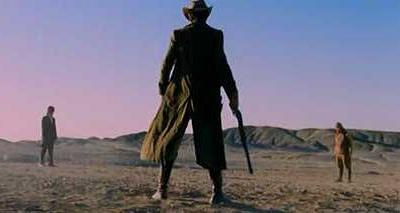
\includegraphics[width=0.8\textwidth,height=120pt]{corral.jpg}
  %\caption{}\label{}
\end{figure}
\end{spacing}
\end{frame}
\begin{frame}[t]{The Shootout}
\begin{spacing}{1.1}
Let us discuss the last example in more detail: Let $P(n)$ be the statement
that there is at least one survivor whenever $2n+1$ people, fire pistols at
each other in the same instant. Each person fires at his nearest neighbor,
and all people stand at mutually distinct distances to each other.\\[5pt]
For $n=1$, there are three people, A, B and C. Suppose that the distance between A and B is the smallest distance of any two of them. Then A fires at B and vice-versa. C fires at either A or B and will not be fired at, so C survives.\\[5pt]
Suppose $P(n)$. Let $2n+3$ people participate in the shootout. Suppose that
A and B are the closest pair of people. The A and B fire at each other.
\begin{itemize}
  \item If at least one other person fires at A or B, then there remain at most
      $2n$ shots fired among the remaining $2n + 1$ people, so there is at least
      one survivor.
  \item If no-one else fires at A or B, then there are $2n+1$ shots fired among the $2n+1$ people and by $P(n)$, there is at least one survivor.
\end{itemize}
\end{spacing}
\end{frame}
\begin{frame}[c,allowdisplaybreaks,allowframebreaks]{Pitfalls in Induction}
\begin{spacing}{1.05}
While mathematical induction is an extremely powerful technique, it must
be executed most carefully. In proceeding through an induction proof it
can happen quite easily that implicit assumptions are made that are not
justified, thereby invalidating the result.\\[5pt]
\alert{1.3.5. Example.} Let us use mathematical induction to argue that every set of $n\geq2$ lines in the plane, no two of which are parallel, meet in a common point.\\[4pt]
The statement is true for $n = 2$, since two lines are not parallel if and only
if they meet at some point. Since these are the only lines under
considerations, this is the common meeting point of the lines.\\[4pt]
We next assume that the statement is true for n lines, i.e., any $n$
non-parallel lines meet in a common point. Let us now consider $n + 1$
lines, which we number 1 through $n +1$. Take the set of lines 1 through $n$;
by the induction hypothesis, they meet in a common point. The same is
true of the lines $2,\,...\,,n+1$. We will now show that these points must be
identical.
\newpage
Assume that the points are distinct. Then all lines $2,\,...\,,n$ must be the
same line, because any two points determine a line completely. Since we
can choose our original lines in such a way that we consider distinct lines,
we arrive at a contradiction. Therefore, the points must be identical, so all
$n + 1$ lines meet in a common point. This completes the induction proof.\\[6pt]
Where is the mistake in the above ``proof'' of our (obviously false) supposition?
\end{spacing}
\end{frame}
\begin{frame}[t]{Strong (Complete) Induction}
\begin{spacing}{0.95}
The method of induction can be strengthened. We can replace
\begin{itemize}
  \item[(I)] $A(n_0)$ is true.
  \item[(II)] $A(n+1)$ is true whenever $A(n)$ is true for $n\geq n_0$.
\end{itemize}
with
\begin{itemize}
  \item[(I)] $A(n_0)$ is true.
  \item[(II')] $A(n+1)$ is true whenever all the statements\\
      $A(n_0),A(n_0+1),\,...\,,A(n)$ are true.
\end{itemize}
\alert{1.3.6. Example.} We will show the following statement: \emph{Every natural number $n\geq2$ is a prime number or the product of primes.}\\[3pt]
Clearly the statement is true for $n=2$, which is prime. Next assume that $2,3,\,...\,,n$ are all prime or the product of prime numbers. Then $n+1$ is either prime or not prime. If it is prime, we are finished. If it is not prime, it is the product of two numbers $a,b<n+1$. However, $a$ and $b$ are themselves products of prime numbers by our assumption, and hence so is $n+1=a\cdot b$. Therefore, by the strong induction principle the initial statement is true.
\end{spacing}
\end{frame}
\begin{frame}[t,allowdisplaybreaks,allowframebreaks]{Induction vs. Strong Induction}
\begin{spacing}{1.05}
While induction is the principle that
\begin{equation}\label{1.3.2}
\Big(A(n_0)\wedge\mathop{\forall}_{\begin{subarray}{c}
                                     n\in\N\\
                                     n\geq n_0
                                   \end{subarray}}(A(n)\Rightarrow A(n+1))\Big)\Rightarrow\mathop{\forall}_{\begin{subarray}{c}
                                     n\in\N\\
                                     n\geq n_0
                                   \end{subarray}}A(n)
\end{equation}
strong induction states
\begin{equation}\label{1.3.3}
\Big(A(n_0)\wedge\mathop{\forall}_{\begin{subarray}{c}
                                     n\in\N\\
                                     n\geq n_0
                                   \end{subarray}}\big((A(n_0)\wedge\cdots\wedge A(n))\Rightarrow A(n+1)\big)\Big)\Rightarrow\mathop{\forall}_{\begin{subarray}{c}
                                     n\in\N\\
                                     n\geq n_0
                                   \end{subarray}}A(n).
\end{equation}
It is clear that \eqref{1.3.3} implies \eqref{1.3.2}, since of course
\[\big((A(n_0)\wedge\cdots\wedge A(n))\Rightarrow A(n+1)\big)\Rightarrow\big(A(n)\Rightarrow A(n+1)\big)\]
Thus the ``usual'' induction is a special case of strong induction. However,
the converse is also true, as we shall see.
\end{spacing}
\newpage
\begin{spacing}{0.9}
We now show that \eqref{1.3.2} implies \eqref{1.3.3}, i.e., strong induction follows from induction.\\[4pt]
We fix $n_0\in\N$ and define $B(n):A(n_0)\wedge\cdots\wedge A(n)$ for $n\geq n_0$. Then $A(n_0)=B(n_0)$ and we can write strong induction as
\[\Big(B(n_0)\wedge\mathop{\forall}_{\begin{subarray}{c}
                                     n\in\N\\
                                     n\geq n_0
                                   \end{subarray}}\big(B(n)\Rightarrow A(n+1)\big)\Big)\Rightarrow\mathop{\forall}_{\begin{subarray}{c}
                                     n\in\N\\
                                     n\geq n_0
                                   \end{subarray}}A(n).\]
\vspace*{-4pt}
We can write
\[\big(B(n)\Rightarrow A(n+1)\big)\equiv\big(B(n)\Rightarrow(A(n+1)\wedge B(n))\big)\equiv\big(B(n)\Rightarrow B(n+1)\big)\]
so strong induction becomes
\begin{equation}\label{1.3.4}
  \Big(B(n_0)\wedge\mathop{\forall}_{\begin{subarray}{c}
                                     n\in\N\\
                                     n\geq n_0
                                   \end{subarray}}\big(B(n)\Rightarrow B(n+1)\big)\Big)\Rightarrow\mathop{\forall}_{\begin{subarray}{c}
                                     n\in\N\\
                                     n\geq n_0
                                   \end{subarray}}A(n).
\end{equation}
Since $\displaystyle\mathop{\forall}_{\begin{subarray}{c}
                                     n\in\N\\
                                     n\geq n_0
                                   \end{subarray}}A(n)\equiv\mathop{\forall}_{\begin{subarray}{c}
                                     n\in\N\\
                                     n\geq n_0
                                   \end{subarray}}B(n)$
we see that \eqref{1.3.4} is just induction in $B$.
\end{spacing}
\end{frame}
\begin{frame}[t]{Recursive Definitions and the Factorial}
\begin{spacing}{0.95}
The induction axiom also allows us to make \emph{recursive definitions}. For
example, we wish to define a function (to be called the \emph{factorial})
\[(\,\cdot\,)!\!:\N\to\N\]
having the properties that
\begin{equation}\label{1.3.5}
  0!:=1,\qquad\quad n!:=n\cdot(n-1)!,\qquad\quad
  n\in\N\setminus\{0\}.
\end{equation}
This is an example of a \emph{recursive definition} and we may ask whether such a
definition ``makes sense'', i.e., whether such a function \textcolor[rgb]{1.00,0.00,0.00}{exists} and is \textcolor[rgb]{1.00,0.00,0.00}{unique}.\\[4pt]
That such recursive definitions define unique functions on $\N$ can be shown
using the induction axiom. We refer again to Halmos's book for the
details. In the present case, the function is simply
\begin{equation}\label{1.3.6}
  n!:=\prod_{k=1}^{n}k,\qquad\qquad\quad
  n\in\N\setminus\{0\},
\end{equation}
\end{spacing}
\end{frame}
\begin{frame}[t]{Recursive Definitions}
\begin{spacing}{1.05}
The definition \eqref{1.3.5} is called an \emph{inductive} or \emph{recursive formula} for $n!$, while \eqref{1.3.6} is called a \emph{closed formula} for $n!$. Recursive definitions often
occur naturally in the formulation of a problem, and finding a closed
formula can be extremely difficult. In some situations, a closed formula is highly desirable, while at other times, important properties are best
expressed through recursive expressions.\\[4pt]
For example, there exists a continuous extension of the factorial, given by
the \emph{Euler gamma function}, defined for $t>0$,
\[\Gamma(t):=\int_{0}^{\infty}z^{t-1}e^{-z}\,dz,
\qquad\qquad t>0.\]
It is possible to show that $\Gamma(1)=1$ and that
\[\Gamma(t+1)=t\Gamma(t)=t\Gamma\big((t-1)+1\big)\qquad\quad
\text{for}\,t>0.\]
\end{spacing}
\end{frame}
\begin{frame}[t]{Justification of Recursive Definitions}
\begin{spacing}{1.05}
Comparing with \eqref{1.3.5}, we see that
\[\Gamma(n+1)=n!\qquad\qquad\qquad
\text{for}~n\in\N.\]
Since the gamma function is defined for all strictly positive real numbers,
we have a ``continuous extension'' of the factorial.\\[5pt]
A slight modification allows for recursive definitions ``starting'' at $n=n_0$ instead of $n=0$. Furthermore, we can define functions not just based on
their preceding value, but on several such values.\\[5pt]
\alert{1.3.7. Example.} The \emph{Fibonacci sequence }is defined through
\[f_0:=0,\qquad f_1:=1,\qquad f_n:=f_{n-1}+f_{n-2},\qquad n\in\N\setminus\{0,1\}.\]
This type of recursive definition also follows from the induction axiom,
much as strong induction does.
\end{spacing}
\end{frame}
\begin{frame}[c]{Recursive Definitions of Sets}
\begin{spacing}{1.1}
In the same manner, we can define subsets of $\N$ recursively. For example, consider the set $S\subset\N$ such that
\begin{equation}\label{1.3.7}
  3\in S\qquad\qquad\text{and}\qquad\qquad
  x,y\in S\Rightarrow x+y\in S.
\end{equation}
(The validity of such a recursive definition (that a set $S$ with the
properties \eqref{1.3.7} exists and is unique) is based on the induction axiom.) We know that $3\in S$, so $3+3=6\in S,\,3+6=9\in S,\,6+6=12\in S$ and so on. Our goal is to prove that
\[S=\{n\in\N\!:\exists k\in\N\setminus\{0\}\!:\,n=3k\}.\]
However, this requires a little preparation.
\end{spacing}
\end{frame}
\begin{frame}[t,label=1.3.8]{Alphabets and Strings}
\begin{spacing}{1.05}
We introduce an example from the theory of formal languages:\\[6pt]
\alert{1.3.8. Definition.} An \emph{alphabet} $\Sigma$ is a finite, non-empty set of elements called \emph{symbols}. We define the set $\Sigma^*$ of \emph{strings} (or \emph{words}) over $\Sigma$ as follows:
\begin{itemize}
  \item[(i)] $\lambda\in\Sigma^*$, where $\lambda$ is the \emph{empty string (null string)} containing no symbols.
  \item[(ii)] If $w\in\Sigma^*$ and $x\in\Sigma$, then $wx\in\Sigma^*$.
\end{itemize}
\vspace*{6pt}
\alert{1.3.9. Example.} Let $\Sigma=\{0,1\}$. The elements of $\Sigma$ are called \emph{bits} and the words over $\Sigma$ are called \emph{bit strings}. $\lambda$ is a word, so also $\lambda0=0$ is a word, as is $\lambda1=1$. Since $\{0,1\}\subset\Sigma^*$, the two-symbol words $01,10,11,00\in\Sigma^*$ and, continuing, $000,001,010,011,100,101,110,111\in\Sigma^*$. In this way, we inductively find all words over $\Sigma$.\\[5pt]
We may interpret strings as tuples or finite sequences, but that is not
necessary.
\end{spacing}
\end{frame}
\begin{frame}[t]{Bit Strings in Logic}
\begin{spacing}{1}
\vspace*{-5pt}
Bit strings can be used in logic programming by replacing the values $T$
and $F$ by 1 and 0, respectively. Logical operations then become
analogously defined bit operations. In particular, $\neg$ becomes NOT, $\wedge$ becomes AND, $\vee$ becomes OR, where (for example)
\begin{center}
  \begin{tabular}{c|c}
    $b$ & $\text{NOT}\,b$ \\ \hline
    1 & 0 \\
    0 & 1 \\
  \end{tabular}
  \qquad
  \begin{tabular}{c|c|c}
    $a$ & $b$ & $a\,\text{AND}\,b$ \\ \hline
    1 & 1 & 1 \\
    1 & 0 & 0 \\
    0 & 1 & 0 \\
    0 & 0 & 0 \\
  \end{tabular}
  \qquad
  \begin{tabular}{c|c|c}
    $a$ & $b$ & $a\,\text{OR}\,b$ \\ \hline
    1 & 1 & 1 \\
    1 & 0 & 1 \\
    0 & 1 & 1 \\
    0 & 0 & 0 \\
  \end{tabular}
\end{center}
Given a bit string we then define corresponding \emph{bitwise operations}
recursively. For example,
\[\text{NOT}(\lambda):=\lambda,\qquad
\text{NOT}(wx):=\text{NOT}(w)\text{NOT}(x),\qquad
w\in\Sigma^*,~x\in\Sigma.\]
Thus
\[\text{NOT}(011)=\text{NOT}(01)\text{NOT}(1)=\text{NOT}(0)
\text{NOT}(1)\text{NOT}(1)=100.\]
\end{spacing}
\end{frame}
\begin{frame}[t,label=Concatenation]{Concatenation of Strings}
\begin{spacing}{1.05}
To denote a non-empty word $w\neq\lambda$, we often write $wx$, where $w\in\Sigma^*$ and $x\in\Sigma$.\\[5pt]
\alert{1.3.10. Definition.} We define \emph{concatenation of strings} as follows:
\begin{itemize}
  \item[(i)] If $w\in\Sigma^*$, then $w\cdot\lambda=w$, where $\lambda$ is the empty string.
  \item[(ii)] If $w_1,w_2\in\Sigma^*,x\in\Sigma$, then
      \[w_1\cdot(w_2x)=(w_1\cdot w_2)x.\]
\end{itemize}
\vspace*{4pt}
This recursive definition is a bit difficult to read at first, so we give an
example.\\[5pt]
\alert{1.3.11. Example.} Let $\Sigma=\{0,1\}$. The concatenation of $110,101\in\Sigma^*$ according to Definition \hyperlink{Concatenation}{1.3.10} is computed as follows:
\begin{equation*}
  \begin{split}
     \mathop{110}_{w_1}\cdot\,(\mathop{10}_{w_2}\mathop{1}_{x}) &=(110\cdot10)1=\big((110\cdot1)1\big)1 \\
       &=\big(\big((110)1\big)0\big)1=110101.
  \end{split}
\end{equation*}
\end{spacing}
\end{frame}
\begin{frame}[c,label=1.3.12]{Length of Strings}
\begin{spacing}{1.1}
Definition \hyperlink{Concatenation}{1.3.10} thus reduces the concatenation of strings to the concatenation of a string with a symbol, which we know how to do from Definition \hyperlink{1.3.8}{1.3.8}. In other words, we concentrate words by appending one symbol at a time. We make one more definition:\\[5pt]
\alert{1.3.12. Definition.} We define the \emph{length $I(w)$ of a string $w\in\Sigma^*$} as follows:
\begin{itemize}
  \item[1.] $I(\lambda)=0$,
  \item[2.] $I(wx)=I(w)+1$, where $x\in\Sigma$.
\end{itemize}
\vspace*{6pt}
\alert{1.3.13. Remark.} Since the set $\Sigma^*$ is not a subset of the natural numbers, it
may be asked whether a set with the properties of Definition \hyperlink{1.3.8}{1.3.8} exists uniquely. That this is the case is an axiom of set theory, i.e., it is assumed
that such recursive definitions ``work''.
\end{spacing}
\end{frame}
\begin{frame}[t,allowdisplaybreaks,allowframebreaks]{Structural Induction}
\begin{spacing}{1.1}
\vspace*{10pt}
Structural induction is a useful variant of induction that allows us to prove
properties for recursively defined objects, such as the strings we have just
introduced.\\[5pt]
Structural induction establishes a statement on a recursively defined set in
two steps. We call those elements specifically included in the set (e.g., the
empty string in $\Sigma^*$) the basis elements of the set.
\begin{itemize}
  \item[1.] Establish the statement for the basis elements.
  \item[2.] Show that if the statement is true for each of the elements used to
      construct new elements in the recursive step of the definition, the
      statement holds for these new elements.
\end{itemize}
\end{spacing}
\newpage
\begin{spacing}{1}
As a first example, consider a proposition $P(w)$, where $w\in\Sigma^*$ is a string. In order to prove that $P(w)$ is true for all $w\in\Sigma^*$, we need to show
\begin{itemize}
  \item[1.] $P(\lambda)$, where $\lambda$ is the empty string.
  \item[2.] $\mathop{\forall}\limits_{w\in\Sigma^*}\mathop{\forall}\limits_{x\in\Sigma}P(w)\Rightarrow P(wx).$
\end{itemize}
\alert{1.3.14. Example.} We prove that $I(xy)=I(x)+I(y)$ for $x,y\in\Sigma^*$, where $I(w)$ is the length of a string $w\in\Sigma^*$, cf. Definition \hyperlink{1.3.12}{1.3.12}.\\[4pt]
We need to formulate the statement in such a way that we can employ
induction. Let us write it as
\[P(y)\!:\mathop{\forall}_{x\in\Sigma^*}I(xy)
=I(x)+I(y).\]
We first establish $P(\lambda)$. This is the statement
\[P(\lambda)\!:\mathop{\forall}_{x\in\Sigma^*}I(x\lambda)
=I(x)+I(\lambda).\]
Since $x\lambda=x$ and $I(\lambda)=0,\,P(\lambda)$ is true.
\end{spacing}
\newpage
\begin{spacing}{1.1}
Next, assume that $P(y)$ is true. We must now show that $P(ya)$ is true for all $a\in\Sigma$, i.e.,
\[P(y)\Rightarrow\mathop{\forall}_{a\in\Sigma}P(ya)\]
or
\[\Big(\mathop{\forall}_{x\in\Sigma^*}I(xy)=I(x)+I(y)\Big)\Rightarrow
\Big(\mathop{\forall}_{a\in\Sigma}\mathop{\forall}_{x\in\Sigma^*}I(xya)=I(x)+I(ya)\Big)\]
Since $I(xya)=I(xy)+1$ and $I(ya)=I(y)+1$ by Definition \hyperlink{1.3.12}{1.3.12}, the implication follows and the proof is complete.\\[5pt]
The justification for structural induction lies in ordinary induction, applied
to the statement
\begin{align*}
  P(n)\!: &~\text{The claim is true for all elements of the set generated with}~n  \\
   &~\text{or fewer applications of the recursive rules for the set.}
\end{align*}
Structural induction first establishes $P(0)$ and then $P(n)\Rightarrow P(n+1)$.
\end{spacing}
\end{frame}
\begin{frame}[c,allowdisplaybreaks,allowframebreaks]{Explicit Representation of Recursively Defined Sets}
\begin{spacing}{1.1}
Let us return to our original example: Define $S\subset\N$ to be the set such that
\begin{itemize}
  \item[(i)] $3\in S$,
  \item[(ii)] $x,y\in S\Rightarrow x+y\in S$.
\end{itemize}
We want to show that $S=T$.\\[5pt]
First, we show $S\subset T$ by structural induction: $3=3\cdot1\in T$, so the base case is established. Now for $x,y\in S$ suppose that $x,y\in T$ so that $x=3k$ and $y=3k'$ for $k,k'\in\N\setminus\{0\}$. Then
\[x+y=3k+3k'=3(k+k')\]
so $x+y\in T$. This shows that $S\subset T$.
\newpage
Next, we show $T\subset S$ by (ordinary) induction. We claim that
\[\mathop{\forall}_{k\in\N\setminus\{0\}}3k\in S.\]
For $k=1,\,3k=3\cdot1=3\in S$, so the base case is established. Now suppose that $3k\in S$. Since $3\in S$ by definition, we can apply the recursive rule for $S$ to deduce that
\[3(k+1)=3k+3\in S.\]
This shows that $3(k+1)\in S$ if $3k\in S$. By the structural induction principle, $3k\in S$ for all $k\in\N\setminus\{0\}$. This established $T\subset S$.\\[6pt]
We finally conclude that $S=T$.
\end{spacing}
\end{frame}
\subsection{Equivalence Relations, Integers, Rationals}
\begin{frame}[c] \begin{spacing}{2}
\tableofcontents[sectionstyle=hide,subsectionstyle=show/shaded/hide]
\end{spacing}
\end{frame}
\begin{frame}[t]{Structure for Numbers}
\begin{spacing}{1.1}
In mathematics, it is frequently useful to classify diverse objects into
abstract frameworks. Understanding the abstract framework then gives an
understanding of these various concrete objects, which superficially may
appear quite unrelated.\\[6pt]
An example of this from linear algebra is the concept of a vector space: By
understanding concepts in general vector space (such as linear
independence, bases, norms, inner products), the corresponding results can
be applied to various objects, such as
\begin{itemize}
  \item Euclidean space $\R^n$
  \item The set of continuous functions on an interval
  \item The set of solutions to a system of linear algebraic equations
  \item The set of solutions to a single homogeneous, linear differential equation
\end{itemize}
\end{spacing}
\end{frame}
\begin{frame}[t]{Groups}
\begin{spacing}{1.1}
We aim to find an analogous structure for \emph{numbers}, in the hopes that later
other objects can be subsumed in this structure. In particular, we would
like the set of numbers, together with the operation of addition, to form a
group.\\[5pt]
\alert{1.4.1. Definition.} A \emph{group} is a pair $(G,\circ)$ consisting of a set $G$ and a \emph{group operation} $\circ\!:\,G\times G\to G$ such that
\begin{itemize}
  \item[(i)] $a\circ(b\circ c)=(a\circ b)\circ c$ for all $a,b,c\in G$\,\alert{(associativity)},
  \item[(ii)] there exists an element $e\in G$ such that $a\circ e=e\circ a=a$ for all $a\in G$ \alert{(existence of a unit element)},
  \item[(iii)] for every $a\in G$ there exists an element $a^{-1}\in G$ such that $a\circ a^{-1}=a^{-1}\circ a=e$ \alert{(existence of an inverse)}.
\end{itemize}
A group is called \emph{abelian} if in addition to the above properties
\begin{itemize}
  \item[(iv)] $a\circ b=b\circ a$ for all $a,b\in G$ \alert{(commutativity)}.
\end{itemize}
\end{spacing}
\end{frame}
\begin{frame}[c]{The Natural Numbers are not a Group}
\begin{spacing}{1.1}
It is easy to check that $(\N,+)$ satisfies the properties
\begin{itemize}
  \item[(i)] $a+(b+c)=(a+b)+c$ for all $a,b,c\in\N$,
  \item[(ii)] $0\in\N$ satisfies $a+0=0+a=a$ for all $a\in\N$,
  \item[(iv)] $a+b=b+a$ for all $a,b\in\N$.
\end{itemize}
However, it is not true that
\begin{itemize}
  \item[(iii)] for every $a\in\N$ there exists an element $a^{-1}\in\N$ such that $a+a^{-1}=a^{-1}+a=0$.
\end{itemize}
\vspace*{6pt}
Therefore, we need to expand the set of natural numbers to a larger set
(which we will call the \emph{integers}). In order to construct this set, we need to
first digress to some material from Chapter 8 of Rosen's textbook.
\end{spacing}
\end{frame}
\begin{frame}[t,allowdisplaybreaks,allowframebreaks]{Relations}
\begin{spacing}{1.1}
\vspace*{9pt}
Given two sets, the elements of these sets may be paired together in a
certain way. A more precise formulation is given by the concept of a
\emph{relation}, which we now introduce.\\[6pt]
\alert{1.4.2. Examples.}
\begin{itemize}
  \item For $n\in\N,\,n\mapsto n^2$ associates to every number $n$ its square $n^2$.
  \item $n^3\mapsto n$ associates to some numbers $n^3=p\in\N$ the number $n$.
\end{itemize}
We implement this by defining a relation $R$ to be a set of ordered pairs. In
the above examples, we might define
\begin{align*}
  R &=\{(a,b)\in\N^2\!:\,b=a^2\}, \\
  R &=\{(a,b)\in\N^2\!:\,a=b^3\},
\end{align*}
\end{spacing}
\newpage
\begin{spacing}{0.95}
We define a \emph{relation R between two sets M and N} to be the set
\setcounter{equation}{0}
\begin{equation}\label{1.4.1}
  R=\{(m,n)\in M\times N\!:\,P(m,n)\}
\end{equation}
where $P$ is a statement frame (predicate). If $M=N$, we say that $R$ is a \emph{relation on M}.\\[5pt]
Thereby the \emph{active} concept of a relation (we associate one number to
another; we do something) is defined by the \emph{static} concept of a set (no
action takes place; $R$ is just an object). This is a fairly modern idea in
mathematics.\\[5pt]
Instead of writing $(a,b)\in R$, we often write $a\sim_R b$ (or $a\sim b$ if the relation $R$ is clear from the context).\\[4pt]
We define the \emph{domain} of a relation $R$ by
\[\text{dom}\,R=\{a\!:\exists b\!:(a,b)\in R\}\]
and the \emph{range} by
\[\text{ran}\,R=\{b\!:\exists a\!:(a,b)\in R\}.\]
\end{spacing}
\end{frame}
\begin{frame}[t]{Equivalence Relations}
\begin{spacing}{1.05}
\alert{1.4.3. Definition.} We say that a relation $R$ on a set $M$ is
\begin{itemize}
  \item[(i)] \emph{reflexive} if $(a,a)\in R$ for all $a\in M$;
  \item[(ii)] \emph{symmetric} if $(a,b)\in R$ implies $(b,a)\in R$ for all $a,b\in M$;
  \item[(iii)] \emph{anti-symmetric} if $(a,b)\in R$ and $(b,a)\in R$ implies $a=b$ for all $a,b\in M$;
  \item[(iv)] \emph{transitive} if $(a,b)\in R$ and $(b,c)\in R$ implies $(a,c)\in R$ for all $a,b,c\in M$.
\end{itemize}
A reflexive, symmetric and transitive relation on $M$ is called an \emph{equivalence relation on M}. In more intuitive notation\\[5pt]
\begin{itemize}
  \item reflexivity means $a\sim a$ for all $a\in M$,
  \item symmetry means $a\sim b\Rightarrow b\sim a$ for all $a,b\in M$,
  \item anti-symmetry means $(a\sim b\wedge b\sim a)\Rightarrow a=b$ for all $a,b\in M$,
  \item transitivity means $a\sim b\wedge b\sim c\Rightarrow a\sim c$ for all $a,b,c\in M$.
\end{itemize}
\end{spacing}
\end{frame}
\begin{frame}[t]{Relations}
\begin{spacing}{1.1}
\alert{1.4.4. Examples.}
\begin{itemize}
  \item The relation $R=\{(a,b)\in\N^2\!:a>b\}$ includes the pairs $(1,0),(2,1),(2,0)$ but not the pair $(0,1)$. We write $(a,b)\in R\Leftrightarrow a\sim b\Leftrightarrow a>b$ and notice that $\sim$ is transitive (since $a>b$ and $b>c$ implies $a>c$), but not symmetric $(a>b\nRightarrow b>a)$ or reflexive $(a\ngtr a)$.
  \item For $n\in\N$ we define the \emph{integer sum} $I(n)$ as the sum of all integers that compose the number, e.g., $I(125)=1+2+5=8,\,I(78)=7+8=15$.\\[5pt]
      Then the relation $R=\{(a,b)\in\N^2\!:\,I(a)=I(b)\}$ includes the pairs $(22,4),(14,5),(3,30)$ but not the pair $(4,1)$. We note that $R$ is reflexive $(I(a)=I(a))$, symmetric (if $I(a)=I(b)$, then also $I(b)=I(a)$) and transitive (if $I(a)=I(b)$ and $I(b)=I(c)$, then $I(a)=I(c)$), so $R$ is an equivalence relation. We may then call all numbers with equal integer sums \emph{equivalent} in this sense.
\end{itemize}
\end{spacing}
\end{frame}
\begin{frame}[t,allowdisplaybreaks,allowframebreaks]{Equivalence Classes}
\begin{spacing}{1.2}
A partition of a set $A$ is a family $\mathcal{F}$ of disjoint subsets of $A$ such that their
union is $A$. An element of a partition is called a \emph{fiber} or an \emph{equivalence
class}. An element of such an equivalence class is called a \emph{representative} of
the class.\\[6pt]
\alert{1.4.5. Example.} Denote by $2\N=\{0,2,4,6,\,...\}\subset\N$ the set of all even natural numbers and by $2\N+1=\{1,3,5,7,\,...\}\subset\N$ the set of all odd natural numbers. Since\\[3pt]
\[2\N\cap(2\N+1)=\emptyset\qquad\qquad
\text{and}\qquad\qquad
2\N\cup(2\N+1)=\N\]
it follows that $\mathcal{F}=\{2\N,2\N+1\}$ is a partition of $\N$ and $2\N$ and $2\N+1$ are the two equivalence classes of this partition. The number 4 is a representative of $2\N$, as are 0, 128 and 456, and the numbers 1, 7, 457 are representatives of $2\N+1$.
\newpage
We often denote equivalence classes by one of their representatives
enclosed in square brackets, so we might write
\[2\N=[0]\qquad\qquad
\text{and}\qquad\qquad
2\N+1=[1].\]
\alert{1.4.6. Theorem.} Every partition $\mathcal{F}$ of $M$ induces an equivalence relation $\sim$ on a set $M$ by
\begin{equation}\label{1.4.2}
  a\sim b\qquad\quad:\Leftrightarrow\qquad
  a,b\in M~\text{are in the same equivalence class.}
\end{equation}
 \\[7pt]
\alert{Proof.}\\
It is easily seen that the relation $\sim$ defined by \eqref{1.4.2} is reflexive, symmetric and transitive.
\multido{}{14}{\qquad}\quad$\square$
\end{spacing}
\end{frame}
\begin{frame}[t,allowdisplaybreaks,allowframebreaks]{{\large Fundamental Theorem on Partitions and Equivalence Relations}}
\begin{spacing}{1.1}
\vspace*{9pt}
\alert{1.4.7. Theorem.} Every equivalence relation $\sim$ on a set $M$ induces a partition $\mathcal{F}=\{[a]\!:\,a\in M\}$ of $M$ by
\begin{equation}\label{1.4.3}
a\in[b]\qquad\qquad\qquad:\Rightarrow\qquad
\qquad\qquad a\sim b.
\end{equation}
We write $\mathcal{F}=M/\sim.$\\[7pt]
\alert{Proof.}\\
We need to prove that $\mathcal{F}$ is a partition, i.e., that the union of all classes in $\mathcal{F}$ is $M$ and that classes are disjoint.\\[6pt]
Since $\sim$ is \textbf{reflexive}, it follows that $a\in[a]$ for every $a\in M$, so every $a$ is in some class. Thus, the union of all classes is $M$.
\newpage
\alert{Proof (continued).}\\
We next show that the classes are disjoint. Let $[a],[b]$ be two classes. Assume that there is an element $c\in M$ such that $c\in[a]$ and $c\in[b]$, so $c\sim b$ and $c\sim a$.\\[6pt]
Let $x\in[a]$ be an arbitrary element. Then by \textbf{symmetry} and \textbf{transitivity}
\begin{equation*}
  \begin{split}
     x\in[a]\qquad &\Rightarrow\qquad x\sim a\qquad\Rightarrow\qquad a\sim x\qquad\Rightarrow\qquad c\sim x \\
       &\Rightarrow\qquad x\sim c\qquad\Rightarrow\qquad x\sim b\qquad\Rightarrow\qquad x\in[b]
  \end{split}
\end{equation*}
so $[a]\subset [b]$.\\[4pt]
Changing the roles of $a$ and $b$, we have $[b]\subset[a]$, hence $[a]=[b]$. Thus, if two classes have a single element in common, they are the same class. Hence, the classes are disjoint.
\begin{flushright}
  $\square$
\end{flushright}
\end{spacing}
\end{frame}
\begin{frame}[t,allowdisplaybreaks,allowframebreaks]{The Integers}
\begin{spacing}{1}
We will now introduce the negative numbers. One big deficiency in the
natural numbers is that there is no \emph{inverse element} for addition, i.e., for every $n\in\N$ we would like to have an element $-n$ such that
\[n+(-n)=0\]
Such an element does not exist in $\N$. We therefore consider the set of ordered pairs
\[\N^2=\{(n,m)\!:\,m,n\in\N\}.\]
We can consider $\N$ as a natural subset of $\N^2$ by replacing $n\in\N$ with $(n,0)\in\N^2$. Furthermore, we define the following equivalence relation on $\N^2$:
\begin{equation}\label{1.4.4}
  (n,m)\sim(p,q)\qquad\quad:\Leftrightarrow\qquad\quad
  n+q=m+p.
\end{equation}
Therefore, the pair $(5,0)$ (which corresponds to $5\in\N$) is equivalent to $(6,1)$, because $5+1=0+6$.
\end{spacing}
\newpage
\begin{spacing}{1.15}
\vspace*{8pt}
We have the following facts:
\begin{itemize}
  \item \eqref{1.4.4} defines an equivalence relation, which induces a partition $\Z=\N^2/\sim\,\text{on}\,\N^2$.
  \item Every pair of the form $(n,0)\in\N^2,\,n\in\N$, is in a different equivalence class of this partition. We denote these equivalence classes by $[+n]\ni(n,0)$.
  \item Every pair of the form $(0,n)\in\N^2,\,n\in\N,\,n\geq1$, is in yet another equivalence class, denoted by $[-n]\ni(0,n)$.
  \item Any other pair is in a class $[+n]$ or a class $[-n]$ for some $n\in\N$.
  \item It follows that
  \[\Z=\{[+n]\!:\,n\in\N\}\cup\{[-n]\!:\,n\in\N\setminus\{0\}\}.\]
\end{itemize}
\newpage
We now want to define addition for elements of $\N^2$ by
\begin{equation}\label{1.4.5}
  (n,m)+(p,q)=(n+p,m+q).
\end{equation}
If $(n,m)\sim(\widetilde{n},\widetilde{m})$ and $(p,q)\sim(\widetilde{p},\widetilde{q})$, then
\begin{equation}\label{1.4.6}
(n,m)+(p,q)\sim(\widetilde{n},\widetilde{m})+(\widetilde{p},\widetilde{q}).
\end{equation}
This means that we can define the sum of two equivalence classes by \eqref{1.4.5}: let $[\pm n],[\pm m]\in\Z$. Then we define $[\pm n]+[\pm m]$ as the class whose representatives are obtained by adding any representative of $[\pm n]$ to any representative of $[\pm m]$ according to \eqref{1.4.5}. The fact that the result does not depend on which representative we choose is expressed by \eqref{1.4.6}.\\[5pt]
We say that the so defined addition on $\Z$ is \emph{independent of the chosen representative} and therefore \emph{well-defined}.
\end{spacing}
\newpage
\begin{spacing}{1}
Note that
\[(n,m)+(0,0)=(n,m),\qquad (n,m)+(p,q)=(p,q)+(n,m)\]
and we also have the associative law of addition. Therefore, the addition on $\Z$ also has these properties and $[0]\in\Z$ is the neutral element of addition.\\[5pt]
Furthermore, let $(n,m)\in\N^2$. Then
\[(n,m)+(m,n)=(n+m,n+m)\sim(0,0).\]
In particular, $[n]+[-n]=[0]$. so we now have an inverse element for the addition defined on $\Z$.\\[5pt]
The set $\Z$ is known as the set of \emph{integers}. We write $n$ instead of $[n]$ and $-n$ instead of $[-n]$. Furthermore, we abbreviate $n+(-m)$ by $n-m$ and call the ``operation'' - \emph{subtraction}. The letter $\Z$ is used for historical reasons: it stands for the German word for numbers, \emph{Zahlen}.
\newpage
Let us review our strategy up to this point:
\begin{itemize}
  \item The set of natural numbers was too small, because it didn't include
      an inverse element of addition.
  \item We introduce pairs of natural numbers and identify the natural numbers with certain pairs $(n\Leftrightarrow(n,0))$.
  \item We introduce a suitable equivalence relation on $\N^2$ and take $\Z=\N^2/\sim$ to be the induced partition.
  \item We characterize the partition $\Z=\{[n]\}\cup\{[-n]\}$.
  \item We define addition on $\N^2$ so that it is compatible with the previously defined addition on $\N$, i.e., we have $n\leftrightarrow(n,0),\,m\leftrightarrow(m,0)$ and $(n,0)+(m,0)$\\ $=(n+m,0)\leftrightarrow n+m$.
  \item We show that the addition on $\N^2$ is compatible with the equivalence classes and can hence be used to define the sum of two classes in $\Z$.
  \item We see that for the addition in $\Z$ we now have an inverse element for every element of $\Z$.
\end{itemize}
\end{spacing}
\end{frame}
\begin{frame}[t]{Multiplication}
\begin{spacing}{0.95}
The initial goal was to expand the natural numbers such as the new set of
numbers, together with the operation of addition, forms a group.\\[5pt]
However, we also need to discuss the effect of our extension on the
operation of multiplication. Based on the intuitive idea that
\[(m-n)\cdot(p-q)=m\cdot p+n\cdot q-m\cdot q-n\cdot p\]
we define multiplication on $\N^2$ by
\[(m,n)\cdot(p,q):=(m\cdot p+n\cdot q,\,m\cdot q+n\cdot p)\]
It will be shown in the assignments that this multiplication
\begin{itemize}
  \item allows the multiplication of the equivalence classes $[n]$ and $[-n]$, so that it is well-defined on $\Z=\N^2/\sim$,
  \item coincides with the known multiplication on $\N\subset\Z$,
  \item is associative and commutative and has the identity element $(1,0)$,
\end{itemize}
i.e., retains the properties of multiplication on $\N$ (see Slide \hyperlink{82}{82}).
\end{spacing}
\end{frame}
\begin{frame}[t,shrink,label=1.4.8]{Rings}
\begin{spacing}{0.9}
\alert{1.4.8. Definition.} A \emph{ring} is a triple $(R,+,\cdot)$ consisting of a set $G$ and two \emph{binary operations} $+,\cdot:\,R\times R\to R$ such that
\begin{itemize}
  \item[(i)] $(R,+)$ is an abelian group
  \item[(ii)] there exists an element $1\in R$ such that
      \[a\cdot1=1\cdot a=a\qquad\qquad\text{for all}~a\in R\]
      \alert{(existence of a multiplicative unit element)}
  \item[(iii)] for any $a,b,c\in R$,
      \[a\cdot(b\cdot c)=(a\cdot b)\cdot c\]
      \alert{(associativity)}
  \item[(iv)] for any $a,b,c\in R$,
      \[a\cdot(b+c)=(a\cdot b)+(a\cdot c),\qquad
      (b+c)\cdot a=(b\cdot a)+(c\cdot a)\]
      \alert{(distributivity)}
\end{itemize}
A ring is called \emph{commutative} if in addition to the above properties
\begin{itemize}
  \item[(iv)] $a\cdot b=b\cdot a$ for all $a,b\in R$ \alert{(commutativity)}
\end{itemize}
\end{spacing}
\end{frame}
\begin{frame}[c]{The Ring of the Integers}
\begin{spacing}{1.1}
\alert{1.4.9. Definition.} A ring $(R,+,\cdot)$ is said to be an \emph{integral domain} if
\[a\cdot b=0\qquad\qquad\quad
\Rightarrow\qquad\qquad\quad
a=0\quad\vee\quad b=0\]
for all $a,b\in R$.\\[5pt]
It can be shown that $\Z$ is a commutative integral domain with respect to addition and multiplication, but the proof is a little technical. See, for example,
\begin{center}
  \url{https://proofwiki.org/wiki/Ring_of_Integers_has_no_Zero_Divisors}
\end{center}
for details.
\end{spacing}
\end{frame}
\begin{frame}[t]{The Rationals}
\begin{spacing}{1}
We can of course now go further: the integers resulted from desiring an
inverse to the addition of natural numbers. However, the multiplication
still has no such inverse in the integers. We can now proceed as before:
We consider $\Z^2$, the set of pairs of integers. We define the equivalence relation
\begin{equation}\label{1.4.7}
(n,m)\sim(p,q)\qquad\qquad:\Leftrightarrow\qquad\qquad
n\cdot q=m\cdot p.
\end{equation}
for $(n,m),(p,q)\in\Z\times\Z\setminus\{0\}$. This is of course inspired by wanting
\[\frac{n}{m}=\frac{p}{q}.\]
We denote the set of rational numbers by $\Q:=(\Z\times\Z\setminus\{0\})/\sim$ and we consider $\Z$ as a subset of $\Z\times\Z\setminus\{0\}$ by associating $n\leftrightarrow(n,1)$.\\[5pt]
We will ordinarily identify a representative $(n,m)$ with its class $[(n,m)]$ and write
\[(n,m)=:\frac{n}{m}\in\Q.\]
\end{spacing}
\end{frame}
\begin{frame}[c]{Multiplication and Addition}
\begin{spacing}{1.1}
We define the product and sum of two pairs of integers by
\begin{align}\label{1.4.8}
  (n,m)\cdot(p,q) &:=(n\cdot p,m\cdot q) \\
  (m,n)+(p,q) &:=(q\cdot m+p\cdot n,nq).
\end{align}
As before, it can be shown that these operations can be used to define
addition and multiplication of classes in $\Q=(\Z\times\Z\setminus\{0\})/\sim$ and that they extend the previously defined operations on $\Z$ to $\Q$, preserving all the ring properties of Definition \hyperlink{1.4.8}{1.4.8}.\\[4pt]
The neutral element of multiplication is $[(1,1)]$ and every element $[(n,m)]\in\Q$ except $[(0,1)]$ has a multiplicative inverse
\[[(n,m)]^{-1}=[(m,n)].\]
\end{spacing}
\end{frame}
\begin{frame}[c]{Fields}
\begin{spacing}{1}
Of course, there is also a general algebraic structure to describe the
properties of the rational numbers:\\[5pt]
\alert{1.4.10. Definition.} Let $(F,+,\cdot)$ be a commutative ring with unit element of addition 0 and unit element of multiplication 1. Then $F$ is said to be a \emph{field} if
\begin{itemize}
  \item[(i)] $0\neq1$
  \item[(ii)] For every $a\in F\setminus\{0\}$ there exists an element $a^{-1}$ such that
      \[a\cdot a^{-1}=1.\]
\end{itemize}
Another way of writing this definition is to say that $(F,+,\cdot)$ is a field if $(F,+)$ and $(F\setminus\{0\},\cdot)$ are abelian groups, $0\neq1$ and the law of distributivity holds.\\[4pt]
Comparing with our previous construction, it is clear that $\Q$ is a field.
\end{spacing}
\end{frame}
\begin{frame}[c]{The Modulus of a Rational Number}
\begin{spacing}{1.1}
We introduce a final notation for later use: for any rational number $a\in\Q$, the symbol $|a|$ (called the \emph{modulus} or \emph{absolute value} of $a$) shall be defined as
\[|a|:=\left\{\begin{array}{lc}
                \!\!a & \text{if}~a\geq0, \\
                \!\!-a & \text{if}~a<0.
              \end{array}\right.\]
In the following section, we will proceed to investigate some of the number
sets we have just defined more closely, focusing particularly on the integers.
\end{spacing}
\end{frame}
\subsection{Functions, Sequence, Real Numbers}
\begin{frame}[c] \begin{spacing}{2}
\tableofcontents[sectionstyle=hide,subsectionstyle=show/shaded/hide]
\end{spacing}
\end{frame}
\begin{frame}[c]{Functions}
\begin{spacing}{1.1}
\setcounter{zhuo}{0}
\begin{DEFINITION}
Let $X$ and $Y$ be sets. A \emph{function from X to Y}, denoted $f:X\to Y$, is defined as a relation
\[f=\{(x,y)\in X\times Y:\,P(x,y)\}\]
for some predicate $P$ with the properties that
\setcounter{equation}{0}
\begin{equation}\label{1.5.1}
  \text{dom}\,f=X
\end{equation}
and
\begin{equation}\label{1.5.2}
  \mathop{\forall}_{(x_1,y_1)\in f}\mathop{\forall}_{(x_2,y_2)\in f}\quad(x_1=x_2~\Rightarrow~y_1=y_2).
\end{equation}
\end{DEFINITION}
The property \eqref{1.5.2} guarantees that for $(x,y)\in f$, $y$ is uniquely determined by $x$. We denote this $y$ by $y=f(x)$.
\end{spacing}
\end{frame}
\begin{frame}[t]{Domain, Range and Properties of Functions}
\begin{spacing}{1}
\begin{REMARK}
As for general relations, the domain and range are defined by
\begin{align*}
  \text{dom}\,f &=\{x:\exists y:(x,y)\in f\}. \\
  \text{ran}\,f &=\{y:\exists x:(x,y)\in f\}.
\end{align*}
\end{REMARK}
\begin{EXAMPLE}
\begin{itemize}
  \item $f=\{(x,y)\in\Z\times\Z\!:y=x^2\}$ is a function.
  \item $f=\{(x,y)\in\Z\times\Z\!:y^2=x^2\}$ is not a function since $(1,1)$ and $(1,-1)$ are both in $f$.
\end{itemize}
\end{EXAMPLE}
\begin{DEFINITION}
A function $f:X\to Y$ is said to be
\begin{itemize}
  \item \emph{injective} if $\mathop{\forall}\limits_{x_1,x_2\in X}\quad(f(x_1)=f(x_2)\Rightarrow x_1=x_2)$.
  \item \emph{surjective} if $\mathop{\forall}\limits_{y\in Y}\mathop{\exists}\limits_{x\in X}f(x)=y$.
  \item \emph{bijective} if $f$ is both injective and surjective.
\end{itemize}
\end{DEFINITION}
\end{spacing}
\end{frame}
\begin{frame}[t]{Inverse of a Functions}
\begin{spacing}{1.1}
Let
\[f=\{(x,y)\in X\times Y:\,P(x,y)\}\]
be a function. We define
\[f^{-1}:=\{(y,x)\in Y\times X:\,P(x,y)\}.\]
If $f$ is surjective, $f^{-1}$ satisfies property \eqref{1.5.1}. If $f$ is injective, $f^{-1}$ satisfies property \eqref{1.5.2}. We note:\\[5pt]
\stepcounter{zhuo}
\alert{1.5.5. Definition and Theorem.} If $f:X\to Y$ is a bijective function, the relation $f^{-1}:Y\to X$ (called the \emph{inverse function} to $f$) is a bijective function. Furthermore,
\[f^{-1}(f(x))=x\qquad\qquad\text{and}
\qquad\qquad f(f^{-1}(y))=y\]
\end{spacing}
\end{frame}
\begin{frame}[t]{Sequences}
\begin{spacing}{1.05}
One of the simplest type of functions are \emph{sequences of rational numbers},
functions $\N\to\Q$ or, more generally, $\Omega\to\Q$ where $\Omega\subset\N$. For example, we might have the sequence
\[\left\{\Big(n,\frac{1}{n}\Big):\,n\in\N\setminus\{0\}\right\}.\]
which has domain $\N\setminus\{0\}$.\\[4pt]
We denote a sequence with domain $\N$ by $(a_n)_{n\in\N}$, $(a_n)_{n=0}^\infty$ or simply $(a_n)$ and use analogous notations in case of smaller domains. We sometimes list a sequence by giving its values for $n=0,1,2,3,\,...\,.$\\[4pt]
\begin{EXAMPLE}
  The sequence $(a_n)\!:\,n\mapsto n^2$ can be written as
  \[(a_n)=(0,1,4,9,16,25,\,...),\]
  $(n^2)_{n\in\N}$ or as ``the sequence with values $a_n=n^2$.''
\end{EXAMPLE}
\end{spacing}
\end{frame}
\begin{frame}[t,allowdisplaybreaks,allowframebreaks]{Convergent and Cauchy Sequences}
\begin{spacing}{0.9}
It is assumed that sequences are familiar from calculus. We recall two
important concepts:\\[4pt]
\begin{DEFINITION}
  Let $(a_n)$ be a sequence of (for now, rational) numbers.
  \begin{itemize}
    \item[(i)] The sequence $(a_n)$ is said to \emph{converge with limit} $a\in\Q$ if
        \[\mathop{\forall}_{\varepsilon>0}\quad
        \mathop{\exists}_{N\in\N}\quad\mathop{\forall}_{n>N}
        \quad|a_n-a|<\varepsilon.\]
        We then write ``$\lim\limits_{n\to\infty}a_n=a$'' or ``$a_n\to a~\text{as}~n\to\infty$.''
    \item[(ii)] The sequence $(a_n)$ is said to be a \emph{Cauchy sequence} if
        \[\mathop{\forall}_{\varepsilon>0}\quad
        \mathop{\exists}_{N\in\N}\quad\mathop{\forall}_{m,n>N}
        \quad|a_n-a_m|<\varepsilon.\]
  \end{itemize}
\end{DEFINITION}
\begin{REMARK}
Since
\[|a_n-a_m|\leq|a_n-a|+|a_m-a|,\]
every convergent sequence is a Cauchy sequence,
\end{REMARK}
\end{spacing}
\newpage
\begin{spacing}{1.05}
However, not every Cauchy sequence of rational numbers converges. For
example, consider the sequence defined recursively as
\[a_0=1,\qquad\qquad a_{n+1}=\frac{4+3a_n}{3+2a_n},\qquad
n\in\N.\]
It is easy to see (by induction, if necessary) that $a_n\in\Q$ for all $n$. It can be shown that $(a_n)$ is a Cauchy sequence. Then the limit $a$, if it existed, would satisfy
\[a=\frac{4+3a}{3+2a}\qquad\qquad
\text{or}\qquad\qquad a^2=2.\]
But, as we will show later (Theorem \hyperlink{1.6.15}{1.6.15}),
there is no rational nuber satisfying $a^2=2$ so the limit can not exist in $\Q$.\\[5pt]
Our aim is to construct the \emph{completion} of the rational numbers by
``adding'' all the limits of Cauchy sequences to $\Q$.
\newpage
Given $\Q$, we may consider the set of all sequences in $\Q$ that converge to a limit. Denote this set by $\text{Conv}(\Q)$. Each sequence $(a_n)\in\text{Conv}(\Q)$ is associated uniquely to a number $a\in\Q$, namely its limit.\\[5pt]
We now say that two sequences are equivalent if they have the same limit,
i.e.,
\begin{equation}\label{1.5.3}
  (a_n)\sim(b_n)\qquad\qquad:\Leftrightarrow
  \qquad\qquad\lim_{n\to\infty}a_n=\lim_{n\to\infty}b_n.
\end{equation}
It is easy to check that this is an equivalence relation.\\[5pt]
We denote the equivalence class of all sequences with the same limit as a
sequence $(a_n)$ by $[(a_n)]$ and denote the corresponding partition by $\text{Conv}(\Q)/\sim$.\\[4pt]
Since each rational number is represented by a class (why?) we see that
the rational numbers may be identified with the set of all classes of
convergent sequences:
\[\Q\cong\text{Conv}(\Q)/\sim.\]
\end{spacing}
\end{frame}
\begin{frame}[t,allowdisplaybreaks,allowframebreaks]{Construction of the Real Numbers}
\begin{spacing}{1.1}
We can now consider a larger class of sequences, that of Cauchy sequences
of rational numbers, denoted by $\text{Cauchy}(\Q)$. Since every convergent sequence is a Cauchy sequence, $\text{Conv}(\Q)\subset\text{Cauchy}(\Q)$.\\[5pt]
Furthermore, we say that two Cauchy sequences are equivalent not if they
have the same limit (because they might not converge) but rather if their
difference converges to zero:
\begin{equation}\label{1.5.4}
  (a_n)\sim(b_n)\qquad\qquad:\Leftrightarrow
  \qquad\qquad\lim_{n\to\infty}(a_n-b_n)=0.
\end{equation}
Of course, \eqref{1.5.4} is equivalent to \eqref{1.5.3} for convergent sequences. We now have the larger set
\[\text{Cauchy}(\Q)/\sim\,\supset~\text{Conv}(\Q)/\sim
\,\simeq~\Q\]
\newpage
\vspace*{10pt}
The set $\text{Cauchy}(\Q)/\sim$ incorporates the rational numbers and by its construction every Cauchy sequence $(a_n)$ in $\text{Cauchy}(\Q)/\sim$ has a limit namely precisely the object represented by the class $[(a_n)]$. We write
\[\R:=\text{Cauchy}(\Q)/\sim\]
and call this set the \emph{real numbers}.\\[5pt]
It can be shown that all the operations of the rational numbers can be
extended to $\R$ and that $\R$ is a field
\end{spacing}
\newpage
\begin{spacing}{0.85}
\begin{EXAMPLE}
Every rational number has a finite decimal representation.\\
We can think of a real number as having an ``infinite decimal representation.'' (More details on this later.) For example, the sequence
\[1,\,1.4,\,1.41,\,...\]
may converge to $\sqrt{2}$ if the succeeding terms are chosen appropriately.\\[5pt]
This ``infinite decimal representation'' is just the way that real numbers are
introduced in middle school. As another example, the sequences
\[(a_n):=(0.4,\,0.49,\,0.499,\,0.4999,\,
0.49999,\,...)\]
and
\[(b_n):=(0.5,\,0.5,\,0.5,\,0.5,\,0.5,\,...)\]
are equivalent in the sense of \eqref{1.5.4}, since
\[|a_n-b_n|=10^{-(n+1)}\xrightarrow[]{n\to\infty}0.\]
Hence, $0.499999\,...$ and $0.5$ are considered to represent the same number.
\end{EXAMPLE}
\end{spacing}
\end{frame}
\subsection{Divisibility Theory of the Integers}
\begin{frame}[c] \begin{spacing}{2}
\tableofcontents[sectionstyle=hide,subsectionstyle=show/shaded/hide]
\end{spacing}
\end{frame}
\begin{frame}[t,allowdisplaybreaks,allowframebreaks]{The Division Algorithm}
\begin{spacing}{0.85}
We have constructed the integers as an additive group; however, there is
no inverse operation to multiplication. Nevertheless, the theory of
divisibility of integers is very rich and full of applications.\\[5pt]
\alert{1.6.1. Division Algorithm.} Given $a,b\in\Z$ with $b>0$ there exist unique $q,r\in\Z$ such that
\setcounter{equation}{0}
\begin{equation}\label{1.6.1}
a=q\cdot b+r\qquad\qquad\text{and}\qquad
\qquad0\leq r<b.
\end{equation}
The number $q$ is called the \emph{quotient} and $r$ is called the \emph{remainder} in the division of $a$ by $b$.\\[5pt]
\setcounter{zhuo}{1}
\begin{EXAMPLE}
Given the number $a=25$ and $b=4$, the decomposition is
\[25=6\cdot4+1\]
where $q=6$ and $r=1$ are uniquely determined. The condition $0\leq r<b$ is essential, or we could also write
\[25=5\cdot4+5=7\cdot4-3\]
and uniqueless is lost.
\end{EXAMPLE}
\end{spacing}
\newpage
\begin{spacing}{1.15}
\alert{Proof of the Division Algorithm.}\\
\alert{Uniqueness.} Given $a,b\in\Z$, suppose that there exist $r,\widetilde{r}$ and $q,\widetilde{q}$ such that
\[a=q\cdot b+r=\widetilde{q}\cdot b+\widetilde{r}.\]
Then
\begin{equation}\label{1.6.2}
b\cdot|q-\widetilde{q}|=|\widetilde{r}-r|.
\end{equation}
Since $0\leq r,\widetilde{r}<b$ we have
\[-b<\widetilde{r}-r<b,\]
and
\begin{equation}\label{1.6.3}
|\widetilde{r}-r|<b.
\end{equation}
\newpage
\alert{Proof of the Division Algorithm (continued).}\\
Now \eqref{1.6.2} and \eqref{1.6.3} imply
\[b\cdot|q-\widetilde{q}|<b\]
so
\[|q-\widetilde{q}|<1\]
Since $q,\widetilde{q}\in\Z$, this implies $q=\widetilde{q}$. From \eqref{1.6.2} we then immediately obtain $\widetilde{r}=r$ and we see that $r$ and $q$ are unique.
\newpage
\alert{Proof of the Division Algorithm (continued).}\\
\alert{Existence.} Let
\[S(a,b):=\{n\in\N\!:\,n=a-x\cdot b,\,x\in\Z\}.\]
We prove that $S(a,b)$ is non-empty: let $x=-|a|$. Then, since $b\geq1$,
\[n=a+|a|\cdot b\geq a+|a|\geq0\]
and $n\in S(a,b)$.\\[5pt]
By the Well-ordering Principle, $S(a,b)$ has a least element, which we denote by $r\geq0$. There exists some $x_0\in\Z$ such that
\[r=a-x_0\cdot b.\]
\newpage
\alert{Proof of the Division Algorithm (continued).}\\
Furthermore, $r<b$, because otherwise
\[a-(x_0+1)\cdot b=r-b\geq0\]
would be smaller than $r$ and also in $S(a,b)$, contradicting that $r$ is the least element of $S(a,b)$.\\[5pt]
Hence, there exist integers $r$ and $x_0$ such that
\[a=x_0\cdot b+r\qquad\qquad
\text{and}\qquad\qquad0\leq r<b.\]
\begin{flushright}
  $\square$
\end{flushright}
\newpage
We can now drop the requirement that $b>0$ and allow negative non-zero $b$:\\
\begin{COROLLARY}
Given $a,b\in\Z$ with $b\neq0$ there exist unique $q,r\in\Z$ such that
\[a=q\cdot b+r\qquad\qquad
\text{and}\qquad\qquad0\leq r<|b|.\]
\end{COROLLARY}
\begin{PROOF}
The case $b>0$ is covered by the Division Algorithm, so we assume $b<0$. Then $|b|=-b>0$ and
\[a=q'\cdot|b|+r\qquad\qquad
\text{and}\qquad\qquad0\leq r<|b|.\]
Since $|b|=-b$, we take $q'=-q$ to obtain the desired representation.
\end{PROOF}
\end{spacing}
\end{frame}
\begin{frame}[t]{Even and Odd Numbers}
\begin{spacing}{1.05}
\begin{EXAMPLE}
Consider arbitrary $a\in\Z$ and $b=2$. Then there exist unique numbers $k\in\Z$ such that
\begin{equation*}
  a=2\cdot k+r\qquad\qquad
  \text{with}\qquad\qquad
  0\leq r<2
\end{equation*}
so either $r=0$ or $r=1$. If $r=0$, the number $a$ is said to be \emph{even}, if $r=1$ then $a$ is said to be \emph{odd}.\\[5pt]
The Division Algorithm establishes that every number is either even or odd
and that even numbers can be written as
\[a=2k\]
while odd numbers can be written as
\[a=2k+1\]
where in each case the number $k$ is uniquely determined.
\end{EXAMPLE}
\end{spacing}
\end{frame}
\begin{frame}[t]{Application of the Division Algorithm}
\begin{spacing}{1.2}
As another application of the Division Algorithm, we show the following
statement:\\[4pt]
\begin{EXAMPLE}
If $n\in\Z$ is odd, then $n^2=8k+1$ for some $k\in\N$.\\[4pt]
To see this, we note that by the Division Algorithm $n$ can be written in
one of the forms
\[4q,\quad 4q+1,\quad 4q+2,\quad 4q+3.\]
Since $n$ is odd, $n=4q+1$ or $n=4q+3$. In either case we obtain the result:
\begin{align*}
  (4q+1)^2 &=8(2q^2+2)+1=8k+1, \\
  (4q+3)^2 &=8(2q^2+3q+1)+1=8k+1
\end{align*}
\end{EXAMPLE}
\end{spacing}
\end{frame}
\begin{frame}[t,allowdisplaybreaks,allowframebreaks]{Divisors and Multiples}
\begin{spacing}{1.1}
A special case of the division algorithm occurs when the remainder $r = 0$.
It is worth investigating that case in more detail.\\[4pt]
\begin{DEFINITION}
For $a,b\in\Z$ we define
\[a\mid b\qquad\quad:\Leftrightarrow\qquad\quad
\mathop{\exists}_{c\in\Z}a\cdot c=b.\]
If $a\mid b$, it is understood that $a\neq0$ and we say $a$ is a \emph{divisor} (or \emph{factor}) of $b$ and $b$ is a \emph{multiple} of $a$.\\[5pt]
If $a$ does not divide $b$, we write $a\nmid b$.\\[4pt]
Note that if $a\mid b$, then also $(-a)\mid b$ since $(-a)(-c)=ac=b$.
\end{DEFINITION}
\newpage
\vspace*{10pt}
\begin{THEOREM}
For all $a,b,c\in\Z$ the following statements hold:
\begin{enumerate}[(i)]
  \item $a\mid a,\quad1\mid a,\quad a\mid0$,
  \item $a\mid 1$ if and only if $a=1$ or $a=-1$,
  \item $a\mid b$ and $c\mid d$ implies $ac\mid bd$,
  \item $a\mid b$ and $b\mid a$ if and only if $a=\pm b$,
  \item $a\mid b$ and $b\mid c$ implies $a\mid c$,
  \item $a\mid b$ with $b\neq0$ implies $|a|\leq |b|$,
  \item $a\mid b$ and $a\mid c$ implies $a\mid(xb+yc)$ for any $x,y\in\Z$.
\end{enumerate}
\end{THEOREM}
\end{spacing}
\end{frame}
\begin{frame}[t,allowdisplaybreaks,allowframebreaks]{Greatest Common Divisor}
\begin{spacing}{1.1}
\vspace*{10pt}
If $a,b\in\Z$ we say that $d$ is a \emph{common divisor} of $a$ and $b$ if
\[d\mid a\qquad\qquad\qquad
\text{and}\qquad\qquad\qquad
d\mid b.\]
If $a=b=0$, of course any integer is a common divisor. However, in all
other cases, there are only a finite number of common divisors since any
common divisor must satisfy\\[5pt]
\[|d|\leq\min(|a|,|b|).\]
\newpage
\begin{DEFINITION}
Let $a,b\in\Z$ with $|a|+|b|\neq0$. An integer $d\in\Z$ is said to be the \emph{greatest common divisor} of $a$ and $b$ if
\begin{enumerate}[(i)]
  \item $d\mid a$ and $d\mid b$,
  \item $c\mid a$ and $c\mid b$ implies $c\leq d$.
\end{enumerate}
We denote the greatest common divisor by $\gcd(a,b)$.\\[4pt]
We can calculate $\gcd(a,b)$ through
\[\gcd(a,b)=\max\{d\in\N\!:\,(d\mid a)\wedge(d\mid b)\}\]
\end{DEFINITION}
\begin{EXAMPLE}
\begin{itemize}
  \item $\gcd(24,36)=\max\{1,2,3,4,6,12\}=12$.
  \item $\gcd(17,22)=1$, so 17 and 22 are relatively prime.
\end{itemize}
\end{EXAMPLE}
\end{spacing}
\end{frame}
\begin{frame}[t,label=1.6.10]{The GCD as a Linear Combination - B\'{e}zout's Lemma}
\begin{spacing}{1.1}
It turns out that $\gcd(a,b)$ can be expressed as a linear combination of $a$ and $b$ with integer coefficients:\\[4pt]
\stepcounter{zhuo}
\alert{1.6.10. B\'{e}zout's Lemma.} Let $a,b\in\Z$ with $|a|+|b|\neq0$. Then there exist $x,y\in\Z$ such that $\gcd(a,b)=ax+by$.\\[4pt]
\alert{Proof.}\\
Let
\[S(a,b)=\left\{n\in\N\setminus\{0\}:\,n=ax+by,\,
x,y\in\Z\right\}.\]
The set $S$ is not empty, since we can choose $y=0$ and $x=a/|a|$ to ensure that $|a|\in S$. By the Well-ordering Principle, $S$ has a least element $d$, which can be written as
\[d=ax_0+by_0\]
for $x_0,y_0\in\Z$. We will show that $d=\gcd(a,b)$.
\end{spacing}
\end{frame}
\begin{frame}[t,allowdisplaybreaks,allowframebreaks]{B\'{e}zout's Lemma}
\begin{spacing}{1.1}
\alert{Proof (continued).}\\
Using the Division Algorithm, there exist $q,r\in\Z$ such that
\[a=q\cdot d+r,\qquad\qquad\quad
0\leq r<d.\]
Then
\[r=a-q\cdot d=a-q(ax_0+by_0)=a(1-qx_0)+b(-qy_0).\]
If $r>0$, this would imply $r\in S(a,b)$. But $r<d$ and $d$ is the least element of $S(a,b)$, so this gives a contradiction. Therefore, $r=0$ and $d\mid a$.\\[5pt]
A similar argument shows $d\mid b$, so $d$ is a common divisor of $a$ and $b$.
\newpage
\alert{Proof (continued).}\\
We now show that if $c\mid a$ and $c\mid b$ for any $c\in\Z$, then $c\neq d$. Suppose that $c>0$. Then by Theorem 1.6.7,
\[c\mid(ax_0+by_0)\qquad\qquad\text{so}
\qquad\qquad c\mid d.\]
At the same time,
\[c=|c|\leq|d|=d,\]
completing the proof.\hfill $\square$\\[4pt]
\begin{COROLLARY}
Let $a,b\in\Z$ with $|a|+|b|\neq0$. Then
\[T(a,b)=\{n\in\Z\!:\,n=ax+by,\,x,y\in\Z\}\]
is the set of all integer multiples of $\gcd(a,b)$.
\end{COROLLARY}\\
The proof is left for the assignments.
\end{spacing}
\end{frame}
\begin{frame}[t,allowdisplaybreaks,allowframebreaks]{Relatively Prime Integers}
\begin{spacing}{1.05}
\begin{DEFINITION}
Let $a,b\in\Z$ with $|a|+|b|\neq0$. If $\gcd(a,b)=1$, then $a$ and $b$ are said to be \emph{relatively prime.}
\end{DEFINITION}\\[3pt]
\begin{THEOREM}
Let $a,b\in\Z$ with $|a|+|b|\neq0$. Then $a$ and $b$ are relatively prime if and only if there exist $x,y\in\Z$ such that
\[ax+by=1.\]
\end{THEOREM}\\[4pt]
\begin{PROOF}
\begin{itemize}
  \item[($\Rightarrow$)] If $\gcd(a,b)=1$, then there exist $x$ and $y$ with $ax+by=1$ by Theorem \hyperlink{1.6.10}{1.6.10}.
  \item[($\Leftarrow$)] Suppose that there exist $x$ and $y$ with $ax+by=1$ and that $d=\gcd(a,b)$. Then $d\mid a$ and $d\mid b$ and (by Theorem 1.6.7) $d\mid(ax+by)$, i.e., $d\mid 1$. But then $d=1$.
\end{itemize}
\end{PROOF}
\newpage
From this, we obtain a useful result:\\[4pt]
\begin{COROLLARY}
If $\gcd(a,b)=d$, then
\[\gcd\Big(\frac{a}{d},\frac{b}{d}\Big)=1.\]
\end{COROLLARY}\\[4pt]
\begin{PROOF}
We note that $a/d$ and $b/d$ are of course integers. There exist $x,y\in\Z$ such that $d=ax+by$, so\\[3pt]
\[1=\frac{a}{d}x+\frac{b}{d}y\]
and hence $\gcd(a/d,b/d)=1$ by Theorem 1.6.13.
\end{PROOF}
\end{spacing}
\end{frame}
\begin{frame}[c]{Digression into Fractions}
\begin{spacing}{1.1}
Although we do not want to focus on the rational numbers in this section,
we briefly give an application.\\[5pt]
Suppose that $a=q\cdot a'$ and $b=q\cdot b'$, where $q,a',b'$ are integers with $a',b'>0$. Then
\[\frac{a}{b}=\frac{q\cdot a'}{q\cdot b'}=\frac{a'}{b'}.\]
Writing $a'/b'$ for $a/b$ is called \emph{simplifying the fraction} $a/b$.\\[4pt]
If $\gcd(a,b)=1$, so that only the (trivial) choice $q=1$ is possible when simplifying, we say that $a/b$ is in \emph{lowest terms}.\\[4pt]
Corollary 1.6.14 states that it is always possible to express a fraction in lowest terms by taking $q=\gcd(a,b)$. This fact is used (usually without any comment) in the proof that $\sqrt{2}$ is not a fraction.
\end{spacing}
\end{frame}
\begin{frame}[c,label=1.6.15]{The Square Root Problem}
\begin{spacing}{1.1}
\begin{THEOREM}
There exists no fraction whose square is equal to 2.
\end{THEOREM}\\[4pt]
\begin{PROOF}
Suppose that $(a/b)^2=2$, where $a,b\in\N$ and $\gcd(a,b)=1$. Then
\[a^2=2b^2,\]
so $a^2$ is even. By Theorem 1.1.24, this implies that $a$ is even, so $a=2k$ for some $k\in\N$. But then
\[2b^2=4k^2\qquad\text{implies}\qquad
b^2=2k^2~\text{is even}\qquad\text{implies}\qquad
b~\text{is even.}\]
Thus, $a$ and $b$ are both divisible by 2, giving a contradiction.
\end{PROOF}
\end{spacing}
\end{frame}
\begin{frame}[t,allowdisplaybreaks,allowframebreaks]{Further Consequences of B\'{e}zout's Lemma}
\begin{spacing}{1.05}
\begin{COROLLARY}
Let $a,b,c\in\Z$ with $\gcd(a,b)=1$. Then
\[a\mid c\quad\text{and}\quad b\mid c\qquad\quad\text{implies}\qquad\quad
a\cdot b\mid c.\]
\end{COROLLARY}
\begin{PROOF}
By assumption, there exist integers $r,s,x,y\in\Z$ such that
\[c=a\cdot r=b\cdot s\qquad\qquad
\text{and}\qquad\qquad a\cdot x+b\cdot y=1.\]
This implies
\begin{equation*}
  \begin{split}
     c &=c(ax+by)=acx+bcy=a(bs)x+b(ar)y \\
       &=ab(sx+ry),
  \end{split}
\end{equation*}
so $ab\mid c$.
\end{PROOF}
\newpage
\stepcounter{zhuo}
\alert{1.6.17. Euclid's Lemma.} Let $a,b,c\in\Z$ with $\gcd(a,b)=1$. Then
\[a\mid bc\qquad\qquad\qquad
\text{implies}\qquad\qquad\qquad
a\mid c.\]
\begin{PROOF}
There exist $x,y\in\Z$ such that $ax+by=1$. Then
\[c=acx+bcy\]
Since $a\mid bc$ by assumption and $a\mid ac$ trivially, we have $a\mid c$.
\end{PROOF}
\vspace*{5pt}
\begin{REMARK}
It is essential that $\gcd(a,b)=1$, as can be seen from $12\mid 9\cdot 8$, but $12\nmid9$ and $12\nmid 8$.
\end{REMARK}
\end{spacing}
\end{frame}
\begin{frame}[c,allowdisplaybreaks,allowframebreaks]{Alternative Definition of the GCD}
\begin{spacing}{1.1}
\vspace*{11pt}
In general rings one may not have a notion of ``$<$'', so it is necessary to
recast the greatest common divisor. The following result shows that
Definition 1.6.8 is equivalent to a definition not involving the ordering relation.\\[4pt]
\begin{THEOREM}
Let $a,b\in\Z$ with $|a|+|b|\neq0$. Then $d\in\N$ is the greatest common divisor of $a$ and $b$, $d=\gcd(a,b)$, if and only if
\begin{enumerate}[(i)]
  \item $d\mid a$ and $d\mid b$
  \item $c\mid a$ and $c\mid b$ implies $c\mid d$.
\end{enumerate}
\end{THEOREM}
Note that the only difference to Definition 1.6.8 is that $c\leq d$ has been replaced by $c\mid d$ in (ii).
\newpage
\begin{PROOF}
\begin{itemize}
  \item[($\Rightarrow$)] Suppose $d=\gcd(a,b)$. Then there exist $x,y\in\Z$ such that
      \[d=ax+by.\]
      If $c\mid a$ and $c\mid b$, then $c\mid d$.
  \item[($\Leftarrow$)] Suppose $d\in\N$ satisfies $d\mid a,\,d\mid b$ and for any $c$ such that $c\mid a$ and $c\mid b$ we know that $c\mid d$. Then by Theorem 1.6.7 (vi) any such $c$ must satisfy $c\leq d$. Hence, $d$ must be the greatest common divisor.
\end{itemize}
\end{PROOF}
\end{spacing}
\end{frame}
\begin{frame}[t,allowdisplaybreaks,allowframebreaks]{The Euclidean Algorithm}
\begin{spacing}{1.05}
We now turn to the problem of calculating the greatest common divisor of
two integers, $\gcd(a,b)$. Finding all common divisors and simply
determining the greatest among them is often not practical. The
Euclidean Algorithm is given in the \emph{Elements} of Euclid (ca. 300 B.C.).\\[4pt]
The procedure is it follows: we apply the Division Algorithm to $a$ and $b$, yielding $q_1,r_1\in\Z$ such that
\[a=bq_1+r_1,\qquad\qquad\qquad
0\leq r_1<b.\]
If $r_1=0$, then $\gcd(a,b)=b$. Otherwise, we apply the Division Algorithm again, yielding $q_2,r_2\in\Z$ such that
\[b=r_1q_2+r_2,\qquad\qquad\qquad
0\leq r_2<r_1\]
If $r_2=0$, we stop, otherwise continue.
\newpage
We obtain a sequence of equations as follows:
\begin{equation*}
 \begin{tabular}{cl}
   $a=bq_1+r_1$, &~~~$0\leq r_1<b$, \\[2.5pt]
   $b=r_1q_2+r_2$, &~~~$0\leq r_2<r_1$, \\[2.5pt]
   $r_1=r_2q_3+r_3$, &~~~$0\leq r_3<r_2$, \\[2.5pt]
   \vdots &  \\[2.5pt]
   $r_{n-2}=r_{n-1}q_n+r_n$ &~~~$0\leq r_n<r_{n-1}$ \\[2.5pt]
   $r_{n-1}=r_nq_{n+1}+0$, & \\[2.5pt]
 \end{tabular}
\end{equation*}
Since we have a strictly decreasing sequence of remainders,
\[b>r_1>r_2>\cdots>r_n\geq0,\]
we must eventually arrive at an equation with remainder zero.
\newpage
We claim that
\[r_n=\gcd(a,b).\]
This follows from the claim (which we will prove momentarily) that if $a=bq+r$, then
\[\gcd(a,b)=\gcd(b,r).\]
Applying this to the system of equations, we have
\begin{equation*}
  \begin{split}
     \gcd(a,b) &=\gcd(b,r_1) \\
       &=\gcd(r_1,r_2)  \\
       &\enskip\vdots  \\
       &=\gcd(r_{n-1},r_n)  \\
       &=\gcd(r_n,0)=r_n.
  \end{split}
\end{equation*}
\newpage
\begin{LEMMA}
Let $a,b,q,r\in\Z$ with
\[a=bq+r.\]
Then
\[\gcd(a,b)=\gcd(b,r).\]
\end{LEMMA}
\begin{PROOF}
Let $d=\gcd(a,b)$ and $a=bq+r$. By Theorem 1.6.7 (vii),
\[d\mid (a-bq)\qquad\qquad\quad
\text{so}\qquad\qquad\quad
d\mid r.\]
Hence, $d$ is a common divisor of $b$ and $r$.\\[5pt]
Suppose $c\in\Z$ satisfies $c\mid b$ and $c\mid r$. Then $c\mid(bq+r)$, so $c\mid a$. Thus, $c$ is a common divisor of $a$ and $b$ and $c\leq\gcd(a,b)=d$. It follows that $d$ is not less than any divisor of $b$ and $r$ and we conclude $d=\gcd(b,r)$.
\end{PROOF}
\newpage
\vspace*{10pt}
We also see how to express the greatest common divisor as a linear
combination of $a$ and $b$,
\[\gcd(a,b)=ax+by.\]
We start from the last line and work our way upwards:
\begin{equation*}
  \begin{split}
     \gcd(a,b) &=r_n=r_{n-2}-q_nr_{n-1} \\
       &=r_{n-2}-q_n(r_{n-3}-q_{n-1}r_{n-2}) \\
       &=(1+q_nq_{n-1})r_{n-2}+(-q_n)r_{n-3}.
  \end{split}
\end{equation*}
Continuing in this way, we can finally express $\gcd(a,b)$ as a linear combination of $a$ and $b$.
\end{spacing}
\end{frame}
\begin{frame}[c]{Calculating the GCD}
\begin{spacing}{1.2}
\begin{EXAMPLE}
We calculate $\gcd(12378,\,3054)$ as follows:
\begin{align*}
  12378 &=4\cdot3054+162 \\
  3054 &=18\cdot162+138 \\
  162 &=1\cdot138+24 \\
  138 &=5\cdot24+18 \\
  24 &=1\cdot18+6 \\
  18 &=3\cdot6+0.
\end{align*}
We see that $\gcd(12378,3054)=6$.
\end{EXAMPLE}
\end{spacing}
\end{frame}
\begin{frame}[t]{Expressing the GCD as a Linear Combination}
\begin{spacing}{1.1}
In order to find $x,y\in\Z$ such that $6=12378\cdot x+3054\cdot y$, we write
\begin{equation*}
  \begin{split}
     6 &=24-18 \\
       &=24-(138-5\cdot24) \\
       &=6\cdot24-138 \\
       &=6\cdot(162-138)-138 \\
       &=6\cdot162-7\cdot138 \\
       &=6\cdot162-7\cdot(3054-18\cdot162) \\
       &=132\cdot162-7\cdot3054 \\
       &=132\cdot(12378-4\cdot3054)-7\cdot3054 \\
       &=132\cdot12378+(-535)\cdot3054
  \end{split}
\end{equation*}
Of course, this is not the only such representation - why?
\end{spacing}
\end{frame}
\begin{frame}[t]{Calculating the GCD from Smaller Numbers}
\begin{spacing}{1.05}
A very useful result for practical calculations is the following:\\[4pt]
\begin{LEMMA}
Let $a,b\in\Z$ with $|a|+|b|\neq0$ and $k\neq0$. Then
\[\gcd(ka,kb)=|k|\cdot\gcd(a,b).\]
\end{LEMMA}
 \\[6pt]
\begin{PROOF}
We discuss first the case $k>0$. To find $\gcd(ka,kb)$, we multiply the equations in the Euclidean Algorithm for $\gcd(a,b)$ by $k$, so the final remainder is $k\cdot r_n=k\cdot\gcd(a,b)$.\\[4pt]
For $k<0$,
\[\gcd(ka,kb)=\gcd(-ka,-kb)=\gcd(|k|a,|k|b)=|k|
\cdot\gcd(a,b).\]
\end{PROOF}
\end{spacing}
\end{frame}
\begin{frame}[c]{Least Common Multiple}
\begin{spacing}{1.1}
The counterpart to the greatest common divisor is the least common
multiple. Given $a$ and $b$, the products $a\cdot b$ is a multiple of $a$ and $b$ and of
course there are other multiples.\\[5pt]
The least common multiple exists by the Well-Ordering principle, because
the set of all positive multiples is non-empty (why?).\\[5pt]
We make a formal definition:\\[3pt]
\begin{DEFINITION}
Let $a,b\in\Z$ with $|a|+|b|\neq0$. An integer $m\in\Z$ is said to be the \emph{least common multiple} of $a$ and $b$ if
\begin{enumerate}[(i)]
  \item $a\mid m$ and $b\mid m$,
  \item for any $c>0,\,a\mid c$ and $b\mid c$ implies $m\mid c$.
\end{enumerate}
We denote the least common multiple by $\text{lcm}(a,b)$.
\end{DEFINITION}
\end{spacing}
\end{frame}
\begin{frame}[t,allowdisplaybreaks,allowframebreaks]{Relationship Between LCM and GCD}
\begin{spacing}{1.1}
\begin{LEMMA}
Let $a,b\in\Z$ with $|a|+|b|\neq0$. Then
\[\gcd(a,b)\cdot\,\text{lcm}(a,b)=a\cdot b.\]
\end{LEMMA}\\[3pt]
\begin{PROOF}
Let $d=\gcd(a,b)$ and write
\[a=d\cdot r,\qquad\qquad b=d\cdot s\qquad\qquad\text{for}~r,s\in\Z.\]
We set
\[m=\frac{a\cdot b}{d}\]
so
\[m=as=rb\]
and $m$ is a common multiple of $a$ and $b$.
\newpage
\vspace*{9pt}
\alert{Proof (continued).}\\[3pt]
We need to show that $m$ is the least common multiple. Suppose that
\[c=au=bv\qquad\qquad\quad\text{for}~u,v\in\Z.\]
Write $d=ax+by$ for some $x,y\in\Z$. Then
\begin{equation*}
  \begin{split}
     \frac{c}{m} &=\frac{cd}{ab}=\frac{c(ax+by)}{ab} \\
       &=\frac{c}{b}x+\frac{c}{a}y \\
       &=vx+uy.
  \end{split}
\end{equation*}
Hence, $m\mid c$. It follows that $m$ is the least common multiple.
\end{PROOF}
\end{spacing}
\end{frame}
\begin{frame}[c]{Linear Diophantine Equation}
\begin{spacing}{1.05}
With the tools now at our disposal, we can discuss the simplest so-called
\emph{diophantine equations}. In general, these are polynomial equations in two
or more variables for which integer solutions are sought. They were
studied by the Greek mathematician Diophantus around 300 AD.\\[4pt]
Today, diophantine equations play a very important role in certain
cryptographic methods, such as \emph{elliptic curve cryptography}. We will
discuss this in more detail in a later section. In the present section, we are
concerned with the most simple case.\\[4pt]
A \emph{linear diophantine equation in two variables} has the form
\begin{equation}\label{1.6.4}
 ax+by=c,\qquad\qquad a,b,c\in\Z,~|a|+|b|\neq0,
\end{equation}
A solution is a pair $(x_0,y_0)\in\Z^2$ such that $ax_0+by_0=c$.
\end{spacing}
\end{frame}
\begin{frame}[t,allowdisplaybreaks,allowframebreaks]{Solvability Condition and Structure of Solutions}
\begin{spacing}{1.05}
\begin{EXAMPLE}
The equation
\[3x+6y=18\]
has several solutions, e.g., $(4,1),\,(-6,6),\,(10,-2)$.\\
The equation
\[2x+10y=17\]
has no solutions - why?\\[4pt]
\end{EXAMPLE}
\begin{THEOREM}
The linear diophantine equation $ax+by=c$ has a solution if and only if $d\mid c$, where $d=\gcd(a,b)$.\\
Furthermore, if $(x_0,y_0)$ is a solution, then for any $t\in\Z$ another solution is given by
\begin{equation}\label{1.6.5}
x=x_0+\frac{b}{d}t,\qquad\qquad\quad
y=y_0-\frac{a}{d}t.
\end{equation}
Any solution of the equation has this form, i.e., \eqref{1.6.5} yields all solutions.
\end{THEOREM}
\newpage
\begin{PROOF}
We first prove the statement on the existence of solutions:
\begin{itemize}
  \item[($\Leftarrow$)] Suppose that $ax_0+by_0=c$, so $(x_0,y_0)$ is a solution. There exist $r,s\in\Z$ such that $a=dr,\,b=ds$. Then
      \[c=ax_0+by_0=drx_0+dsy_0\]
      so $d\mid c$.
  \item[($\Rightarrow$)] Suppose that $d\mid c$. Then there exists a $t\in\Z$ such that $c=dt$. By B\'{e}zout's Lemma, there exist $x_0,y_0\in\Z$ such that
      \[d=ax_0+by_0.\]
      Then
      \[c=dt=(ax_0+by_0)t=a(tx_0)+b(ty_0).\]
      and $(tx_0,ty_0)$ is a solution to the equation.
\end{itemize}
\newpage
\alert{Proof (continued).}\\
Next, we establish the structure of the solutions.
\begin{enumerate}[(i)]
  \item For any $t\in\Z$,
  \begin{equation}\label{1.6.6}
    x=x_0+\frac{b}{d}t,\qquad\qquad\quad
    y=y_0-\frac{a}{d}t
  \end{equation}
  solves the equation, since
  \[ax+by=ax_0+by_0+\frac{ab}{d}t-\frac{ab}{d}t=c.\]
  \item Finally, we show that every solution has this form. Suppose $(x',y')$ is some solution to the equation. Then
      \[ax_0+by_0=c=ax'+by'.\]
\end{enumerate}
\newpage
\alert{Proof (continued).}\\[3pt]
\begin{itemize}
  \item[(ii)] Thus,
  \[a(x_0-x')=b(y'-y_0).\]
  Since $d=\gcd(a,b)$, there exist $r,s\in\Z$ such that $a=dr,\,b=ds$. Corollary 1.6.14. implies that $\gcd(r,s)=1$. We find
  \[r(x'-x_0)=s(y_0-y').\]
  We observe that $r\mid s(y_0-y')$ with $\gcd(r,s)=1$. Euclid's Lemma 1.6.17 then implies
  \[r\mid(y_0-y').\]
  Thus, there exists $t\in\Z$ such that
  \[y_0-y'=rt\qquad\qquad\text{and so}\qquad\qquad x'-x_0=st.\]
\end{itemize}
\newpage
\alert{Proof (continued).}\\[3pt]
\begin{itemize}
  \item[(ii)] We can now plug everything in:
      \[x'=x_0+st=x_0+\frac{b}{d}t,
      \qquad\quad y'=y_0-rt=y_0-\frac{a}{d}t.\]
      This completes the proof.
\end{itemize}
\end{PROOF}
\end{spacing}
\end{frame}
\begin{frame}[t,allowdisplaybreaks,allowframebreaks]{Solving a Diophantine Equation}
\begin{spacing}{1.1}
\begin{EXAMPLE}
We solve the diophantine equation
\[172x+20y=1000\]
We first need the greatest common divisor of the coefficients 172 and 20.
Euclid's algorithm gives
\begin{align*}
  172 &=8\cdot20+12, \\
  20 &=1\cdot12+8, \\
  12 &=1\cdot8+4, \\
  8 &=2\cdot4+0
\end{align*}
so $\gcd(172,20)=4$. Since $4\mid 1000$, a solution exists.
\end{EXAMPLE}
\end{spacing}
\newpage
\begin{spacing}{1}
To find a particular solution of
\[172x+20y=1000\]
we express 4 as a linear combination of 172 and 20, then multiply our equation by 250.\\[4pt]
Working backwards through Euclid's algorithm,
\begin{equation*}
  \begin{split}
     4 &=12-8 \\
       &=(20-8)-8 \\
       &=20-2(20-12) \\
       &=-20+2(172-8\cdot20) \\
       &=-17\cdot20+2\cdot172
  \end{split}
\end{equation*}
so
\[172\cdot500+20\cdot(-4250)=1000.\]
\newpage
The general solution is then
\begin{align*}
  x &=500+\frac{20}{4}t=500+5t, \\
  y &=-4250-\frac{172}{4}t=-4250-43t
\end{align*}
for $t\in\Z$.\\[4pt]
If we are interested in finding a solution in $\N^2$, we must require
\[x=500+5t>0,\qquad\qquad y=-4250-43t>0\]
or
\[-(98+36/43)>t>-100\]
which amounts to $t=-99$. The unique positive solution is $x=5,y=7$.
\end{spacing}
\end{frame}
\subsection{Prime Numbers and their Distribution}
\begin{frame}[c] \begin{spacing}{2}
\tableofcontents[sectionstyle=hide,subsectionstyle=show/shaded/hide]
\end{spacing}
\end{frame}
\begin{frame}[t,allowdisplaybreaks,allowframebreaks]{Prime Numbers}
\begin{spacing}{1.05}
\begin{DEFINITION}
A number $p\in\N\setminus\{0,1\}$ is said to be \emph{prime} if the only positive divisors of $p$ are 1 and $p$.\\[4pt]
If $p$ is not prime, it is said to be \emph{composite}.\\[4pt]
\end{DEFINITION}
In the assignments, you will show the following simple consequence of
Euclid's Lemma:\\[5pt]
\begin{THEOREM}
Let $p\in\N\setminus\{0,1\}$ and $a,b\in\Z$. If $p$ is prime and $p\mid ab$, then $p\mid a$ or $p\mid b$.\\[4pt]
The following generalization is a straightforward application of the
induction principle:\\[5pt]
\end{THEOREM}
\begin{COROLLARY}
Let $p\in\N\setminus\{0,1\}$ and $a_1,\,...\,,a_n\in\Z$. If $p$ is prime and $p\mid a_1a_2\,...\,a_n$, then $p\mid a_k$ for some $k$ with $1\leq k\leq n$.
\end{COROLLARY}
\newpage
\begin{PROOF}
The statement is true for $n=2$ by Theorem 1.7.2. Suppose the statement is true for $n-1$ and $p\mid a_1a_2\,...\,a_n$. Then by Theorem 1.7.2, either
\[p\mid a_1a_2\,...\,a_{n-1}\qquad\qquad\quad
\text{or}\qquad\qquad\quad
p\mid a_n.\]
If $p\mid a_n$, we are finished. Otherwise, by the induction hypothesis, $p\mid a_k$ for some $k$ with $1\leq k\leq n-1$. Thus $p\mid a_k$ for some $k$ with $1\leq k\leq n$. By the induction principle, the statement is true for all $n\in\N$.
\end{PROOF}
\vspace*{4pt}
\begin{COROLLARY}
Let $p,q_1,\,...\,,q_n\in\N\setminus\{0,1\}$ be prime numbers. If $p\mid q_1q_2\,...\,q_n$, then $p=q_k$ for some $k$ with $1\leq k\leq n$.
\end{COROLLARY}
\\[6pt]
\begin{PROOF}
By Corollary 1.7.3, $p\mid q_k$ for some $k$ with $1\leq k\leq n$. Since $q_k$ is prime, this means $p=1$ or $p=q_k$. Since $p\neq1$, we must have $p=q_k$.
\end{PROOF}
\end{spacing}
\end{frame}
\begin{frame}[t,allowdisplaybreaks,allowframebreaks]{Fundamental theorem of Arithmetic}
\begin{spacing}{1.05}
\stepcounter{zhuo}
\alert{1.7.5. Fundamental Theorem of Arithmetic.} Every $n\in\N\setminus\{0,1\}$ is prime or the product of primes. This product is unique, apart from the order in which the primes occur.\\[6pt]
\begin{PROOF}
We have already seen in Example 1.3.6 that any $p\in\N\setminus\{0,1\}$ is prime or the product of primes. We now prove the uniqueness of the factorization.\\[4pt]
Suppose there exist primes $p_1,\,...\,,p_s$ and $q_1,\,...\,,q_t$ such that
\[n=p_1p_2\,...\,p_s=q_1q_2\,...\,q_t.\]
with
\[p_1\leq p_2\leq\cdots\leq p_s,\qquad\qquad\quad
q_1\leq q_2\leq\cdots\leq q_t.\]
\newpage
\alert{Proof (continued).}\\
By Corollary 1.7.4, $p_1=q_k$ for some $k$, so $p_1\geq q_1$. The same argument give $q_1\geq p_1$, so we have $p_1=q_1$. We then cancel $p_1=q_1$ from the equality, obtaining
\[p_2\,...\,p_s=q_2\,...\,q_t.\]
If $t>s$, we eventually obtain
\[1=q_{s+1}\,...\,q_t>1\]
which is a contradiction. Hence, $t=s$ and all the factors are equal.
\end{PROOF}
\vspace*{4pt}
\begin{COROLLARY}
Any $n\in\N\setminus\{0,1\}$ can be written in the canonical form
\[n=p_1^{k_1}p_2^{k_2}\,...\,p_r^{k_r}\]
where $p_1<p_2<...p_r$ are prime numbers and $k_1,\,...\,,k_r\in\N\setminus\{0\}$.
\end{COROLLARY}
\end{spacing}
\end{frame}
\begin{frame}[t,allowdisplaybreaks,allowframebreaks]{The Sieve of Eratosthenes}
\begin{spacing}{1.05}
\begin{THEOREM}
If $n$ is a composite integer, then $n$ has a prime divisor whose square is not greater than $n$.\\[4pt]
\end{THEOREM}
\begin{PROOF}
We write $n=ab$ with $a,b\in\N,\,1<a\leq b$. Then either $a^2$ or $b^2$ must be no greater than $n$, This divisor is either prime or the product of primes. In any case, $n$ has a prime divisor with square no greater than $n$.
\end{PROOF}
\vspace*{8pt}
\begin{EXAMPLE}
We can quickly see that 101 is prime by checking all primes no greater than $\sqrt{101}$ for whether they divide 101. Since 101 is not divisible by 2,3,5 or 7 it follows that 101 is prime.\\[8pt]
\end{EXAMPLE}
\begin{EXAMPLE}
The \emph{Sieve of Eratosthenes} finds all primes less than a given $n$ by eliminating (sifting) all multiples of primes less than $\sqrt{n}$. We illustrates this for $n=120$.
\end{EXAMPLE}
\newpage
\begin{figure}
  \centering
  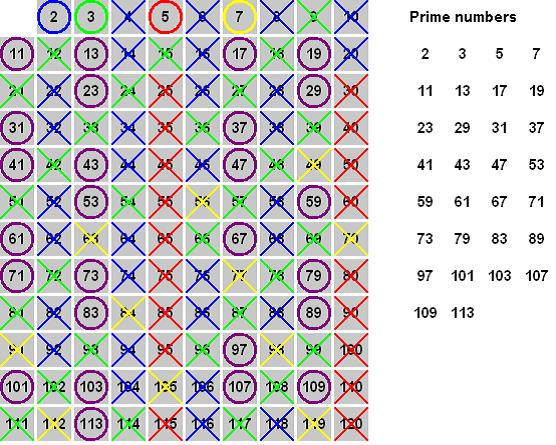
\includegraphics[width=0.75\textwidth,height=180pt]{1.jpg}
\end{figure}
\vspace*{-25pt}
\begin{center}
{\tiny{Image source:\url{http://commons.wikimedia.org/wiki/File:New_Animation_Sieve_of_Eratosthenes.gif}}
Used under the license given there}
\end{center}
\end{spacing}
\end{frame}
\begin{frame}[t,allowdisplaybreaks,allowframebreaks]{Euclid's Proof of the Infinity of the Number of Primes}
\begin{spacing}{1.05}
\begin{THEOREM}
There are infinitely many primes.\\[4pt]
\end{THEOREM}
\begin{PROOF}
Assume that there are only a finite number of primes, which we list as $p_1,\,...\,,p_n$. Set
\[Q=p_1\cdot p_2\cdots p_n+1.\]
By the Fundamental Theorem of Arithmetic, $Q$ is either prime or a product of primes. If $Q$ is prime, we have found a prime not in the list $p_1,\,...\,,p_n$. If $Q$ is not prime, then it has a prime factor, say $p_k$. Then $p_k\mid Q$ and $p_k\mid p_1\cdot p_2\cdots p_n$, so
\[p_k\mid\underbrace{(Q-p_1\cdot p_2\cdots p_n)},_{=1}\]
which is impossible. Therefore, there must be a prime not in the list.
\end{PROOF}
\newpage
\vspace*{8pt}
Note that the proof does \emph{not} state that $P_n=p_1\cdot p_2\cdots p_n+1$ must be a prime. However, it is interesting to note that it often seems to be the case:
\begin{itemize}
  \item $P_1=2+1=3$,
  \item $P_2=2\cdot3+1=7$,
  \item $P_3=2\cdot3\cdot5+1=31$,
  \item $P_4=2\cdot3\cdot5\cdot7+1=211$,
  \item $P_5=2\cdot3\cdot5\cdot7\cdot11+1=2311$,
  \item $P_6=2\cdot3\cdot5\cdot7\cdot11\cdot13+1=59\cdot509$ (not prime),
  \item $P_7=19\cdot97\cdot277$ (not prime), etc.
\end{itemize}
It is not known whether there are infinitely many $n$ for which $P_n$ is prime.
\end{spacing}
\end{frame}
\begin{frame}[t,allowdisplaybreaks,allowframebreaks]{Conjectures on Prime Numbers}
\begin{spacing}{1.1}
Prime numbers and their distribution among the integers have always
fascinated mathematicians. There are many conjectures that appear
simple, but have not yet been proven, or only partially proven, for example:\\[6pt]
\begin{itemize}
  \item The \emph{Twin Prime Conjecture} (antiquity): There are infinitely many primes $p$ such that $p+2$ is also prime. Such primes are called \emph{twin primes.}\\[4pt]
      The first hard result was obtained in May 2013, by Zhang Yitang, a
      Chinese-born Lecturer at the University of New Hampshire.\\[4pt]
      Zhang proved that there exists a number $k<70,\,000,\,000$ such that there are infinitely many prime pairs of the form $p,\,p+k$.\\[4pt]
      Subsequently, his methods were improved by many mathematicians to obtain the existence of a $k\leq246$. More details can be found, e.g., at\\[4pt]
      \url{http://www.wired.com/2013/11/prime/}
\newpage
  \item The \emph{Goldbach Conjecture} (1742): Every even number can be written as the sum of two prime numbers.\\[4pt]
      (It has been shown in 1995 that every even number is the sum of no more than 6 primes.)
  \item There are infinitely many primes of the form $p=n^2+1,\,n\in\N$.\\[4pt]
      (Remains unproven.)
  \item There are infinitely many primes of the form $p=4n+3,\,n\in\N$.\\[4pt]
      (See assignments.)
  \item For fixed $a,b\in\N$ with $\gcd(a,b)=1$, there are infinitely many primes of the form $p=an+b,\,n\in\N$.\\[4pt]
      (This is Dirichlet's Theorem, established in 1837.)
\end{itemize}
\end{spacing}
\end{frame}
\subsection{The Theory of Congruences}
\begin{frame}[c] \begin{spacing}{2}
\tableofcontents[sectionstyle=hide,subsectionstyle=show/shaded/hide]
\end{spacing}
\end{frame}
\begin{frame}[t,allowdisplaybreaks,allowframebreaks]{Congruency}
\begin{spacing}{1}
\begin{DEFINITION}
For $a,b\in\Z$ and $m\in\N\setminus\{0\}$ we say that $a$ \emph{is congruent to $b$ modulo $m$}, writing
\[a\equiv b\,(\text{mod}\, m)\qquad\quad
\text{if and only if}\qquad\quad
m\mid(a-b).\]
\end{DEFINITION}
\!\!\begin{LEMMA}
Let $a,b\in\Z$ and $m\in\N\setminus\{0\}$. Then
\[a\equiv b\,(\text{mod}\,m)\quad
\Leftrightarrow\quad\mathop{\exists}_{k\in\Z}
a=b+km.\]
\end{LEMMA}
\begin{PROOF}
\begin{equation*}
  \begin{split}
     a\equiv b\,(\text{mod}\,m)\quad &\Leftrightarrow\quad m\mid(a-b)\quad\Leftrightarrow\quad
     \mathop{\exists}_{k\in\Z}a-b=km \\
       &\Leftrightarrow\quad\mathop{\exists}_{k\in\Z}
       a=b+km
  \end{split}
\end{equation*}
\end{PROOF}
\newpage
Given $m\in\N\setminus\{0\}$, by the division algorithm, for every $a\in\Z$ there exist unique $q,r$ such that
\[a=q\cdot m+r,\qquad\qquad\qquad
0\leq r<m.\]
We write
\[q=:a\,\,\text{div}\,m,\qquad\qquad\qquad
r=:a\,\,\text{mod}\,m.\]
for the quotient $q$ and the remainder $r$ modulo $m$.\\[4pt]
Lemma 1.8.2 can then be expressed as follows:\\[6pt]
\begin{THEOREM}
Let $a,b\in\Z$ and $m\in\N\setminus\{0\}$. Then
\[a\equiv b\quad(\text{mod}\,m)\quad
\Leftrightarrow\quad a\,\,\text{mod}\,\,m=b\,\,\text{mod}\,\,m\]
\end{THEOREM}
\!Hence, two numbers are congruent modulo $m$ if and only if they have the
same remainder modulo $m$.
\end{spacing}
\end{frame}
\begin{frame}[t,allowdisplaybreaks,allowframebreaks]{Congruence Classes}
\begin{spacing}{1.1}
The congruence (mod $m$) is an equivalence relation on $\Z$:
\setcounter{equation}{0}
\begin{equation}\label{1.8.1}
a\sim b\qquad\quad\Leftrightarrow\qquad\quad
a\equiv b\,(\text{mod}\,\,m)
\end{equation}
is reflexive, symmetric and transitive.\\[4pt]
By Theorem 1.4.7 every equivalence relation induces a partition of the underlying set.\\[4pt]
\begin{DEFINITION}
The partition on the integers induced by the congruency
relation of Definition 1.8.1 is denoted by $\Z_m$. The fibers (equivalence classes) of this partition are called \emph{congruence classes}. We write
\[\Z_m=\{[0]_m,[1]_m,\,...\,,[m-1]_m\}\]
\end{DEFINITION}
\end{spacing}
\newpage
\begin{spacing}{1}
Hence, a single equivalence class $[a]_m$ contains all integers that have the same remainder when divided by $m$.\\[4pt]
\begin{EXAMPLE}
For $m=2$ the relation \eqref{1.8.1} induces the partition
\[\Z_2=\{[0]_2,[1]_2\}\]
where the two classes contain the even and odd numbers, respectively. See also Example 1.4.5 and 1.6.4.\\[4pt]
\end{EXAMPLE}
\stepcounter{zhuo}
\alert{1.8.6. Definition and Theorem.} The partition $\Z_m$ together with addition and multiplication defined by
\[[a]_m+[b]_m:=[a+b]_m,\qquad\qquad\quad
[a]_m\cdot[b]_m:=[a\cdot b]_m\]
defines a commutative ring. We usually drop the equivalence class
notation and simply write
\[\Z_m=\{0,\,1,\,...\,,m-1\}\]
\end{spacing}
\newpage
\begin{spacing}{1.1}
The well-definedness of addition and multiplication follows from the following lemma:\\[4pt]
\begin{LEMMA}
Let $a,b,c,d\in\Z$ and $m\in\N\setminus\{0\}$. If $a\equiv b\,(\text{mod}\,m)$ and $c\equiv d\,(\text{mod}\,m)$ then
\[a+c\,\equiv\,b+d\,(\text{mod}\,m)\qquad\quad
\text{and}\qquad\quad ac\,\equiv\,bd\,(\text{mod}\,m).\]
\end{LEMMA}
\begin{PROOF}
By Lemma 1.8.2 there exist $s,t\in\Z$ such that $b=a+sm,\,d=c+tm$. Then
\[b+d=a+c+m(s+t)\qquad\quad\Leftrightarrow
\qquad\quad a+c\,\equiv\,b+d~\text{mod}\,m\]
and
\[bd=ac+m(at+cs+stm)\qquad\quad
\Leftrightarrow\qquad\quad
ac\,\equiv\,bd\,\text{mod}\,m.\]
\end{PROOF}
\end{spacing}
\end{frame}
\begin{frame}[t,allowdisplaybreaks,allowframebreaks]{Modular Arithmetic}
\begin{spacing}{1.1}
The ring properties of $\Z_p$ are left for you to prove.\\[5pt]
As a corollary of Lemma 1.8.7 we obtain\\[4pt]
\begin{COROLLARY}
Let $a,b\in\Z$ and $m\in\N\setminus\{0\}$. Then
\begin{align*}
  a+b &\equiv\big(a\:\text{mod}\:m+b\:\text{mod}\:m\big)~
  (\text{mod}\:m) \\
  ab &\equiv\big((a\:\text{mod}\:m)(b\:\text{mod}\:m)\big)~
  (\text{mod}\:m).
\end{align*}
\end{COROLLARY}
Hence, to find the product (sum) of two numbers modulo $m$, it suffices to
multiply (add) their remainders (modulo $m$). This is the basis of \emph{modular
arithmetic}, a very fruitful field of number theory.
\newpage
\vspace*{12pt}
\begin{EXAMPLE}
We prove that $41\mid 2^{20}-1$. This is equivalent to showing that
\[2^{20}-1\equiv0\enskip(\text{mod}\,41).\]
We note that $2^5-32\equiv-9\,(\text{mod}\,41)$. Then Corollary 1.8.8 implies
\[2^{20}=(2^5)^4\equiv(-9)^4\enskip
(\text{mod}\,41)\]
But $(-9)^4=81\cdot81$ and $81\equiv-1\,(\text{mod}\,41)$. Again by Corollary 1.8.8,
\[2^{20}\equiv(-1)^2\equiv1~(\text{mod}\,41)\]
from which the assertion follows.
\end{EXAMPLE}
\newpage
\vspace*{12pt}
\begin{EXAMPLE}
We calculate the remainder
\[(1!+2!+3!+4!+\cdots+100!)\,\text{mod}\,12.\]
Since $4!=2\cdot12$, we have $12\mid n!$ for all $n\geq4$. This implies
\begin{equation*}
  \begin{split}
       &~~~~(1!+2!+3!+4!+\cdots+100!)\,\text{mod}\,12  \\
       &=1!\,\text{mod}\,12+2!\,\text{mod}\,12+3!\,\text{mod}\,12
       +\underbrace{4!\,\text{mod}\,12}_{=0}+\cdots+
       +\underbrace{100!\,\text{mod}\,12}_{=0}  \\
       &=1+2+6=9.
  \end{split}
\end{equation*}
\end{EXAMPLE}
\end{spacing}
\end{frame}
\begin{frame}[t,allowdisplaybreaks,allowframebreaks]{Division in Modular Arithmetic}
\begin{spacing}{1.1}
\vspace*{10pt}
We have seen that for any integers $a,b,c\in\Z$ and $m\in\N\setminus\{0\}$
\[a\equiv b\quad(\text{mod}\,m)\]
implies
\[ac\equiv bc\quad(\text{mod}\,m).\]
However, the converse is not necessarily true:
\[2\cdot1\equiv 2\cdot4~(\text{mod}\,6)\quad\quad
\text{but}\qquad\qquad1\not\equiv4~(\text{mod}\,6).\]
The next theorem gives the correct way to divide in modular arithmetic.
\newpage
\begin{THEOREM}
Let $a,b,c\in\Z$ and $m\in\N\setminus\{0\}$. Then
\[ac\equiv bc\quad(\text{mod}\,m).\]
implies
\[a\equiv b\quad(\text{mod}\,m/d)\]
where $d=\gcd(c,m)$.\\[4pt]
\end{THEOREM}
\begin{PROOF}
We have
\[ac-bc=k\cdot m\qquad\qquad\qquad
\text{for some}~k\in\Z.\]
There exist integers $r,s$ with $\gcd(r,s)=1$ such that $c=rd,\,m=sd$. Inserting into the equation,
\[ard-brd=k\cdot sd\]
\newpage
\alert{Proof (continued).}\\
Canceling the common factor $d$,
\[r(a-b)=ks.\]
so $s\mid r(a-b)$. Since $\gcd(r,s)=1$, Euclid's Lemma gives $s\mid (a-b)$. Hence,
\[a\equiv b\enskip\text{mod}\,s.\]
Since $s=m/d$, we are finished.
\end{PROOF}
\begin{COROLLARY}
Let $a,b,c\in\Z$ and $m\in\N\setminus\{0\}$ and $\gcd(c,m)=1$. Then
\[ac\equiv bc\quad(\text{mod}\,m).\]
implies
\[a\equiv b\quad(\text{mod}\,m)\]
\end{COROLLARY}
\newpage
\vspace*{13pt}
\begin{COROLLARY}
Let $a,b,\in\Z$ and $p\in\N\setminus\{0\}$ a prime number. Then
\[ac\equiv bc\quad(\text{mod}\,p).\]
implies
\[a\equiv b\quad(\text{mod}\,p)\]
for any $c\in\Z\setminus\{0\}$.\\[4pt]
\end{COROLLARY}
Corollary 1.8.13 can be used to prove that $\Z_p$ is an integral domain if $p$ is prime. In fact, a much stronger result holds.
\end{spacing}
\end{frame}
\begin{frame}[c,allowdisplaybreaks,allowframebreaks]{Congruence Classes as Fields}
\begin{spacing}{1.1}
\begin{THEOREM}
The partition $\Z_p$ is a field if and only if $p$ is a prime number.\\[4pt]
\end{THEOREM}
\begin{PROOF}
\begin{itemize}
  \item[($\Leftarrow$)] By Definition 1.8.6, $\Z_p$ is a commutative ring. Therefore $(\Z_p,+)$ is a group and for $(\Z_p,\cdot)$ to also be a group we only need to prove that for any $a\neq0$ there exists $b\in\Z_p$ such that $a\cdot b=1$.\\[4pt]
      Let $a\in\Z_p\setminus\{0\}$. Since $p$ is prime it is relatively prime to any other number, including $a$. Then B\'{e}zout's lemma states that there exist $x,y\in\Z$ such that
      \[a\cdot x+p\cdot y=1.\]
      This implies
      \[a\cdot x\equiv 1\quad(\text{mod}\,p)\]
      and $x$ is the multiplicative inverse of $a$ modulo $p$.
\end{itemize}
\newpage
\alert{Proof (continued).}\\[4pt]
\begin{itemize}
  \item[($\Rightarrow$)] Suppose that $p$ is not prime. Then there exist $a,b\in\Z$ with $1<a,b<p$ such that $p=a\cdot b$. If $\Z_p$ is a field, then by definition $a$ must have a multiplicative inverse $a^{-1}$ such that $a\cdot a^{-1}=1$. Thus we can write:
      \[b\cdot1=b\cdot(a\cdot a^{-1})=(b\cdot a)\cdot a^{-1}=p\cdot a^{-1}\equiv0\,(\text{mod}\,p)\]
      This contradicts $b\notin\{0,p\}$. Hence. $a$ does not have a multiplicative inverse and $\Z_p$ is not a field.
\end{itemize}
\end{PROOF}
\end{spacing}
\end{frame}
\begin{frame}[c]{Linear Congruences}
\begin{spacing}{1.1}
\begin{DEFINITION}
Let $a,b\in\Z$ and $m\in\N\setminus\{0\}$. A \emph{linear congruence} is an equation
\begin{equation}\label{1.8.2}
ax\equiv b\enskip\text{mod}\,m
\end{equation}
for unknowns $x\in\Z$.\\[4pt]
\end{DEFINITION}
We are interested in finding all $x\in\Z$ that satisfy \eqref{1.8.2}, up to congruency modulo $m$.\\[4pt]
Note that \eqref{1.8.2} can be rephrased as
\begin{equation}\label{1.8.3}
ax-my=b,
\end{equation}
which is simply the linear diophantine equation \eqref{1.6.4}. Hence, we can
base our theory of solvability on known results for the diophantine
equation.
\end{spacing}
\end{frame}
\begin{frame}[t,allowdisplaybreaks,allowframebreaks]{Solvability of Linear Congruences}
\begin{spacing}{1.1}
\begin{THEOREM}
Let $a,b\in\Z$ and $m\in\N\setminus\{0\}$ and $d=\gcd(a,m)$. The linear congruence $ax\equiv b\enskip\text{mod}\,m$ has a solution if and only if $d\mid b$. In that case, it has $d$ solutions that are mutually incongruent modulo $m$.\\[5pt]
\end{THEOREM}
\begin{PROOF}
We already know from Theorem 1.6.26 that \eqref{1.8.3} has a solution if and only if $d\mid m$, so the same is true of \eqref{1.8.2}.\\[4pt]
If a solution $(x_0,y_0)$ exists, all other solutions of \eqref{1.8.3} are given by
\[x=x_0+\frac{m}{d}t,\qquad\qquad
y=y_0+\frac{m}{d}t,\qquad\qquad
t\in\Z.\]
Suppose $t=0,\,...\,,d-1$. We claim that these solutions are mutually
incongruent, while all other solutions are congruent modulo $m$.
\newpage
\vspace*{5pt}
\alert{Proof (continued).}\\
Suppose first that
\[x_0+\frac{m}{d}t_1\equiv x_0+\frac{m}{d}t_2~(\text{mod}\,m),\qquad\quad
0\leq t_1<t_2\leq d-1.\]
Then
\[\frac{m}{d}t_1\equiv\frac{m}{d}t_2\,(\text{mod}\,m),\]
Since $\gcd(m/d,m)=m/d$ by Theorem 1.8.11 we can cancel the factor $m/d$ to obtain
\[t_1\equiv t_2\enskip(\text{mod}\,d).\]
But this contradicts $0\leq t_1<t_2\leq d-1$. Hence, the solutions for $t=0,\,...\,,d-1$ are mutually incongruent.
\newpage
\alert{Proof (continued).}\\
Finally, we show that any other solution is congruent to one of the $d$ solutions with $t=0,\,...\,,d-1$. Suppose an arbitrary $t\in\Z$ is given. By the Division Algorithm, there exist $q,r\in\Z$ such that
\[t=qd+r,\qquad\qquad\qquad0\leq r\leq d-1.\]
Then
\begin{equation*}
  \begin{split}
     x_0+\frac{m}{d}t &=x_0+\frac{m}{d}(qd+r) \\
       &=x_0+mq+\frac{m}{d}r \\
       &=x_0+\frac{m}{d}r\,(\text{mod}\,m),
  \end{split}
\end{equation*}
so the solution is congruent to some solution with $t=0,\,...\,,d-1$.
\end{PROOF}
\end{spacing}
\end{frame}
\begin{frame}[t,allowdisplaybreaks,allowframebreaks]{Solving Linear Congruences}
\begin{spacing}{1.05}
\begin{EXAMPLE}
We solve the linear congruence
\[18x\equiv30\enskip(\text{mod}\,42).\]
Since $\gcd(18,42)=6$ and $6\mid 30$ there are exactly 6 mutually incongruent solutions. We guess a particular solution $x=4$. Then the other incongruent solutions are given by
\[x=4+\frac{42}{6}t=4+7t,\qquad\qquad\quad
t=0,\,...\,,5.\]
or
\[x_0=4,\quad x_1=11,\quad x_2=18,\quad x_3=25,\quad x_4=32,\quad x_5=39\]
But how do we find this first solution $x = 4$ systematically, without
resorting to guessing?
\end{EXAMPLE}
\end{spacing}
\newpage
\begin{spacing}{1}
We use the following consequence of Theorem 1.8.16,\\[4pt]
\begin{COROLLARY}
Let $a,b\in\Z$ and $m\in\N\setminus\{0\}$ and $\gcd(a,m)=1$. Then the linear congruence $ax\equiv b~\text{mod}\,m$ has a unique solution modulo $m$.\\[4pt]
\end{COROLLARY}
\begin{EXAMPLE}
We first attempt to reduce the problem
\[18x\equiv 30\enskip(\text{mod}\,42).\]
to one which has a unique solution. We divide by $\gcd(18,42)=6$, giving
\[3x\equiv 5\enskip(\text{mod}\,7).\]
Again, at this point we might guess (more easily than before) $x=4$ and find the other solutions
\[x_0=4,\quad x_1=11,\quad x_2=18,\quad x_3=25,\quad x_4=32,\quad x_5=39\]
which are all congruent modulo 7 but incongruent modulo 42.
\end{EXAMPLE}
\end{spacing}
\end{frame}
\begin{frame}[t,allowdisplaybreaks,allowframebreaks]{Modular Inverse}
\begin{spacing}{1.1}
\vspace*{10pt}
But the basic problem remains: How to find the initial solution to a
congruence?\\[5pt]
One method (apart from guessing) is based on the following concept.\\[4pt]
\begin{DEFINITION}
Let $a\in\Z$ and $m\in\N\setminus\{0,1\}$ be given. Then an integer $\widetilde{a}\in\Z$ such that
\[a\widetilde{a}\equiv1\enskip(\text{mod}\,m).\]
is said to be an \emph{inverse of a modulo $m$}.\\[5pt]
\end{DEFINITION}
\begin{THEOREM}
Let $a\in\N\setminus\{0\}$ and $m\in\N\setminus\{0,1\}$. If $\gcd(a,m)=1$, the inverse of $a$ modulo $m$ exists. This inverse is unique modulo $m$.
\end{THEOREM}
\end{spacing}
\newpage
\begin{spacing}{1.05}
\vspace*{10pt}
\begin{PROOF}
By B\'{e}zout's Lemma 1.6.10 there exist $s,t\in\Z$ such that $sa+tm=1$. This means, in particular, that
\[sa+tm\equiv1\enskip(\text{mod}\,m).\]
Then
\begin{equation}\label{1.8.4}
 sa\equiv1\,(\text{mod}\,m)
\end{equation}
and $s$ is the inverse of $a$ modulo $m$. Therefore, the modular inverse of $a$ exists.
\newpage
\alert{Proof (continued).}\\
Now suppose $a'$ and $\widetilde{a}$ are two modular inverses of $a$. Then
\[a\widetilde{a}\equiv1\equiv aa'\enskip(\text{mod}\,m).\]
so
\[a(\widetilde{a}-a')\equiv0\enskip(\text{mod}\,m).\]
Since $\gcd(a,m)=1$, Corollary 1.8.12 allows us to divide by $a$ to obtain
\[a'\equiv\widetilde{a}\enskip(\text{mod}\,m).\]
\end{PROOF}
\begin{REMARK}
The proof of Theorem 1.8.21 also yields a method for
finding an inverse of $a$ modulo $m$: find (by using the Euclidean algorithm)
a linear combination of $a$ and $m$ that equals 1. The coefficient of $a$ will be
an inverse of $a$ modulo $m$.
\end{REMARK}
\end{spacing}
\end{frame}
\begin{frame}[c,allowdisplaybreaks,allowframebreaks]{Solving Congruencies using the Modular Inverse}
\begin{spacing}{1}
Once we have found the inverse, we can easily solve a congruence by
multiplying both sides with the inverse.\\[4pt]
\begin{EXAMPLE}
We want to solve the congruence $3x\equiv5~(\text{mod}\,7)$. We first find an inverse of $3\:\text{mod}\:7$. Applying the Euclidean algorithm,
\begin{align*}
  3 &=1\cdot7-4, \\
  7 &=(-1)\cdot(-4)+3, \\
  -4 &=(-1)\cdot3-1, \\
  3 &=(-3)\cdot1+0,
\end{align*}
so $\gcd(3,7)=1$, as expected and
\begin{equation*}
  \begin{split}
     1 &=(-1)\cdot3+4 \\
       &=(-1)\cdot3+(7-3) \\
       &=(-2)\cdot3+7.
  \end{split}
\end{equation*}
It follows that an inverse of $a=3$ modular 7 is $\widetilde{a}=-2$.
\end{EXAMPLE}
\newpage
We then multiply the congruency
\[3x\equiv 5\enskip(\text{mod}\,7)\]
by $\widetilde{a}=-2$, obtaining
\[-6x\equiv -10\enskip(\text{mod}\,7)\]
Since $-6\equiv1~(\text{mod}\,7)$ and $-10\equiv4\,(\text{mod}\,7)$, we obtain
\[1\cdot x\equiv4\enskip(\text{mod}\,7),\]
as expected.
\end{spacing}
\end{frame}
\begin{frame}[t]{Sunzi's Problem}
\begin{spacing}{1.1}
The Chinese Remainder theorem is based on a problem posed by the
Chinese mathematician Sunzi (孫子/ 孙子) and published in his book
``孫子算經'' (perhaps best translated as ``Master Sun's Mathematical
Manual'') in the first or third century AD (dates by: Rosen's book and
wikipedia, respectively.)\\[5pt]
Sunzi asks:\\[5pt]
\begin{quote}
There are certain things whose number is unknown. When
divided by 3, the remainder is 2; when divided by 5, the
remainder is 3; and when divided by 7, the remainder is 2. What
will be the number of things?
\end{quote}
\begin{center}
今有物不知其数,三三数之剩二,五五数之剩三,\\
七七数之剩二,问物几何?
\end{center}
\end{spacing}
\end{frame}
\begin{frame}[t,allowdisplaybreaks,allowframebreaks]{The Chinese Remainder Theorem}
\begin{spacing}{1}
Sunzi's problem can be written in modern mathematical notation as a system of congruences,
\begin{align*}
  x &\equiv2\:(\text{mod}\,3),  \\
  x &\equiv3\:(\text{mod}\,5),  \\
  x &\equiv2\:(\text{mod}\,7).
\end{align*}
\stepcounter{zhuo}
\alert{1.8.24. Chinese Remainder Theorem.} Let $m_1,\,...\,,m_n\in\N\setminus\{0\}$ be pairwise relatively prime and $a_1,\,...\,,a_n\in\Z$. Then the system of congruences
\begin{equation}\label{1.8.5}
\begin{aligned}
  x &\equiv a_1\:(\text{mod}\,m_1), \\
  x &\equiv a_2\:(\text{mod}\,m_2), \\
    &\vdots \\
  x &\equiv a_n\:(\text{mod}\,m_n).
\end{aligned}
\end{equation}
has a unique solution modulo $m=m_1m_2\,...\,m_n$.
\newpage
\begin{PROOF}
We first show the existence of a solution by demonstrating how to construct it. Let
\[M_k:=\frac{m}{m_k}=\prod_{i\neq k}m_i.\]
Then $\gcd(m_k,M_k)=1$ and by Theorem 1.8.21 there exists an inverse $y_k$ to $M_k$ modulo $m_k$, i.e.,
\[M_ky_k\equiv1\enskip(\text{mod}\,m_k),\]
Then it is easily verified that
\[x=\sum_{k=1}^{n}a_kM_ky_k\]
is a solution to \eqref{1.8.5} (noting that $M_j\equiv0~\text{mod}\,m_i$ for $i\neq j$).
\newpage
\alert{Proof (continued).}\\
Now suppose there are two solutions $x,x'$ to the system of congruences. Then for $k=1,\,...\,,n,$
\[x\equiv a_k\equiv x'\enskip(\text{mod}\,m_k).\]
This implies
\[m_k\mid(x-x')\qquad\qquad\qquad
k=1,\,...\,,n.\]
Since $\gcd(m_k,m_j)=1$ for all $j,k=1,\,...\,,n$, Corollary 1.6.16 allows us to deduce
\[\underbrace{m_1\cdots m_n}_{=m}\mid(x-x')\]
which proves uniqueness modulo $m$.
\end{PROOF}
\end{spacing}
\end{frame}
\begin{frame}[t]{Solution to Sunzi's Problem}
\begin{spacing}{1.1}
To find the answer to Sunzi's original question, set\\[4pt]
$m=m_1m_2m_3=3\cdot 5\cdot 7=105$. Then
\[M_1=m/3=35,\qquad\quad M_2=m/5=21,\qquad\quad M_3=m/7=15.\]
We then find the inverse of $M_k\mod m_k$,
\[y_1=2,\qquad\qquad y_2=1,\qquad\qquad
y_3=1.\]
The solution to the system is then
\[x=2\cdot35\cdot2+3\cdot21\cdot1+2\cdot15\cdot1=233
\equiv23\enskip(\text{mod}\,105).\]
Thus 23 is the smallest integer that satisfies Sunzi's problem, but the solution is only unique modulo 105.
\end{spacing}
\end{frame}
\begin{frame}[t,allowdisplaybreaks,allowframebreaks]{Solution of a System in an Elementary Fashion}
\begin{spacing}{0.85}
\begin{EXAMPLE}
We solve the congruency
\[17x\equiv9\enspace(\text{mod}\,276).\]
Instead of solving it directly, we note that $276=3\cdot4\cdot23$, so the congruency is equivalent to the system
\[17x\equiv9\,(\text{mod}\,3),\qquad\quad
17x\equiv9\,(\text{mod}\,4),\qquad\quad
17x\equiv9\,(\text{mod}\,23).\]
(Why?) We can simplify this system to
\[x\equiv0\,(\text{mod}\,3),\qquad\quad
x\equiv1\,(\text{mod}\,4),\qquad\quad
17x\equiv9\,(\text{mod}\,23).\]
(Why?)\\[2pt]
The first congruence gives $x=3k,\,k\in\Z$. Substituting into the second congruence,
\[3k\equiv1\enspace(\text{mod}\,4)\]
The modular inverse of $a=3$ is $\widetilde{a}=3$, so we obtain
\[k\equiv3\enspace(\text{mod}\,4)\]
\end{EXAMPLE}
\end{spacing}
\begin{spacing}{1}
We then have
\[x=3\cdot(3+4j)=9+12j,\qquad\qquad\qquad
j\in\Z.\]
Inserting into the last congruence,
\[17\cdot(9+12j)\equiv9\enskip(\text{mod}\,23)\]
or
\[204j\equiv-144\enskip(\text{mod}\,23).\]
This reduces to $3j\equiv6~(\text{mod}\,23)$. Hence, $j=2+23t,\,t\in\Z$ and hence
\[x=33+276t\]
or simply $x\equiv33~(\text{mod}\,276)$.
\end{spacing}
\end{frame}
\subsection{Factorization and Verifying Primality}
\begin{frame}[c] \begin{spacing}{2}
\tableofcontents[sectionstyle=hide,subsectionstyle=show/shaded/hide]
\end{spacing}
\end{frame}
\begin{frame}[t,allowdisplaybreaks,allowframebreaks]{Fermat's Factorization Method}
\begin{spacing}{1.1}
One of the most important problems in number theory is the finding of
factors of a composite number, or of determining that a number is prime.\\[5pt]
The basic algorithm from antiquity is the Sieve of Eratosthenes, which is
based on Theorem 1.7.7:\\[5pt]
\begin{quote}
To find factors (if any exist) of a number $n$, one tests all primes less than $\sqrt{n}$ to see if they divide $n$.
\end{quote}
Eratosthenes lived around 200 B.C. - it took until 1643, 1800 years later,
for a significant improvement on this algorithm to be found. In that year,
Pierre de Fermat formulated the following idea in a letter to Mersenne:\\[4pt]
\begin{quote}
Finding two factors of an odd number $n$ is equivalent to solving the quadratic, two-variable Diophantine equation $n=x^2-y^2$.
\end{quote}
\newpage
This is easy to see, because if $x$ and $y$ satisfy $n=x^2-y^2$, then
\[n=x^2-y^2=(x+y)(x-y)\]
and $x\pm y$ are factors of $n$. On the other hand, if $n=ab$ and $n$ is odd, then
\[n=\left(\frac{a+b}{2}\right)^2-\left(\frac{a-b}{2}\right)^2\]
and $(a\pm b)/2$ are solutions to the Diophantine equation. (Note that if odd, then so are $a$ and $b$, so $a\pm b$ is even.)\\[5pt]
Therefore, finding $a$ and $b$ such that $n=ab$ is accomplished by finding $x$ and $y$ such that
\[x^2-n=y^2\]
\newpage
We proceed as follows:
\begin{itemize}
  \item Find the smallest $k$ such that $k^2>n$.
  \item Consider successively the numbers
      \[k^2-n,\qquad\qquad (k+1)^2-n,\qquad\qquad
      (k+2)^2-n,\,...\]
      until one of these numbers is a square.
  \item The process must terminate, since
      \[\left(\frac{n+1}{2}\right)^2-n=\left(\frac{n-1}{2}\right)^2\]
      which corresponds to the trivial factorization $n=1\cdot n$.
\end{itemize}
\newpage
\begin{EXAMPLE}
We apply the method to the number $n=119143$. By any available means, we find
\[345^2<119143<346^2.\]
We need to calculate $k^2-119143$ for
\[346<k<\frac{119143+1}{2}=59572.\]
We find:
\begin{align*}
  &346^2-119143=573, \qquad\qquad\qquad~~
  347^2-119143=1266, \\
  &348^2-119143=1961, \qquad\qquad\qquad 349^2-119143=2658, \\
  &350^2-119143=3357, \qquad\qquad\qquad 351^2-119143=4058, \\
  &352^2-119143=4761=69^2.
\end{align*}
Hence, $119143=(352+69)(352-69)=421\cdot283$.
\end{EXAMPLE}
\end{spacing}
\end{frame}
\begin{frame}[c]{Finding Squares}
\begin{spacing}{1.1}
For using this method, it is useful to note that
\begin{itemize}
  \item Square numbers must end in one of the digits $0,1,4,5,6,9$.
  \item By calculating $k^2\,\text{mod}\,100$ for $0\leq k\leq 99$, the last two digits must be one of the following:\\[3pt]
      \[\begin{array}{l@{\hspace{21pt}}l@{\hspace{21pt}}l@{\hspace{21pt}}l@{\hspace{21pt}}c}
        0 & 1 & 4 & 9 & 16 \\[2pt]
        21 & 24 & 25 & 29 & 36 \\[2pt]
        41 & 44 & 49 & 56 & 61 \\[2pt]
        64 & 69 & 76 & 81 & 84 \\[2pt]
        89 & 96 &   &  &
      \end{array}\]
\end{itemize}
In the previous example, this means we need only actually test the numbers 1961 and 4761 for being squares.
\end{spacing}
\end{frame}
\begin{frame}[t,allowdisplaybreaks,allowframebreaks]{Fermat's Little Theorem}
\begin{spacing}{1.1}
Fermat wrote extensively on prime numbers; one of his most important
results is called his ``little'' theorem, to distinguish it from his ``last'' theorem, that for $n\geq3$ the equation $x^n+y^n=z^n$ has no integer solutions $x,y,z$.\\[5pt]
\stepcounter{zhuo}
\alert{1.9.2. Fermat's Little Theorem.} Let $p\in\N$ and $a\in\N$. If $p$ is prime and $p\nmid a$, then
\setcounter{equation}{0}
\begin{equation}\label{1.9.1}
a^{p-1}\equiv1~(\text{mod}~p).
\end{equation}
More generally, for any prime $p\in\N$ and $a\in\Z$,
\begin{equation}\label{1.9.2}
a^p\equiv a~(\text{mod}~p).
\end{equation}
\newpage
\begin{PROOF}
Consider the $p-1$ numbers
\begin{equation}\label{1.9.3}
a,\qquad 2a,\qquad 3a,\quad\quad...,\qquad(p-1)a
\end{equation}
Since $\gcd(p,a)=1$, these numbers are incongruent modulo $p$:
\[ra\equiv sa\quad(\text{mod}\,p)\]
implies $r\equiv s\,(\text{mod}\:p)$ for any $r,s\in\Z$. Therefore, the integers \eqref{1.9.3} must each be congruent to one of the numbers $1,2,3,\,...\,,p-1$, in some order. Hence,
\[a\cdot 2a\cdot 3a\cdots(p-1)a\equiv (p-1)!\enskip(\text{mod}\,p).\]
Canceling $(p-1)!$ on both sides (why can we do this), we obtain \eqref{1.9.1}.
\newpage
\alert{Proof (continued).}\\
The statement \eqref{1.9.2} is trivially true if $p\mid a$: then $a\equiv0\equiv a^p~(\text{mod}\,p)$. If $p\nmid a$, we simply multiply \eqref{1.9.1} by $a$ to obtain \eqref{1.9.2}.
\end{PROOF}
\vspace*{16pt}
\begin{EXAMPLE}
We calculate $5^{38}~\text{mod}\,11$. By Fermat's Little Theorem,
\[5^10=5^{11-1}\equiv1\enskip(\text{mod}\,11).\]
Then
\begin{equation*}
  \begin{split}
     5^{38} &=5^{10\cdot3+8}=(5^{10})^3(5^2)^4 \\
       &\equiv1^3\cdot3^4\equiv 821\equiv4\,(\text{mod}\,11).
  \end{split}
\end{equation*}
\end{EXAMPLE}
\newpage
Another application is to show that a number $n$ is not prime: if for some $a\in\N\setminus\{0\}$
\[a^n\not\equiv a\enskip(\text{mod}\:n),\]
then $n$ can not be prime.\\[5pt]
\begin{EXAMPLE}
Consider $n=117$. Then
\begin{equation*}
  \begin{split}
     2^{117} &=(2^7)^{16}2^5 \\
       &=128^{16}2^5 \\
       &\equiv11^{16}2^5\equiv 121^82^5\equiv4^82^5~(\text{mod}\,117) \\
       &\equiv2^{21}\equiv(2^7)^3\equiv11^3\equiv
       4\cdot11\equiv44\,(\text{mod}\,117) \\
       &\not\equiv2\,(\text{mod}\,117),
  \end{split}
\end{equation*}
so 117 is not prime. In fact, $117=13\cdot9$.
\end{EXAMPLE}
\end{spacing}
\end{frame}
\begin{frame}[t,allowdisplaybreaks,allowframebreaks]{Fermat Pseudoprimes}
\begin{spacing}{1.1}
We know that if $p$ is prime, then
\[a^{p-1}\equiv1\enskip(\text{mod}\,p)\]
for any $a$ with $p\nmid a$. But is the converse true? If the congruence holds, must $p$ be prime?\\[5pt]
We claim that this is not the case. In fact, we will show that
\[2^{341}-1\equiv1\enskip(\text{mod}\,341)\]
but $341=11\cdot31$ is not prime.\\[5pt]
In fact, composite numbers for which $a^{p-1}\equiv1~(\text{mod}\,p)$ are called \emph{Fermat pseudoprimes to base $a$}.
\end{spacing}
\newpage
\begin{spacing}{0.9}
To verify our assertion that 341 is a Fermat pseudoprime to base 2, we need a technical result:\\[5pt]
\begin{LEMMA}
Let $p,q\in\N\setminus\{0\}$ be prime numbers such that
\[a^p\equiv a\,(\text{mod}\,q)\qquad\qquad
\text{and}\qquad\qquad a^q\equiv a\,(\text{mod}\,p)\]
then
\[a^{pq}\equiv a~\,(\text{mod}\,pq).\]
\end{LEMMA}
\begin{PROOF}
By \eqref{1.9.2},
\[(a^q)^p\equiv a^q\enskip(\text{mod}\,p).\]
By assumption, $a^q\equiv a\,(\text{mod}\,p)$. Thus,
\[a^{pq}\equiv a\,(\text{mod}\,p)\qquad\qquad
\text{or}\qquad\qquad p\mid(a^{pq}-a).\]
Similarly, $q\mid(a^{pq}-a)$, so $pq\mid(a^{pq}-a)$ since $\gcd(p,q)=1$.
\end{PROOF}
\end{spacing}
\newpage
\begin{spacing}{1.05}
We now show that $2^{340}\equiv1\,(\text{mod}\,341)$ where $341=11\cdot31$. First, note that
\[2^{10}=1024=31\cdot33+1\]
so
\[2^{11}=2\cdot2^{10}\equiv2\cdot1\equiv2\enskip
(\text{mod}\,31)\]
and
\[2^{31}=2(2^{10})^3\equiv2\cdot1^3\equiv2\enskip
(\text{mod}\,11).\]
By Lemma 1.9.5,
\[2^{341}=2^{11\cdot31}\equiv2\enskip(\text{mod}\,341).\]
Canceling the factor 2,
\[2^{340}\equiv1\enskip(\text{mod}\,341).\]
\end{spacing}
\end{frame}
\begin{frame}[t,allowdisplaybreaks,allowframebreaks]{Wilson's Theorem}
\begin{spacing}{1.05}
Finally, we give another result on prime numbers, dating from the late 18\textsuperscript{th} century.\\[5pt]
\alert{1.9.6. Wilson's Theorem.} Let $p\in\N$ be prime. Then
\[(p-1)!\equiv-1\enskip(\text{mod}\,p).\]
\begin{PROOF}
The cases $p=2$ and $p=3$ are obvious, so we suppose $p>3$. Let $a$ be any of the numbers
\[1,2,3,\,...\,,p-1.\]
Then, by Theorem 1.8.21, the inverse $\widetilde{a}$ modulo $p$ of $a$ exists and is unique modulo $p$
\[\widetilde{a}a\equiv1\enskip(\text{mod}\,p).\]
We first show that $a=\widetilde{a}$ if and only if $a=1$ or $a=p-1$.
\newpage
\vspace*{6pt}
\alert{Proof (continued).}\\
Suppose that $a^2\equiv1\:(\text{mod}\,p)$. Then
\[(a-1)(a+1)\equiv0\enskip(\text{mod}\,p)\]
Since $p$ is prime, this implies $a-1\equiv0$ or $a+1\equiv0\:(\text{mod}\,p)$. Hence, either $a=1$ or $a=p-1$.\\[5pt]
Now consider the remaining $p-3$ integers
\[2,3,\,...\,,p-2.\]
Since the inverse $\widetilde{a}$ of $a$ is unique, it follows that they can be grouped into pairs $\widetilde{a},a$ where $\widetilde{a}\neq a$ and $a\widetilde{a}\equiv1\:(\text{mod}\,p)$.
\newpage
\vspace*{8pt}
\alert{Proof (continued).}\\[3.5pt]
Therefore,
\[(p-2)!=2\cdot3\cdots(p-2)\equiv1\enskip(\text{mod}\,p).\]
Multiplying by $p-1$,
\[(p-1)!\equiv p-1\equiv -1\enskip(\text{mod}\,p)\]
which is what we wanted to show.
\end{PROOF}
\newpage
\vspace*{8pt}
Wilson's Theorem is mostly of theoretical interest, i.e., it can be used to
prove other results. As a practical method for determining whether a
number is prime it is only of limited usefulness, since $n!$ is too large to
calculate efficiently.\\[5pt]
A particular consequence is that Wilson's theorem implies that there are
an infinite number of composite numbers of the form $n! + 1$. (Since there
are an infinite number of primes.) It is not known whether there are also
an infinite number of primes of that form. However, it appears much rarer
for $n! + 1$ to be prime than for it to be composite.
\end{spacing}
\end{frame}
\begin{frame}[t]{First Midterm Exam}
\begin{spacing}{1}
This concludes the material that will be covered in the first midterm exam.
The material is based on the following textbook chapters:
\begin{itemize}
  \item Chapter 1;
  \item Chapter 2;
  \item Chapter 4, Sections 1 and 2;
  \item Chapter 3, Sections 4 - 7;
  \item Chapter 8, Section 5.
\end{itemize}
Some of the material (such as certain parts of the number theory and
algebraic structures) may not appear in this form in the textbook; it is
nevertheless part of the exam. The above textbook chapters are for
reference only. The lecture slides and assignments represent the definitive
exam material.\\[5pt]
For the exam, you \textcolor[rgb]{1.00,0.00,0.00}{\textbf{may not}} bring a calculator or any other electronic
device, such as a cellphone or electronic dictionary. A monolingual
dictionary in the form of a paper book is allowed.
\end{spacing}
\end{frame}
\section{Algorithms}
\begin{frame}
\begin{center}
  \LARGE{Part II}\\ \alert{Algorithms}
\end{center}
\end{frame}
\begin{frame} \begin{spacing}{2.5}
\tableofcontents[currentsubsection,hideothersubsections,sectionstyle=hide]
\end{spacing}
\end{frame}
\subsection{Algorithms and Computational Complexity}
\begin{frame}[c] \begin{spacing}{2.5}
\tableofcontents[sectionstyle=hide,subsectionstyle=show/shaded/hide] \end{spacing}
\end{frame}
\begin{frame}[c]{Algorithms}
\begin{spacing}{1.1}
In the previous part we have encountered many different ``methods'' that
can be used for performing calculations, such as the Division algorithm,
the Euclidean algorithm, Fermat's factorization, etc.\\[5pt]
In the present part, we will discuss how these abstract methods can be
transformed into concrete \emph{algorithms}, suitable for implementation on a
computer. In doing so, we will study algorithms in more depth, focusing
particularly on the time (number of individual operations) that an
algorithm needs to perform its task.\\[4pt]
Let us first give an informal definition:\\[4pt]
\begin{DEFINITION}
An \emph{algorithm} is a finite sequence of precise instructions for performing a computation or for solving a problem.\\[4pt]
A more formal definition follows.
\end{DEFINITION}
\end{spacing}
\end{frame}
\begin{frame}[t]{Definition of an Algorithms}
\begin{spacing}{1.1}
\begin{quote}
An algorithm is an effective method expressed as a finite list of
well-defined instructions for calculating a function.\\[5pt]
Starting from an \textit{\textbf{initial state and initial input}} (perhaps
empty), the instructions describe a computation that, when
executed, proceeds through a \textit{\textbf{finite }} number of \textit{\textbf{well-defined}}
successive states, eventually producing \textit{\textbf{output}} and terminating
at a final ending state.\\[5pt]
The transition from one state to the next is not necessarily
deterministic; some algorithms, known as randomized algorithms,
incorporate random input.
\end{quote}
\begin{footnotesize}
Wikipedia contributors, ``Algorithm,'' \emph{Wikipedia, The Free Encyclopedia}, \url{http://en.wikipedia.org/w/index.php?title=Algorithm&oldid=629026201} (accessed October 10, 2014).
\end{footnotesize}
\end{spacing}
\end{frame}
\begin{frame}[c]{Example: Finding the Maximum}
\begin{spacing}{1.1}
\begin{EXAMPLE}
One possible algorithm for finding the maximum of a
finite sequence of integers is as follows:
\begin{itemize}
  \item[1.] Set the temporary maximum equal to the first integer in the sequence.
  \item[2.] Compare the next integer in the sequence to the temporary
      maximum, and if it is larger than the temporary maximum, set the temporary maximum equal to this integer.
  \item[3.] Repeat the previous step if there are more integers in the sequence.
  \item[4.] Stop when there are no integers left in the sequence. The temporary maximum at this point is the largest integer in the sequence.
\end{itemize}
\end{EXAMPLE}
\end{spacing}
\end{frame}
\begin{frame}[c]{Pseudocode}
\begin{spacing}{1.1}
The description of the algorithm in Example 2.1.2 is quite cumbersome. In
fact, most algorithms are intended to be realized as programs on
computers. There are several programming languages that can implement
such algorithms, such as Pascal or C++. It is assumed that you have at
least a passing familiarity with such programming languages.\\[5pt]
Instead of using a specific language, we will use express algorithms using
pseudocode.\\[5pt]
The advantage of pseudocode is that it is as succinct as a computer
program but general enough to be universally understood.
\end{spacing}
\end{frame}
\begin{frame}[c]{Pseudocode for Finding the Maximum}
\begin{spacing}{1.1}
The algorithm of Example 2.1.2 can be expressed in pseudocode as follows:\\[5pt]
\stepcounter{zhuo}
\alert{2.1.3. Algorithm.} \emph{(Maximum Element)}\\[4pt]
\IncMargin{1em}
\begin{algorithm}[H]
\SetKwInput{Kw}{Input}\SetKwInput{Kt}{Output}
\SetKwFor{For}{for}{do}{end~for}
\SetKwIF{If}{ElseIf}{Else}{if}{then}{else if}{else}{end~if}
\Kw{$n$ integers, $a_1,a_2,\,...\,,a_n$}
\Kt{$\max(a_1,\,...\,,a_n)$}
$max\leftarrow a_1$\;
\For{$i\leftarrow 2$ \KwTo $n$}{
  \If{$max<a_i$}{
    $max\leftarrow a_i$\;}
  }
\Return $max$
\end{algorithm}\DecMargin{1em}
\end{spacing}
\end{frame}
\begin{frame}[t,allowdisplaybreaks,allowframebreaks]{Properties of Algorithms}
\begin{spacing}{1.1}
There are several properties that algorithms usually share. These include:
\begin{itemize}
  \item \emph{Input}. An algorithm has input values from a specified set;
  \item \emph{Output}. For given input, the algorithm produces output values from a specified set;
  \item \emph{Definiteness}. The steps of the algorithm are defined precisely;
  \item \emph{Correctness}. For each input, the algorithm produces the correct output values;
  \item \emph{Finiteness}. For given input, the algorithm produces output after a finite number of steps;
  \item \emph{Effectiveness}. Each step of the algorithm can be performed exactly;
  \item \emph{Generality}. The algorithm is generally applicable, not just for certain input values.
\end{itemize}
\newpage
\begin{EXAMPLE}
Algorithm 2.1.3 has all of these properties:
\begin{itemize}
  \item \emph{Input}. The input is a finite sequence of integers;
  \item \emph{Output}. The output is the largest integer of the set;
  \item \emph{Definiteness}. Only assignments, a finite loop and conditional statements occur; these are well-defined;
  \item \emph{Finiteness}. The algorithm uses a finite number of steps because it terminates after all integers have been examined;
  \item \emph{Effectiveness}. Each step of the algorithm can be performed exactly;
  \item \emph{Generality}. The algorithm is generally applicable, because it can be used to find the maximum of any finite sequence of numbers;
  \item \emph{Correctness}. The algorithm is correct, because it does return the maximum of the integers in the sequence. The proof of correctness is based on induction and requires a bit more background; we will study this in more detail and return to this example later.
\end{itemize}
\end{EXAMPLE}
\end{spacing}
\end{frame}
\begin{frame}[t]{Iterative and Recursive Algorithms}
\begin{spacing}{1.05}
We can generally divide algorithms into two types:
\begin{itemize}
  \item \emph{Iterative algorithms} repeat a key step until a problem is solved.
  \item \emph{Recursive algorithms} solve a problem by reducing it to an instance of the same problem with smaller input.
\end{itemize}
An iterative algorithm to calculate the value of $n!,\:n\in\N\setminus\{0\}$, is as follows:\\[4pt]
\stepcounter{zhuo}
\alert{2.1.5. Algorithm.} \emph{(Factorial - Iterative Version)}
\IncMargin{1em}
\begin{algorithm}[H]
\SetKwInput{Kw}{Input}\SetKwInput{Kt}{Output}
\SetKwFor{For}{for}{do}{end~for}
\SetKwIF{If}{ElseIf}{Else}{if}{then}{else if}{else}{end~if}
\Kw{$n$, a positive integer}
\Kt{$n!$}
$factorial\leftarrow1$\;
\For{$i\leftarrow 1$ \KwTo $n$}{
  $factorial\leftarrow i\cdot factorial$\;
  }
\Return $factorial$
\end{algorithm}\DecMargin{1em}
\end{spacing}
\end{frame}
\begin{frame}[t]{Recursive and Iterative Algorithms}
\begin{spacing}{1.05}
A recursive algorithm to calculate the value of $n!$ is as follows:\\[5pt]
\stepcounter{zhuo}
\alert{2.1.6. Algorithm.} \emph{(Factorial - Recursive Version)}
\IncMargin{1em}
\begin{algorithm}[H]
\SetKwInput{Kw}{Input}\SetKwInput{Kt}{Output}
\SetKwFunction{Fac}{Factorial}
\SetKwIF{If}{ElseIf}{Else}{if}{then}{else if}{else}{end~if}
\SetKwBlock{Function}{Function \Fac{$n$}:}{end}
\Kw{$n$, a positive integer}
\Kt{$n!$}
\Function {\eIf{$n=1$}{
$factorial\leftarrow1$
}{
$factorial\leftarrow n\,\cdot\,$\Fac{$n-1$}}
\Return $factorial$}
\end{algorithm}\DecMargin{1em}
\vspace*{5pt}
We will now study several examples of algorithms.
\end{spacing}
\end{frame}
\begin{frame}[t]{Search Algorithms}
\begin{spacing}{1}
\emph{Search algorithms} are very important in many applications. The problem is to find an element $x$ within a tuple $(a_1,\,...\,,a_n)$ of elements, if it is present.\\[5pt]
We consider $x$ to be found if we know which $a_k=x$, i.e., if we know the value of $k$. The following algorithm is quite simple, comparing each element in order with $x$ and terminating when a match is found.\\[4pt]
\stepcounter{zhuo}
\alert{2.1.7. Algorithm.} \emph{(Linear Search)}
\IncMargin{1em}
\begin{algorithm}[H]
\SetKwInput{Kw}{Input}\SetKwInput{Kt}{Output}
\SetKwIF{If}{ElseIf}{Else}{if}{then}{else if}{else}{end~if}
\SetKwFor{While}{while}{do}{end~while}
\Kw{$x$ an integer and $a_1,a_2\,,...\,,a_n$, $n$ distinct integers}
\Kt{$i$ such that $a_i=x$, or 0 if no such $i$ exists}
$i\leftarrow1$\;
\While{$i\leq n~and~x\neq a_i$}{
$i\leftarrow i+1$\;}
\lIf{$i\leq n$}{$location\leftarrow i$\;}
\lElse{$location\leftarrow 0$\;}
\Return{$(location)$}
\end{algorithm}\DecMargin{1em}
\end{spacing}
\end{frame}
\begin{frame}[t,allowdisplaybreaks,allowframebreaks]{Binary Search}
\begin{spacing}{1.1}
If the tuple $(a_1,\,...\,,a_n)$ consists of objects in ascending order (e.g.,
numbers sorted from smallest to largest) then another strategy is to
successively split the list in half and only search with the sublists whose
elements might contain $x$.\\[5pt]
\begin{EXAMPLE}
To search for the number 7 in the list $(2,3,7,8,10,11,13,16)$ we first split the list into two smaller lists, $(2,3,7,8)$ and $(10,11,13,16)$. Since $7\ngtr8$ we do not search the second list. We next split the first list in two, $(2,3)$ and $(7,8)$. Since $7>3$, we search the second list, which we split in two, $(7)$ and $(8)$. Since $7\ngtr7$, we now search the first list. Since it contains only one element, we make a
comparison and find 7 in this list.\\[5pt]
If we had been searching for the number 6, we would have completed the
same steps, but the final comparison would not have yielded a match.
\end{EXAMPLE}
\newpage
\stepcounter{zhuo}
\alert{2.1.9. Algorithm.} \emph{(Binary Search)}\\[3pt]
\IncMargin{1em}
\begin{algorithm}[H]
\SetKwInput{Kw}{Input}\SetKwInput{Kt}{Output}
\SetKwIF{If}{ElseIf}{Else}{if}{then}{else if}{else}{end~if}
\SetKwFor{While}{while}{do}{end~while}
\Kw{$x$ an integer and $a_1<a_2<\,...\,<a_n$, $n$ distinct ordered integers}
\Kt{$i$ such that $a_i=x$, or 0 if no such $i$ exists}
$i\leftarrow1$\;
$j\leftarrow n$\;
\While{$i<j$}{
$m\leftarrow\lfloor(i+j)/2\rfloor$\;
\lIf{$x>a_m$}{$i\leftarrow m+1$\;}
\lElse{$j\leftarrow m$\;}}
\lIf{$x=a_i$}{$location\leftarrow i$\;}
\lElse{$location\leftarrow 0$\;}
\Return{$(location)$}
\end{algorithm}\DecMargin{1em}
\end{spacing}
\end{frame}
\begin{frame}[t]{Sorting Algorithms}
\begin{spacing}{1.1}
Another very important problem is the sorting of unsorted lists (tuples).
We assume here that we are sorting numbers, but the following procedures
are applicable whenever we have an ordering for a set of objects (e.g.,
lexicographic ordering for words).\\[5pt]
We first introduce a very simple, but not usually very fast algorithm called
the \emph{bubble sort}. It essentially works by pairwise comparisons and
transpositions.\\[5pt]
\begin{EXAMPLE}
To put the list $(3,2,1,4)$ in ascending order, we first compare the first and the second element. Since $3>2$, we interchange the elements, yielding $(2,3,1,4)$. Then we compare the second and the third element of this list. Since $3>1$, we interchange and get $(2,1,3,4)$. Comparing the third and the fourth elements, we obtain $3\ngtr4$, so we do not interchange any elements. This completes the first pass.\\[4pt]
In the second pass, we again compare the first and the second elements
and interchange them. The list is now in order.
\end{EXAMPLE}
\end{spacing}
\end{frame}
\begin{frame}[t]{Bubble Sort}
\begin{spacing}{1.05}
\alert{2.1.11. Algorithm.} \emph{(Bubble Sort)}\\[3pt]
\IncMargin{1em}
\begin{algorithm}[H]
\SetKwInput{Kw}{Input}\SetKwInput{Kt}{Output}
\SetKwFor{For}{for}{do}{end~for}
\Kw{$a_1,\,...\,,a_n$, $n$ unsorted elements}
\Kt{all the $a_i,\,1\leq i\leq n$ in increasing order}
\For{$i\leftarrow 1$ \KwTo $n-1$}{
\For{$j\leftarrow 1$ \KwTo $n-i$}{
\lIf{$a_j>a_{j+1}$}{interchange $a_j$ and $a_{j+1}$\;}}}
\Return{$(a_1,\,...\,,a_n)$ \emph{in increasing order.}}
\end{algorithm}\DecMargin{1em}
\vspace*{4pt}
The name bubble sort is used because the largest values ``bubble'' to the
top. The sorting procedure is illustrated by a video taken from\\[3pt]
{\small\url{http://www.youtube.com/playlist?list=PLZh3kxyHrVp_AcOanN_jpuQbcMVdXbqei}}\\
More information on these videos can be found at\\[4pt]
\url{http://panthema.net/2013/sound-of-sorting/}
\end{spacing}
\end{frame}
\begin{frame}[t]{Insertion Sort}
\begin{spacing}{1.05}
Another algorithm is called insertion sort. This algorithm looks at the $j$th
element of an $n$ element list and inserts it in the correct position in the first $j-1$ elements.\\[4pt]
\stepcounter{zhuo}
\alert{2.1.12. Algorithm.} \emph{(Insertion Sort)}\\[3pt]
\IncMargin{1em}
\begin{algorithm}[H]
\SetKwInput{Kw}{Input}\SetKwInput{Kt}{Output}
\SetKwFor{For}{for}{do}{end~for}
\Kw{$a_1,\,...\,,a_n$, $n$ unsorted elements}
\Kt{all the $a_i,\,1\leq i\leq n$ in increasing order}
\For{$j\leftarrow 2$ \KwTo $n$}{
$i\leftarrow 1$\;
\lWhile{$a_j>a_i$}{$i\leftarrow i+1$\;}
$m\leftarrow a_j$\;
\lFor{$k\leftarrow 0$ \KwTo $j-i-1$}{$a_{j-k}\leftarrow a_{j-k-1}$\;}
$a_i\leftarrow m$}
\Return{$(a_1,\,...\,,a_n)$ \emph{in increasing order}}
\end{algorithm}\DecMargin{1em}
\end{spacing}
\end{frame}
\begin{frame}[c]{Optimization Problems and Greedy Algorithms}
\begin{spacing}{1.1}
One of the main interests in the study of algorithms is to find those that
solve problems in the most efficient way possible. Problems seeking an
optimal solution are known as \emph{optimization problems}.\\[5pt]
In general, a problem is solved in different steps. E.g., the bubble sort
algorithm compares two numbers and then interchanges them or leaves
them as is. This is one step of the entire algorithm. Of course, taking the
(locally) optimal course at every step does not automatically leads to a
(globally) optimal solution.\\[5pt]
Nevertheless, this is often the case and such algorithms are very
important. Algorithms that find an optimal solution at every step are
called \emph{greedy algorithms}.
\end{spacing}
\end{frame}
\begin{frame}[c]{Optimization of Change-Making}
\begin{spacing}{1.1}
\stepcounter{zhuo}
\begin{EXAMPLE}
Consider the problem of making change for an amount of
less than 1 US\$, using the standard American coins: penny (1 cent), nickel
(5 cents), dime (10 cents) and quarter (25 cents)
\begin{figure}
  \centering
  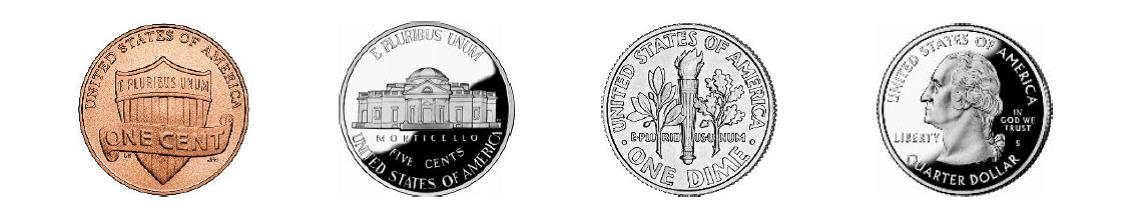
\includegraphics[width=0.9\textwidth]{coins.jpg}
\end{figure}
We consider the optimization problem whereby the change should be made
with the minimum number of coins possible.\\[5pt]
For example, if 27 cents change is to be made, this can be accomplished
with three coins (a quarter and two pennies) 27 pennies or various other
numbers of coins.
\end{EXAMPLE}
\end{spacing}
\end{frame}
\begin{frame}[t,allowdisplaybreaks,allowframebreaks]{Greedy Change-Making}
\begin{spacing}{1}
If $n$ is the amount of change required, we take the largest denomination
smaller than $n$, then consider the remaining amount. We again take the
largest denomination smaller than this amount and consider the
remainder, continuing until the original amount has been realized.\\[4pt]
\stepcounter{zhuo}
\alert{2.1.14. Algorithm.} \emph{(Greedy Change-making)}\\
\IncMargin{1em}
\begin{algorithm}[H]
\SetKwInput{Kw}{Input}\SetKwInput{Kt}{Output}
\SetKwFor{For}{for}{do}{end~for}
\SetKwFor{While}{while}{do}{end~while}
\Kw{$c_1>c_2>\,...\,>c_r$, coin denominations and $n$ a positive integer}
\Kt{$M$ a multiset of the $c_i,1\leq i\leq r$, with sum of all its elements being $n$}
$M\leftarrow\emptyset$\;
\For{$i\leftarrow 1$ \KwTo $r$}{
\While{$n\geq c_i$}{
add a coin with value $c_i$ to $M$\;
$n\leftarrow n-c_i$\;}}
\Return{$M$}
\end{algorithm}\DecMargin{1em}
\newpage
\vspace*{7pt}
Algorithm 2.1.14 is greedy, since at each step it takes the greatest
allowable denomination and adds it to the change. However, it is not
necessarily optimal, depending on the denominations available.\\[5pt]
For example, if only pennies, dimes and quarters are available (no nickels)
then change for 30 cents is made with one quarter and 5 pennies (6 coins)
while it would be optimal to make change using 3 dimes.\\[5pt]
It is thus not clear at all that the change-making algorithm is optimal
assuming available denominations of pennies, nickels, dimes and quarters.
As an illustration of the proof of optimality for algorithms, we will now
show that this is in fact the case. We first need a preliminary result.
\newpage
\vspace*{9pt}
\begin{LEMMA}
If $n$ is a positive integer, then $n$ cents in change using
quarters, dimes, nickels and pennies using the fewest coins possible has at
most two dimes, at most one nickel, at most four pennies and cannot have
two dimes and a nickel. The amount of change in dimes, nickels and
pennies cannot exceed 24 cents.\\[8pt]
\end{LEMMA}
\begin{PROOF}
The proof is a simple argument by contradiction. For example, if the
optimal solution had more than two dimes, we could replace them by a
quarter and a nickel, yielding a contradiction. The details are left to the reader.
\end{PROOF}
\vspace*{9pt}
\begin{THEOREM}
Given coin denominations of pennies, nickels, dimes and
quarters, Algorithm 2.1.14 produces change using the fewest coins
possible.
\end{THEOREM}
\newpage
\vspace*{7pt}
\begin{PROOF}
Suppose that there exists a number $n$ so that there is a way to make
change for $n$ using fewer coins than the greedy algorithm produces. First
we note that if $q'$ is the number of quarters in this optimal way and $q$ is
the number of quarters in the greedy algorithm, then $q = q'$. This follows,
because the greedy algorithm uses the most quarters possible $(q\geq q')$ and by Lemma 2.1.15 $q'\nless q$ (otherwise there would be $\geq25$ cents in dimes, nickels and pennies).\\[6pt]
Now both ways of making change must contain the same value of pennies,
nickels and dimes, since they contain the same number of quarters. There
must be the same number of dimes, since the greedy algorithm uses the
greatest number of dimes and in an optimal algorithm there are at most
one nickel and four pennies. Similarly, we also have the same number of
nickels and then also of pennies.
\end{PROOF}
\end{spacing}
\end{frame}
\begin{frame}[t]{Computational Complexity}
\begin{spacing}{1.1}
Implementing an algorithm generally requires resources, both of a physical
and a temporal type. That is, if we want to run an algorithm such as
Algorithm 2.1.3 for finding the maximum element of a set, we will need
computer hardware, in particular memory, as well as the time to run the
algorithm. Different algorithms may have different requirements; one
algorithm may require less time but more hardware resources than another.\\[5pt]
These requirements can be compared by considering the \emph{space complexity}
and the \emph{time complexity} of a given algorithm. The memory requirements
(space complexity) depend on the data structures used. We will not cover
this aspect of computer science in our course, and instead restrict our
analysis to the time complexity of algorithms.\\[5pt]
Time complexity is generally analyzed by considering the number of
operations an algorithm requires for completion instead of actual time.
This allows a comparison independent of specific computer characteristics
(processor speeds, parallel vs. serial processing etc.)
\end{spacing}
\end{frame}
\begin{frame}[t]{Time Complexity}
\begin{spacing}{1.05}
\begin{EXAMPLE}
Consider the time complexity of Algorithm 2.1.3 for finding the maximum element of a set. At each step, two comparisons are made:
\begin{itemize}
  \item one comparison to determine whether the end of the list has been reached and
  \item one comparison of the temporary maximum with the current element.
\end{itemize}
If the list has $n$ elements, these comparisons are performed $n-1$ times,
with an additional comparison to exit the loop. Therefore, a total of
$2n-1$ comparisons are made.\\[6pt]
It is not essential how many computer operations are necessary to
implement a single ``comparison'' or how long each comparison takes.
What is important is that when the list size doubles, so does (essentially)
the number of comparisons and hence the time needed for the algorithm.
The factor 2 and the subtraction of 1 is not relevant in practice.
\end{EXAMPLE}
\end{spacing}
\end{frame}
\begin{frame}[c]{Integer Sequences}
We now attempt to express this more formally. We associate to every
input size $n\in\N$ a number of steps $a_n\in\N$ that the algorithm needs to
complete. Hence, we mostly need to study integer sequences, but formally
we consider sequences with values in the real numbers, if necessary.
\end{frame}
\begin{frame}[t,allowdisplaybreaks,allowframebreaks]{The Landau Symbol $O$}
\begin{spacing}{1.05}
The integer sequences we consider will all diverge to infinity, with only
very few exceptions. Hence, we are not interested in their limits (a typical
problem in calculus) but rather in their relative \emph{speed of growth}.\\[4pt]
\begin{DEFINITION}
Let $(a_n)$ and $(b_n)$ be sequences. Then we say that
\setcounter{equation}{0}
\begin{equation}\label{2.1.1}
a_n=O(b_n)\qquad\qquad\quad(\text{as}~n\to\infty)
\end{equation}
(read as ``$(a_n)$ is big-oh of $(b_n)$'') if there exist constants $C\geq0$ and $N\in\N$ such that
\begin{equation}\label{2.1.2}
|a_n|\leq C|b_n|\qquad\qquad\quad\text{whenever}~n>N.
\end{equation}
\end{DEFINITION}
\stepcounter{zhuo}
\!\!\!\!\alert{2.1.19. Examples.}\\
\begin{itemize}
  \item[(i)] $n+n^2=O(n^2)$ as $n\to\infty$,
  \item[(ii)] $\displaystyle\sum_{k=1}^{n}\frac{1}{k}=O(\ln(n))$ as $n\to\infty$.
\end{itemize}
\newpage
\begin{REMARK}
The notation used in \eqref{2.1.1} is a little strange: $(a_n)$ is a sequence and hence $a_n$ is a number, but what is $O(b_n)$? It can not itself represent a number, because we have
\[n^2+1=O(n^2)\qquad\text{and}\qquad n^2+2=O(n^2)\qquad\text{but}\qquad
n^2+1\neq n^2+2.\]
So, clearly, the statement ``$n^2+1=O(n^2)$ as $n\to\infty$'' is a fixed expression and can only be understood in its entirety. The ``$=$'' symbol has a special meaning in this context.\\[5pt]
\end{REMARK}
\begin{REMARK}
From the definition of $O$ we see that ``$a_n=O(b_n)$ as $n\to\infty$'' means that the terms $a_n$ are bounded by a constant times $b_n$.\\[4pt]
We can think of this as meaning that the terms of $(a_n)$ are ``not much larger'' than those of $(b_n)$.
\end{REMARK}
\newpage
\begin{REMARK}
It is not actually necessary in \eqref{2.1.2} to require the existence of an $N>0$ such that the inequality holds for $n>N$; since there are only finitely many terms $a_0,a_1\,...\,,a_{N-1}$ before $N$, there exists a constant $C$ such that \eqref{2.1.2}  holds for $n>N$ if and only if that is the case for all $n\in\N$. However, we have left the definition as it stands because it
is then closer to the analogous definition for functions.\\[5pt]
In most cases, it is not necessary to check the definition when comparing $(a_n)$ with $(b_n)$, as the following useful result holds:\\[5pt]
\begin{THEOREM}
Let $(a_n)$ and $(b_n)$ be sequences. If there exists some $C\geq0$ such that
\[\lim_{n\to\infty}\frac{|a_n|}{|b_n|}=C,\]
then $a_n=O(b_n)$ as $n\to\infty$.
\end{THEOREM}
\end{REMARK}
\end{spacing}
\end{frame}
\begin{frame}[t]{Landau Symbols using Limits}
\begin{spacing}{1}
\begin{PROOF}
Assume that for some $C\geq0$
\[\lim_{n\to\infty}\frac{|a_n|}{|b_n|}=C.\]
Then
\[\mathop{\forall}_{m\in\N}\mathop{\exists}_{N>0}\mathop{\forall}_{n\in\N}
\:n>N\Rightarrow\left|\frac{|a_n|}{|b_n|}-C\right|<\frac{1}{m}.\]
Choose $m=1$. Then there exists some $N>0$ such that $n>N$ implies
\[\big||a_n|-C|b_n|\big|<|b_n|,\]
i.e.,
\[|a_n|\leq(C+1)|b_n|.\]
This is just the definition of $a_n=O(b_n)$ as $n\to\infty$.
\end{PROOF}
\end{spacing}
\end{frame}
\begin{frame}[t]{Variants of Landau Symbols}
\begin{spacing}{1.05}
If $a_n=O(b_n)$, then the values of $a_n$ are not larger than a constant (independent of $n$) times the values of $b_n$ when $n$ is large enough. However, $a_n$ can actually be much smaller than $b_n$, e.g., we could write
\[\frac{1}{n}=O(n^{100})\]
which would be correct, but pretty meaningless. In many practical
applications, one wants to express that not only is $a_n$ not much larger than
$b_n$, but also it is not much smaller. Physicists have often done this by
defining special variants of Landau symbols, which look identical but
according to the publication in which they occur are defined differently.
This can of course lead to some confusion.\\[5pt]
To clarify the situation, the computer scientist Donald E. Knuth has
introduced common variants using different symbols. To my knowledge,
they are, however, not widely used in the physics and mathematics
literature.
\end{spacing}
\end{frame}
\begin{frame}[c]{The $\Omega$ and $\Theta$ Symbols}
\begin{spacing}{1.1}
The symbol $O$ in the expression $a_n=O(b_n)$ essentially gives an upper growth bound for $a_n$. The following symbols also give lower growth bounds:\\[5pt]
\begin{DEFINITION}
Let $(a_n)$ and $(b_n)$ be sequences. Then we define, as $n\to\infty$,
\begin{equation}\label{2.1.3}
a_n=\Omega(b_n)\qquad\qquad\qquad:\Leftrightarrow
\qquad\qquad\qquad b_n=O(a_n),
\end{equation}
read ``$(a_n)$ is big-omega of $(b_n)$''.\\[4pt]
Furthermore, we define
\begin{equation}\label{2.1.4}
a_n=\Theta(b_n)\qquad\qquad:\Leftrightarrow\qquad
\qquad a_n=O(b_n)~and~a_n=\Omega(b_n),
\end{equation}
read ``$(a_n)$ is big-theta of $(b_n)$''.
\end{DEFINITION}
\end{spacing}
\end{frame}
\begin{frame}[t,allowdisplaybreaks,allowframebreaks]{Time Complexity of Bubble Sort}
\begin{spacing}{1}
\vspace*{-6pt}
\begin{EXAMPLE}
Consider the time complexity of Algorithm 2.1.11 (Bubble Sort). During the $i$th pass, $n-i$ comparisons are used and $n-1$ passes are made. The total number of comparisons is then
\[\sum_{i=1}^{n-1}(n-i)=n(n-1)-\frac{n(n-1)}{2}=
\frac{n(n-1)}{2}\]
Since
\[\frac{1}{4}n^2\leq\frac{n(n-1)}{2}\leq\frac{1}{2}n^2
\qquad\qquad\quad\text{for}~n\geq2\]
we see that
\[\sum_{i=1}^{n-1}(n-i)=\Theta(n^2)\]
\end{EXAMPLE}
This tells us that the number of comparisons of list elements grows
quadratically with the size of the list. That means that if the list size is
doubled, the number of list element comparisons required to sort the list
grows fourfold.
\newpage
We should also take into account that comparisons are made in each of
the loops to detect whether the loop indices $i$ and $j$ have reached their
limit. In fact, there is one such comparison for each comparison of list
elements (since at each step of the algorithm, there is one list element
comparison) and we hence have
\[\sum_{i=1}^{n-1}(n-i)=\Theta(n^2)\]
comparisons to see if the loops have terminated.\\[5pt]
From this we see that there are a total of
\[\Theta(n^2)+\Theta(n^2)=\Theta(n^2)\]
comparisons. Hence, the comparisons of the loop variables do not affect
the time complexity of the Bubble Sort algorithm.
\end{spacing}
\end{frame}
\begin{frame}[t,allowdisplaybreaks,allowframebreaks]{Interpreting the Time Complexity of Algorithms}
\begin{spacing}{1.05}
\begin{REMARK}
In nearly all practical applications, the number of
comparisons used to see if a loop has ended is not larger than the number
of comparisons (or operations) used within a loop. Therefore, in most
cases, it is fine to neglect these comparisons when determining the
complexity of an algorithm.\\[5pt]
It is also important to define precisely in what terms complexity is
expressed and what it measures; in Example 2.1.25, the complexity
measures
\begin{quote}
  the number of comparisons as a function of list length.
\end{quote}
However, in practice, comparing two large numbers with many digits takes
more time than comparing two small numbers. This is not taken into
account in our analysis. This is not a problem, but we need to state clearly
at all times, what we are expressing by a given complexity.
\newpage
Also, in Example 2.1.25, the shifts that are performed (where an element
is moved to another position in the list) are not counted. It is assumed
that the ``cost'' of these shifts (the time needed to perform them) is small
compared to the time needed for comparisons.\\[5pt]
All this should make clear that the (asymptotic) time complexities we are
calculating do not completely reflect the practical speed at which different
algorithms can run. The asymptotic time complexity expresses the
behavior of an algorithm at infinity, that is in the limit of infinite input
size. In practice, an algorithm with a worse asymptotic complexity could
perform better than another one with a lower complexity, since in practice
the input size is finite.\\[5pt]
For example, both Insertion Sort and Bubble Sort need $O(n^2)$
comparisons, but their actual speed may be different when both are
implemented on the same computer.
\end{REMARK}
\end{spacing}
\end{frame}
\begin{frame}[c]{Categorization of Complexities}
\begin{spacing}{1.15}
In general, we distinguish between the following complexities for
algorithms (in increasing order of complexity):
\begin{center}
  \begin{tabular}{ll}
  \toprule
    Complexity & Terminology \\ \midrule
    $\Theta(1)$ & constant complexity \\
    $\Theta(\log n)$ & logarithmic complexity \\
    $\Theta(n)$ & linear complexity \\
    $\Theta(n\log n)$ & $n\log n$ complexity \\
    $\Theta(n^b),~b>0$ & polynomial complexity \\
    $\Theta(b^{n^\varepsilon}),\:b>1,\,0<\varepsilon<1$ & sub-exponential complexity \\
    $\Theta(b^n),~b>1$ & exponential complexity \\
    $\Theta(n!)$ & factorial complexity \\
  \bottomrule
  \end{tabular}
\end{center}
\end{spacing}
\end{frame}
\begin{frame}[t,allowdisplaybreaks,allowframebreaks,fragile]{Merge Sort}
\begin{spacing}{1.05}
\begin{columns}[onlytextwidth]
\begin{column}{0.3\textwidth}
An efficient sorting algorithm
that can be
formulated recursively
is the \emph{merge sort}.
It works by successively
splitting a list
in half until only lists
of length 1 remain.
These are then successively
joined to ordered
lists.\\[5pt]
We illustrate by showing
how merge sort orders
the list $8, 2, 4,
6, 9, 7, 10, 1, 5, 3$ at
right.
\end{column}
\begin{column}{0.7\textwidth}
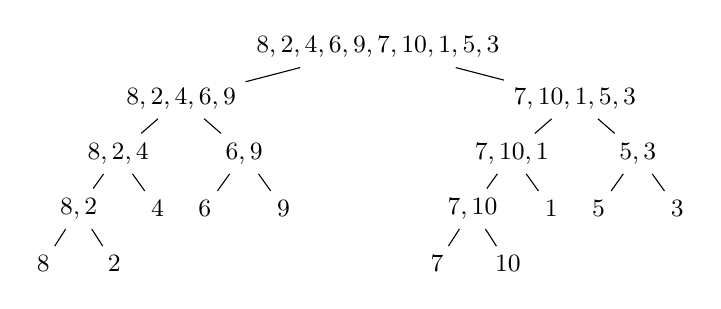
\begin{tikzpicture}
[font=\small,
      level 1/.style={sibling distance=5cm,level distance=0.65cm},
      level 2/.style={sibling
      distance=1.6cm,level distance=0.7cm},
      level 3/.style={sibling distance=1cm,level distance=0.7cm},
      level 4/.style={sibling
      distance=0.9cm,level distance=0.7cm}]
 \node {$8,2,4,6,9,7,10,1,5,3$}
  child { node {$8,2,4,6,9$}
   child { node {$8,2,4$}
    child { node {$8,2$}
     child { node {$8$}}
     child { node {$2$}}}
    child { node {$4$}}}
   child { node {$6,9$}
    child { node {$6$}}
    child { node {$9$}}}}
  child { node {$7,10,1,5,3$}
   child { node {$7,10,1$}
    child { node {$7,10$}
     child { node {$7$}}
     child { node {$10$}}}
    child { node {$1$}}}
   child { node {$5,3$}
    child { node {$5$}}
    child { node {$3$}}}};
\end{tikzpicture}
\rule[5pt]{\columnwidth}{1pt}
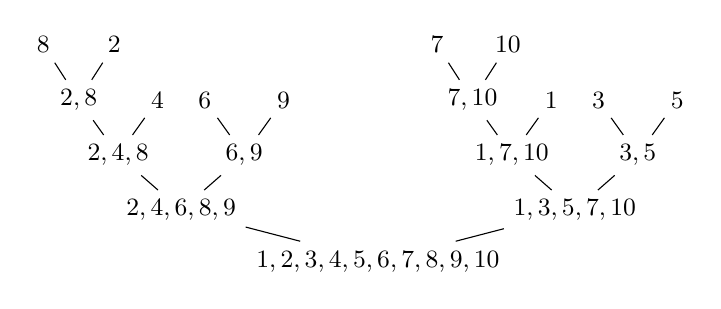
\begin{tikzpicture}
[font=\small,grow=north,
      level 1/.style={sibling distance=5cm,level distance=0.65cm},
      level 2/.style={sibling
      distance=1.6cm,level distance=0.7cm},
      level 3/.style={sibling distance=1cm,level distance=0.7cm},
      level 4/.style={sibling
      distance=0.9cm,level distance=0.7cm}]
 \node {$1,2,3,4,5,6,7,8,9,10$}
  child { node {$1,3,5,7,10$}
  child { node {$3,5$}
    child { node {$5$}}
    child { node {$3$}}}
   child { node {$1,7,10$}
   child { node {$1$}}
    child { node {$7,10$}
     child { node {$10$}}
     child { node {$7$}}}
    }
   }
  child { node {$2,4,6,8,9$}
  child { node {$6,9$}
    child { node {$9$}}
    child { node {$6$}}}
   child { node {$2,4,8$}
   child { node {$4$}}
    child { node {$2,8$}
     child { node {$2$}}
     child { node {$8$}}}
    }};
\end{tikzpicture}
\end{column}
\end{columns}
\newpage
The recursive pseudocode for merge sort is quite simple; it depends on
having an algorithm for merging two ordered lists into a single ordered list:\\[5pt]
\stepcounter{zhuo}
\alert{2.1.27. Algorithm.} \emph{(Merge Sort)}
\IncMargin{1em}
\begin{algorithm}[H]
\SetKwInput{Kw}{Input}\SetKwInput{Kt}{Output}
\SetKwFunction{Merge}{MergeSort}
\SetKwFunction{Mer}{Merge}
\SetKwIF{If}{ElseIf}{Else}{if}{then}{else if}{else}{end~if}
\SetKwBlock{Function}{Function \Merge{$L$}:}{end}
\Kw{$L=a_1\,,...\,,a_n$}
\Kt{$L$, sorted into elements in nondecreasing order}
\Function{\If{$n>1$}{
$m\leftarrow\lfloor n/2\rfloor$\;
$L_1\leftarrow a_1,\,...\,,a_m$\;
$L_2\leftarrow a_{m+1},\,...\,,a_n$\;
$L\leftarrow$\Mer{\Merge{$L_1$},\Merge{$L_2$}}}
\Return $L$}
\end{algorithm}\DecMargin{1em}
\end{spacing}
\end{frame}
\begin{frame}[t]{Merging Two Sorted Lists}
\begin{spacing}{1}
\stepcounter{zhuo}
\alert{2.1.28. Algorithm.} \emph{(Merge)}
\IncMargin{1em}
\begin{algorithm}[H]
\SetKwInput{Kw}{Input}\SetKwInput{Kt}{Output}
\SetKwFunction{Mer}{Merge}
\SetKwIF{If}{ElseIf}{Else}{if}{then}{else if}{else}{end~if}
\SetKwFor{While}{while}{do}{end~while}
\SetKwBlock{Function}{Function \Merge{$L_1,L_2$}:}{end}
\Kw{$L_1,L_2$, two sorted lists}
\Kt{$L$ a merged list of $L_1$ and $L_2$, with elements in increasing order}
\Function{\ShowLn$L\leftarrow$ empty list\;
\While{$L_1~and~L_2~are~both~nonempty$}{
 remove smaller of first element of $L_1$ and $L_2$ from the list it is in and put it at the right end of $L$\;
\If{\emph{removal of this element makes one list empty}}{
 remove all elements from the other list and append to $L$}}
\Return $L$}
\end{algorithm}\DecMargin{1em}
\end{spacing}
\end{frame}
\begin{frame}[t]{Complexity of Merging Two Sorted Lists}
\begin{spacing}{1.1}
\begin{LEMMA}
Two sorted lists with $m$ and $n$ elements, respectively, can be merged into a sorted list using no more than $n+m-1$ comparisons.\\[6pt]
\end{LEMMA}
\begin{PROOF}
The least efficient way for Algorithm 2.1.28 to run is for none of the lists to become empty while the other has more than one element in it. Then $m-1+n-1$ comparisons are made, The final comparison is then made between the remaining two elements.
\end{PROOF}
\end{spacing}
\end{frame}
\begin{frame}[t,allowdisplaybreaks,allowframebreaks]{Complexity of Merge Sort}
\begin{spacing}{1.1}
We now analyze the efficiency of merge sort. Recall that bubble sort needed $\Theta(n^2)$ comparisons to sort a list with $n$ elements. Merge sort is rather more efficient.\\[6pt]
\begin{THEOREM}
The number of comparisons needed to merge sort a list with $n$ elements is $O(n\log n)$.\\[6pt]
\end{THEOREM}
\begin{PROOF}
We assume that $n=2^m$ for simplicity. If this is not the case, the following
arguments can be modified and will yield the same result.\\[5pt]
At the first stage of the splitting procedure, the list is split into two
sublists with $2^{m-1}$ elements each. This procedure is repeated, and after $k$ splittings, there are $2^k$ sublists with $2^{m-k}$ elements each. After $m$ steps, there are $2^m$ lists of length 1. These $2^m$ lists are merged into $2^{m-1}$ lists of length 2, requiring $2^{m-1}$ comparisons.
\newpage
\alert{Proof (continued).}\\
This procedure continues and generalizes as follows: at level $k$\\
$(k=m,m-1,\,...\,,2,1)~2^k$ lists each with $2^{m-k}$ elements are merged into $2^{k-1}$ lists. By Lemma 2.1.29, each of the $2^{k-1}$ mergers requires at most $2^{m-k}+2^{m-k}-1=2^{m-k+1}-1$ comparisons.\\[6pt]
The total number of comparisons is required is then
\begin{equation*}
  \begin{split}
     \sum_{k=1}^{m}2^{k-1}(2^{m-k+1}-1) &=\sum_{k=1}^{m}2^m-\sum_{k=1}^{m}2^{k-1} \\
       &=m2^m-(2^m-1) \\
       &=n\log n-n+1.
  \end{split}
\end{equation*}
\end{PROOF}
\end{spacing}
\end{frame}
\begin{frame}[c]{Efficiency of Sorting}
\begin{spacing}{1.2}
The merge sort algorithm is ``optimal'' in the following sense:\\[5pt]
\begin{THEOREM}
A sorting algorithm based on comparisons of pairs of elements needs $\Omega(n\log n)$ comparisons to sort a list of $n$ elements.\\[5pt]
We will prove this theorem later in the context of the theory of trees.\\[5pt]
In the following section, we consider several computational algorithms
arising in number theory and cryptography.
\end{THEOREM}
\end{spacing}
\end{frame}
\subsection{Computer Arithmetic}
\begin{frame}[c] \begin{spacing}{2.5}
\tableofcontents[sectionstyle=hide,subsectionstyle=show/shaded/hide] \end{spacing}
\end{frame}
\begin{frame}[t,allowdisplaybreaks,allowframebreaks]{Representations of Integers}
\begin{spacing}{1.0}
In the first part of the course, the properties of numbers in general and
integers in particular were investigated. The results we obtained are
generally applicable to integers, without regard to the way in which they
are represented.\\[5pt]
However, to implement these theorems and methods in practice, a
concrete representation of integers needs to be chosen. Moreover,
choosing a beneficial representation may allow algorithms to be run more
efficiently than in certain other representations.\\[5pt]
It is common to represent numbers in terms of decimal notation, e.g., we
write
\[124=1\cdot10^2+2\cdot10^1+4\cdot10^0.\]
However, nothing is special about the number 10 and we could also write
\[124=1\cdot8^2+7\cdot8^1+4\cdot8^0\]
using the \emph{base} 8.
\newpage
\stepcounter{zhuo}
\alert{2.2.1. Definition and Theorem.} Let $b\in\N\setminus\{0,1\}$ and $a\in\N\setminus\{0\}$. Then there exist unique numbers $a_0,\,...\,,a_k<b$ with $a_k\neq0$ such that
\setcounter{equation}{0}
\begin{equation}\label{2.2.1}
a=a_kb^k+a_{k-1}b^{k-1}+\cdots+a_1b+a_0.
\end{equation}
The representation \eqref{2.2.1} is called the \emph{base b expansion of a}. The numbers $a_k$ are called the \emph{digits} of $a$ in base $b$.\\[5pt]
The proof of Theorem 2.2.1 can be performed using induction. We will omit it here.\\[5pt]
Several bases are in common use:
\begin{itemize}
  \item $b=2$ (binary)
  \item $b=8$ (octal)
  \item $b=10$ (decimal)
  \item $b=16$ (hexadecimal)
\end{itemize}
\end{spacing}
\newpage
\begin{spacing}{1.2}
Analogously to the case $b = 10$ we will give a number in a base $b$ simply
by listing its digits in this base. We indicate the base of the expansion by a
subscript as follows:
\[124=(124)_{10}=(174)_8.\]
For the hexadecimal expansion we represent the digits $a_j$ in \eqref{2.2.1} through
\[0,1,2,3,4,5,6,7,8,9,\sf{A,B,C,D,E,F}.\]
For example, the number $(2AE0B)_{16}$ is given by
\[2\cdot16^4+10\cdot16^3+14\cdot16^2+0\cdot16+11
=(175627)_{10}.\]
\end{spacing}
\end{frame}
\begin{frame}[t,allowdisplaybreaks,allowframebreaks]{Base Conversion}
\begin{spacing}{1.05}
The table below gives the numbers 0 through 15 in different base expansions.
\begin{center}
\begin{tabular}{ccccccccc}
\toprule
  Decimal & 0 & 1 & 2 & 3 & 4 & 5 & 6 & 7\\
  Hexadecimal & 0 & 1 & 2 & 3 & 4 & 5 & 6& 7 \\
  Octal & 0 & 1 & 2 & 3 & 4 & 5 & 6 & 7 \\
  Binary & 0 & 1 & 10 & 11 & 100 & 101 & 110 & 111 \\ \midrule
  Decimal & 8 & 9 & 10 & 11 & 12 & 13 & 14& 15 \\
  Hexadecimal & 8 & 9 & A & B & C & D & E& F \\
  Octal & 10 & 11 & 12 & 13 & 14 & 15 & 16& 17 \\
  Binary & 1000 & 1001 & 1010 & 1011 & 1100 & 1101 & 1110 & 1111 \\
  \bottomrule
\end{tabular}
\end{center}
It is very easy to convert between binary and hexadecimal expansions
because each hexadecimal digit corresponds to a block of four binary digits
(as listed above with leading zeroes omitted). For example,
\[(1101~1001~1100~0000)_2=(\sf{D9C0})_{16}.\]
\newpage
To represent a given number $a$ in an arbitrary base $b$ we proceed as follows:
\[a=a_kb^k+a_{k-1}b^{k-1}+\cdots+a_1b+a_0\]
so by the Division Algorithm 1.6.1 we obtain
\[a_0=a\:\text{mod}\:b.\]
Let
\[q_0=a\:\text{div}\:b=\frac{a-a_0}{b}.\]
Then
\[a_1=q_0\:\text{mod}\:b\qquad\qquad
\text{and we set}\qquad\qquad
q_1=q_0\:\text{div}\:b.\]
Continuing this process until $q_k\:\text{div}\:b=0$ for some $k\in\N$, we find all coefficients of the base $b$ expansion.
\newpage
\vspace*{9pt}
\begin{EXAMPLE}
To find the octal expansion of $(12345)_{10}$ we first divide by 8 to obtain $12345=8\cdot1543+1$, so\\[6pt]
\begin{center}
\begin{tabular}{cl}
  $1543=12345~\text{div}~8,$ & $1=12345~\text{mod}~8$, \\[3pt]
  $192=1543~\text{div}~8,$ & $7=1543~\text{mod}~8$, \\[3pt]
  $24=192~\text{div}~8,$ & $0=192~\text{mod}~8$, \\[3pt]
  $3=24~\text{div}~8,$ & $0=24~\text{mod}~8$, \\[3pt]
  \!\!$0=3~\text{div}~8,$ & $3=3~\text{mod}~8$. \\[3pt]
\end{tabular}
\end{center}
We hence obtain $(12345)_{10}=(30071)_8$.
\end{EXAMPLE}
\end{spacing}
\end{frame}
\begin{frame}[t]{Pseudocode for Base Conversion}
\begin{spacing}{1.05}
\stepcounter{zhuo}
\alert{2.2.3. Algorithm.} \emph{(Base Expansion)}
\IncMargin{1em}
\begin{algorithm}[H]
\SetKwInput{Kw}{Input}\SetKwInput{Kt}{Output}
\SetKwFor{While}{while}{do}{end~while}
\Kw{$a$, a positive integer}
\Kt{$A=(a_n\ldots a_0)_b$, the expansion of $a$ in base $b$}
$q\leftarrow a$;~$k\leftarrow0$;~$A\leftarrow()_b$\;
\While{$q\neq0$}{
$a_k\leftarrow q~\text{mod}~b$\;
prepend $a_k$ to $A$\;
$q\leftarrow q~\text{div}~b$\;
$k\leftarrow k+1$\;}
\Return A
\end{algorithm}\DecMargin{1em}
\vspace*{6pt}
The number of operations used by the algorithm depends on the
implementation of the Division Algorithm used to calculate $q$ mod $b$ and $q$ div $b$.
\end{spacing}
\end{frame}
\begin{frame}[c]{Computer Arithmetic}
\begin{spacing}{1.1}
Computers work with numbers in binary representation (also called \emph{binary
numbers} for short), e.g.,
\[(1000)_{10}=(1111101000)_2\]
The sequence of numbers on the right-hand side, 1111101000, is called a \emph{bit string} and each digit is called a \emph{bit}.\\[5pt]
A bit string of length 8 (called a \emph{byte}) stores a number of size between 0 and $2^8-1$. One byte can also be represented by two hexadecimal digits.\\[6pt]
We will now consider several algorithms for basic arithmetic operations,
starting with addition. These operations will assume that numbers are
given in binary representation.
\end{spacing}
\end{frame}
\begin{frame}[t]{Addition of Integers}
\begin{spacing}{1}
Let $a=(a_{n-1}a_{n-2}\,...\,a_0)_2$ and $b=(b_{n-1}b_{n-2}\,...\,b_0)_2$ be two binary numbers. We then calculate their sum
\[s=a+b=(s_ns_{n-1}s_{n-2}\,...\,s_0)_2\]
as follows: We start with adding the right-most digits,
\begin{equation}\label{2.2.2}
a_0+b_0=c_0\cdot2+s_0
\end{equation}
so that $s_0$ is the right-most digit of $a+b$ and $c_0$ is called the \emph{carry}.\\[6pt]
We next add
\[a_1+b_1+c_0=c_1\cdot2+s_1,\]
so that $(a+b)_1=s_1$. We continue this procedure until we reach
\[a_{n-1}+b_{n-1}+c_{n-2}=c_{n-1}\cdot2+s_{n-1}.\]
Finally, $s_n=c_{n-1}$ is the leading digit of $s$.
\end{spacing}
\end{frame}
\begin{frame}[t]{Pseudocode for the Addition of Integers}
\begin{spacing}{1.05}
\stepcounter{zhuo}
\alert{2.2.4. Algorithm.} \emph{(Integer Addition in Base 2)}
\IncMargin{1em}
\begin{algorithm}[H]
\SetKwInput{Kw}{Input}\SetKwInput{Kt}{Output}
\SetKwFor{For}{for}{do}{end~for}
\Kw{$a=(a_{n-1}a_{n-2}\,...\,a_0)_2$ and $b=(b_{n-1}b_{n-2}\,...\,b_0)_2$}
\Kt{$s=(s_n\,...\,s_0)_2=a+b$}
$c\leftarrow0\,;\,s\leftarrow()_2$\;
\For{$j\leftarrow0$ \KwTo $n-1$}{
\lIf{$a_j+b_j+c_j\leq1$}{$d=0$}~\lElse{$d=1$}\;
$s_j\leftarrow a_j+b_j+c-2d$\;
prepend $s_j$ to $s$\;
$c\leftarrow d$\;}
append $c$ to $s$\;
\Return s
\end{algorithm}\DecMargin{1em}
\vspace*{5pt}
\begin{REMARK}
A similar algorithm for subtraction will be part of the assignments.
\end{REMARK}
\end{spacing}
\end{frame}
\begin{frame}[c]{Complexity of Addition of Integers}
\begin{spacing}{1.1}
\begin{REMARK}
The addition of two bits as in \eqref{2.2.2} is a single \emph{bit
operation} and we will express the complexity of algorithms in terms of
such bit operations. (This is similar to our discussion of sorting algorithms,
where the complexity was expressed in terms of elementary \emph{comparisons}.)\\[5pt]
It is easy to see that if $a$ and $b$ are $n$-digit binary numbers, Algorithm 2.2.4 uses
\[O(n)=O(\log_2(a))=O(\log_{10}(a))\]
additions of bits.\\[8pt]
Multiplication also works in the same way as it is taught in school.
However, since the numbers are in binary representation, there is a small
advantage: instead of bit-wise multiplications, only bit-wise shifts need to
be performed.
\end{REMARK}
\end{spacing}
\end{frame}
\begin{frame}[c]{Pseudocode for the Multiplication of Integers}
\begin{spacing}{1.05}
\stepcounter{zhuo}
\alert{2.2.7. Algorithm.} \emph{(Integer Multiplication in Base 2)}
\IncMargin{1em}
\begin{algorithm}[H]
\SetKwInput{Kw}{Input}\SetKwInput{Kt}{Output}
\SetKwFor{For}{for}{do}{end~for}
\Kw{$a=(a_{n-1}a_{n-2}\,...\,a_0)_2$ and $b=(b_{n-1}b_{n-2}\,...\,b_0)_2$}
\Kt{$p=a\cdot b$}
\For(\tcc*[f]{$c_0,\,...\,,c_{n-1}$: partial products}){$j\leftarrow0$ \KwTo $n-1$}{
\lIf{$b_j=1$}{$c_j=a$ shifted $j$ places}\;
\lElse{$c_j=0$}\;}
$p_0\leftarrow1$\;
\For{$j\leftarrow0$ \KwTo $n-1$}{
$p\leftarrow p+c_j$}
\Return p
\end{algorithm}\DecMargin{1em}
\end{spacing}
\end{frame}
\begin{frame}[c]{Complexity of Integer Multiplication}
\begin{spacing}{1.1}
For each partial product $c_j$, $n$ bits need to be shifted. Since there are $n$ partial products, this means that $O(n^2)$ bit shift operations are necessary. Finally, $n$ numbers need to be added, each addition requiring $O(n)$ bit additions. We hence have in total
\[O(n^2)+n\cdot O(n)=O(n^2)\]
bit operations.\\[7pt]
\begin{REMARK}
There exist more efficient algorithms for multiplication. One, which we will introduce later in Example 2.3.6, uses $O(n^{\log3})=O(n^{1.584})$ operations.\\[5pt]
Let us now consider the division algorithm, which is also the foundation of
the base conversion Algorithm 2.2.3.
\end{REMARK}
\end{spacing}
\end{frame}
\begin{frame}[t]{Pseudocode for the Division Algorithm}
\begin{spacing}{1.1}
\stepcounter{zhuo}
\alert{2.2.9. Algorithm.} \emph{(The Division Algorithm - \sf div \emph{and} mod\emph{)}}
\IncMargin{1em}
\begin{algorithm}[H]
\SetKwInput{Kw}{Input}\SetKwInput{Kt}{Output}
\SetKwFor{While}{while}{do}{end~while}
\SetKwIF{If}{ElseIf}{Else}{if}{then}{else if}{else}{end~if}
\Kw{$a$ an integer and $d$ a positive integer}
\Kt{$q=a~\text{div}~d$ and $r=a~\text{mod}~d$}
$q\leftarrow0;r\leftarrow|a|$\;
\While{$r\geq d$}{
$r\leftarrow r-d$\;
$q\leftarrow q+1$\;}
\If{$a<0~and~r>0$}{
$r\leftarrow d-r$\;
$q\leftarrow -(q+1)$\;}
\Return $q,r$
\end{algorithm}\DecMargin{1em}
\end{spacing}
\end{frame}
\begin{frame}[c]{Efficiency of the Division Algorithm}
Algorithm 2.2.9 uses $O(q\log a)$ bit operations.\\
\begin{REMARK}
There exist more efficient algorithms that require only $O(\log a\cdot\log d)$ operations.
\end{REMARK}
\end{frame}
\begin{frame}[t,allowdisplaybreaks,allowframebreaks]{Computer Arithmetic with Large Integers}
\begin{spacing}{1}
The previously discussed operations for addition and multiplication do not
scale very well when very large numbers (with thousands of digits or more)
are to be manipulated. The following approach is a way around this.\\[5pt]
Let $m_1,\,...\,,m_n\in\N\setminus\{0,1\}$ be pairwise relatively prime, $m=\prod_{i=1}^{n}m_i$ and $a\in\Z$ with $0\leq a<m$. Then it follows from the Chinese Remainder
Theorem (see exercises) that $a$ is uniquely determined by the $n$-tuple
\[(a~\text{mod}~m_1,\,...\,,a~\text{mod}~m_n).\]
\begin{EXAMPLE}
Take $m_1=3,\,m_2=4$. Then all integers less than $3\cdot4=12$ can be represented using their remainders upon division by 3
and 4 as follows:
\begin{center}
 \begin{tabular}{ccccccc}
   \toprule
   $n$ & 0 & 1 & 2 & 3 & 4 & 5 \\
   $(n~\text{mod}~3,\,n~\text{mod}~4)$ & $(0,0)$ & $(1,1)$ & $(2,2)$ & $(0,3)$ & $(1,0)$ & $(2,1)$ \\ \midrule
   $n$ & 6 & 7 & 8 & 9 & 10 & 11 \\
   $(n~\text{mod}~3,\,n~\text{mod}~4)$ & $(0,2)$ & $(1,3)$ & $(2,0)$ & $(0,1)$ & $(1,2)$ & $(2,3)$ \\
   \bottomrule
 \end{tabular}
\end{center}
\end{EXAMPLE}
\end{spacing}
\newpage
\begin{spacing}{0.9}
We can now perform arithmetic operations on these tuples of integers
instead of the original number.\\[5pt]
\begin{EXAMPLE}
The numbers $95,97,98,99$ are pairwise relatively prime. Then we can represent any integer less than $99\cdot98\cdot97\cdot95=89\,403\,930$ as a quadruple of the remainders with respect to these numbers.\\[5pt]
To calculate the sum $123684+413456$ we first represent the summands as quadruples $(n~\text{mod}~99,\,n~\text{mod}~98,\,n~\text{mod}~97,\,
n~\text{mod}~95)$ and then add them:
\begin{equation*}
  \begin{split}
       &~~~~(33,8,9,89)+(32,92,42,16) \\
       &=(65\,\text{mod}\,99,\,100\,\text{mod}\,98,\,
       51\,\text{mod}\,97,\,105\,\text{mod}\,95)  \\
       &=(65,2,51,10)
  \end{split}
\end{equation*}
To convert the result back to a number, we solve the system of congruences
\[x\equiv65\:(\text{mod}\,99),~~x\equiv2\:(\text{mod}\,98),~~
x\equiv52\:(\text{mod}\,97),~~x\equiv10\:(\text{mod}\,95)\]
and find $x=537\,140$.
\end{EXAMPLE}
\end{spacing}
\end{frame}
\begin{frame}[c]{Modular Exponentiation}
\begin{spacing}{1.1}
In cryptography, for example in the Diffie-Hellman Key Agreement Protocol, it is necessary to calculate $b^n\,\text{mod}\,m$ efficiently, where $n\in\N,b\in\Z$ and $m\in\N\setminus\{0,1\}$. In general, $b^n$ will be very large, so it is not practical to calculate $b^n$ first and then compute the modulus.\\[6pt]
We first develop an efficient strategy for exponentiation (more efficient
than multiplying as in Algorithm 2.2.7) and combine it with finding the
remainder. We use the binary expansion of $n$ to compute $b^n$:
\[b^n=b^{a_{k-1}2^{k-1}+\cdots+a_1\cdot2+a_0}=\prod_{j=0}^{k-1}
b^{a_j2^j},\qquad\qquad a_0,\,...\,,a_{k-1}\in\{0,1\}.\]
We first find all powers $b^{2^j}$ recursively, by noting that $b^{2^{j+1}}=(b^{2^j})^2$. Next we calculate their values mod $m$ and finally compute their product.
\end{spacing}
\end{frame}
\begin{frame}[c]{Pseudocode for Modular Exponentiation}
\begin{spacing}{1.1}
\stepcounter{zhuo}
\alert{2.2.13. Algorithm.} \emph{(Modular Exponentiation)}\\[2pt]
\IncMargin{1em}
\begin{algorithm}[H]
\SetKwInput{Kw}{Input}\SetKwInput{Kt}{Output}
\SetKwFor{For}{for}{do}{end~for}
\Kw{$b$ an integer, $n=(n_{k-1}\,...\,n_0)_2$ and $m$ two positive integers}
\Kt{$x=b^n\mod m$}
$x\leftarrow1;\,power\leftarrow b\,\text{mod}\:m$\;
\For{$i\leftarrow0$ \KwTo $k-1$}{
\lIf{$n_i=1$}{$x\leftarrow(x\cdot power)\,\text{mod}\,m$}\;
$power\leftarrow(power\cdot power)\,\text{mod}\,m$\;}
\Return{$x$}
\end{algorithm}\DecMargin{1em}
\vspace*{7pt}
Supposing that the more efficient division algorithm referred to in Remark 2.2.10 is used, Algorithm 2.2.13 uses $O((\log m)^2\log n)$ bit operations to find $b^n\,\text{mod}\,m$.
\end{spacing}
\end{frame}
\begin{frame}[t]{Pseudocode for the Euclidean Algorithm}
\begin{spacing}{1.1}
We close this section with a discussion of the Euclidean algorithm:\\[5pt]
\stepcounter{zhuo}
\alert{2.2.14. Algorithm.} \emph{(The Euclidean Algorithm)}\\[2pt]
\IncMargin{1em}
\begin{algorithm}[H]
\SetKwInput{Kw}{Input}\SetKwInput{Kt}{Output}
\SetKwFor{While}{while}{do}{end~while}
\Kw{$a,b$, two positive integers}
\Kt{$x=\gcd(a,b)$}
$x\leftarrow a;y\leftarrow b$\;
\While{$y\neq0$}{
$r\leftarrow x\,\text{mod}\,y$\;
$x\leftarrow y;y\leftarrow r$\;
}
\Return{$x$}
\end{algorithm}
\DecMargin{1em}
\vspace*{5pt}
The following theorem is noteworthy, because its proof uses an ``inverse''
approach to finding the complexity: instead of asking how many
operations are needed for a given input, it discusses the input size if a
given number of operations are used.
\end{spacing}
\end{frame}
\begin{frame}[t,allowdisplaybreaks,allowframebreaks]{Efficiency of the Euclidean Algorithm}
\begin{spacing}{1.05}
\stepcounter{zhuo}
\alert{2.2.15. Lam\'{e}'s Theorem.} Let $a,b\in\N\setminus\{0\}$ with $a\geq b$. Then the number of divisions used by the Euclidean Algorithm to find $\gcd(a,b)$ is not greater than five times the number of decimal digits in $b$.\\[5pt]
\begin{PROOF}
Setting $a=r_0$ and $b=r_1$, each step of the algorithm produces an
equivalent equation as follows:
\begin{align*}
  r_0 &=r_1q_1+r_2,&
  0&\leq r_2<r_1, \\
  r_1 &=r_2q_2+r_3,&
  0&\leq r_3<r_2, \\
    &\vdots \\
  r_{n-2} &=r_{n-1}q_{n-1}+r_n&
  0&\leq r_n<r_{n-1} \\
  r_{n-1} &=r_nq_n,
\end{align*}
where $r_n=\gcd(a,b)$. Note that $q_1,\,...\,q_{n-1}\geq1$ and $q_n\geq2$, since $r_{n-1}>r_n$.
\newpage
\alert{Proof (continued).}\\[3pt]
Denote by $(f_n)_{n\in\N}$ the sequence of Fibonacci numbers of Example 1.3.7, $(f_n)=(0,1,1,2,3,5,\,...)$. Then
\begin{align*}
  r_n &\geq1,& r_n &\geq f_2, \\
  r_{n-1} &\geq2r_n\geq2,& r_{n-1}&\geq f_3, \\
  r_{n-2} &\geq r_{n-1}+r_n,& r_{n-2}&\geq f_2+f_1=f_4, \\
   &\vdots &  \\
  r_2 &\geq r_3+r_4 & r_2&\geq f_{n-1}+f_{n-2}=f_n, \\
  b=r_1 &\geq r_2+r_3, & b &\geq f_n+f_{n-1}=f_{n+1}.
\end{align*}
It follows that if $n$ steps are needed to complete the Euclidean Algorithm,
then
\[b\geq f_{n+1}.\]
\newpage
\vspace*{7pt}
\alert{Proof (continued).}\\
It can be shown by induction that, for $n\geq2$,
\begin{equation}\label{2.2.3}
f_n\geq\phi^{n-2},\qquad\qquad\qquad
\phi=\frac{1+\sqrt{5}}{2}.
\end{equation}
A quick calculation gives
\[\phi^5=\frac{11+5\sqrt{5}}{2}>10,\]
so $\log_{10}\phi>1/5$. This implies
\[\log_{10}b\geq\log_{10}f_{n+1}>(n-1)\log_{10}
\phi>\frac{n-1}{5}.\]
\newpage
\vspace*{7pt}
\alert{Proof (continued).}\\
Hence
\[n<5\log_{10}b+1<5k+1,\]
where $k$ is the number of decimal digits of $b$. Since $n$ is an integer, this implies $n\leq 5k$.
\end{PROOF}
\vspace*{5pt}
\stepcounter{zhuo}
\alert{2.2.16. Remarks.}
\begin{itemize}
  \item Lam\'{e}'s Theorem implies that the Euclidean algorithm uses $O(\log b)$ divisions to find $\gcd(a,b)$ when $a\geq b$.
  \item A crucial element of the proof is to find an estimate on the size of the $n$th Fibonacci number $f_n$. In the following section, we will consider this and other recursively defined sequences in more detail.
\end{itemize}
\end{spacing}
\end{frame}
\subsection{Recurrence Relations and Divide-and-Conquer Algorithms}
\begin{frame}[c] \begin{spacing}{2.5}
\tableofcontents[sectionstyle=hide,subsectionstyle=show/shaded/hide] \end{spacing}
\end{frame}
\begin{frame}[t,allowdisplaybreaks,allowframebreaks]{Tower of Hanoi}
\begin{spacing}{1.05}
Let us begin this section with some examples.\\[4pt]
\begin{EXAMPLE}
The tower of Hanoi is a famous problem: $n$ concentric disks of increasing radius are placed upon one of three pegs. The goal is to move the stack of disks from Peg 1 to Peg 2, but in such a way that
\begin{itemize}
  \item only one disk is moved at a time and
  \item a larger disk is never placed on top of a smaller disk.
\end{itemize}
\begin{center}
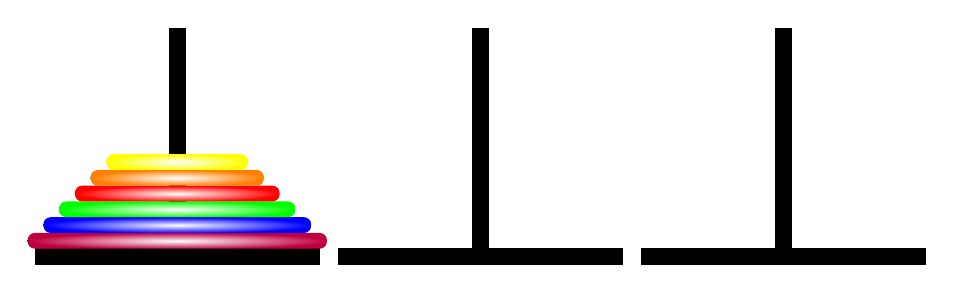
\begin{tikzpicture}
\draw[fill=black](0,0) rectangle +(3.6,0.2) (1.7,0) rectangle  +(0.2,3) (3.85,0) rectangle +(3.6,0.2) (5.55,0) rectangle +(0.2,3) (7.7,0) rectangle +(3.6,0.2) (9.4,0) rectangle +(0.2,3);
\shadedraw[inner color=white,outer color=purple,draw=none,rounded corners=0.6ex] (-0.1,0.2) rectangle +(3.8,0.2);
\shadedraw[inner color=white,outer color=blue,draw=none,rounded corners=0.6ex] (0.1,0.4) rectangle +(3.4,0.2);
\shadedraw[inner color=white,outer color=green,draw=none,rounded corners=0.6ex] (0.3,0.6) rectangle +(3.0,0.2);
\shadedraw[inner color=white,outer color=red,draw=none,rounded corners=0.6ex] (0.5,0.8) rectangle +(2.6,0.2);
\shadedraw[inner color=white,outer color=orange,draw=none,rounded corners=0.6ex] (0.7,1) rectangle +(2.2,0.2);
\shadedraw[inner color=white,outer color=yellow,draw=none,rounded corners=0.6ex] (0.9,1.2) rectangle +(1.8,0.2);
\end{tikzpicture}
\end{center}
\vspace*{-8pt}
\qquad\qquad\quad Peg 1\qquad\qquad
\qquad\quad\quad~ Peg 2\qquad\qquad
\qquad\quad\quad~ Peg 3
\newpage
Our goal is to find a \emph{recurrence relation} for the number $H_n$ of moves required to move a stack of $n$ disks from Peg 1 to Peg 2. Suppose we need $H_{n-1}$ moves to transfer the stack of $n-1$ disks to Peg 3:\\[5pt]
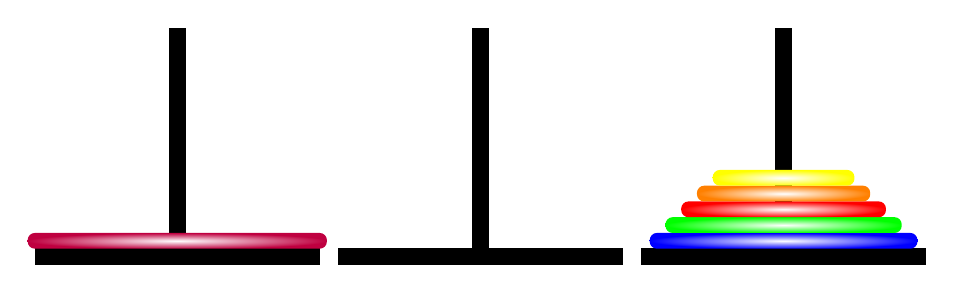
\begin{tikzpicture}
\draw[fill=black](0,0) rectangle +(3.6,0.2) (1.7,0) rectangle  +(0.2,3) (3.85,0) rectangle +(3.6,0.2) (5.55,0) rectangle +(0.2,3) (7.7,0) rectangle +(3.6,0.2) (9.4,0) rectangle +(0.2,3);
\shadedraw[inner color=white,outer color=purple,draw=none,rounded corners=0.6ex] (-0.1,0.2) rectangle +(3.8,0.2);
\shadedraw[inner color=white,outer color=blue,draw=none,rounded corners=0.6ex] (7.8,0.2) rectangle +(3.4,0.2);
\shadedraw[inner color=white,outer color=green,draw=none,rounded corners=0.6ex] (8,0.4) rectangle +(3.0,0.2);
\shadedraw[inner color=white,outer color=red,draw=none,rounded corners=0.6ex] (8.2,0.6) rectangle +(2.6,0.2);
\shadedraw[inner color=white,outer color=orange,draw=none,rounded corners=0.6ex] (8.4,0.8) rectangle +(2.2,0.2);
\shadedraw[inner color=white,outer color=yellow,draw=none,rounded corners=0.6ex] (8.6,1.0) rectangle +(1.8,0.2);
\end{tikzpicture}\\
\quad\qquad\quad Peg 1\qquad\qquad
\qquad\quad\quad~ Peg 2\qquad\qquad
\qquad\quad\quad~ Peg 3\\[4pt]
We can then transfer the largest disk to Peg 2, and then again use $H_{n-1}$ moves to transfer the other disks to Peg 2 on top of the largest disk. Thus,
\[H_n=2H_{n-1}+1,\qquad\qquad\quad
n\geq2,\qquad\qquad\quad H_1=1.\]
\newpage
\vspace*{11pt}
The first few terms of $(H_n)$ are
\[1,\,3,\,7,\,15,\,31,\,...\]
It seems that $H_n=2^n-1$. In fact, it is easy to prove this by induction: $H_1=2^1-1=1$, and if $H_{n-1}=2^{n-1}-1$, then
\[H_n=2H_{n-1}+1=2\cdot(2^{n-1}-1)+1=2^n-1.\]
\end{EXAMPLE}
\end{spacing}
\end{frame}
\begin{frame}[t,allowdisplaybreaks,allowframebreaks]{Fibonacci Numbers}
\begin{spacing}{1.1}
\begin{EXAMPLE}
Fibonacci originally posed the following problem in his \emph{Liber Abbaci} (Book of Calculations) in 1202:
\begin{quote}
A certain man put a pair of rabbits in a place surrounded on all
sides by a wall. How many pairs of rabbits can be produced from
that pair in a year if it is supposed that every month each pair
begets a new pair, which from the second month on becomes
productive?
\end{quote}
The solution to this problem leads to the sequence of Fibonacci numbers:
\begin{itemize}
  \item At the beginning of month 1, there is $f_1=1$ pair, which is not productive.
  \item At the beginning of month 2, there is still $f_2=1$ pair, which is now productive.
  \item At the beginning of month 3, there are now $f_3=2$ pairs, of which one is productive.
\newpage\vspace*{6pt}
  \item At the beginning of month 4, there are now $f_4=3$ pairs and the pair born in month 3 becomes productive.
  \item As the beginning of month 5, the number of pairs is equal to those of month 4, plus all those that were productive in month 4. These are all pairs that existed in month 3, since all of those will be productive in month 4. Hence, $f_5 = 3 + 2 = 5$.
  \item In general, at the beginning of every month the number of pairs of rabbits is equal to the number of pairs of the previous month, plus the number of pairs of two months ago, which have since become productive.
\end{itemize}
Hence, the classical Fibonacci sequence is
\[f_n=f_{n-1}+f_{n-2},\qquad\quad
n\geq2,\qquad\quad f_1=1,\qquad\quad
f_2=1.\]
\end{EXAMPLE}
\end{spacing}
\end{frame}
\begin{frame}[t]{Recurrence Relations}
\begin{spacing}{1.1}
In the proof of Lam\'{e}'s theorem we have used a basic estimate on the
Fibonacci sequence. We now discuss how to obtain this and similar
estimates in more general cases. This will enable us to study the
complexity of a wide class of algorithms.\\[5pt]
\begin{DEFINITION}
A \emph{recurrence relation} for a sequence $(a_n)$ is an equation of the form
\setcounter{equation}{0}
\begin{equation}\label{2.3.1}
a_n=f(a_0,\,...\,,a_{n-1}),\qquad\qquad\quad
\text{for}~n\geq k
\end{equation}
for some $k\in\N$.\\[5pt]
A sequence $(a_n)$ is called a solution to the recurrence relation if the terms
of the sequence satisfy \eqref{2.3.1}.\\[5pt]
Numbers $a_0,\,...\,,a_{k-1}$ that are given together with \eqref{2.3.1} are called \emph{initial conditions} for the recurrence relation.
\end{DEFINITION}
\end{spacing}
\end{frame}
\begin{frame}[c]{Existence and Uniqueness for Recurrence Relations}
\begin{spacing}{1.1}
\begin{LEMMA}
Let $a_0,\,...\,,a_{k-1}\in\R$ be given. Then there exists a unique sequence $(a_n)$ such that $a_n$ satisfies \eqref{2.3.1}.\\[6pt]
\end{LEMMA}
\begin{PROOF}
The existence of a unique sequence $(a_n)$ can be shown by strong induction in $n$: first, $a_0,\,...\,,a_{k-1}$ are given (and exist uniquely). Suppose that for some $n\geq k$ we know that $a_k,\,...\,,a_{n-1}$ exist uniquely such that \eqref{2.3.3} is satisfied with $n$ replaced by $k,\,...\,,n-1$, respectively. Then we define
\[a_n:=f(a_0,\,...\,,a_{n-1})\]
and we see that $a_n$ exists uniquely. This is precisely the procedure used to
verify that inductive definitions make sense.
\end{PROOF}
\end{spacing}
\end{frame}
\begin{frame}[t]{Linear Recurrence Relations}
\begin{spacing}{1.05}
\begin{DEFINITION}
A linear recurrence relation of degree $k\in\N\setminus\{0\}$ with constant (real) coefficients is a recurrence relation of the form
\begin{equation}\label{2.3.2}
a_n=c_1a_{n-1}+\cdots+c_ka_{n-k}+F(n)\qquad\quad
\text{for}~n\geq k,
\end{equation}
where $c_1,\,...\,,c_k\in\R,\,c_k\neq0$, and $F\!:\N\rightarrow\R$ is a sequence.\\[5pt]
If $F(n)=0$ for all $n$, \eqref{2.3.2} is said to be \emph{homogeneous}, otherwise \emph{inhomogeneous}.\\[5pt]
We will first treat the homogeneous case
\begin{equation}\label{2.3.3}
  a_n=c_1a_{n-1}+\cdots+c_ka_{n-k}.
\end{equation}
The basic approach for solving \eqref{2.3.3} is to make the ansatz
\begin{equation}\label{2.3.4}
  a_n=r^n
\end{equation}
and attempt to find a number $r\in\R$ such that \eqref{2.3.4} satisfies \eqref{2.3.3}.
\end{DEFINITION}
\end{spacing}
\end{frame}
\begin{frame}[t,allowdisplaybreaks,allowframebreaks]{Linear Homogeneous Recurrence Relations of Degree 2}
\begin{spacing}{1.05}
This leads to the \emph{characteristic equation} for \eqref{2.3.3},
\begin{equation}\label{2.3.5}
r^k-c_1r^{k-1}-\cdots-c_{k-1}r-c_k=0,
\end{equation}
whose left-hand side is called the characteristic polynomial. The solutions
of the characteristic equation are called characteristic roots of \eqref{2.3.3}.\\[5pt]
We will first treat recurrence relations of degree 2; those of degree 1 are
easily solvable, while those of higher degree imply discussing roots of
polynomials of degree $\geq3$, which is fairly involved.\\[5pt]
\begin{THEOREM}
Let $c_1,c_2\in\R$ such that $r^2-c_1r-c_2=0$ has two distinct roots $r_1$ and $r_2$. Then the sequence  $(a_n)$ is a solution of the recurrence relation $a_n=c_1a_{n-1}+c_2a_{n-2}$ if and only if
\begin{equation}\label{2.3.6}
a_n=\alpha_1\cdot r_1^n+\alpha_2\cdot r_2^n,\qquad\qquad\quad
\alpha_1,\alpha_2\in\R,~n\in\N.
\end{equation}
\end{THEOREM}
\begin{PROOF}
The proof is in two parts: first, we show that \eqref{2.3.6} actually solves the recurrence relation $a_n=c_1a_{n-1}+c_2a_{n-2}$; then, we show that every solution of $a_n=c_1a_{n-1}+c_2a_{n-2}$ is of the form \eqref{2.3.6}.\\[5pt]
Suppose that $a_n=\alpha_1r_1^n+\alpha_2r_2^n$. Since $r_1,r_2$ are roots of $r^2-c_1r-c_2=0$ we have
\begin{equation*}
  \begin{split}
     c_1a_{n-1}+c_2a_{n-2} &=c_1(\alpha_1r_1^{n-1}+\alpha_2r_2^{n-1})+c_2(\alpha_1r_1^{n-2}+\alpha_2r_2^{n-2}) \\
       &=\alpha_1r_1^{n-2}(c_1r_1+c_2)+\alpha_2r_2^{n-2}(c_1r_2+c_2) \\
       &=\alpha_1r_1^{n-2}r_1^2+\alpha_2r_2^{n-2}r_2^2 \\
       &=a_n
  \end{split}
\end{equation*}
so the recurrence relation is satisfied. This shows that \eqref{2.3.6} solves the recurrence relation.
\newpage
\alert{Proof (continued).}\\
Now let $(a_n)$ be a solution to the recurrence relation. By Lemma 2.3.4 this sequence is unique and determined by $a_0$ and $a_1$. We thus need to show that we can find $\alpha_1$ and $\alpha_2$ such that
\[a_0=\alpha_1+\alpha_2,\qquad\qquad\qquad
a_1=\alpha_1r_1+\alpha_2r_2.\]
If this is possible, it follows that $a_n=\alpha_1r_1^n+\alpha_2r_2^n$ for all $n\in\N$. A simple calculation yields
\[\alpha_1=\frac{a_1-a_0r_2}{r_1-r_2},\qquad\qquad
\qquad \alpha_2=\frac{a_0r_1-a_1}{r_1-r_2}\]
so
\begin{equation*}
  a_n=\frac{a_1-a_0r_2}{r_1-r_2}r_1^n+\frac{a_0r_1-a_1}{r_1-r_2}r_2^n.
\end{equation*}
\end{PROOF}
\newpage
\begin{EXAMPLE}
The Fibonacci sequence satisfies $f_0=0,f_1=1$ and $f_n=f_{n-1}+f_{n-2}$. Setting $f_n=r^n$, we obtain
\[r^n-r^{n-1}-r^{n-2}=0\]
or
\[r^2-r-1=0.\]
The characteristic roots are
\[r_{1,2}=\frac{1\pm\sqrt{5}}{2},\]
so, finding suitable constants to satisfy the initial conditions, we obtain
\[f_n=\frac{1}{\sqrt{5}}\left(\frac{1+\sqrt{5}}{2}\right)^n-\frac{1}{\sqrt{5}}
\left(\frac{1-\sqrt{5}}{2}\right)^n.\]
\end{EXAMPLE}
\end{spacing}
\end{frame}
\begin{frame}[t]{Homogeneous Recurrence Relations of Degree 2}
\begin{spacing}{1}
If there is only a single characteristic root of multiplicity 2, then we have
the following result:\\[4pt]
\begin{THEOREM}
Let $c_1,c_2\in\R,\,c_2\neq0$ such that $r^2-c_1r-c_2=0$ has a single roots $r_0$. Then the sequence $(a_n)$ is a solution of the recurrence relation $a_n=c_1a_{n-1}+c_2a_{n-2}$ if and only if
\[a_n=\alpha_1\cdot r_0^n+\alpha_2\cdot nr_0^n,\qquad\qquad
\alpha_1,\alpha_2\in\R,\:n\in\N.\]
The proof is left to the exercises.\\[4pt]
\begin{EXAMPLE}
We consider the recurrence relation $a_n=6a_{n-1}-9a_{n-2}$ with initial conditions $a_0=1$ and $a_1=6$. There is only one characteristic root, $r=3$. Then
\[a_n=\alpha_13^n+\alpha_2n3^n.\]
To find $\alpha_1,\alpha_2$ we use $a_0=\alpha_1=1$ and $a_1=3\alpha_1+3\alpha_2=6$. This gives
\[a_n=(n+1)3^n.\]
\end{EXAMPLE}
\end{THEOREM}
\end{spacing}
\end{frame}
\begin{frame}[t,allowdisplaybreaks,allowframebreaks]{Homogeneous Recurrence Relations of Degree $k$}
\begin{spacing}{1.05}
We will no prove the following result, which generalizes the solution ansatz
to recurrence relations of degree $k$:\\[4pt]
\begin{THEOREM}
Let $c_1,c_2,\,...\,,c_k\in\R$ such that
\[r^k-c_1r^{k-1}-\cdots-c_{k-1}r-c_k=0\]
has $t$ distinct roots $r_1,\,...\,,r_t$ with multiplicities $m_1,\,...\,,m_t$, respectively. Then the sequence $(a_n)$ is a solution of the recurrence relation $a_n=c_1a_{n-1}+c_2a_{n-2}+\cdots+c_ka_{n-k}$ if and only if
\begin{equation*}
  \begin{split}
     a_n =&\,(\alpha_{1,0}+\alpha_{1,1}n+\cdots+\alpha_{1,m_1-1}n^{m_1-1})\cdot r_1^n \\
       &+(\alpha_{2,0}+\alpha_{2,1}n+\cdots+\alpha_{2,m_2-1}n^{m_2-1})\cdot r_2^n \\
       &+\cdots+(\alpha_{t,0}+\alpha_{t,1}n+\cdots+\alpha_{t,m_t-1}n^{m_t-1})\cdot r_t^n,~n\in\N.
  \end{split}
\end{equation*}
where $\alpha_{i,j}\in\R,~1\leq i\leq t,~0\leq j\leq m_i-1$.
\end{THEOREM}
\end{spacing}
\newpage
\begin{spacing}{0.8}
\begin{EXAMPLE}
We want to solve
\[a_n=-3a_{n-1}-3a_{n-2}-a_{n-3},\qquad\quad
a_0=1,\qquad\quad a_1=-2,\qquad\quad
a_2=-1.\]
The characteristic root is found from
\[r^3+3r^2+3r+1=(r+1)^3=0\]
so we have $r=-1$ with multiplicity 3. The solution of the recurrence relation is then
\[a_n=\alpha_{1,0}(-1)^n+\alpha_{1,1}n(-1)^n+\alpha_{1,2}n^2(-1)^n.\]
To find the constants we solve
\begin{align*}
  a_0 &=\alpha_{1,0}=1, \\
  a_1 &=-\alpha_{1,0}-\alpha_{1,1}-\alpha_{1,2}=-2, \\
  a_2 &=\alpha_{1,0}+2\alpha_{1,1}+4\alpha_{1,2}=-1
\end{align*}
to obtain
\[a_n=(1+3n-2n^2)(-1)^n.\]
\end{EXAMPLE}
\end{spacing}
\end{frame}
\begin{frame}[t,allowdisplaybreaks,allowframebreaks]{Inhomogeneous Recurrence Relations}
\begin{spacing}{1.05}
In the inhomogeneous case we want to solve
\begin{equation}\label{2.3.7}
a_n=c_1a_{n-1}+\cdots+c_ka_{n-k}+F(n)\qquad\qquad
\text{for}~n\geq k
\end{equation}
with constants $c_1,\,...\,,c_k\in\R$. The general solution to \eqref{2.3.7} will be the
sum of a particular solution and solutions of the associated homogeneous
equation. This is analogous to the solution of inhomogeneous systems of
linear algebraic equations or of inhomogeneous systems of linear ordinary
differential equations.\\[5pt]
\begin{THEOREM}
If $(a_n^{\text{part}})$ is a particular solution of \eqref{2.3.7}, then every solution is of the form $(a_n)=(a_n^{\text{part}}+a_n^{\text{hom}})$, where $(a_n^{\text{hom}})$ solves \eqref{2.3.7} with $F(n)=0$ for all $n$.\\[5pt]
We omit the proof, which is similar to the corresponding statements for
systems of ODEs or linear equations.
\end{THEOREM}
\newpage
\begin{EXAMPLE}
Consider the recurrence equation $a_n=3a_{n-1}+2n$ with initial value $a_1=3$. The associated homogeneous equation $a_n=3a_{n-1}$ has general solution $a_n^{\text{hom}}=\alpha\cdot3^n$. A particular solution can be found by educated guessing: since $F(n)=2n$ is a polynomial of degree 1, try setting $a_n^{\text{part}}=cn+d$ for $c,d\in\R$ to be determined. Then
\[cn+d=3(c(n-1)+d)+2n\qquad\quad\Rightarrow\qquad\quad
(2+2c)n+(2d-3c)=0,\]
so we have $c=-1$ and $d=-3/2$. Thus,
\[a_n=\alpha\cdot 3^n-n-3/2\]
solves the recurrence relation. The initial condition $a_1=3$ then gives $\alpha=11/6$, so
\[a_n=\frac{11}{2}3^{n-1}-n-\frac{3}{2}.\]
\end{EXAMPLE}
 \\[11pt]
It is no accident that in this example we were able to find a particular
solution by guessing it to be a polynomial. In fact, if $F(n)$ is an
exponential function, then we can also find a particular solution of
exponential form. In fact, the following theorem holds.
\end{spacing}
\newpage
\begin{spacing}{0.6}
\begin{THEOREM}
Consider the inhomogeneous equation \eqref{2.3.7} with
\[F(n)=s^n\sum_{j=0}^{t}b_jn^j,\qquad\qquad\qquad
s,b_0,\,...\,,b_t\in\R.\]
A particular solution to \eqref{2.3.7} then has the following form:
\begin{itemize}
  \item If $s$ is not a characteristic root of the associated homogeneous equation, then there exist numbers $p_0,\,...\,,p_t\in\R$ such that
      \[a_n^{\text{part}}=s^n\sum_{j=0}^{t}p_jn^j.\]
  \item If $s$ is a characteristic root of multiplicity $m$, then there exist numbers $p_0,\,...\,,p_t\in\R$ such that
      \[a_n^{\text{part}}=n^ms^n\sum_{j=0}^{t}p_jn^j.\]
\end{itemize}
\end{THEOREM}
\newpage
\begin{EXAMPLE}
Consider the recurrence relation
\[a_n=6a_{n-1}-9a_{n-2}+F(n),\]
where we are interested in the cases
\begin{enumerate}[1.]
  \item $F(n)=3^n$,
  \item $F(n)=n3^n$,
  \item $F(n)=n^22^n$,
  \item $F(n)=(n^2+1)3^n$.
\end{enumerate}
The associated homogeneous equation is $a_n=6a_{n-1}-9a_{n-2}$ which has a single characteristic root $r=3$ of multiplicity 2. We then have particular solutions of the following forms:
\begin{enumerate}[1.]
  \item $a_n^{\text{part}}=p_0n^23^n$,
  \item $a_n^{\text{part}}=(p_0+p_1n)n^23^n$,
  \item $a_n^{\text{part}}=(p_0+p_1n+p_2n^2)2^n$,
  \item $a_n^{\text{part}}=(p_0+p_1n+p_2n^2)n^23^n$.
\end{enumerate}
\end{EXAMPLE}
\end{spacing}
\end{frame}
\begin{frame}[t,allowdisplaybreaks,allowframebreaks]{Divide-and-Conquer Algorithms}
\begin{spacing}{1.1}
The principle of ``divide and conquer'', (originating from \emph{divide et impera},
divide and rule, in Latin) goes back to the ancient Romans who used
political, economic and military means to break up alliance of opponents
or concentrations of power so that each part was less powerful than
themselves.\\[5pt]
In computer algorithms, \emph{divide-and-conquer} algorithms are those that
break up a problem into several smaller instances and tackle each instance
separately. They are similar to recursive algorithms, but ``multi-branched'',
i.e., referring to several instances of themselves, not just one, with smaller
input.\\[5pt]
We are interested in analyzing the time complexity of divide-and-conquer
algorithms. It turns out that recurrence relations are well-suited to
describing the number of steps needed for such an algorithm to complete
and that we can find quite general formulas for big-Oh estimates for many
classes of algorithms.
\end{spacing}
\newpage
\begin{spacing}{0.91}
\begin{EXAMPLES}
\begin{itemize}
  \item[(i)] The Binary Search Algorithm 2.1.9 reduces the problem of locating an element of a list to locating it in a list of half the length. Two comparisons are needed to do this, one to determine which half-list to search, the other to determine whether any terms remain in the list. Therefore, the number of comparisons needed to search a list of length $n$ is given by
      \[f(n)=f(n/2)+2.\]
      Since only one list of length $n/2$ is searched, this is actually a recursive algorithm, a special case of a divide-and-conquer algorithm.
  \item[(ii)] A divide-and-conquer algorithm to find the minimum and maximum of a list of length $n = 2k$ might split the list into two equally sized sublists, find the minimum and maximum in each sublist and compare the values of the two sublists. The number of comparisons needed is then given by
      \[f(n)=2f(n/2)+2.\]
\newpage
  \item[(iii)] The \emph{Karatsuba algorithm} is a divide-and-conquer algorithm for integer multiplication which is faster than Algorithm 2.2.7. Suppose that $a$ and $b$ are integers with binary representations of length $2n$ (adding leading zeroes if necessary),
      \[a=(a_{2n-1}\,...\,a_1a_0)_2,\qquad\qquad\quad
      b=(b_{2n-1}\,...\,b_1b_0)_2.\]
      Setting
      \begin{align*}
        A_0 &=(a_{n-1}\,...\,a_0)_2, & A_1 &=(a_{2n-1}\,...\,a_n)_2, \\
        B_0 &=(b_{n-1}\,...\,b_0)_2, & B_1 &=(b_{2n-1}\,...\,b_n)_2
      \end{align*}
      we can write
      \[a=2^nA_1+A_0,\qquad\qquad\quad
      b=2^nB_1+B_0.\]
\newpage
      Then
      \[a\cdot b=(2^{2n}+2^n)A_1B_1+2^n(A_1-A_0)(B_0-B_1)+(2^n+1)A_0B_0,\]
      so the multiplication of two integers of length $2n$ is reduced to summing three multiplications of integers of length $n$. The number of operations required for the multiplications by powers of 2 (shifts in the binary expansion) and addition are proportional to $n$, so the total number of operations is given by
      \[f(2n)=3f(n)+Cn\]
      for some $C\in\N$.
  \item[(iv)] The Merge Sort Algorithm 2.1.27 reduces the problem of sorting a list with n elements to that of sorting two lists with $n/2$ elements. It then uses fewer than n comparisons to merge the two sorted lists. Therefore, it uses fewer than $M(n)$ comparisons, where
      \[M(n)=2M(n/2)+n.\]
\end{itemize}
\end{EXAMPLES}
\end{spacing}
\end{frame}
\begin{frame}[t,allowdisplaybreaks,allowframebreaks]{Time Complexity of Divide-and-Conquer Algorithms}
\begin{spacing}{1}
\begin{THEOREM}
Let $f$ be an increasing function that satisfies the recurrence relation
\[f(n)=af(n/b)+c,\qquad\qquad
a\geq1,~b\in\N\setminus\{0,1\},~c>0\]
whenever $n$ is divisible by $b$. Then
\[f(n)=\begin{cases}
         O(n^{\log_ba}), & \mbox{if } a>1,\\
         O(\log n), & \mbox{if } a=1.
       \end{cases}\]
Furthermore, whenever $a>1$ and $n=b^k$ for some $k\in\Z_+$,
\begin{equation}\label{2.3.8}
  f(n)=C_1n^{\log_ba}+C_2
\end{equation}
with
\[C_1=f(1)+\frac{c}{a-1},\qquad\qquad\qquad
C_2=-\frac{c}{a-1}.\]
\end{THEOREM}
\end{spacing}
\begin{PROOF}
\begin{spacing}{0.9}
We first note that if $f(n)=af(n/b)+g(n)$ for some function $g$,
\begin{equation*}
  \begin{split}
     f(n) &=af\left(\frac{n}{b}\right)+g(n)=a\left(af\left(\frac{n}{b^2}\right)+g\left(\frac{n}{b}\right)\right)+g(n) \\
       &=a^2f\left(\frac{n}{b^2}\right)+ag\left(\frac{n}{b}\right)+g(n) \\
       &\vdots \\
       &=a^kf\left(\frac{n}{b^k}\right)+\sum_{j=0}^{k-1}a^jg\left(\frac{n}{b^j}\right)
  \end{split}
\end{equation*}
for any $k\in\N$. If $n=b^k$ for some $k\in\N$, we obtain
\begin{equation}\label{2.3.9}
f(n)=a^kf(1)+\sum_{j=0}^{k-1}a^jg\left(\frac{n}{b^j}\right).
\end{equation}
\newpage
\alert{Proof (continued).}\\
We will now prove the various statements of the theorem.
\begin{itemize}
  \item[(i)] Suppose that $a=1$. If $n=b^k$ for some $k\in\N$, \eqref{2.3.9} gives
      \[f(n)=f(1)+c\cdot k=f(1)+c\cdot\log_bn=O(\log n).\]
      Furthermore, if $b^k<n<b^{k+1}$ for some $k\in\N$ we use that $f$ is increasing to obtain
      \[f(n)\leq f(b^{k+1})=f(1)+c(k+1)=f(1)+c+c\cdot\log_bn=O(\log n).\]
      This proves the statement of the theorem for $a=1$.
\end{itemize}
\newpage
\alert{Proof (continued).}\\
\begin{itemize}
  \item[(ii)] Now let $a>1$ and $n=b^k$. Then \eqref{2.3.9} gives
      \begin{equation*}
        \begin{split}
           f(n) &=a^kf(1)+c\sum_{j=0}^{k-1}a^j=a^kf(1)+c\frac{a^k-1}{a-1} \\
             &=a^k\left(f(1)+\frac{c}{a-1}\right)-\frac{c}{a-1} \\
             &=C_1n^{\log_ba}+C_2,
        \end{split}
      \end{equation*}
      where we have used $a^k=a^{\log_bn}=n^{\log_ba}$. This proves \eqref{2.3.8}. If $b^k<n<b^{k+1}$ for some $k\in\N$ we use that $f$ is increasing to obtain
      \[f(n)\leq f(b^{k+1})=a^k\left(af(1)+\frac{ac}{a-1}\right)-\frac{c}{a-1}
      =O(n^{\log_ba}).\]
\end{itemize}
\end{spacing}
\end{PROOF}
\newpage
\begin{spacing}{1}
We now apply Theorem 2.3.17 to the first two of the Examples 2.3.16:\\[5pt]
\begin{EXAMPLES}
\begin{enumerate}[(i)]
  \item The comparisons needed by the Binary Search algorithm satisfy $f(n)=f(n/2)+2$, so
      \[f(n)=O(\log n).\]
  \item The comparisons needed for finding the minimum and maximum of a list of integers satisfy $f(n)=2f(n/2)+2$, so
      \[f(n)=O(n^{\log_22})=O(n).\]
\end{enumerate}
\vspace*{9pt}
In order to treat the other examples, we need a more general theorem.
\end{EXAMPLES}
\end{spacing}
\end{frame}
\begin{frame}[t,allowdisplaybreaks,allowframebreaks]{The Master Theorem}
\begin{spacing}{1}
The following result is called the ``Master Theorem'' because it can be
used to obtain the time complexity of many divide-and-conquer
algorithms. There exist more powerful variants that give big-$\Theta$ estimates.\\[5pt]
\stepcounter{zhuo}
\alert{2.3.19. Master Theorem.} Let $f$ be an increasing function that satisfies the recurrence relation
\[f(n)=af(n/b)+cn^d,\qquad\quad a\geq1,~b\in\N\setminus\{0,1\},~c>0,~d\geq0\]
whenever $n=b^k$. Then
\[f(n)=\begin{cases}
         O(n^d)  & \mbox{if } a<b^d, \\
         O(n^d\log n)  & \mbox{if } a=b^d, \\
         O(n^{\log_ba})  & \mbox{if } a>b^d,
       \end{cases}\]
The proof of the Master Theorem is relegated to the exercises.
\newpage
We now apply the Master Theorem to the remaining two Examples 2.3.16:\\[5pt]
\begin{EXAMPLES}
\begin{enumerate}[(i)]
  \item The number of comparisons needed by the Merge Sort algorithm is bounded by $M(n)$, where $M(n)=2M(n/2)+n$, so
      \[M(n)=O(n\log n).\]
  \item The number of operations needed for the fast integer multiplication satisfies $f(n)=3f(n/2)+Cn$, so
      \[f(n)=O(n^{\log_23})=O(n^{1.585}).\]
      This is a significant improvement on the ``classical'' algorithm, which uses $O(n^2)$ operations.
\end{enumerate}
\end{EXAMPLES}
\end{spacing}
\end{frame}
\subsection{Combinatorics}
\begin{frame}[c] \begin{spacing}{2.5}
\tableofcontents[sectionstyle=hide,subsectionstyle=show/shaded/hide] \end{spacing}
\end{frame}
\begin{frame}[t]{Counting}
\begin{spacing}{0.9}
In mathematics, as well as in applications, it is important to know how to
count. The act of counting can be described as finding the ``number of
elements'' in a set. How is this done? In the final analysis, by comparing
one set with a set where the number of elements is known.\\[5pt]
For example, consider the set of bit strings of length 2,
\[A=\{00,01,10,11\}.\]
Counting the elements in the set is done as follows:
\begin{align*}
  00 &\rightarrow 1,  \\
  01 &\rightarrow 2,  \\
  10 &\rightarrow 3,  \\
  11 &\rightarrow 4.
\end{align*}
We have found a one-to-one correspondence between the element of $A$ and
the elements of the set $\{1,2,3,4\}$. We conclude that $A$ has 4 elements.
\end{spacing}
\end{frame}
\begin{frame}[t,allowdisplaybreaks,allowframebreaks]{Cardinality}
\begin{spacing}{0.9}
We can make this more precise as follows:\\[4pt]
\begin{DEFINITION}
Let $A,B$ be arbitrary sets.
\begin{enumerate}[(i)]
  \item The sets $A$ and $B$ have \emph{equal cardinality} if there exists a bijective function $\varphi\!:A\rightarrow B$. In this case we write
      \[\text{card}\,A=\text{card}\,B.\]
  \item The set $A$ is said to have a \emph{cardinality no greater than B} if there exists an injective function $\varphi\!:A\rightarrow B$. In this case we write
      \[\text{card}\,B\geq\text{card}\,A.\]
  \item The set $B$ is said to have a \emph{cardinality strictly greater than A} if there exists an injective function $\varphi\!:A\rightarrow B$ but there does not exist a bijective function from $A$ to $B$. In this case we write
      \[\text{card}\,B>\text{card}\,A.\]
\end{enumerate}
\end{DEFINITION}
\end{spacing}
\newpage
\begin{spacing}{1.05}
\begin{REMARKS}
Although we want to think of cardinality as meaning
``number of elements'', we have not actually defined this. In fact, we have
not even stated what cardinality \emph{actually} is. We have only defined what it
means that two sets have equal cardinality.\\[5pt]
We are very careful with our definitions because a set may have an
``infinite number of elements'' and in fact it turns out that there are
\emph{different sizes of infinity}! Therefore, terms such as ``number of elements''
need to be handled with extreme care.\\[5pt]
This also means that ``seemingly obvious'' statements require non-trivial
proofs or further assumptions. For example, the fact that
\[\text{card}\,A\geq\text{card}\,B\qquad\wedge
\qquad\text{card}\,B\geq\text{card}\,A\qquad
\Rightarrow\qquad\text{card}\,A=\text{card}\,B\]
is not trivial (\emph{Cantor-Schr\"{o}der-Bernstein Theorem}) and is in fact not
accepted by a minority of mathematicians.
\end{REMARKS}
\end{spacing}
\end{frame}
\begin{frame}[t]{Finite, Infinite, Countable and Uncountable Sets}
\begin{spacing}{1.05}
We can define
\setcounter{equation}{0}
\begin{equation}\label{2.4.1}
A\sim B\qquad\qquad\quad\Leftrightarrow\qquad
\qquad\quad\text{card}\,A=\text{card}\,B
\end{equation}
and this is in fact an equivalence relation (check this!). The set of all
possible cardinalities of a set is equal to the set of equivalence classes
induced by \eqref{2.4.1}.\\[5pt]
\begin{DEFINITION}
Let $A$ be a set and $\sim$ the equivalence relation \eqref{2.4.1}.
\begin{enumerate}[(i)]
  \item If $A\sim\{1,2,\,...\,,n\}$ for some $n\in\N$, we write $\text{card}\,A=n$.\\ $A$ is said to be \emph{finite}.
  \item If $A\sim\N$, we write $\text{card}\,A=\aleph_0$.\\ $A$ is said to be \emph{countably infinite}.
\end{enumerate}
If $A$ is not finite, $A$ is said to be \emph{infinite}.\\[5pt]
If $A$ is finite or countably infinite, $A$ is said to be \emph{countable}, otherwise $A$ is \emph{uncountable}.
\end{DEFINITION}
\end{spacing}
\end{frame}
\begin{frame}[t,allowdisplaybreaks,allowframebreaks]{Cardinalities of Infinite Sets}
\begin{spacing}{1.05}
At this point, we rapidly start to leave the confines of naive set theory and
enter territory where each statement has to be preceded by saying which
axioms of set theory need to be assumed for the statement to be true.\\[5pt]
For example, supposing a general, set-theoretic \emph{well-ordering principle}, the
set of possible cardinalities can be ordered and the cardinalities of the
infinite sets denoted by
\[\aleph_0<\aleph_1<\,...\]
(Again, there are mathematicians who dispute this because they do not
accept the general well-ordering principle.) Then it is not difficult to show
that $\N$ is the ``smallest'' infinite set and is assigned the cardinality $\aleph_0$, as
we have done.\\[5pt]
We will prove that $\text{card}\R>\aleph_0$ (but our proof is not accepted by
everyone$...$). Then the question is whether
\[\text{card}\R=\aleph_1?\]
\newpage
In other words, is there an infinite set with ``more'' elements than $\N$ but
``fewer'' elements than $\R$? Supposing that $\text{card}\R=\aleph_1$ is known as the
\emph{continuum hypothesis}.\\[6pt]
The situation gets even more confusing: using commonly accepted axioms
of set theory (the ZFC axioms introduced to eliminate the Russell paradox
and the problems with naive set theory),
\begin{quote}
It has been proven that the continuum hypothesis can be neither
proven nor disproven within the ZFC axioms, assuming that the
ZFC axioms are consistent.
\end{quote}
Hence, a choice can be made: either $\text{card}\R=\aleph_1$ or $\text{card}\R>\aleph_1$. Either
choice is acceptable and leads to a ``consistent'' branch of mathematics.
Since human intuition fails to tell us which choice is ``correct'' and
mathematics can (provably!) not provide an answer, the choice is
essentially arbitrary.
\end{spacing}
\end{frame}
\begin{frame}[t,allowdisplaybreaks,allowframebreaks,fragile]{Counting and Cardinality}
\begin{spacing}{1.1}
\begin{EXAMPLES}
\begin{itemize}
  \item[1.] The set of bit strings of length 2, $M=\{00,01,10,11\}$ is finite and has cardinality $\text{card}\,M=4$, because we can define the map $\varphi\!:M\rightarrow\{1,2,3,4\}$ by
      \[00\mapsto1,\qquad\quad01\mapsto2,\qquad\quad
      10\mapsto3,\qquad\quad11\mapsto4.\]
      It is clear that this map is bijective, so we have counted $M$. (We say that we have counted $M$ when we have found a bijection $\varphi$.)
  \item[2.] The set of even natural numbers $2\N=\{n\in\N\!:n=2k,\,k\in\N\}$is countably infinite; we simply define the bijection
      \[\varphi\!:n\mapsto\frac{n}{2}.\]
\end{itemize}
\end{EXAMPLES}
\newpage
\begin{EXAMPLE}
The positive rationals are countably infinite:
\begin{center}
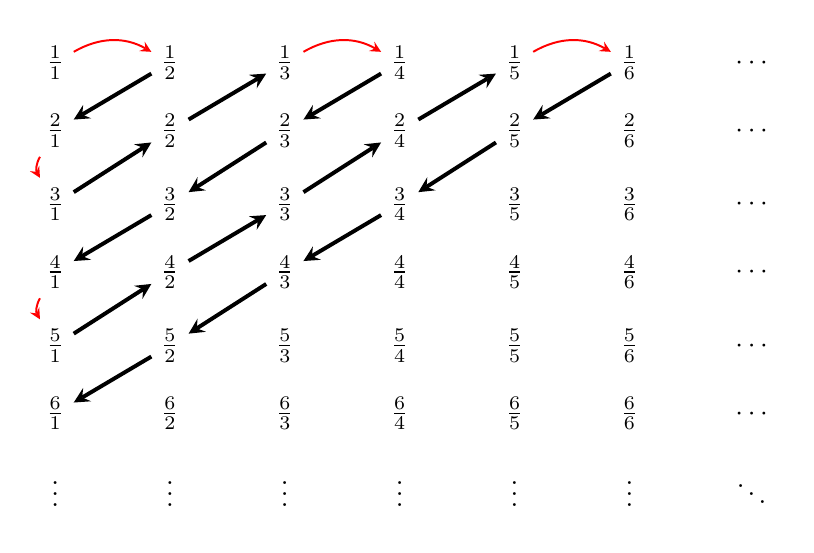
\begin{tikzpicture}[>=stealth,->]
\matrix (mat1) [matrix of math nodes]
{
  |(A)|\frac{1}{1} &[1cm] |(B)|\frac{1}{2} &[1cm] |(C)|\frac{1}{3} &[1cm] |(D)|\frac{1}{4} &[1cm] |(E)|\frac{1}{5} &[1cm] |(F)|\frac{1}{6} &[1cm] \cdots \\[6pt]
  |(G)|\frac{2}{1} & |(H)|\frac{2}{2} & |(I)|\frac{2}{3} & |(J)|\frac{2}{4} & |(K)|\frac{2}{5} & \frac{2}{6} & \cdots \\[8pt]
  |(L)|\frac{3}{1} & |(M)|\frac{3}{2} & |(N)|\frac{3}{3} & |(O)|\frac{3}{4} & \frac{3}{5} & \frac{3}{6} & \cdots \\[6pt]
  |(P)|\frac{4}{1} & |(Q)|\frac{4}{2} & |(R)|\frac{4}{3} & \frac{4}{4} & \frac{4}{5} & \frac{4}{6} & \cdots \\[8pt]
  |(S)|\frac{5}{1} & |(T)|\frac{5}{2} & \frac{5}{3} & \frac{5}{4} & \frac{5}{5} & \frac{5}{6} & \cdots \\[6pt]
  |(U)|\frac{6}{1} & \frac{6}{2} & \frac{6}{3} & \frac{6}{4} & \frac{6}{5} & \frac{6}{6} & \cdots \\[6pt]
  \vdots & \vdots & \vdots & \vdots
   & \vdots & \vdots & \ddots \\
};
\begin{scope}
  \draw[red,line width=0.25mm](A) to [bend left] node [midway] {}(B);
  \draw[red,line width=0.25mm](C) to [bend left] node [midway] {}(D);
  \draw[red,line width=0.25mm](E) to [bend left] node [midway] {}(F);
  \draw[red,line width=0.25mm](G) to [bend right] node [midway] {}(L);
  \draw[red,line width=0.25mm](P) to [bend right] node [midway] {}(S);
  \draw[line width=0.5mm](B) -- node [midway] {}(G);
  \draw[line width=0.5mm](H) -- node [midway] {}(C);
  \draw[line width=0.5mm](D) -- node [midway] {}(I);
  \draw[line width=0.5mm](J) -- node [midway] {}(E);
  \draw[line width=0.5mm](F) -- node [midway] {}(K);
  \draw[line width=0.5mm](L) -- node [midway] {}(H);
  \draw[line width=0.5mm](I) -- node [midway] {}(M);
  \draw[line width=0.5mm](N) -- node [midway] {}(J);
  \draw[line width=0.5mm](K) -- node [midway] {}(O);
  \draw[line width=0.5mm](M) -- node [midway] {}(P);
  \draw[line width=0.5mm](Q) -- node [midway] {}(N);
  \draw[line width=0.5mm](O) -- node [midway] {}(R);
  \draw[line width=0.5mm](S) -- node [midway] {}(Q);
  \draw[line width=0.5mm](R) -- node [midway] {}(T);
  \draw[line width=0.5mm](T) -- node [midway] {}(U);
\end{scope}
\end{tikzpicture}
\end{center}
\end{EXAMPLE}
\end{spacing}
\end{frame}
\begin{frame}[t,allowdisplaybreaks,allowframebreaks]{Uncountability of the Set of Bit Strings}
\begin{spacing}{1.1}
Note that on the one hand there is a bijection $\N\rightarrow\Omega$, where $\Omega=\{p/q\in\Q\!:q=1,\,p\in\Z\}$ is a strict subset of $\Q$, while on the other hand there is a bijection $\N\rightarrow\Q$. According to our definition of cardinality, the ``number of elements'' of $\Omega$ and $\Q$ are therefore equal. This contradicts the classical principle that ``the size of the whole can not be equal to the size of a part''.\\[5pt]
We next give a famous result of George Cantor concerning the set $T$ of bit
strings of infinite length. We may regard such strings as infinite sequences
whose entries take on only the values zero and one, i.e.,
\[T=\big\{(a_n):\N\rightarrow\{0,1\}\big\}.\]
\begin{THEOREM}
The set $T$ has cardinality greater than $\aleph_0$, i.e., is uncountable.
\end{THEOREM}
\end{spacing}
\newpage
\begin{spacing}{1}
\begin{PROOF}
The following method of proof is known as \emph{Cantor's diagonal argument.} Suppose that $T$ is countable. Then we can find a sequence $(x_n)\!:\N\to\C$ and list the elements of this sequence, e.g.,
\begin{align*}
  x_0 &=(0,0,0,0,0,0,0,\,...), \\
  x_1 &=(1,1,1,1,1,1,1,\,...), \\
  x_2 &=(0,1,0,1,0,1,0,\,...), \\
  x_3 &=(1,0,1,0,1,0,1,\,...), \\
      &\vdots
\end{align*}
We now define
\[y=(y_n)=(1,0,1,1,\,...)\]
such that $y_n\neq(x_n)_n$. Since $y\neq x_n$ for all $n$, we arrive at a contradiction.
\end{PROOF}
\end{spacing}
\end{frame}
\begin{frame}[t]{Uncountability of the Set of Real Numbers}
\begin{spacing}{1.1}
\begin{COROLLARY}
The set $\R$ of real numbers is uncountable.\\[4pt]
\end{COROLLARY}
\begin{PROOF}
We first show that $\text{card}\,\R=\text{card}(0,1)$, where $(0,1)\subset\R$ is the unit interval, by exhibiting a suitable bijection:
\[\varphi\!:(0,1)\to\R,\qquad\qquad\qquad
\varphi(x)=\tan\left(\frac{(2x-1)\pi}{2}\right)\]
Next, we represent every number in the interval $[0,1]$ in base 2, so that its binary digits may be considered to be a bit string. There is a small
technical difficulty at this point: two different bit strings can represent the
same real number, e.g., $0.0111\cdots=0.10000\,....$ However, because there are only countably many such numbers (why?) they can be accounted for
separately. We omit the details here. Then, since $T$ is uncountable, so is
$\R$.
\end{PROOF}
\end{spacing}
\end{frame}
\begin{frame}[t,allowdisplaybreaks,allowframebreaks]{Cardinality of Power Sets}
\begin{spacing}{1.2}
\begin{THEOREM}
Let $M$ be a finite set with $\text{card}\,M=n$. Then the power set of $M,\mathcal{P}(M)$, has cardinality $2^n$.\\[5pt]
\end{THEOREM}
\begin{PROOF}
Assume that the elements of $M$ are numbered, writing $M=\{a_1,\,...\,,a_n\}$. We associate any element of $\mathcal{P}(M)$ with a bit string of length $n$ as follows: an element $S\in\mathcal{P}(M)$ is a subset $S\subset M$. We associate to $S$ the bit string of length $n$ where the $i$th bit is 1 if $a_i\in S$ and 0 if $a_i\notin S$. Thus we obtain a bijective map from $\mathcal{P}(M)$ to the bit strings of length $n$.\\[6pt]
Now a bit string of length $n$ is the binary representation of a number between 0 and $2^n-1$. We associate to each bit string this number plus 1, obtaining a bijection $\mathcal{P}(M)\to\{1,\,...\,,2^n\}$.
\end{PROOF}
\newpage
\begin{REMARK}
The same argument shows that
\[\text{card}\,\mathcal{P}(\N)=\text{card}\,T=\text{card}\,\R.\]
More generally, a theorem due to Cantor states that
\[\text{card}\,\mathcal{P}(A)>\text{card}\,A\]
for any set $A$ and hence
\[\text{card}\,P(\R)>\text{card}\,\R.\]
We conclude that the set of functions $f:\R\to\R$ has a larger cardinality than $\R$.
\end{REMARK}
\end{spacing}
\end{frame}
\begin{frame}[t,allowdisplaybreaks,allowframebreaks]{Cardinality of Cartesian Products}
\begin{spacing}{1.1}
\begin{THEOREM}
Let $M,N$ be finite sets with $\text{card}\,M=m,\,\text{card}\,N=n$. Then the cartesian product of $M$ and $N$, $M\times N$, has cardinality $m\cdot n$.\\[5pt]
\end{THEOREM}
\begin{PROOF}
Suppose that $M=\{a_1,\,...\,,a_m\}$ and $N=\{b_1,\,...\,,b_n\}$. Then we define
\[\varphi\!:\,M\times N\to\{1,\,...\,,m\cdot n\},\qquad\qquad\quad
(a_i,b_j)\mapsto(i-1)n+j.\]
The inverse map is
\[\varphi^{-1}\!:\{1,\,...\,,m\cdot n\}\to M\times N,\qquad x\mapsto(a_{1+((x-1)\text{div}\,n)},b_{1+((x-1)\mod n)}),\]
and it is then easy to see that $\varphi$ is bijective.
\end{PROOF}
\end{spacing}
\newpage
\begin{spacing}{1}
\begin{COROLLARY}
Let $M_1,\,...\,,M_n$ be a finite number of finite sets with $\text{card}\,M_k=m_k$. Then the cardinality of the cartesian product is
\[\text{card}(M_1\times M_2\times\cdots\times M_n)=\prod_{i=1}^{n}m_i.\]
This follows from Theorem 2.4.10 by induction. We can use Corollary
2.4.11 to obtain an alternate proof for Theorem 2.4.8.\\[4pt]
\end{COROLLARY}
\begin{EXAMPLE}
There are 32 microcomputers in a computer center. Each microcomputer has 24 ports. How many ports are there in total?\\[5pt]
Each port can be identified by the pair
\[\text{(computer no., port no. on computer).}\]
Thus the set of all ports is the cartesian product of the set of all
computers with the set of ports on each computer and there are $24\cdot32=768$ total ports.
\end{EXAMPLE}
\end{spacing}
\end{frame}
\begin{frame}[t,allowdisplaybreaks,allowframebreaks]{Cardinality of Unions of Sets}
\begin{spacing}{1.05}
\begin{THEOREM}
Let $M,N$ be finite disjoint sets with $\text{card}\,M=m,\,\text{card}\,N=n,\,M\cap N=\emptyset$. Then the union of $M$ and $N$, $M\cup N$, has cardinality $m+n$.\\[5pt]
\end{THEOREM}
\begin{PROOF}
Suppose that $M=\{a_1,\,...\,,a_m\}$ and $N=\{b_1,\,...\,,b_n\}$. Then we define
\begin{equation*}
  \varphi\!:M\cup N\to\{1,\,...\,,m+n\},\qquad\quad
  c\mapsto\begin{cases}
            i  & \mbox{if } c=a_i, \\
            m+j  & \mbox{if } c=b_j.
          \end{cases}
\end{equation*}
The proof of bijectivity is left to the reader.
\end{PROOF}
\vspace*{8pt}
\begin{REMARK}
Theorem 2.4.13 is the basis for the ``sum rule'' on page 338 of the textbook.
\end{REMARK}
\newpage
\begin{COROLLARY}
Let $M_1,\,...\,,M_n$ be a finite number of disjoint finite sets with $\text{card}\,M_k=m_k$. Then the cardinality of the union is
\[\text{card}\bigg(\bigcup_{i=1}^n M_i\bigg)=\sum_{i=1}^{n}m_i.\]
\end{COROLLARY}
\!\!\begin{THEOREM}
Let $M,N$ be finite sets with $\text{card}\,M=m,\,\text{card}\,N=n$,\\$\text{card}(M\cap N)=k$. Then the union of $M$ and $N$, $M\cup N$, has cardinality $m+n-k$.\\[5pt]
\end{THEOREM}
\begin{PROOF}
Suppose that $M=\{a_1,\,...\,,a_m\}$ and $N=\{a_1,\,...\,,a_k,b_1,\,...\,,b_{n-k}\}$, where $k\geq1$. Then
\[M\cup N=\{a_1,\,...\,,a_m,b_1,\,...\,,b_{n-k}\}\]
so $\text{card}(M\cup N)=m+n-k$.
\end{PROOF}
\newpage
\vspace*{11pt}
Another way of writing Theorem 2.4.16 is
\begin{equation}\label{2.4.2}
\text{card}(M\cup N)=\text{card}\,M+\text{card}\,N-\text{card}(M\cap N).
\end{equation}
The previous theorems are applied in a wide variety of counting problems.
We will just give a few examples here; many more can be found in the
textbook and the exercises.
\end{spacing}
\end{frame}
\begin{frame}[t]{Number of Bit Strings with Specified Bits}
\begin{spacing}{1.05}
\begin{EXAMPLE}
How many bit strings of length 8 start with a 1 bit or
end with the two bits 00?\\[5pt]
A bit string of length 8 is an octuple (8-tuple). There is a natural bijection
from the set of octuples with first entry equal to 1 to the heptuples
(7-tuples):
\[\phi\!:(1,x_1,x_2,\,...\,,x_7)\mapsto(x_1,x_2,\,...\,,x_7).\]
Since the set of heptuples if $\{0,1\}^7$, by Corollary 2.4.11 the cardinality of the set of bit strings starting with a 1-bit is $2^7$. An analogous argument
shows that the cardinality of the set of bit strings ending with 00 is $2^6$. The problem asks for the union of the these two sets. The cardinality of
the set of bit strings both starting with 1 and ending in 00 (the
intersection of the previous two sets) is $2^5$. Therefore,
\[2^7+2^6-2^5=160\]
bit strings start with a 1 bit or end with the two bits 00.
\end{EXAMPLE}
\end{spacing}
\end{frame}
\begin{frame}[t,allowdisplaybreaks,allowframebreaks]{IPv4}
\begin{spacing}{1.05}
Every computer or other device connected to the internet is assigned an
\emph{internet address} or \emph{IP address} (IP stands for ``internet protocol''). In the
original system still used today, called IPv4, this address consists of 32
bits, or 4 bytes. Each byte (set of 8 bits) can be represented as a decimal
number between 0 and 255, and in the \emph{dot-decimal} notation, these
numbers are separated by periods. For example, the JI's web server for the
SAKAI system has the internet address 202.120.46.185.\\[6pt]
The IP address is divided into several parts: the \emph{class} followed (usually) by
the \emph{netid} and the \emph{hostid}. The bits in the IP address are numbered 0
through 31.
\begin{itemize}
  \item For Class A network addresses, the first bit is 0, the next 7 bits give the netid, followed by a 24 bit hostid.
  \item For Class B network addresses, the first two bits are 10, the next 14 bits give the netid, followed by a 16 bit hostid.
  \item For Class C network addresses, the first three bits are 110, the next 21 bits give the netid, followed by a 8 bit hostid.
\end{itemize}
\newpage
\begin{itemize}
  \item For Class D and E network addresses, the initial bits are 1110 and 11110, respectively, followed by private or multicast addresses. These classes are not used as general internet addresses.
\end{itemize}
\begin{EXAMPLE}
The SAKAI server's address 202.120.46.185 in binary representation is
\[11001010011110000010111010111001.\]
Since the first bits are 110, it is a Class C network address.\\[5pt]
There are certain restrictions on the precise addresses permitted:
\begin{itemize}
  \item 1111111 is not available as a netid for Class A networks.
  \item No hostids consisting only  of 1s or 0s are available on any network.
\end{itemize}
\end{EXAMPLE}
\begin{EXAMPLE}
Under the above restrictions, what is the combined
number of Class A, B and C addresses available?
\end{EXAMPLE}
\newpage
\vspace*{10pt}
First, we calculate the number of Class A addresses. There are $2^7-1=255$ possible netids, and $2^{24}-2=16\,777\,214$ possible hostids, giving a total of $255\cdot16\,777\,214=2\,130\,706\,178$ possible Class A addresses. In a similar manner, we calculate that there are $1\,073\,709\,056$ Class B and $532\,676\,608$ Class C addresses, giving a total  of $3\,737\,091\,842$ addresses of Class A, B or C.\\[6pt]
This number of addresses has proved too small, and several technical
method have been implemented to resolve the problem. The long-term
solution is to switch from the IPv4 system to a new 128-bit system called
IPv6, which is slowly being implemented. More information can be found
at
\href{http://en.wikipedia.org/wiki/IPv4}{\sc http://en.wikipedia.org/wiki/IPv4} and
\href{http://en.wikipedia.org/wiki/IPv6}{\sc http://en.wikipedia.org/wiki/IPv6}
\end{spacing}
\end{frame}
\begin{frame}[t,allowdisplaybreaks,allowframebreaks]{The Pigeonhole Principle}
\begin{spacing}{1.1}
\stepcounter{zhuo}
\alert{2.4.20. Pigeonhole Principle.} Let $M$ be a finite set and $f:M\to M$ a map. Then $f$ is surjective if and only if it is injective.\\[5pt]
\begin{columns}[onlytextwidth]
\begin{column}{0.5\textwidth}
The name ``pigeonhole principle''
comes from the idea of a set of n pigeons
l\-a\-n\-d\-i\-n\-g in $n$ pigeonholes. Numbering
the pigeons $1,\,...\,,n$ and the locations $1,\,...\,,n$ and the locations $1,\,...\,,n$, the association of pigeon to pigeonhole is given by a map
\[f:\{1,\,...\,,n\}\to\{1,\,...\,,n\}.\]
\end{column}
\begin{column}{0.45\textwidth}
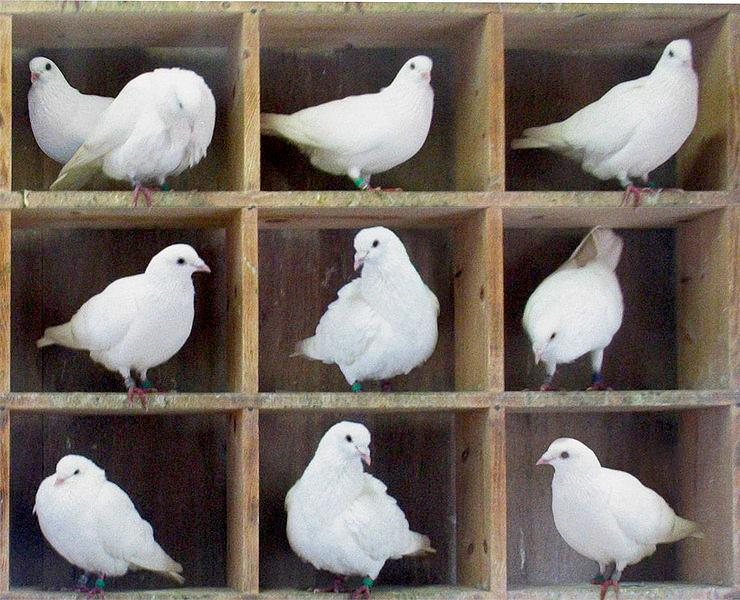
\includegraphics[width=\columnwidth,height=110pt]{pigeon.jpg}
\begin{center}
\vspace*{-7pt}
{\tiny Image source:\\
\url{http://en.wikipedia.org/wiki/File:TooManyPigeons.jpg}.\\[0.01pt]
\vspace*{-5pt}
Used under the license given there}
\end{center}
\end{column}
\end{columns}
The Pigeonhole Principle states that one pigeon will land in each
pigeonhole ($f$ is surjective) if and only if no two pigeons land in the same
location ($f$ is injective).
\end{spacing}
\newpage
\begin{spacing}{1}
The following theorem is another, equivalent formulation of the pigeonhole
principle. We will prove it first, and then show that it implies the
Pigeonhole Principle 2.4.20.\\[5pt]
\begin{THEOREM}
Let $M,N$ be finite sets and $f:M\to N$ surjective. Then $f$ is injective if and only if $\text{card}\,M=\text{card}\,N$.\\[6pt]
\end{THEOREM}
\begin{PROOF}
Suppose $M=\{a_1,\,...\,,a_m\}$, $\text{card}\,M=m$ and $\text{card}\,N=n$. Since $f$ is surjective, it follows that
\[n=\text{card}\,N=\text{card}\,\text{ran}\,f=\text{card}
\{f(a_1),\,...\,,f(a_m)\}\leq m\]
If $f$ is injective, then the numbers $f(a_1),\,...\,,f(a_m)$ are all distinct, and $\text{card}\{f(a_1),\,...\,,f(a_m)\}=m$. Thus, $m=n$.\\[5pt]
Suppose that $m=n$. Then $\text{card}\{f(a_1),\,...\,,f(a_m)\}=m$ so $f(a_1),\,...\,,f(a_m)$ are distinct. This implies that $f$ is injective.
\end{PROOF}
\end{spacing}
\newpage
\begin{spacing}{1.15}
\alert{Proof of the Pigeonhole Principle 2.4.20.}\\
Suppose that $M$ is finite and $f:M\to M$ is injective. Then $f:M\to\text{ran}\,f$ is surjective and injective. By Theorem 2.4.21, $\text{card}(\text{ran}\,f)=\text{card}\,M$. Since $\text{ran}\,f\subset M$, this implies (why?) that $\text{ran}\,f=M$. Thus $f:M\to M$ is surjective.\\[5pt]
Suppose that $f:M\to M$ is surjective. Then, by Theorem 2.4.21, $f$ is injective.\\[5pt]
Yet another version of the pigeonhole theorem is the following:\\[5pt]
\begin{THEOREM}
Let $M,N$ be finite sets with $\text{card}\,M>\text{card}\,N$ and $f:M\to N$. Then $f$ is not injective.\\[5pt]
\end{THEOREM}
The proof is left to the exercises.\\[5pt]
The pigeonhole principle seems almost trivial, but it is actually a very deep
theorem about the structure of finite sets. It does not hold true for infinite
sets, as the injective (but not surjective) map $f:\N\to\N,\,n\mapsto n+1$ shows.
\end{spacing}
\end{frame}
\begin{frame}[t,allowdisplaybreaks,allowframebreaks]{Applications of the Pigeonhole Principle}
\begin{spacing}{1.05}
The pigeonhole principle can be used to prove a wide variety of theorems,
some of which are quite surprising.\\[5pt]
\begin{LEMMA}
Let $n\in\N\setminus\{0\}$. Then there exists a multiple of $n$ such that its decimal expansion contains only the digits 1 and 0.\\[5pt]
\end{LEMMA}
\begin{PROOF}
Let $n\in\N\setminus\{0\}$ and consider the set of $n+1$ integers
\[M=\{1,~11,~111,\,...\,,\underbrace{11\,...\,1}_{n~\text{times}},
~\underbrace{11\,...\,11}_{n+1~\text{times}}\,\}.\]
Define the map $f:M\to\{0,\,...\,,n-1\},\,f(x)=x\,\text{mod}\,n$. By Theorem 2.4.22, $f$ is not injective, so there exist two elements in $M$ with the same remainder when divided by $n$. The larger of these less the smaller is an integer containing only 0s and 1s. Furthermore, it must have remainder 0 when divided by $n$, i.e., it is a multiple of $n$.
\end{PROOF}
\newpage
\begin{REMARK}
In many practical applications, the pigeon hole theorem
and related statements with respect to counting are formulated as
``putting $m$ objects into $k$ boxes.'' It should be obvious that this is
equivalent to finding a function from a set $M$ of $\text{card}\,M=m$ objects to a set $N$ of $\text{card}\,N=n$ boxes.\\[5pt]
Given arbitrary sets $X,Y$ and some map $f:X\to Y$ it is convenient to define the pre-image of a set $V\subset Y$ as
\[f^{-1}(V):=\{x\in X:f(x)\in V\}.\]
If $V$ contains only one element $V=\{v\}$, we often omit the braces, writing $f^{-1}(v)$ instead of $f^{-1}(\{v\})$. For example, defining the function $f:\R^2\to\R,f(x,y)=x^2+y^2$, the set
\[f^{-1}(r^2)=\{(x,y)\in\R^2:f(x,y)=r^2\}\]
is a circle of radius $r$ centered at the origin.
\end{REMARK}
\end{spacing}
\end{frame}
\begin{frame}[t]{The Generalized Pigeonhole Principle}
\begin{spacing}{1.05}
\stepcounter{zhuo}
\alert{2.4.25. Generalized Pigeonhole Principle.} Let $M,N$ be finite sets with cardinalities $\text{card}\,M=m$ and $\text{card}\,N=n$, respectively. Then for any function $f:M\to N$ there is at least one $n_0\in N$ such that $\text{card}(f^{-1}(n_0))\geq\lceil m/n\rceil$.\\[6pt]
\begin{PROOF}
We prove the theorem by contradiction. Suppose that for all $y\in\text{ran}\,f$
\[\text{card}(f^{-1}(y))<\lceil m/n\rceil.\]
Then also $\text{card}(f^{-1}(y))<m/n$, since $\text{card}(f^{-1}(y))\in\N$. Using $f^{-1}(y)\cap f^{-1}(y')=\emptyset$ for $y\neq y'$,
\[\text{card}\,M=\text{card}\bigg(\bigcup_{y\in\text{ran}\,f}f^{-1}(y)\bigg)=
\sum_{y\in\text{ran}\,f}\text{card}(f^{-1}(y))<n\frac{m}{n}=m,\]
which is a contradiction.
\end{PROOF}
\end{spacing}
\end{frame}
\begin{frame}[t]{Ramsey Theory}
\begin{spacing}{1.1}
We can apply the generalized pigeonhole theorem to a problem that occurs
in \emph{Ramsey theory}. In general, Ramsey theory is concerned with the
number of elements in a set such that a given property will hold. A
particular example is the following problem:\\[5pt]
\begin{EXAMPLE}
At a party consisting of 6 people, any two people are
either friends or enemies. Then there are either three mutual friends or
three mutual enemies at the party.\\[6pt]
Consider one member of the party, $A$. The five other members of the party
are either friends or enemies of $A$. By the generalized pigeonhole principle,
at least three of them are either friends or enemies of $A$. Suppose that
$B, C,D$ are friends of $A$. If any two of these three are friends, then they
together with $A$ are a group of three mutual friends. If none of $B, C,D$ are
friends, then they form a group of three mutual enemies.
If $B, C,D$ are a group of three enemies of $A$, the proof proceeds in a
similar manner.
\end{EXAMPLE}
\end{spacing}
\end{frame}
\begin{frame}[c,label=386]{Ramsey Numbers}
\begin{spacing}{1.1}
For $m,n\in\N\setminus\{0,1\}$ the \emph{Ramsey number $R(m,n)$} is defined as the
minimum number of people at a party so that there are either $m$ mutual
friends or $n$ mutual enemies. By Example 2.4.26,
\[R(3,3)\leq 6.\]
In the assignments you will prove $R(3,3)>5$, so $R(3,3)=6$.\\[6pt]
While a few interesting properties of Ramsey numbers are known, e.g., $R(m,n)=R(n,m)$ and $R(2,n)=n$, only a few Ramsey numbers are actually known. In fact, only nine Ramsey numbers with $3\leq m\leq n$ have been calculated! For example, $R(4,4)=18$. For other numbers, only bounds are known, e.g., $43\leq R(5,5)\leq 49$.
\end{spacing}
\end{frame}
\begin{frame}[t,allowdisplaybreaks,allowframebreaks]{Permutations}
\begin{spacing}{0.9}
\begin{DEFINITION}
Let $\{x_1,\,...\,,x_n\}$ be a set of  $n$ distinguishable elements $(x_k\neq x_j~\text{for}~j\neq k)$. Then an injective map
\[\pi:\{x_1,\,...\,,x_n\}\to\{x_1,\,...\,,x_n\}\]
is called a \emph{permutation} of these elements.\\[6pt]
By the pigeonhole principle, any permutation is automatically bijective.\\[5pt]
\end{DEFINITION}
\begin{REMARK}
A permutation is defined on a set of $n$ distinguishable elements; instead of $\{x_1,\,...\,,x_n\}$ we can also simply write $\{1,\,...\,,n\}$, replacing the permutation of elements with a permutation of indices.\\[6pt]
Recall that a function $f$ is defined as a set of pairs of the form $(x,f(x))$, where $x$ is the independent variable. Thus we could define a permutation $\pi$ through a set of pairs $\{(1,\pi(1)),\,...\,,(n,\pi(n))\}$. In fact, we do represent
permutations in this way, but use a different notation, writing
\[\pi=\begin{pmatrix}
        1 & 2 & ... & n \\
        \pi(1) & \pi(2) & ... & \pi(n)
      \end{pmatrix}\]
\end{REMARK}
\end{spacing}
\begin{spacing}{1.05}
\begin{EXAMPLE}
Consider the set of 3 objects, $\{1,2,3\}$. Then one permutation is given by the identity map,
\[\pi_0=\begin{pmatrix}
          1 & 2 & 3 \\
          1 & 2 & 3
        \end{pmatrix}\]
while other permutations are given by
\begin{equation*}
\begin{pmatrix}
          1 & 2 & 3 \\
          3 & 1 & 2
        \end{pmatrix},\qquad\begin{pmatrix}
          1 & 2 & 3 \\
          2 & 3 & 1
        \end{pmatrix},\qquad\begin{pmatrix}
          1 & 2 & 3 \\
          3 & 2 & 1
        \end{pmatrix},\qquad\begin{pmatrix}
          1 & 2 & 3 \\
          2 & 1 & 3
        \end{pmatrix},\qquad\begin{pmatrix}
          1 & 2 & 3 \\
          1 & 3 & 2
        \end{pmatrix}.
\end{equation*}
\begin{REMARK}
Instead of writing out the map as above, we often simply
give the ordered $n$-tuple $(\pi(1),\,...\,,\pi(n))$. For example, instead of
\begin{equation*}
  \begin{pmatrix}
    1 & 2 & 3 \\
    3 & 1 & 2
  \end{pmatrix}\qquad\qquad\quad\text{we might write}\qquad\qquad\quad
  (3,1,2).
\end{equation*}
\end{REMARK}
\end{EXAMPLE}
\!\!\begin{REMARK}
A permutation can be regarded as an arrangement of a
set; using the notation of Remark 2.4.30, the tuple $(3, 1, 2)$ can be
considered on the one hand as the values of a permutation; on the other
hand, it represents a specific ordering (or arrangement) of the elements of
the set $\{1, 2, 3\}$. In practice, the interpretation as an ordering is used in
applications.
\end{REMARK}
\newpage
\begin{LEMMA}
There are $n!$ permutations $\pi$ of the set $\{1,\,...\,,n\}$.\\[5pt]
\end{LEMMA}
\begin{PROOF}
We consider the number of possible values of $\pi(k),\,k=1,\,...\,,n$. The first value, $\pi(1)$ can be any of the $n$ elements of $\{1,\,...\,,n\}$. The second value can be any element of $\{1,\,...\,,n\}\setminus\{\pi(1)\}$. Hence there are $n$ possible values of $\pi(1)$, but only $n-1$ possible values of $\pi(2)$. In general, there are $n-k+1$ possible values for $\pi(k)$, so in total, there are
\[n\cdot(n-1)\cdots(n-n+1)=n!\]
different choices for the values $(\pi(1),\,...\,,\pi(n))$ of a permutation.
\end{PROOF}
\end{spacing}
\end{frame}
\begin{frame}[t,allowdisplaybreaks,allowframebreaks]{Permutations as Arrangements}
\begin{spacing}{1.05}
In combinatorics, permutations are regarded as \emph{arrangements in a definite order}. Clearly, the ordered tuple $(\pi(1),\,...\,,\pi(n))$ is an arrangement of $(1,\,...\,,n)$ is a definite order, i.e., the definition based on permutations
realizes this goal.\\[6pt]
Often one is interested in first selecting $r\leq n$ objects from $\{1,\,...\,,n\}$ and then arranging these objects in a definite order. We realize this by the
following, more general definition:\\[5pt]
\begin{DEFINITION}
Let $n,r\in\N\setminus\{0\}$ with $r\leq n$. Then an injective map
\[\pi:\{1,\,...\,,r\}\to\{1,\,...\,,n\}\]
is called an \emph{r-permutation} of $r$ elements from $\{1,\,...\,,n\}$.
\end{DEFINITION}
\newpage
\stepcounter{zhuo}
\alert{2.4.34. Notation.} We again write $\pi$ as
\begin{equation*}
  \begin{pmatrix}
    1 & 2 & ... & r \\
    \pi(1) & \pi(2) & ... & \pi(r)
  \end{pmatrix}\qquad\quad\text{or}\quad\qquad
  (\pi(1),\,...\,,\pi(r)),
\end{equation*}
where $\pi(k)\in\{1,\,...\,,n\},\,k=1,\,...\,,r$.\\[5pt]
\begin{EXAMPLE}
Let $n=3,r=2$. Then the following are permutations of two elements from $\{1,2,3\}$:
\[(1,2),\qquad\quad(2,1),\qquad\quad
(1,3),\qquad\quad(3,1),\qquad\quad
(2,3),\qquad\quad(3,2).\]
\end{EXAMPLE}
\begin{THEOREM}
There are
\[n\cdot(n-1)\cdots(n-r+1)=\frac{n!}{(n-r)!}\]
different permutations of $r$ elements from $\{1,\,...\,,n\}$.
\end{THEOREM}
\end{spacing}
\end{frame}
\begin{frame}[t,allowdisplaybreaks,allowframebreaks]{Combinations}
\begin{spacing}{1.1}
A related question arising in combinatorics is the number of selections of $r$
elements from a set of $n$ elements, where we do not care about the order.
Such selections are called $r$ -combinations.\\[5pt]
\begin{EXAMPLE}
Let $n=3,r=2$. Then the following are combinations of two elements from $\{1,2,3\}$:
\[\{1,2\},\qquad\qquad\qquad\{1,3\},\qquad
\qquad\qquad\{2,3\}.\]
Note that a selection consists of sets (which are unordered) while a
permutation consists of ordered tuples.\\[5pt]
\begin{DEFINITION}
A combination of $r$ elements from $\{1,\,...\,,n\}$ is subset $A\subset\{1,\,...\,,n\}$ with $\text{card}\,A=r$ elements.
\end{DEFINITION}
\end{EXAMPLE}
\end{spacing}
\newpage
\begin{spacing}{0.9}
\begin{THEOREM}
There are
\[\binom{n}{r}=\frac{n!}{r!(n-r)!}\]
combinations of $r$ elements from $\{1,\,...\,,n\}$.\\[5pt]
\end{THEOREM}
\begin{PROOF}
We first consider permutations of $r$ objects from $\{1,\,...\,,n\}$. Every permutation gives us a combination, by identifying
\[(\pi(1),\,...\,,\pi(r))\longrightarrow\{\pi(1),\,...\,,\pi(r)\}.\]
Obviously, more than one permutation will give us the same combination.
Note that any permutation of $(\pi(1),\,...\,,\pi(r))$ will be a permutation of $r$ objects from $\{1,\,...\,,n\}$. Furthermore, any permutation of $(\pi(1),\,...\,,\pi(r))$ will yield the same combination. For each tuple $(\pi(1),\,...\,,\pi(r))$, there are $r!$ permutations of $(\pi(1),\,...\,,\pi(r))$, so we need to divide the total number of permutations of $r$ objects from $\{1,\,...\,,n\}$ by $r!$.
\end{PROOF}
\end{spacing}
\end{frame}
\begin{frame}[c]{Combinations as Permutations of Indistinguishable Objects}
\begin{spacing}{1.2}
A combination of $r$ elements of $\{1,\,...\,,n\}$ is similar to a permutation, but
without regard to order. Fundamentally, if we do not order the selected
objects, we regard them as indistinguishable once they have been selected.
(We can not say ``Take the fifth selected object,'' but merely, ``Take a
selected object.'' We do not distinguish between the selected objects.)\\[6pt]
Therefore, a combination can be regarded as \emph{a permutation of r indistinguishable objects from $\{1,\,...\,,n\}$}.\\[5pt]
Effectively, this corresponds to a division of $\{1,\,...\,,n\}$ into two classes, a subset consisting of $r$ elements and its complement.
\end{spacing}
\end{frame}
\begin{frame}[t,allowdisplaybreaks,allowframebreaks]{Sorting Into Classes}
\begin{spacing}{1.15}
We can hence reformulate Theorem 2.4.39 on combinations with regard to the problem of sorting elements of $\{1,\,...\,,n\}$ into two classes (sets) $A_1$ and $A_2$ of specified size.\\[6pt]
\begin{THEOREM}
Let $\mathcal{N}:=\{1,\,...\,,n\}$. Then there are
\[\frac{\text{card}\,\mathcal{N}!}{\text{card}\,A_1!\,\text{card}\,A_2!}
=\frac{n!}{n_1!n_2!}=\frac{n!}{r!(n-r)!}=\binom{n}{r}\]
possible ways of dividing $\mathcal{N}$ into two sets $A_1$ and $A_2$, where
\begin{itemize}
  \item $A_1\subset\mathcal{N},\,\text{card}\,A_1=n_1=r$,
  \item $A_2=\mathcal{N}\setminus A_1,\,\text{card}\,A_2=n_2=n-r$.
\end{itemize}
\vspace*{6pt}
Of course, this result can be generalized!
\end{THEOREM}
\newpage
\begin{THEOREM}
Let $\mathcal{N}:=\{1,\,...\,,n\}$. Then there are
\[\frac{n!}{n_1!n_2!...n_k!}\]
possible ways of dividing $\mathcal{N}$ into $k$ sets $A_1,\,...\,,A_k$, where
\begin{itemize}
  \item $\mathcal{N}=\bigcup_{i=1}^kA_i,\qquad A_i\cap A_j=\emptyset$ for $i\neq j$,
  \item $\text{card}\,A_i=n_i,\,i=1,\,...\,,k$.
\end{itemize}
\vspace*{8pt}
\begin{REMARK}
Since we are only interested in dividing a number of
elements into classes, and do not distinguish between the elements within
each class, this sorting into classes is also called \emph{permutation of
indistinguishable objects}.
\end{REMARK}
\end{THEOREM}
\end{spacing}
\newpage
\begin{spacing}{1}
\alert{Proof of Theorem 2.4.41.}\\
We first count the number of ways of sorting $n_1$ elements into $A_1$:
\[\binom{n}{n_1}=\frac{n!}{n_1!(n-n_1)!}.\]
Next we count the ways of sorting $n_2$ elements of the remaining $n-n_1$ elements into $A_2$:
\[\binom{n-n_1}{n_2}=\frac{(n-n_1)!}{n_2!(n-n_1-n_2)!}.\]
The total number of ways of sorting $n_1$ elements into $A_1$ and $n_2$ elements into $A_2$ is then the product
\[\binom{n}{n_1}\binom{n-n_1}{n_2}=\frac{n!}{n_1!(n-n_1)!}\frac{(n-n_1)!}{n_2!(n-n_1-n_2)!}
=\frac{n!}{n_1!n_2!(n-n_1-n_2)!}\]
\newpage
\alert{Proof of Theorem 2.4.41 (continued).}\\
Proceeding in this manner, we find there are
\begin{equation*}
  \begin{split}
     \binom{n}{n_1}\prod\limits_{i=1}^{k-1}\binom{n-\sum\nolimits_{j=1}^{i}n_j}{n_{i+1}} &=\frac{n!}{n_1!(n-n_1)!}\prod\limits_{i=1}^{k-1}\frac{(n-\sum\nolimits_{j=1}^{i}n_j)!}{n_{i+1}!(n-\sum\nolimits_{j=1}^{i+1}n_j)!} \\
       &=\frac{n!}{n_1!(n-n_1)!}\frac{\prod\nolimits_{i=1}^{k-1}(n-\sum\nolimits_{j=1}^{i}n_j)!}{\prod\nolimits_{i=1}^{k-1}n_{i+1}!\prod\nolimits_{i=1}^{k-1}(n-\sum_{j=1}^{i+1}n_j)!} \\
       &=\frac{n!}{\prod\nolimits_{i=1}^{k}n_i!}\frac{\prod\nolimits_{i=2}^{k-1}(n-\sum\nolimits_{j=1}^{i}n_j)!}{\prod\nolimits_{i=1}^{k-2}(n-\sum\nolimits_{j=1}^{i+1}n_j)!} \\
       &=\frac{n!}{\prod\nolimits_{i=1}^{k}n_i!}
  \end{split}
\end{equation*}
ways of sorting all objects into classes $A_1,\,...\,,A_k,\,\text{card}\,A_i=n_i$.
\hfill$\square$
\end{spacing}
\end{frame}
\begin{frame}[t]{Repetition}
\begin{spacing}{1.1}
Recall that $r$-permutations are arrangements of $r$ objects from a set of $n\geq r$ objects, represented through $r$-tuples. Similarly, $r$-combinations are selections of $r$ objects but without regard to order, hence represented as sets of cardinality $r$. These two problems have one thing in common, which we only mentioned in passing: the $r$ selected/arranged objects are all \emph{distinct}.\\[5pt]
What happens if we drop this requirement, i.e., we allow identical objects
to appear in our selections/arrangements? This is known as
selection/arrangement \emph{with repetition}.\\[6pt]
In the case of arrangements with repetition, this is quite easy: in an
$r$-tuple, we now allow any entry to contain an arbitrary element of our set $\{1,\,...\,,n\}$, regardless of what is contained in the other entries. Thus, the set of all $r$-\emph{permutations with repetition} is just $\{1,\,...\,,n\}^r$ and has cardinality $n^r$ by Theorem 2.4.10. There are $n^r$ different $r$-permutations with repetition.
\end{spacing}
\end{frame}
\begin{frame}[t]{Repetition and Multisets}
\begin{spacing}{1}
Dealing with combinations with repetition is a bit more subtle: A
2-combination is, for example, the set $\{a,b\}$, but a 3-combination with repetition might be $\{a,b,b\}=\{a,b\}$. So the ``information'' that the element $b$ is to be repeated (or selected twice) is lost if we just use set formalism.\\[6pt]
A solution is to introduce \emph{multisets}. These are unordered collections of
objects (like sets) but also associate to each object a so-called \emph{multiplicity}.
For example, the set
\[\{2a,4b,c\}\]
contains the elements $a, b, c$ with multiplicities 2, 4, 1, respectively. The
multiplicities are generally integers and keep track of ``how many times'' an
element is included in the set. Multisets are related to fuzzy sets (that you
encountered in the exercises) and follow a similar calculus. We will define
the cardinality of a multiset as the sum of the multiplicities of its elements.
Then an $r$-\emph{combinations with repetition} is simply a multiset of cardinality
$r$, or an $r$-multiset.
\end{spacing}
\end{frame}
\begin{frame}[c]{Combinations and Permutations with Repetition}
\begin{spacing}{1.05}
Note that in allowing $r$-permutations and $r$-combinations of $n$ elements
with repetition, we no longer require $r\leq n$.\\[5pt]
\begin{EXAMPLE}
Consider the set $S=\{a,b,c\}$. Then
\[(b,a,b,c,a,b,b)\]
is a 7-permutation with repetition of $S$. The 7-multiset
\[\{2a,4b,c\}\]
represents the corresponding 7-combination of $S$.\\[5pt]
We have already discussed that there are $n^r=3^7=2187$ possible 7-permutations with repetition. But how many different 7-combinations are there?
\end{EXAMPLE}
\end{spacing}
\end{frame}
\begin{frame}[t,allowdisplaybreaks,allowframebreaks]{Counting Multisets}
\begin{spacing}{1.05}
Let us stay with the special case of Example 2.4.43. It is clear that the
number of possible 7-combinations is equal to the number of multisets of
cardinality 7. Suppose that we write
\[\{2a,4b,c\}=\{a,a,b,b,b,b,c\}.\]
Now if we agree to always list the elements of a multiset containing elements of $S=\{a,b,c\}$ in a definite order, we need only write
\[x,x,\mid,x,x,x,x,\mid,x\]
to indicate the set $\{2a,4b,c\}$. By our convention, the first $x$s will stand for $a$s until a bar $\mid$ is reached, then the $x$s will stand for $b$s etc. We can also leave out the commas. Thus,
\[|xxx|xxxx\qquad\qquad\quad\text{stands for the 7-multiset}\qquad\qquad\quad
\{3b,4c\}.\]
\newpage
We see that the multisets are determined entirely by the position of the
bars among the $x$s. In our example, we need 2 bars to indicate the
separation between $a, b, c$ and have 7 $x$s to indicate the elements of the
7-multiset. We can regard this as follows: we have 9 ``slots'' and each slot
is either filled by a bar or an $x$. Since the $x$s by themselves can be any
element of $S=\{a,b,c\}$, the number of multisets is determined by number of ways to select the two slots that hold the bars. In our example, there are $\binom{9}{2}=36$ ways to select these slots.\\[6pt]
This argument immediately generalizes to yield the following theorem:\\[5pt]
\begin{THEOREM}
For $r,n\in\N\setminus\{0\}$ here are
\[\binom{r+n-1}{n-1}=\binom{r+n-1}{r}\]
$r$-combinations of $n$ elements with repetition. (Or that many $r$-multisets of $n$ elements.)
\end{THEOREM}
\newpage
\vspace*{10pt}
\begin{EXAMPLE}
Consider the equation
\[x_1+x_2+x_3=11,\qquad\qquad\qquad
x_1,x_2,x_3\in\N.\]
We are interested in finding the number of solutions to this equation.
Note that this equation is equivalent to the following: select a total of 11
items, where $x_1$ items are of type 1, $x_2$ are of type 2 and $x_3$ are of type 3. Thus, each solution corresponds to an 11-multiset of 3 three elements and there are
\[\binom{11+3-1}{11}=78\]
different solutions.
\end{EXAMPLE}
\end{spacing}
\end{frame}
\begin{frame}[t,allowdisplaybreaks,allowframebreaks]{The Inclusion-Exclusion Principle}
\begin{spacing}{0.85}
In Theorem 2.4.16 we have proven that for two finite sets $A,B$,
\begin{equation}\label{2.4.3}
\text{card}(A\cup B)=\text{card}\,A+\text{card}\,B-\text{card}(A\cap B).
\end{equation}
For the following arguments we will write $|A|$ for $\text{card}\,A$ for brevity. It turns out that \eqref{2.4.3} can be generalized; for instance,
\begin{equation*}
  \begin{split}
     |A\cup B\cup C| &=|A|+|B|+|C|-|A\cap B|-|B\cap C|-|A\cap C| \\
       &+|A\cap B\cap C|.
  \end{split}
\end{equation*}
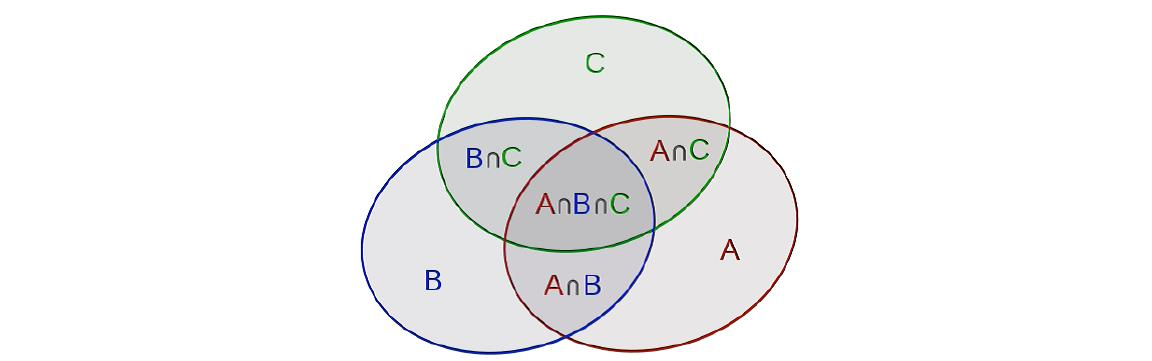
\includegraphics[width=\textwidth,height=80pt]{ie.jpg}\\
{\tiny \qquad\qquad\qquad\qquad
Image source:\url{http://commons.wikimedia.org/wiki/File:Inclusion-exclusion.svg} \quad Used under the license given there}
\end{spacing}
\newpage
\begin{spacing}{1.1}
\vspace*{9pt}
The general theorem which governs the cardinality of the union of $n$ sets is
called the \emph{Inclusion-Exclusion Principle}\\[6pt]
\stepcounter{zhuo}
\alert{2.4.46. Inclusion-Exclusion Principle.} For any sets $A_1,\,...\,,A_n,\,n\in\N$,
\begin{equation}\label{2.4.4}
 \begin{split}
    |A_1\cup A_2\cup...\cup A_n|= &\sum_{1\leq i\leq n}|A_i|-\sum_{1\leq i<j\leq n}|A_i\cap A_j| \\
      &+\sum_{1\leq i<j<k\leq n}|A_i\cap A_j\cap A_k| \\
      &-+\,...+(-1)^{n+1}|A_1\cap A_2\cap...\cap A_n|
 \end{split}
\end{equation}
\newpage
\begin{PROOF}
We will show that the right-hand side of \eqref{2.4.4} counts every element of the union $\bigcup A_i$ exactly once. Suppose that an element $a$ is contained in exactly $r$ of the sets $A_1\,...\,,A_n,\,1\leq r\leq n$. Then the first sum counts $a$ exactly $r=\binom{r}{1}$ times. The second sum counts $a$ $\binom{r}{2}$ times, since there are $\binom{r}{2}$ pairs of sets which both contain $a$. In general, a sum involving the  intersection of $m$ sets will count $a$ $\binom{r}{m}$ times.\\[7pt]
Therefore, the number of times that the right-hand side \eqref{2.4.4} counts $a$ is
\begin{equation*}
  \begin{split}
     \binom{r}{1}-\binom{r}{2}+-\cdots+(-1)^{r+1}\binom{r}{r} &=1-\sum_{m=0}^{r}(-1)^m\binom{r}{m} \\
       &=1-(1-1)^r=1
  \end{split}
\end{equation*}
\end{PROOF}
\end{spacing}
\end{frame}
\begin{frame}[t]{Inclusion-Exclusion (Alternative Form)}
\begin{spacing}{1.05}
Suppose that $S$ is a finite set and $A_1,\,...\,,A_n\subset S$. Then
\[A_1\cap A_2\cap\cdots\cap A_n=S\setminus(A_1^c\cup A_2^c\cup\cdots\cup A_n^c)\]
and, therefore,
\begin{align}\label{2.4.5}
  |A_1\cap A_2\cap...\cap A_n| &=|S|-|A_1^c\cup A_2^c\cup...\cup A_n^c|\nonumber \\
   &=|S|-\sum_{1\leq i\leq n}|A_i^c|+\sum_{1\leq i<j\leq n}|A_i^c\cap A_j^c|\nonumber \\
   &-+\,...+(-1)^n|A_1^c\cap A_2^c\cap...\cap A_n^c|.
\end{align}
We can apply \eqref{2.4.5} to certain counting problems.\\[6pt]
\begin{EXAMPLE}
We are interested in the number of primes less than or equal to $n$ for a given $n\in\N\setminus\{0,1\}$. By Theorem 1.7.7, to check whether a number $p$ is prime, it suffices to check whether it is a multiple of any number less than $\sqrt{p}$.
\end{EXAMPLE}
\end{spacing}
\end{frame}
\begin{frame}[t,allowdisplaybreaks,allowframebreaks]{Counting Prime Numbers}
\begin{spacing}{1.05}
Suppose we are interested in the number of primes less than $n = 120$.
Then we need to eliminate from $S=\{2,3,\,...\,,120\}$ all composite numbers, i.e., all numbers with prime factors less than $\lfloor\sqrt{120}\rfloor=10$. These are the numbers $2,3,5,7$, so let
\begin{align*}
  A_1 &:=\{q\in S:2\mid q\}, & A_2 &:=\{q\in S:3\mid q\}, \\
  A_3 &:=\{q\in S:5\mid q\}, & A_4 &:=\{q\in S:7\mid q\}.
\end{align*}
Then a prime number in $S$ will be equal to $2,\:3,\:5$ or 7 or an element of $A_1^c\cap A_2^c\cap A_3^c\cap A_4^c$. We apply \eqref{2.4.5}:
\begin{equation}\label{2.4.6}
  \begin{split}
     |A_1^c\cap A_2^c\cap A_3^c\cap A_4^c| &=|S|-\sum_{i=1}^{4}|A_i|+\sum_{1\leq i<j\leq 4}|A_i\cap A_j| \\
       &-\sum_{1\leq i<j<k\leq 4}|A_i\cap A_j\cap A_k|+|A_1\cap A_2\cap A_3\cap A_4|
  \end{split}
\end{equation}
\end{spacing}
\newpage
\begin{spacing}{1}
We use that
\[|\{q\in S:n\mid q\}|=120\,\text{div}\,n=\lfloor 120/n\rfloor\]
Then
\[|S|=119,\qquad |A_1|=60,\qquad |A_2|=40,\qquad |A_3|=24,\qquad
|A_4|=17.\]
Furthermore,
\begin{align*}
  A_1\cap A_2 &=\{q\in S:6\mid q\}, & |A_1\cap A_2| &=20, \\
  A_1\cap A_3 &=\{q\in S:10\mid q\}, & |A_1\cap A_3| &=12, \\
  A_1\cap A_4 &=\{q\in S:14\mid q\}, & |A_1\cap A_4| &=8, \\
  A_2\cap A_3 &=\{q\in S:15\mid q\}, & |A_2\cap A_3| &=8, \\
  A_2\cap A_4 &=\{q\in S:21\mid q\}, & |A_2\cap A_4| &=5, \\
  A_3\cap A_4 &=\{q\in S:35\mid q\}, & |A_3\cap A_4| &=3,
\end{align*}
\end{spacing}
\newpage
\begin{spacing}{0.8}
\begin{align*}
  A_1\cap A_2\cap A_3 &=\{q\in S:30\mid q\}, & |A_1\cap A_2\cap A_3| &=4,\\
  A_1\cap A_2\cap A_4 &=\{q\in S:42\mid q\}, & |A_1\cap A_2\cap A_4| &=2,\\
  A_1\cap A_3\cap A_4 &=\{q\in S:70\mid q\}, & |A_1\cap A_3\cap A_4| &=1,\\
  A_2\cap A_3\cap A_4 &=\{q\in S:105\mid q\}, & |A_2\cap A_3\cap A_4| &=1
\end{align*}
and finally,
\[A_1\cap A_2\cap A_3\cap A_4=\{q\in S:210\mid q\},\qquad |A_1\cap A_2\cap A_3\cap A_4|=0.\]
Inserting these values into \eqref{2.4.6}, we obtain
\begin{equation*}
  \begin{split}
     |A_1^c\cap A_2^c\cap A_3^c\cap A_4^c|= &\,119-60-40-24-17 \\
       &+20+12+8+8+5+3-4-2-1-1+0 \\
       =&\,26
  \end{split}
\end{equation*}
Hence, there are $4+26=30$ primes less than or equal to 120. We have found\\[3pt] these primes through the Sieve of Eratosthenes in Example 1.7.9.
\end{spacing}
\end{frame}
\begin{frame}[c]{The Prime Number Theorem}
\begin{spacing}{1.1}
More generally, the number of prime numbers less than a given $n$ is of
significant interest. The following result is quite difficult to prove and we
only state it here for reference:\\[6pt]
\stepcounter{zhuo}
\alert{2.4.48. Prime Number Theorem.} Let $\pi(n)$ denote the number of prime numbers less than or equal to $n\in\N$. Then
\[\lim_{n\to\infty}\frac{\pi(n)}{n/\ln(n)}=1,\]
where $\ln$ denotes the natural logarithm (to base $e=2.71828\,...$).
\end{spacing}
\end{frame}
\subsection{Probabilistic Algorithms}
\begin{frame}[c] \begin{spacing}{2.5}
\tableofcontents[sectionstyle=hide,subsectionstyle=show/shaded/hide] \end{spacing}
\end{frame}
\begin{frame}[t,allowdisplaybreaks,allowframebreaks]{Classical Definition of Probability}
\begin{spacing}{0.9}
In this section we will introduce some methods based on the simple,
classical concept of probability.\\[5pt]
\setcounter{equation}{0}
\begin{DEFINITION}
Let $A$ be a random outcome of an experiment that may
proceed in various ways. Assume each of these ways is equally likely. Then
the probability of the outcome $A$, denoted $P[A]$, is
\[P[A]=\frac{\text{number of ways leading to outcome }A}{\text{number of ways the experiment can proceed.}}\]
\begin{EXAMPLES}
\begin{itemize}
  \item[(i)] The experiment consists of flipping a coin. We are interested in the probability of the coin landing heads up. The experiment can proceed in two ways: the coin land heads up or tails up. We assume each event is equally likely, so the classical definition gives
      \[P[\text{coin lands heads up}]=\frac{1}{2}=0.5\]
\newpage
  \item[(ii)] The experiment consists of rolling two 6-sided dice and summing the results, so the possible outcomes are the numbers $S=2,3,\,...\,,12$. We are interested in the outcome $S=3$. Each die will give results $1,2,3,4,5$ or 6. We assume that each result is equally likely. There are two ways we can get the outcome $S = 3$: either the first die's result is 1 and the second die's result is 2, or the first die gives 2 and the second die gives 1. In total, the experiment can proceed in $6\times 6=36$ different ways. Hence
      \[P[3]=\frac{2}{36}=\frac{1}{18}=0.056\]
\end{itemize}
\end{EXAMPLES}
\end{DEFINITION}
\end{spacing}
\end{frame}
\begin{frame}[t]{Sample Spaces and Sample Points}
\begin{spacing}{1.1}
The techniques of counting permutations, combinations and sorting into
classes are very useful for evaluating probabilities by the classical
definition. First, however, we need to translate physical situations into a
mathematical context.\\[5pt]
\begin{DEFINITION}
A \emph{sample space} for an experiment is a set $S$ such that
each physical outcome of the experiment corresponds to exactly one
element of $S$.\\[5pt]
An element of $S$ is called a sample point.\\[6pt]
\end{DEFINITION}
\begin{REMARK}
Not every element of a sample space needs to correspond
to the outcome of an experiment. It is often convenient to select a very
large, but simple sample space. For example, for the roll of a six-sided die,
we can take $S = \N$, where the result of the die corresponds to the natural
numbers 1,2,3,4,5 or 6 and all other natural numbers are not used. All
natural numbers in this example are sample points, even though only six
actually correspond to physical reality.
\end{REMARK}
\end{spacing}
\end{frame}
\begin{frame}[t]{Events}
\begin{spacing}{1.1}
\begin{DEFINITION}
Any subset $A$ of a sample space $S$ is called an \emph{event}.\\[6pt]
\end{DEFINITION}
\begin{EXAMPLE}
We roll a four-sided die 10 times. Then a possible sample space is $S=\N^{10}$ and a sample point is a 10-tuple, for example $(1,2,3,2,3,3,1,1,4,4)\in\N^{10}$.
\begin{columns}[onlytextwidth]
\begin{column}{0.7\textwidth}
This sample point corresponds to first rolling a one, then a 2, next a 3, followed by a 2, a 3, a 3, two ones and two fours.\\[6pt]
An event might correspond to ``rolling at least two fours'' in which case this would be a sub\-set $A\subset S$ such that each 10-tuple in $A$ has at least  two entries equal to 4. For example $(1,2,3,2,3,3,1,1,4,4)\in A$ but $(1,2,3,2,3,3,1,1,3,4)\notin A$.
\end{column}
\begin{column}{0.3\textwidth}
\begin{spacing}{0.5}
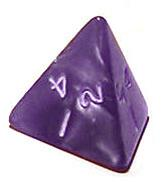
\includegraphics[width=\columnwidth]{die.jpg}\\
\begin{tiny}
  Image source:\\
\url{http://commons.wikimedia.org/wiki/
File:4-sided_dice_250.jpg}.\\
Used under the license given there
\end{tiny}
\end{spacing}
\end{column}
\end{columns}
\end{EXAMPLE}
\end{spacing}
\end{frame}
\begin{frame}[t]{Example}
\begin{spacing}{1.05}
\begin{EXAMPLE}
We roll a four-sided die 10 times. What is the probability of obtaining 5 ones, 3 twos, 1 three and 1 four?\\[6pt]
There are $4^{10}=1048576$ possibilities for the 10-tuple of results of the die rolls, corresponding to that many sample points in $S=\N^{10}$ that correspond to physical results. The event $A$ consists of all ordered 10-tuples containing 5 ones, 3 twos, 1 three and 1 four. There are
\[\frac{10!}{5!3!1!1!}=5040\]
possible ways of obtaining 5 ones, 3 twos, 1 three and 1 four, so there are that many elements in $A$. The probability is
\[\frac{5040}{1048576}\approx 0.00481\approx 0.5\%.\]
\end{EXAMPLE}
\end{spacing}
\end{frame}
\begin{frame}[t]{Properties of Events}
\begin{spacing}{1.1}
We can interpret events as follows: Suppose $S$ is a sample space and $A_1,A_2\subset S$.
\begin{enumerate}[(i)]
  \item The event $A_1\cap A_2$ contains all sample points corresponding to outcomes common to $A_1$ and $A_2$.\\[5pt]
      $A_1,A_2$ are said to be \emph{mutually exclusive} if $A_1\cap A_2=\emptyset$.
  \item The event $A_1\cup A_2$ contains all sample points corresponding to outcomes in either $A_1$ or $A_2$.
\end{enumerate}
If our sample space $S$ contains a finite number of sample points (i.e., $\text{card}\,S<\infty$) and $P[A_1]$ and $P[A_2]$ are given, we can calculate $P[A_1\cap A_2]$ and $P[A_1\cup A_2]$.\\[6pt]
However, some sample spaces are countably or even uncountably infinite in
size. It is then easier to simply define the properties that a ``probability'' is
supposed to have in such a way that the definition coincides with the
results obtained by counting whenever $S$ is finite.
\end{spacing}
\end{frame}
\begin{frame}[t]{Definition of Probability}
\begin{spacing}{1.05}
\begin{DEFINITION}
Let $S$ be a sample space and $\mathcal{P}(S)$ the power set of $S$. Then a function
\[P:\mathcal{P}(S)\to\R,\qquad\qquad\qquad
A\mapsto P[A]\]
is called a \emph{probability function} (or just \emph{probability}) on $S$ if
\begin{enumerate}[(i)]
  \item $P[A]\geq0$ for all $A\subset S$,
  \item $P[S]=1$,
  \item For any set of events $\{A_k\}\subset\mathcal{P}(A)$ such that $A_i\cap A_k=\emptyset$ for $i\neq k$,
      \[P\left[\bigcup A_k\right]=\sum P[A_k].\]
      This equation holds also if $\{A_k\}$ is an infinite set of $A_k$, in which case the union and the sum are also infinite.
\end{enumerate}
\end{DEFINITION}
\end{spacing}
\end{frame}
\begin{frame}[t,allowdisplaybreaks,allowframebreaks]{Probabilities of Events}
\begin{spacing}{0.9}
A subset $A\in\mathcal{P}(S)$ is an event in sample space. We therefore interpret events as follows:
\begin{itemize}
  \item $A=\emptyset$ is the event that ``nothing happens'' (an experiment has no outcome found in $S$)
  \item $A=S$ is the event that ``something happens'' (the experiment has some outcome in $S$)
  \item $A^c=S\setminus A$ represents all outcomes that do not include those associated to $A$
\end{itemize}
By Definition 2.5.8,
\[P[S]=1,\qquad\qquad P[\emptyset]=0,\qquad\qquad
P[A^c]=1-P[A],\]
where the first equation is given by definition and the latter two follow
easily from the properties of the probability function.\\[5pt]
It is also not difficult to show that
\setcounter{equation}{0}
\begin{equation}\label{2.5.1}
P[A_1\cup A_2]=P[A_1]+P[A_2]-P[A_1\cap A_2],\qquad\quad A_1,A_2\in\mathcal{P}(S).
\end{equation}
\end{spacing}
\newpage
\begin{spacing}{1.1}
Note that \eqref{2.5.1} implies \emph{Boole's inequality},
\begin{equation}\label{2.5.2}
P[A_1\cup A_2]\leq P[A_1]+P[A_2],
\end{equation}
for all $A_1,A_2\in\mathcal{P}(S)$.\\[5pt]
Another easy property is that if $A_1\subset A_2$, then $P[A_1]\leq P[A_2]$.\\[5pt]
\begin{EXAMPLE}
Suppose that two four-sided dice are rolled. We take the sample space
\[S=\{(1,1),(1,2),(1,3),(1,4),(2,1),\,...\,,(4,3),(4,4)\},\]
where each tuple has the form (1\textsuperscript{st} result, 2\textsuperscript{nd} result). We then assign the probability function $P[\{(i,j)\}]=1/16$ for $i,j=1,2,3,4$. By defining the probability for each one-element subset of $S$ we are fixing the probability for any event $A\subset S$. Our definition has been chosen to coincide with the
probability of obtaining each sample point according to Definition 2.5.1 if
the dice are fair.
\end{EXAMPLE}
\end{spacing}
\newpage
\begin{spacing}{0.5}
Let $A_1$ be the event that corresponds to the outcome ``the sum of the two die rolls is at most 3'' and $A_2$ correspond to the outcome ``the two die rolls give the same number''. Then
\[A_1=\{(1,1),(1,2),(2,2)\},\qquad\quad
A_2=\{(1,1),(2,2),(3,3),(4,4)\}.\]
The probability of these events is calculated as
\begin{align*}
  P[A_1] &=P[\{(1,1)\}]+P[\{(1,2)\}]+P[\{(2,1)\}]=\frac{3}{16}, \\
  P[A_2] &=\frac{4}{16}=\frac{1}{4}.
\end{align*}
Then we can calculate for example that the probability of ``the sum of two
die rolls is at most three and both rolls are the same'' is
\[P[A_1\cap A_2]=P[\{1,1\}]=\frac{1}{16},\]
the probability of ``the two die rolls are distinct'' is
\[P[A_2^c]=1-P[A_2]=\frac{3}{4}.\]
\end{spacing}
\end{frame}
\begin{frame}[t]{The Probabilistic Inclusion-Exclusion Principle}
\begin{spacing}{1.05}
We note that the generalization of \eqref{2.5.1} is given by the inclusion-exclusion principle,\\[6pt]
\stepcounter{zhuo}
\alert{2.5.10. Inclusion-Exclusion Principle.} Let $S$ be a sample space and $A_1,\,...\,,A_n\subset S$. Then
\begin{equation}\label{2.5.3}
\begin{split}
P[A_1\cup A_2\cup\cdots\cup A_n]=&\sum_{1\leq i\leq n}P(A_i)-\sum_{1\leq i<j\leq n}P[A_i\cap A_j]\\
     &+\sum_{1\leq i<j<k\leq n}P[A_i\cap A_j\cap A_k] \\
     &-+\,...+(-1)^{n+1}P[A_1\cap A_2\cap\cdots\cap A_n]
\end{split}
\end{equation}
Since $S$ need not be a countable set, this version of the theorem is best
proven using induction in $n$. We omit the proof here.
\end{spacing}
\end{frame}
\begin{frame}[t,allowdisplaybreaks,allowframebreaks]{Conditional Probability}
\begin{spacing}{1.1}
\vspace*{-6pt}
We have seen from this example how the relations derived from the axioms
of Definition 2.5.8 allow us to calculate the probability that
\begin{itemize}
  \item ``event $A$ occurs'',
  \item ``event $A$ does not occur'',
  \item ``events $A$ and $B$ occur'' and
  \item ``event $A$ or event $B$ occurs''.
\end{itemize}
The axioms do not, however, provide us with a way to calculate the
probability that ``event $B$ occurs if event $A$ has occurred.'' For this, we
need to make an additional definition, which we now introduce.\\[5pt]
Let us denote by $P[B\mid A]$ the probability that ``$B$ occurs given that $A$ has occurred''. Let us use Example 2.5.9 for illustration. Suppose we are interested in $P[A_1\mid A_2]$, i.e., the probability that the sum of the die rolls is
less than four given that the rolls are equal. Effectively, 4 out of 16
outcomes lead to event $A_2$, and only one out these 4 gives rise to an element in $A_1\cap A_2=\{(1,1)\}$.
\newpage
If we count the number of sample points (``outcomes'') in $A_2$ that give $A_1\cap A_2$ to obtain the probability of obtaining $A_1$ given that $A_2$ has occurred, we essentially have
\[P[A_1\mid A_2]=\frac{\text{card}(A_1\cap A_2)}{\text{card}\,A_2}=\frac{P[A_1\cap A_2]}{P[A_2]}.\]
This motivates the following definition:\\[5pt]
\begin{DEFINITION}
Let $A,B\subset S$ be events and $P[A]\neq 0$. Then
\[P[B\mid A]:=\frac{P[A\cap B]}{P[A]}.\]
is said to be the \emph{conditional probability} of $B$ given $A$.
\end{DEFINITION}
\end{spacing}
\end{frame}
\begin{frame}[c]{Independence of Events}
\begin{spacing}{1.1}
If one event does not influence another, then we say that the two events
are \emph{independent}. Mathematically, we express this in the following way.\\[6pt]
\begin{DEFINITION}
Let $A,B$ be two events. We say that $A$ and $B$ are independent if
\begin{equation}\label{2.5.4}
P[A\cap B]=P[A]P[B].
\end{equation}
Equation \eqref{2.5.4} is equivalent to
\begin{align*}
  P[A\mid B] &=P[A] & \text{if}~P[B]\neq0,\\
  P[B\mid A] &=P[B] & \text{if}~P[A]\neq 0.
\end{align*}
\end{DEFINITION}
\end{spacing}
\end{frame}
\begin{frame}[t,allowdisplaybreaks,allowframebreaks]{The Matching Problem}
\begin{spacing}{0.9}
We illustrate these principles by considering the classic matching problem,
which was first analyzed in the 18\textsuperscript{th} century.\\[5pt]
\begin{EXAMPLE}
Suppose that someone writes $n$ letters and addresses $n$
corresponding envelopes, but then puts the letters into the envelopes
randomly. Of interest is the probability that there is at least one match,
i.e., that at least one letter is put into the correct envelope. In particular,
how does this probability behave as $n$ becomes large?\\[5pt]
Let $A_i$ be the event that the $i$th letter is put into the correct envelope. We
want to find $P[A_1\cup A_2\cup\cdots\cup A_n]$, so we apply the inclusion-exclusion formula. First we note that $P[A_i\cap A_j]$ does not depend on $i$ and $j$, i.e., the probability that the correct letters are put into any given two envelopes
doesn't depend on their numbers. We set $P[A_i\cap A_j]=:p_2$, so
\[\sum_{1\leq i<j\leq n}P[A_i\cap A_j]=\binom{n}{2}p_2.\]
A similar argument applies to the other probabilities in \eqref{2.5.3}.
\newpage
We apply the inclusion-exclusion principle,
\begin{align*}
   &P[A_1\cup A_2\cup...\cup A_n]  \\
   =&\sum_{1\leq i\leq n}P(A_i)-\sum_{1\leq i<j\leq n}P[A_i\cap A_j]+\sum_{1\leq i<j<k\leq n}P[A_i\cap A_j\cap A_k]  \\
   &-+\,...+(-1)^{n+1}P[A_1\cap A_2\cap...\cap A_n]  \\
   =&\binom{n}{1}p_1-\binom{n}{2}p_2+\binom{n}{3}p_3
   -+\cdots+(-1)^{n+1}\binom{n}{n}p_n.
\end{align*}
It is clear that $p_1=P[A_i]$, the probability of putting the correct letter into $i$th envelope, is $1/n$. However, $p_2=P[A_i\cap A_j]\neq P[A_i]P[A_j]$ because the events $A_i$ and $A_j$ are not independent.\\[5pt]
Let us consider the probability $p_r$ of $P[A_{i_1}\cap\cdots\cap A_{i_r}]$. There are $n!$ ways of matching letters to envelopes, but we require $r$ envelopes to have the correct letters. Thus, there remain $(n-r)!$ ways of matching the other letters to envelopes.
\newpage
It follows that
\[p_r=\frac{(n-r)!}{n!}.\]
Then
\begin{equation*}
  \begin{split}
     P[A_1\cup A_2\cup...\cup A_n] &=\binom{n}{1}p_1-\binom{n}{2}p_2+-\cdots
     +(-1)^{n+1}\binom{n}{n}p_n \\
       &=-\sum_{r=1}^{n}(-1)^r\binom{n}{r}\frac{(n-r)!}{n!}
       =-\sum_{r=1}^{n}\frac{(-1)^r}{r!}.
  \end{split}
\end{equation*}
Since $e^{-1}=\sum_{r=0}^{\infty}(-1)^r/r!$, we have
\[P[A_1\cup A_2\cup...\cup A_n]\approx
1-\frac{1}{e}\approx0.63212.\]
The approximation is actually quite good for small $n$, e.g., for $n=7$ we obtain a probability of 0.63214.
\end{EXAMPLE}
\end{spacing}
\end{frame}
\begin{frame}[t,allowdisplaybreaks,allowframebreaks]{Monte Carlo Algorithms}
\begin{spacing}{1.1}
All the algorithms that we have encountered so far are \emph{deterministic}, i.e.,
they follow a fixed sequence of steps. Given some input, it is possible to
describe precisely what actions the algorithm will take and the output is
completely determined.\\[6pt]
\begin{columns}[onlytextwidth]
\begin{column}{0.6\textwidth}
However, for some applications this procedure
is too rigid. A certain randomness in
performing one or more steps of the algorithm
may be desirable. Such algorithms
are called \emph{probabilistic algorithms}.\\[5pt]
We first study a specific type of probabilistic
algorithm here, called a \emph{Monte Carlo
algorithm}. The name stems from the famous
Monte Carlo casino in the principality
of Monaco, which is located along the
mediterranean coast of France.
\end{column}
\begin{column}{0.35\textwidth}
\begin{spacing}{0.5}
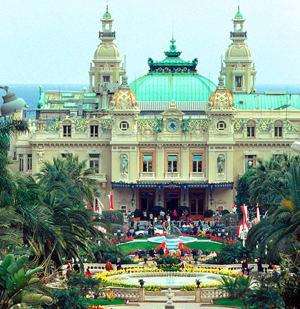
\includegraphics[width=\columnwidth,height=110pt]{monte.jpg}\\
\begin{center}
\begin{tiny}
\vspace*{-6pt}
Image source:\\
\url{http://commons.wikimedia.org/wiki/}\\
File:Monte\_Carlo\_Casino.jpg.\\
Used under the license given there
\end{tiny}
\end{center}
\end{spacing}
\end{column}
\end{columns}
\newpage
\vspace*{9pt}
Monte Carlo algorithms always yield an output, but it is possible that the
output is false. The steps involved in these algorithms may be considered
to be similar to gambling, whence the name.\\[6pt]
A Monte Carlo algorithm performs several iterations, or tests, to determine
the truth of some statement. Each test will give either ``true'' or
``unknown''. If at least one of the tests yields ``true'', the algorithm will
output ``true''. If all the tests yield ``unknown'', then the algorithm will
output ``false''.\\[6pt]
The probability that the actual statement is true but a test yields
``unknown'' instead of ``true'' is small, and by performing many tests, the
probability that the final output is ``false'' while the statement is actually
true can be made very small.
\end{spacing}
\end{frame}
\begin{frame}[t,allowdisplaybreaks,allowframebreaks]{Miller-Rabin Test for Primality}
\begin{spacing}{1.05}
\begin{EXAMPLE}
The Miller-Rabin test is a Monte Carlo Algorithm that
determines whether or not an integer is prime.\\[6pt]
\end{EXAMPLE}
Let $n\in\N$ be an odd integer. Then
\[n-1=2^st\qquad\qquad\text{for some}~s\in\N~\text{and an odd integer }t\in\N.\]
The integer $n$ is said to pass the \emph{Miller-Rabin test to base b} if either
\[b^t\equiv1\,(\text{mod}\,n)\qquad\qquad\quad
\text{or}\qquad\qquad\quad b^{2^jt}\equiv-1\,(\text{mod}\,n)\]
for some $j$ with $0\leq j\leq s-1$.
\begin{itemize}
  \item If $n$ is prime and $1<b<n$, then $n$ passes the Miller-Rabin test to base $b$.
  \item If $n$ is composite, then there are fewer than $n/4$ bases $b$ with $1<b<n$ such that $n$ passes Miller's test to base $b$.
\end{itemize}
\newpage
\vspace*{7pt}
The Monte Carlo algorithm now randomly selects $k$ bases $b$ and performs
the Miller-Rabin test.\\[2pt]
\begin{itemize}
  \item If $n$ fails the test for any of the bases used, the algorithm will return ``true''($n$ is composite).
  \item If $n$ passes each test, the answer is still unknown. Nevertheless, the algorithm will return ``false'' ($n$ is prime).
\end{itemize}
The probability that $n$ is composite and still passes the test each of the $k$
times is
\[p_k=\frac{1}{4^k}.\]
If, e.g., $k=30$ tests are performed, $p_k<10^{-18}$. It is almost certain that a
number that the algorithm returns as prime actually is prime.
\end{spacing}
\end{frame}
\begin{frame}[t]{Quick Sort}
\begin{spacing}{1.1}
Among the different sorting algorithms studied so far the most efficient
one is Merge Sort. However, Merge Sort requires a significant amount of
spatial resources. Furthermore, although Merge Sort is asymptotically
optimal, there are other algorithms that perform better in practice.\\[6pt]
One of these is called \emph{Quick Sort}. Like Merge Sort, it uses a
divide-and-conquer strategy. But instead of merging two lists, Quick Sort
reorders each sublist according to a chosen element:
\begin{itemize}
  \item From a list of elements, choose an element, called the pivot. Often, this is the last element of the list.
  \item Rearrange the list by ordering all elements with values smaller than the pivot to its left and all larger elements to its right.
  \item The pivot is now in its final position and there are two sublists, one on either side.
  \item Recursively apply the above procedure to these two sublists.
\end{itemize}
\end{spacing}
\end{frame}
\begin{frame}[t]{Pseudocode for Quick Sort}
\begin{spacing}{1.1}
\stepcounter{zhuo}
\alert{2.5.15. Algorithm.} \emph{(Quick Sort)}
\IncMargin{1em}
\begin{algorithm}[H]
\SetKwInput{Kw}{Input}\SetKwInput{Kt}{Output}
\SetKwFunction{qsort}{qsort}
\SetKwIF{If}{ElseIf}{Else}{if}{then}{else if}{else}{end~if}
\SetKwFor{For}{for}{do}{end~for}
\SetKwBlock{Function}{Function \qsort{$L,j,k$}:}{end}
\Kw{$L=\langle I_1,\cdots,I_n\rangle$ a list of $n$ elements}
\Kt{$L$ with its elements in increasing order}
\Function{\If{$j<k$}{
\For{$i\leftarrow1$ \KwTo $k-1$}{
\lIf{$I_i<I_k$}{\textbf{swap}\,$I_i$ and $I_j$;\:$j\leftarrow j+1$\;
}}
\textbf{swap}\,$I_j$ and $I_k$\;
\qsort{$L,1,j-1$}; \qsort{$L,j+1,k$}}
\lElse{\Return $L$}}
\end{algorithm}\DecMargin{1em}
\end{spacing}
\end{frame}
\begin{frame}[t]{Quick Sort}
\begin{spacing}{1.2}
\begin{EXAMPLES}
\begin{enumerate}[(i)]
  \item To order the list $L=\langle4,3,1,2\rangle$, 2 is selected as the pivot. The following comparisons are performed: $4\nless 2,\,3\nless 2,\,1<2$. 1 and 4 are swapped, and so are 2 and 3 such that 2 consists of only one element and as such is already ordered. The one on the right of 2 is $\langle4,3\rangle$, which is ordered using one comparison $3<4$. $L=\langle1,2,3,4\rangle$ is now ordered.
  \item To order the list $L=\langle1,2,3,4,5\rangle$, 5 is selected as the initial pivot. Four comparisons are performed $1<5,\,2<5,\,3<5$ and $4<5$. 5 is already in its final position. Only the left sublist with pivot 4 is to be considered, which leads to three comparisons. Then two comparisons for 3 as a pivot and 1 when it is 2. This easily extends to a list of $n$ elements that are already ordered. In this case $\sum_{i=1}^{n-1}i=\frac{n(n-1)}{2}=O(n^2)$ comparisons are performed.
\end{enumerate}
\end{EXAMPLES}
\end{spacing}
\end{frame}
\begin{frame}[c]{Problems of Quick Sort with Fixed Pivot}
\begin{spacing}{1.1}
The second example shows that the worst-case complexity of Quick Sort is
$O(n^2)$. Even worse, the case of a sorted or almost-sorted list is fairly
common in applications, so that this worst case occurs fairly often in
practice. On the other hand, for ``random'' lists, Quick Sort is quite fast.\\[6pt]
While we could decide to choose a different pivot (for example, the first
instead of the last element of a list), this would still leave the algorithm
vulnerable to being slow for certain special cases.\\[6pt]
A better solution is to choose the pivot \emph{randomly}!
\end{spacing}
\end{frame}
\begin{frame}[c]{Las Vegas Algorithms}
\begin{spacing}{1.1}
This leads us to a new type of probabilistic algorithm is called a \emph{Las Vegas
algorithm}, named after the famous desert city in Nevada, US, where
gambling is legal.\\[6pt]
While a Monte Carlo algorithm sometimes returns a wrong result, albeit
with low probability, a Las Vegas algorithm always gives the correct
output. What is random in a Las Vegas algorithm is the \emph{running time} of
the algorithm.\\[6pt]
In a deterministic algorithm, given specified input and the steps of the
algorithm, the time complexity can be calculated precisely. In a Las Vegas
algorithm, even for specified input, this is not possible.\\[6pt]
One often uses Las Vegas algorithms for comparatively small input size,
since for large input their running time can be quite long.
\end{spacing}
\end{frame}
\begin{frame}[t]{Pseudocode for Quick Sort with Random Pivot}
\begin{spacing}{1.1}
\stepcounter{zhuo}
\alert{2.5.17. Algorithm.} \emph{(Quick Sort with Ransom Pivot)}
\IncMargin{1em}
\begin{algorithm}[H]
\SetKwInput{Kw}{Input}\SetKwInput{Kt}{Output}
\SetKwFunction{qsort}{qsort\tt{\_}r}
\SetKwIF{If}{ElseIf}{Else}{if}{then}{else if}{else}{end~if}
\SetKwFor{For}{for}{do}{end~for}
\SetKwBlock{Function}{Function \qsort{$L,j,k$}:}{end}
\Kw{$L=\langle I_1,\cdots,I_n\rangle$ a list of $n$ elements}
\Kt{$L$ with its elements in increasing order}
\Function{\If{$j<k$}{
$r\leftarrow\text{rand}(k)$;\:\textbf{swap}\,
$I_r$ and $I_k$\tcc*[r]{$0<r\leq k$: rand pivot}
\For{$i\leftarrow1$ \KwTo $k-1$}{
\lIf{$I_i<I_k$}{\textbf{swap}\,$I_i$ and $I_j$;\:$j\leftarrow j+1$\;
}}
\textbf{swap}\,$I_j$ and $I_k$\;
\qsort{$L,1,j-1$}; \qsort{$L,j+1,k$}\;}
\lElse{\Return $L$\;}}
\end{algorithm}\DecMargin{1em}
\end{spacing}
\end{frame}
\begin{frame}[t,allowdisplaybreaks,allowframebreaks]{Time Complexity of Quick Sort with Random Pivot}
\begin{spacing}{1.05}
By choosing a random pivot, one essentially forces a given list to be
``random'', even if it is structured in some way originally. Hence, Quick
Sort with a random pivot is equivalent to Quick Sort with a fixed pivot
acting on a randomly ordered list.\\[5pt]
The random pivot serves only to prevent ``worst'' cases (which may be
common practical configurations) from occurring often.\\[5pt]
Therefore, the (worst-case) time complexity of Quick Sort with random
pivot remains $O(n^2)$. However, as we now show, the ``average case'' complexity is $O(n\log n)$.\\[5pt]
Let $t(n)$ denote the number of comparisons needed to Quick Sort a list of $n$ elements. Then
\[t(0)=t(1)=1\]
since lists of one or zero elements are trivially sorted and only one
comparison is needed to find the size of the list.
\newpage
Suppose that the chosen pivot is the $i$th-largest element of the list. Then
\[t(n)=t(i-1)+t(n-i)+n,\qquad\quad i=1,\,...\,,n,\qquad\quad n\geq2.\]
since the left sublist will have length $i - 1$, the right sublist will have
length $n - i$ and $n - 1$ comparisons are needed to place each element into
the appropriate sublist. Furthermore, one comparison is used to check if
the list size is at least two; if not, the contents of the list are returned.\\[3pt]
If the pivot is chosen randomly, the probability that it will be the
$i$th-largest element in the list is equal to $1/n$ for each $i$. We calculate the
average time complexity as the expected number of comparisons by
averaging over all possible sizes of the chosen pivot:
\[\bar{t}(n)=\frac{1}{n}\sum_{i=1}^{n}\big(
\bar{t}(i-1)+\bar{t}(n-i)\big)+n\]
\end{spacing}
\newpage
\begin{spacing}{0.8}
Since
\[\sum_{i=1}^{n}\bar{t}(i-1)=\sum_{i=1}^{n}\bar{t}
(n-i)\]
(only the order of summation is reversed) we see that
\[\bar{t}(n)=\frac{2}{n}\sum_{i=1}^{n}
\bar{t}(i-1)+n.\]
Multiplying by $n$, we obtain
\begin{equation}\label{2.5.5}
n\cdot\bar{t}(n)=2\sum_{i=1}^{n}\bar{t}(i-1)+n^2
\end{equation}
We also have
\begin{equation}\label{2.5.6}
(n-1)\cdot\bar{t}(n-1)=2\sum_{i=1}^{n-1}\bar{t}(i-1)+(n-1)^2
\end{equation}
\end{spacing}
\newpage
\begin{spacing}{1}
Subtracting \eqref{2.5.6} from \eqref{2.5.5},
\[n\cdot\bar{t}(n)-(n-1)\cdot\bar{t}(n-1)=2\bar{t}(n-1)+2n-1\]
or
\[\frac{1}{n+1}\bar{t}(n)=\frac{1}{n}\bar{t}(n-1)
+\frac{2}{n+1}\]
This is a linear, inhomogeneous, first-order recurrence relation with
variable coefficients. To find a solution, we substitute:
\begin{equation*}
  \begin{split}
     \frac{\bar{t}(n)}{n+1} &=\frac{\bar{t}(n-1)}{n}+\frac{2}{n+1}
     =\frac{\bar{t}(n-2)}{n-1}+\frac{2}{n}+
     \frac{2}{n+1} \\
       &~\vdots \\
       &=\frac{t(1)}{2}+2\sum_{k=1}^{n+1}\frac{1}{k}.
  \end{split}
\end{equation*}
\newpage
Since
\[\frac{1}{k}\leq\int_{k-1}^{k}\frac{1}{x}dx,\qquad\qquad\qquad\qquad
k\geq2,\]
we have
\begin{equation*}
  \begin{split}
     \frac{\bar{t}(n)}{n+1} &\leq\frac{1}{2}+2+2\sum_{k=2}^{n+1}\int_{k}^{k-1}\frac{1}{x}dx \\
       &=\frac{1}{2}+2+2\int_{1}^{n+1}\frac{1}{x}dx \\
       &=\frac{1}{2}+2+2\ln(n+1) \\
       &=O(\log n)
  \end{split}
\end{equation*}
and hence
\[\bar{t}(n)=O(n\log n).\]
\end{spacing}
\end{frame}
\begin{frame}[t]{Worst-Case and Average-Case Time Complexity}
\begin{spacing}{1.1}
This shows our assertion: that \emph{on average}, Quick Sort needs $O(n \log n)$
comparisons to sort a list. This is true no matter whether the pivot is
chosen randomly or deterministically. Random choice of pivot only serves
to prevent common worst-case scenarios from occurring often.\\[5pt]
Let us summarize several issues that we need to be aware of when
discussing time complexity:
\begin{itemize}
  \item Time complexity does not make any statement about the spatial resources required.
  \item Complexity expressed using Landau symbols is an \emph{asymptotic statement}. For finite $n$, an algorithm that is asymptotically slow can be very fast.
  \item Complexity as we have previously calculated it is actually \emph{worst-case complexity}. An algorithm with bad worst-case complexity may still be very useful in practice, if the worst case occurs very rarely. For that reason, \emph{average-case} complexity is often at least as important as worst-case complexity.
\end{itemize}
\end{spacing}
\end{frame}
\begin{frame}[t,allowdisplaybreaks,allowframebreaks]{The Probabilistic Method}
\begin{spacing}{1.05}
The probabilistic method is a technique for showing the existence of
objects with specified properties. It is non-constructive, i.e., it does not
give information on how to find/construct these objects but only
establishes that they exist.\\[5pt]
The method is based on assigning probabilities to all elements of a set $S$.
An object with specified properties exists in $S$ if its probability is greater
than zero.\\[5pt]
\stepcounter{zhuo}
\alert{2.5.18. Probabilistic Method.} If the probability that an element of a set $S$
does not have a specified property is less than 1, then there exists an
element in $S$ with this property.\\[5pt]
As a demonstration, we will prove the following statement:\\[4pt]
\begin{EXAMPLE}
Let $k\in\N\setminus\{0,1\}$. Then $R(k,k)\geq 2^{k/2}$, where $R$ denotes the Ramsey number introduced on Slide \hyperlink{386}{386}.
\end{EXAMPLE}
\newpage
It is clear that this statement is true for $k=2$ and $k=3$, since $R(2,2)=2=2^{2/2}$ and $R(3,3)=6>2^{3/2}$. We will use the probabilistic method to show that if a party has $n<2^{k/2}$ members, it is possible that
no $k$ members are mutual friends or enemies.\\[5pt]
Suppose that a party of $n$ people is assembled randomly in such a way that
it is equally likely for any two people at the party to be friends or enemies. There are $\binom{n}{k}$ different sets of $k$ people at this party, which we denote by $S_1,S_2,\,...\,,S_{\binom{n}{k}}$. Let $E_i$ be the event that all $k$ members of $S_i$ are either mutual friends or enemies. Then the probability that there are either $k$
mutual friends or enemies in $S$ is
\[P[\text{there exist $k$ mutual friends or enemies}]=P\Big[\bigcup_{i=1}^{\binom{n}{k}}E_i\Big].\]
\newpage
There are $\binom{k}{2}=k(k-1)/2$ pairs of people in each $S_i$, and the probability that they are enemies is $1/2$. Thus, the probability that all members if $S_i$ are enemies is $2^{-k(k-1)/2}$. The probability that they are all friends is also $2^{-k(k-1)/2}$, so
\[P[E_i]=2\cdot2^{-k(k-1)/2}.\]
Using Boole's inequality \eqref{2.5.2} and $\binom{n}{k}\leq n^k/2^{k-1}$ (see assignments),
\[P\Big[\bigcup_{i=1}^{\binom{n}{k}}E_i\Big]\leq
\sum_{i=1}^{\binom{n}{k}}P[E_i]\leq 2^{1-k(k-1)/2}\frac{n^k}{2^{k-1}}=2^{2-k/2}\frac{n^k}{2^{k^2/2}}.\]
Now if $n<2^{k/2}$ and $k>4$,
\[P\Big[\bigcup_{i=1}^{\binom{n}{k}}E_i\Big]<1.\]
\newpage
\vspace*{9pt}
We have therefore shown that for a party whose members are randomly
assigned friendship or enmity with each other,
\[P[\text{there exist $k$ mutual friends or enemies in a party of $n$ members}]<1.\]
However, by Definition 2.5.1,
\begin{align*}
  &P[\text{there exist $k$ mutual friends or enemies in a party of $n$ members}] \\
  =&\frac{\text{number of parties containing groups of $k$ mutual friends/enemies}}{\text{number of all possible parties with $n$ members}}
\end{align*}
Since the quotient is less than 1 if $n<2^{k/2}$ and $k>4$ it follows that there must exist some party of $n$ members not containing a group of $k$ mutual friends or enemies and we see that $R(k,k)\geq2^{k/2}$.
\end{spacing}
\end{frame}
\begin{frame}[c]{Second Midterm Exam}
\begin{spacing}{1.1}
This concludes the material that will be covered in the second midterm
exam. The material is based on the following textbook chapters:
\begin{itemize}
  \item Chapter 4, Section 3;
  \item Chapter 5;
  \item Chapter 6, Sections 1 and 2;
  \item Chapter 7.
\end{itemize}
Some of the material (such as cryptographic algorithms) may not appear
in this form in the textbook; it is nevertheless part of the exam. The
above textbook chapters are for reference only. The lecture slides and
assignments represent the definitive exam material.\\[6pt]
For the exam, you \textcolor[rgb]{1.00,0.00,0.00}{\textbf{may not}} bring a calculator or any other electronic
device, such as a cellphone or electronic dictionary. A monolingual
dictionary in the form of a paper book is allowed.
\end{spacing}
\end{frame}
\section{Selected Topics of Discrete Mathematics}
\begin{frame}
\begin{center}
  \LARGE{Part III}\\ \alert{Selected Topics of Discrete Mathematics}
\end{center}
\end{frame}
\begin{frame} \begin{spacing}{2.5}
\tableofcontents[currentsubsection,hideothersubsections,sectionstyle=hide]
\end{spacing}
\end{frame}
\subsection{Graphs}
\begin{frame}[c] \begin{spacing}{2.5}
\tableofcontents[sectionstyle=hide,subsectionstyle=show/shaded/hide] \end{spacing}
\end{frame}
\begin{frame}[t]{Graphs}
\begin{spacing}{1.1}
\begin{DEFINITION}
A pair $G=(V,E)$ is said to be an \emph{(undirected) graph} if
\begin{itemize}
  \item $V$ is a non-empty set of objects called \emph{vertices}.
  \item $E$ is a set or multiset of one- or two-element subsets of $V$ called \emph{edges}. One-element subsets are called \emph{loops}.
\end{itemize}
The set $V$ is called the \emph{vertex set}, $E$ the \emph{edge set} of $G$.\\[5pt]
An edge $e=\{u,v\}\in E$ with $u,v\in V,\,u\neq v$, is said to \emph{connect} the \emph{endpoints} $u$ and $v$.\\[5pt]
If $\text{card}\,V<\infty$ we say that $G$ is a \emph{finite graph}, otherwise an infinite graph.\\[5pt]
If $E$ is a set (every element of $E$ occurs at most once) and does not contain one-element sets, then $G$ is said to be a \emph{simple graph}.\\[5pt]
If $E$ is a multiset, $G$ is said to be a \emph{multigraph}.\\[5pt]
If $E$ contains one-element subsets of $V$, $G$ is said to be a \emph{pseudograph}.
\end{DEFINITION}
\end{spacing}
\end{frame}
\begin{frame}[t,allowdisplaybreaks,allowframebreaks]{Drawing Graphs}
\begin{spacing}{1.1}
We usually represent a graph by drawing the vertices as points and the
edges as lines joining the vertices. For example, the graph $G=(V,E)$ with
\begin{align*}
  V &=\{a,b,c,d,e\}, \\
  E &=\big\{\{a,b\},\{b,c\},\{a,c\},\{a,d\},\{d,e\},\{b,e\}\big\}
\end{align*}
can be represented as
\begin{center}
\tikzset{
my state/.style={circle,draw,thick}}
 \begin{tikzpicture}[node distance=2cm,on grid,
every state/.style={draw=black,fill=white,text=black,very thick}]
\node[my state] (A) {$a$};
 \node[my state] (B) [right=of A] {$b$};
 \node[my state] (C) [below=of B] {$c$};
 \node[my state] (D) [below=of A] {$d$};
 \node[my state] (E) [left=of D] {$e$};
 \path[-,line width=0.35mm] (A) edge  node{}(B)
           edge  node{}(C)
           edge  node{}(D)
       (B) edge  node{}(C)
           edge  node{}(E)
       (D) edge  node{}(E);
\end{tikzpicture}
\end{center}
\newpage
Below are drawing of a multigraph and a pseudograph:\\[7pt]
\begin{columns}[totalwidth=\textwidth]
\begin{column}{0.5\textwidth}
\begin{center}
\tikzset{
my state/.style={circle,draw,thick}}
\begin{tikzpicture}[node distance=2cm,on grid,
every state/.style={draw=black,fill=white,text=black,very thick}]
\node[my state] (A) {$a$};
 \node[my state] (B) [right=of A] {$b$};
 \node[my state] (C) [below=of B] {$c$};
 \node[my state] (D) [below=of A] {$d$};
 \node[my state] (E) [below=of D] {$e$};
 \path[-,line width=0.35mm] (A) edge  node{}(B)
           edge  node{}(C)
           edge  node{}(D)
       (B) edge  node{}(C)
           edge[bend left]  node{}(D)
           edge[bend right] node{}(D)
       (D) edge[bend left]  node{}(E)
           edge[bend right] node{}(E);
\end{tikzpicture}
\end{center}
\end{column}
\begin{column}{0.5\textwidth}
\vspace*{-6pt}
\begin{center}
\tikzset{
my loop/.style={to path={
.. controls +(45:1.5) and +(315:1.5) .. (\tikztotarget) \tikztonodes}},
my loop2/.style={to path={
.. controls +(225:1.5) and +(315:1.5) .. (\tikztotarget) \tikztonodes}},
my state/.style={circle,draw,thick}}
\begin{tikzpicture}[node distance=2cm,on grid,
every state/.style={draw=black,fill=white,text=black,very thick}]
\node[my state] (A) {$a$};
 \node[my state] (B) [right=of A] {$b$};
 \node[my state] (C) [below=of B] {$c$};
 \node[my state] (D) [below=of A] {$d$};
 \node[my state] (E) [below=of D] {$e$};
 \path[-,line width=0.35mm] (A) edge  node{}(B)
           edge  node{}(C)
           edge  node{}(D)
       (B) edge  node{}(C)
           edge[bend left]  node{}(D)
           edge[bend right] node{}(D)
       (D) edge  node{}(E);
 \draw[-,line width=0.35mm] (B) to [my loop] node[]{}(B);
 \draw[-,line width=0.35mm] (C) to [my loop2] node[]{}(C);
\end{tikzpicture}
\end{center}
\end{column}
\end{columns}
\end{spacing}
\end{frame}
\begin{frame}[t,allowdisplaybreaks,allowframebreaks]{Directed Graphs}
\begin{spacing}{1.1}
\begin{DEFINITION}
A pair $G=(V,E)$ is said to be a \emph{directed graph} or \emph{digraph} if
\begin{itemize}
  \item $V$ is a non-empty set of objects called \emph{vertices}.
  \item $E$ is a set or multiset of pairs of elements of $V$ called \emph{directed edges} or \emph{arcs}.
\end{itemize}
An edge $e=\{u,v\}\in E$ with $u,v\in V,u\neq v$, is said to \emph{start at u} and \emph{end at v}.\\[5pt]
If $\text{card}\,V<\infty$ we say that $G$ is a \emph{finite directed graph}, otherwise an infinite directed graph.\\[5pt]
If $E$ is a set (every element of $E$ occurs at most once) and does not contain
pairs with equal components, then $G$ is said to be a \emph{simple directed graph}.
If $E$ is a multiset or contains pairs with equal components, $G$ is said to be
a \emph{directed multigraph}.
\end{DEFINITION}
\newpage
\begin{REMARK}
Note that while a directed multigraph may contain loops,
an undirected multigraph may not (such an undirected graph would be
called a pseudograph). Since graph theory is still a fairly young discipline,
the terminology used varies widely and is not always logical or consistent.\\[7pt]
\end{REMARK}
\begin{EXAMPLE}
A simple directed graph and a directed multigraph\\[8pt]
\end{EXAMPLE}
\begin{center}
\tikzset{
my state/.style={circle,draw,thick}}
  \begin{tikzpicture}[node distance=2cm,on grid,
every state/.style={draw=black,fill=white,text=black,very thick}]
\node[my state] (A) {$a$};
 \node[my state] (B) [right=of A] {$b$};
 \node[my state] (C) [below=of B] {$c$};
 \node[my state] (D) [below=of A] {$d$};
 \path[->,>=stealth,line width=0.35mm] (A) edge  node{}(B)
           edge  node{}(D)
       (C) edge  node{}(A)
           edge  node{}(B);
\end{tikzpicture}
\qquad\qquad\qquad
\tikzset{
my loop/.style={to path={
.. controls +(315:1.5) and +(45:1.5) .. (\tikztotarget) \tikztonodes}},
my state/.style={circle,draw,thick}}
  \begin{tikzpicture}[node distance=2cm,on grid,
every state/.style={draw=black,fill=white,text=black,very thick}]
\node[my state] (A) {$a$};
 \node[my state] (B) [right=of A] {$b$};
 \node[my state] (C) [below=of B] {$c$};
 \node[my state] (D) [below=of A] {$d$};
 \path[->,>=stealth,line width=0.35mm] (A) edge  node{}(B)
     edge  node{}(D)
 (B) edge[bend right]  node{}(D)
 (C) edge  node{}(A)
     edge  node{}(B)
 (D) edge[bend right]  node{}(B);
 \draw[->,>=stealth,line width=0.35mm] (B) to [my loop] node[]{}(B);
\end{tikzpicture}
\end{center}
\end{spacing}
\end{frame}
\begin{frame}[t,allowdisplaybreaks,allowframebreaks]{Example: Graphs in Football}
\begin{spacing}{1.05}
\begin{EXAMPLE}
In the group stage of the 2010 World Cup, Group A
consisted of Uruguay, Mexico, South Africa and France. Each of the teams
played against each of the other three teams. (This is called a \emph{round-robin
tournament}.) The following undirected simple graph represents the
matches:
\vspace*{9pt}
\begin{center}
\tikzset{
my state/.style={circle,draw,fill=black}}
  \begin{tikzpicture}[-,auto,node distance=2.7cm,on grid,every state/.style={fill=black,draw=black}]
    \node[my state] (A){};
    \node[my state] (B)[below=of A]{};
    \node[my state] (C)[right=of A]{};
    \node[my state] (D)[below=of C]{};
    \path (A) edge node{}(B)
              edge node{}(C)
              edge node{}(D)
          (B) edge node{}(C)
              edge node{}(D)
          (C) edge node{}(D);
    \node [above left=0.2cm] at (A) {Mexico};
    \node [above right=0.2cm] at (C) {Uruguay};
    \node [below left=0.2cm] at (B) {South Africa};
    \node [below right=0.2cm] at (D) {France};
  \end{tikzpicture}
\end{center}
\end{EXAMPLE}
\newpage
By adding arrows to the edges we can indicate which team eventually won
each match:
\begin{center}
\tikzset{
my state/.style={circle,draw,fill=black}}
  \begin{tikzpicture}[->,>=stealth,auto,node distance=2.7cm,on grid,every state/.style={fill=black,draw=black}]
    \node[my state] (A){};
    \node[my state] (B)[below=of A]{};
    \node[my state] (C)[right=of A]{};
    \node[my state] (D)[below=of C]{};
    \path (A) edge node{}(D)
          (B) edge node{}(D)
          (C) edge node{}(A)
          (C) edge node{}(B);
    \draw[-](A) -- (B);
    \draw[-](C) -- (D);
    \node [above left=0.2cm] at (A) {Mexico};
    \node [above right=0.2cm] at (C) {Uruguay};
    \node [below left=0.2cm] at (B) {South Africa};
    \node [below right=0.2cm] at (D) {France};
  \end{tikzpicture}
\end{center}
The graph shows that Uruguay won its match against Mexico, but drew
against France. A graph containing directed as well as undirected edges is
called a \emph{mixed graph}.
\newpage
Alternatively, we can indicate the goals scored by each team against the
other teams:
\begin{center}
\tikzset{
my state/.style={circle,draw,fill=black}}
  \begin{tikzpicture}[->,>=stealth,auto,node distance=2.7cm,on grid,every state/.style={fill=black,draw=black}]
    \node[my state] (A){};
    \node[my state] (B)[below=of A]{};
    \node[my state] (C)[right=of A]{};
    \node[my state] (D)[below=of C]{};
    \path (A) edge[bend right] node{}(B)
          edge node{}(D)
          edge[bend left] node{}(D)
          (B) edge node{}(A)
              edge node{}(D)
              edge[bend left] node{}(D)
          (C) edge node{}(A)
              edge[bend left] node{}(B)
              edge[bend right] node{}(B)
              edge node{}(B)
          (D) edge[bend left] node{}(B);
    \node [above left=0.2cm] at (A) {Mexico};
    \node [above right=0.2cm] at (C) {Uruguay};
    \node [below left=0.2cm] at (B) {South Africa};
    \node [below right=0.2cm] at (D) {France};
  \end{tikzpicture}
\end{center}
The graph shows that Uruguay did not concede a single goal and scored
three goals against South Africa. The match between France and Uruguay
ended without a goal scored. This is a directed multigraph.
\end{spacing}
\end{frame}
\begin{frame}[c]{Degree of Vertices in an Undirected Graph}
\begin{spacing}{1.2}
\begin{DEFINITION}
Let $G$ be an undirected graph and $\{u,v\}$ and edge of $G$. Then
\begin{itemize}
  \item $\{u,v\}$ is said to be \emph{incident} to $u$ and $v$.
  \item $u$ and $v$ are said to be adjacent.
\end{itemize}
The degree $\deg(v)$ of a vertex $v$ is the sum of the number of edges that are not loops and twice the number of loops incident to $v$.\\[5pt]
A vertex is said to be isolated if it has degree zero.\\[5pt]
A vertex is said to be pendant if it has degree one.\\[5pt]
\end{DEFINITION}
\end{spacing}
\end{frame}
\begin{frame}[t]{Example: Graphs in Football}
\begin{spacing}{1}
\begin{EXAMPLE}
In the group stage of the 2010 World Cup, Group F
consisted of Paraguay, Slovakia, New Zealand and Italy. The following
undirected simple graph represents the matches that did not end in a draw:
\begin{center}
\tikzset{
my state/.style={circle,draw,fill=black}}
  \begin{tikzpicture}[-,auto,node distance=2.7cm,on grid,every state/.style={fill=black,draw=black}]
    \node[my state] (A){};
    \node[my state] (B)[below=of A]{};
    \node[my state] (C)[right=of A]{};
    \node[my state] (D)[below=of C]{};
    \path (A) edge node{}(C)
              edge node{}(D);
    \node [above left=0.2cm] at (A) {Slovakia};
    \node [above right=0.2cm] at (C) {Paraguay};
    \node [below left=0.2cm] at (B) {New Zealand};
    \node [below right=0.2cm] at (D) {Italy};
  \end{tikzpicture}
\end{center}
Here, New Zealand is isolated, while Italy and Paraguay are pendant. The
vertex Slovakia has degree 2. Italy and Slovakia are adjacent, but Italy and
Paraguay are not.
\end{EXAMPLE}
\end{spacing}
\end{frame}
\begin{frame}[t]{The Handshaking Theorem}
\begin{spacing}{0.9}
The sum of the degrees of all the vertices of a graph must equal twice the
number of edges, since each edge ``contributes'' two degrees. Suppose that the graph $G=(V,E)$ has $|E|$ edges. Then
\[2|E|=\sum_{v\in V}\deg v.\]
This is known as the \emph{handshaking theorem}. A slightly less obvious
statement is the following:\\[5pt]
\begin{THEOREM}
An undirected graph has an even number of vertices of
odd degree.\\[4pt]
\begin{PROOF}
Let $V_1$ and $V_2$ be the set of vertices of even and odd degree in $G=(V,E)$, respectively. Then
\[\underbrace{2|E|}_{\text{even}}=\sum_{v\in V_1}\underbrace{\deg v}_{\text{even}}+\sum_{v\in V_2}\underbrace{\deg v}_{\text{odd}}.\]
\end{PROOF}
\end{THEOREM}
\end{spacing}
\end{frame}
\begin{frame}[t]{Degree of Vertices in a Directed Graph}
\begin{spacing}{1.15}
\begin{DEFINITION}
Let $G$ be a directed graph and $(u,v)$ and edge of $G$. Then
\begin{itemize}
  \item $(u,v)$ is said to have \emph{initial vertex u} and \emph{terminal vertex v}.
  \item $u$ and $v$ are said to be adjacent.
\end{itemize}
The \emph{in-degree} of a vertex $v$, denoted $\deg^-(v)$, is the number of edges with $v$ as a terminal vertex. The \emph{out-degree} of a vertex $v$, denoted $\deg^+(v)$, is the number of edges with $v$ as an initial vertex.\\[5pt]
Note that a loop contributes one to both the in- and the out-degree of a
vertex.\\[5pt]
In a digraph $(V, E)$ the sum of the edges is equal to the sum of the
in-degrees and equal to the sum of the out-degrees:
\[|E|=\sum_{v\in V}\deg^-(v)=\sum_{v\in V}\deg^+(v).\]
\end{DEFINITION}
\end{spacing}
\end{frame}
\begin{frame}[c]{Example: Graphs in Football}
\begin{spacing}{1.1}
\begin{EXAMPLE}
In the graph below,
\[\deg^-(\text{Uruguay})=0,\qquad\qquad\qquad
\deg^+(\text{Uruguay})=4.\]
Uruguay and France are the only vertices that are not adjacent.
\begin{center}
\tikzset{
my state/.style={circle,draw,fill=black}}
  \begin{tikzpicture}[->,>=stealth,auto,node distance=2.7cm,on grid,every state/.style={fill=black,draw=black}]
    \node[my state] (A){};
    \node[my state] (B)[below=of A]{};
    \node[my state] (C)[right=of A]{};
    \node[my state] (D)[below=of C]{};
    \path (A) edge[bend right] node{}(B)
          edge node{}(D)
          edge[bend left] node{}(D)
          (B) edge node{}(A)
              edge node{}(D)
              edge[bend left] node{}(D)
          (C) edge node{}(A)
              edge[bend left] node{}(B)
              edge[bend right] node{}(B)
              edge node{}(B)
          (D) edge[bend left] node{}(B);
    \node [above left=0.2cm] at (A) {Mexico};
    \node [above right=0.2cm] at (C) {Uruguay};
    \node [below left=0.2cm] at (B) {South Africa};
    \node [below right=0.2cm] at (D) {France};
  \end{tikzpicture}
\end{center}
\end{EXAMPLE}
\end{spacing}
\end{frame}
\begin{frame}[t]{Complete Graphs}
\begin{spacing}{1.05}
\begin{DEFINITION}
A \emph{complete graph} $K_j,j\in\N\setminus\{0\}$ is the simple graph
with $j$ vertices that contains exactly one edge between each pair of
vertices.\\[5pt]
\end{DEFINITION}
\begin{EXAMPLES}
The complete graphs $K_j,j=1,2,3,4,5,6$:\\[15pt]
\end{EXAMPLES}
\qquad\qquad\quad
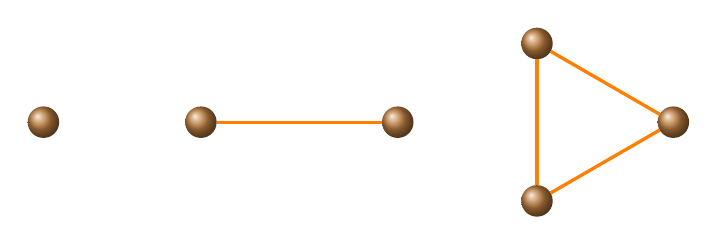
\begin{tikzpicture}
\shade[ball color=brown](-2,0) circle (0.2cm);
\shade[ball color=brown](0,0) circle (0.2cm);
\shade[ball color=brown](2.5,0) circle (0.2cm);
\draw[orange,very thick](0.2,0) -- (2.3,0);
\shade[ball color=brown](6,0) circle (0.2cm);
\shade[ball color=brown](4.26795,1) circle (0.2cm);
\shade[ball color=brown](4.26795,-1)
circle (0.2cm);
\draw[orange,very thick](4.26795,0.8) -- (4.26795,-0.8);
\draw[orange,very thick](4.44116,0.9) -- (5.82679,0.1);
\draw[orange,very thick](4.44116,-0.9) -- (5.82679,-0.1);
\end{tikzpicture}\\[5pt]
\qquad
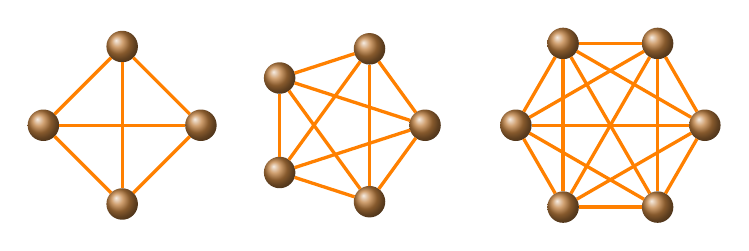
\begin{tikzpicture}
\shade[ball color=brown](0,0) circle (0.2cm);
\shade[ball color=brown](1,1) circle (0.2cm);
\shade[ball color=brown](2,0) circle (0.2cm);
\shade[ball color=brown](1,-1) circle (0.2cm);
\draw[orange,very thick](0.2,0) -- (1.8,0);
\draw[orange,very thick](1,0.8) -- (1,-0.8);
\draw[orange,very thick](0.14142,0.14142) -- (0.85858,0.85858);
\draw[orange,very thick](0.14142,-0.14142) -- (0.85858,-0.85858);
\draw[orange,very thick](1.14142,0.85858) -- (1.85858,0.14142);
\draw[orange,very thick](1.14142,-0.85858) -- (1.85858,-0.14142);
\shade[ball color=brown](3,0.6) circle (0.2cm);
\shade[ball color=brown](3,-0.6) circle (0.2cm);
\shade[ball color=brown](4.14127,0.97082) circle (0.2cm);
\shade[ball color=brown](4.14127,-0.97082) circle (0.2cm);
\shade[ball color=brown](4.8466,0) circle (0.2cm);
\draw[orange,very thick](3,0.4) -- (3,-0.4);
\draw[orange,very thick](3.19021,0.66180) -- (3.95106,0.90901);
\draw[orange,very thick](3.19021,-0.66180) -- (3.95106,-0.90901);
\draw[orange,very thick](4.25883,0.80902) -- (4.72906,0.16180);
\draw[orange,very thick](4.25883,-0.80902) -- (4.72906,-0.16180);
\draw[orange,very thick](4.14127,0.77082) -- (4.14127,-0.77082);
\draw[orange,very thick](3.19021,0.53820) -- (4.65639,0.0618);
\draw[orange,very thick](3.19021,-0.53820) -- (4.65639,-0.0618);
\draw[orange,very thick](3.11756,0.43820) -- (4.02371,-0.80902);
\draw[orange,very thick](3.11756,-0.43820) -- (4.02371,0.80902);
\shade[ball color=brown](6,0) circle (0.2cm);
\shade[ball color=brown](6.6,1.03923) circle (0.2cm);
\shade[ball color=brown](6.6,-1.03923) circle (0.2cm);
\shade[ball color=brown](7.8,1.03923) circle (0.2cm);
\shade[ball color=brown](7.8,-1.03923) circle (0.2cm);
\shade[ball color=brown](8.4,0) circle (0.2cm);
\draw[orange,very thick](6.1,0.17321) -- (6.5,0.86603);
\draw[orange,very thick](6.1,-0.17321) -- (6.5,-0.86603);
\draw[orange,very thick](6.8,1.03923) -- (7.6,1.03923);
\draw[orange,very thick](6.8,-1.03923) -- (7.6,-1.03923);
\draw[orange,very thick](7.9,0.86603) -- (8.3,0.17321);
\draw[orange,very thick](7.9,-0.86603) -- (8.3,-0.17321);
\draw[orange,very thick](6.2,0) -- (8.2,0);
\draw[orange,very thick](6.6,0.83923) -- (6.6,-0.83923);
\draw[orange,very thick](7.8,0.83923) -- (7.8,-0.83923);
\draw[orange,very thick](6.7,0.86602) -- (7.7,-0.86602);
\draw[orange,very thick](6.7,-0.86602) -- (7.7,0.86602);
\draw[orange,very thick](6.17321,0.1) -- (7.62679,0.93923);
\draw[orange,very thick](6.17321,-0.1) -- (7.62679,-0.93923);
\draw[orange,very thick](6.77321,0.93923) -- (8.22680,0.1);
\draw[orange,very thick](6.77321,-0.93923) -- (8.22680,-0.1);
\end{tikzpicture}
\end{spacing}
\end{frame}
\begin{frame}[c]{Cycle Graphs}
\begin{spacing}{1.15}
\begin{DEFINITION}
A \emph{cycle} $C_n,\,n\geq3$, is the graph $G=(V,E)$ with $V=\{v_1,\ldots,v_n\}$ and edges $\{v_j,v_{(j+1)\:\text{mod}\:n}\},\,j=1,\ldots,n$.\\[6pt]
\end{DEFINITION}
\begin{EXAMPLES}
The cycles $C_j,\,j=3,4,5,6$:\\[9pt]
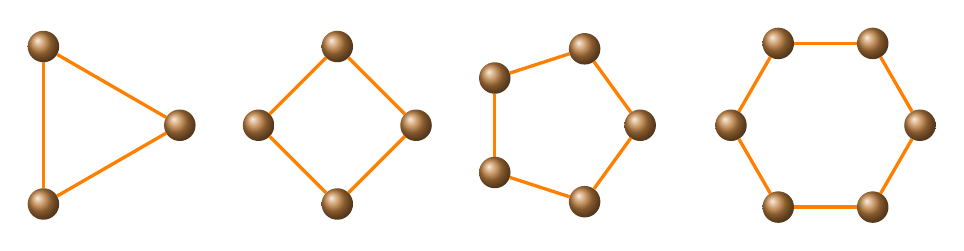
\begin{tikzpicture}
\shade[ball color=brown](6,0) circle (0.2cm);
\shade[ball color=brown](4.26795,1) circle (0.2cm);
\shade[ball color=brown](4.26795,-1)
circle (0.2cm);
\draw[orange,very thick](4.26795,0.8) -- (4.26795,-0.8);
\draw[orange,very thick](4.44116,0.9) -- (5.82679,0.1);
\draw[orange,very thick](4.44116,-0.9) -- (5.82679,-0.1);
\shade[ball color=brown](7,0) circle (0.2cm);
\shade[ball color=brown](8,1) circle (0.2cm);
\shade[ball color=brown](9,0) circle (0.2cm);
\shade[ball color=brown](8,-1) circle (0.2cm);
\draw[orange,very thick](7.14142,0.14142) -- (7.85858,0.85858);
\draw[orange,very thick](7.14142,-0.14142) -- (7.85858,-0.85858);
\draw[orange,very thick](8.14142,0.85858) -- (8.85858,0.14142);
\draw[orange,very thick](8.14142,-0.85858) -- (8.85858,-0.14142);
\shade[ball color=brown](10,0.6) circle (0.2cm);
\shade[ball color=brown](10,-0.6) circle (0.2cm);
\shade[ball color=brown](11.14127,0.97082) circle (0.2cm);
\shade[ball color=brown](11.14127,-0.97082) circle (0.2cm);
\shade[ball color=brown](11.8466,0) circle (0.2cm);
\draw[orange,very thick](10,0.4) -- (10,-0.4);
\draw[orange,very thick](10.19021,0.66180) -- (10.95106,0.90901);
\draw[orange,very thick](10.19021,-0.66180) -- (10.95106,-0.90901);
\draw[orange,very thick](11.25883,0.80902) -- (11.72906,0.16180);
\draw[orange,very thick](11.25883,-0.80902) -- (11.72906,-0.16180);
\shade[ball color=brown](13,0) circle (0.2cm);
\shade[ball color=brown](13.6,1.03923) circle (0.2cm);
\shade[ball color=brown](13.6,-1.03923) circle (0.2cm);
\shade[ball color=brown](14.8,1.03923) circle (0.2cm);
\shade[ball color=brown](14.8,-1.03923) circle (0.2cm);
\shade[ball color=brown](15.4,0) circle (0.2cm);
\draw[orange,very thick](13.1,0.17321) -- (13.5,0.86603);
\draw[orange,very thick](13.1,-0.17321) -- (13.5,-0.86603);
\draw[orange,very thick](13.8,1.03923) -- (14.6,1.03923);
\draw[orange,very thick](13.8,-1.03923) -- (14.6,-1.03923);
\draw[orange,very thick](14.9,0.86603) -- (15.3,0.17321);
\draw[orange,very thick](14.9,-0.86603) -- (15.3,-0.17321);
\end{tikzpicture}
\end{EXAMPLES}
\end{spacing}
\end{frame}
\begin{frame}[c]{Wheel Graphs}
\begin{spacing}{1.15}
\begin{DEFINITION}
A \emph{wheel} $W_n,\,n\geq3$, is the graph $G=(V,E)$ consisting of a cycle $C_n$ with one additional vertex connected to all other vertices.\\[6pt]
\end{DEFINITION}
\begin{EXAMPLES}
The wheels $W_j,\,j=3,4,5,6$:\\[9pt]
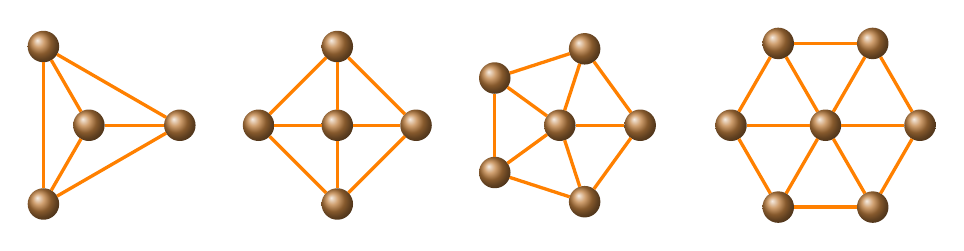
\begin{tikzpicture}
\shade[ball color=brown](6,0) circle (0.2cm);
\shade[ball color=brown](4.26795,1) circle (0.2cm);
\shade[ball color=brown](4.26795,-1)
circle (0.2cm);
\shade[ball color=brown](4.8453,0) circle (0.2cm);
\draw[orange,very thick](4.26795,0.8) -- (4.26795,-0.8);
\draw[orange,very thick](4.44116,0.9) -- (5.82679,0.1);
\draw[orange,very thick](4.44116,-0.9) -- (5.82679,-0.1);
\draw[orange,very thick](5.0453,0) -- (5.8,0);
\draw[orange,very thick](4.36795,0.82679) -- (4.7453,0.17321);
\draw[orange,very thick](4.36795,-0.82679) -- (4.7453,-0.17321);
\shade[ball color=brown](7,0) circle (0.2cm);
\shade[ball color=brown](8,1) circle (0.2cm);
\shade[ball color=brown](9,0) circle (0.2cm);
\shade[ball color=brown](8,-1) circle (0.2cm);
\shade[ball color=brown](8,0) circle (0.2cm);
\draw[orange,very thick](7.14142,0.14142) -- (7.85858,0.85858);
\draw[orange,very thick](7.14142,-0.14142) -- (7.85858,-0.85858);
\draw[orange,very thick](8.14142,0.85858) -- (8.85858,0.14142);
\draw[orange,very thick](8.14142,-0.85858) -- (8.85858,-0.14142);
\draw[orange,very thick](7.2,0) -- (7.8,0);
\draw[orange,very thick](8.2,0) -- (8.8,0);
\draw[orange,very thick](8,0.2) -- (8,0.8);
\draw[orange,very thick](8,-0.2) -- (8,-0.8);
\shade[ball color=brown](10,0.6) circle (0.2cm);
\shade[ball color=brown](10,-0.6) circle (0.2cm);
\shade[ball color=brown](11.14127,0.97082) circle (0.2cm);
\shade[ball color=brown](11.14127,-0.97082) circle (0.2cm);
\shade[ball color=brown](11.8466,0) circle (0.2cm);
\shade[ball color=brown](10.82583,0) circle (0.2cm); % center of the pentagon.
\draw[orange,very thick](10,0.4) -- (10,-0.4);
\draw[orange,very thick](10.19021,0.66180) -- (10.95106,0.90901);
\draw[orange,very thick](10.19021,-0.66180) -- (10.95106,-0.90901);
\draw[orange,very thick](11.25883,0.80902) -- (11.72906,0.16180);
\draw[orange,very thick](11.25883,-0.80902) -- (11.72906,-0.16180);
\draw[orange,very thick](11.02583,0) -- (11.6466,0);
\draw[orange,very thick](10.16180,0.48244) -- (10.66403,0.11756);
\draw[orange,very thick](10.16180,-0.48244) -- (10.66403,-0.11756);
\draw[orange,very thick](10.88763,0.19021) -- (11.07947,0.78061);
\draw[orange,very thick](10.88763,-0.19021) -- (11.07947,-0.78061);
\shade[ball color=brown](13,0) circle (0.2cm);
\shade[ball color=brown](13.6,1.03923) circle (0.2cm);
\shade[ball color=brown](13.6,-1.03923) circle (0.2cm);
\shade[ball color=brown](14.8,1.03923) circle (0.2cm);
\shade[ball color=brown](14.8,-1.03923) circle (0.2cm);
\shade[ball color=brown](15.4,0) circle (0.2cm);
\shade[ball color=brown](14.2,0) circle (0.2cm); % center of the hexagon.
\draw[orange,very thick](13.1,0.17321) -- (13.5,0.86603);
\draw[orange,very thick](13.1,-0.17321) -- (13.5,-0.86603);
\draw[orange,very thick](13.8,1.03923) -- (14.6,1.03923);
\draw[orange,very thick](13.8,-1.03923) -- (14.6,-1.03923);
\draw[orange,very thick](14.9,0.86603) -- (15.3,0.17321);
\draw[orange,very thick](14.9,-0.86603) -- (15.3,-0.17321);
\draw[orange,very thick](13.2,0) -- (14,0);
\draw[orange,very thick](14.4,0) -- (15.2,0);
\draw[orange,very thick](13.7,0.86602) -- (14.1,0.17321);
\draw[orange,very thick](13.7,-0.86602) -- (14.1,-0.17321);
\draw[orange,very thick](14.3,0.17321) -- (14.7,0.86602);
\draw[orange,very thick](14.3,-0.17321) -- (14.7,-0.86602);
\end{tikzpicture}
\end{EXAMPLES}
\end{spacing}
\end{frame}
\begin{frame}[t]{Hypercube Graphs}
\begin{spacing}{1.05}
\begin{DEFINITION}
A \emph{hypercube} $Q_n,\,n\geq1$, is the graph $G=(V,E)$ where $V$ is the set of bit strings of length $n$ and any two vertices are joined by an edge if they differ in a single digit.\\[2pt]
\begin{EXAMPLES}
The cubes $Q_1,\,Q_2,\,Q_3$:\\[10pt]
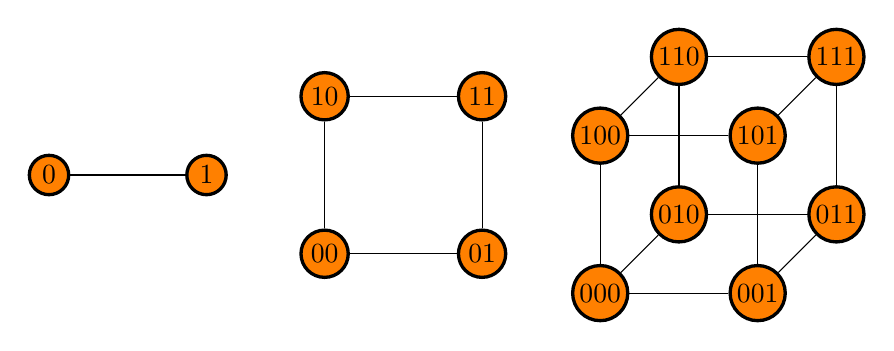
\begin{tikzpicture}[very thick,every node/.style={inner sep=0pt,minimum size=5mm}]
\node (a) at (0,0) [circle,draw=black,fill=orange] {0};
\node (b) at (2,0)
[circle,draw=black,fill=orange] {1};
\draw[-,thin] (a) -- (b);
\node (c) at (3.5,1) [circle,draw=black,fill=orange,minimum size=6mm] {10};
\node (d) at (3.5,-1) [circle,draw=black,fill=orange,minimum size=6mm] {00};
\node (e) at (5.5,1) [circle,draw=black,fill=orange,minimum size=6mm] {11};
\node (f) at (5.5,-1) [circle,draw=black,fill=orange,minimum size=6mm] {01};
\draw[-,thin] (c) -- (d);
\draw[-,thin] (c) -- (e);
\draw[-,thin] (e) -- (f);
\draw[-,thin] (d) -- (f);
\node (g) at (7,-1.5) [circle,draw=black,fill=orange,minimum size=7mm] {000};
\node (h) at (7,0.5) [circle,draw=black,fill=orange,minimum size=7mm] {100};
\node (i) at (9,-1.5) [circle,draw=black,fill=orange,minimum size=7mm] {001};
\node (j) at (9,0.5) [circle,draw=black,fill=orange,minimum size=7mm] {101};
\node (k) at (8,-0.5) [circle,draw=black,fill=orange,minimum size=7mm] {010};
\node (l) at (8,1.5) [circle,draw=black,fill=orange,minimum size=7mm] {110};
\node (m) at (10,1.5) [circle,draw=black,fill=orange,minimum size=7mm] {111};
\node (n) at (10,-0.5) [circle,draw=black,fill=orange,minimum size=7mm] {011};
\draw[-,thin] (g) -- (h);
\draw[-,thin] (g) -- (i);
\draw[-,thin] (g) -- (k);
\draw[-,thin] (l) -- (h);
\draw[-,thin] (l) -- (k);
\draw[-,thin] (l) -- (m);
\draw[-,thin] (j) -- (h);
\draw[-,thin] (j) -- (i);
\draw[-,thin] (j) -- (m);
\draw[-,thin] (n) -- (m);
\draw[-,thin] (n) -- (k);
\draw[-,thin] (n) -- (i);
\end{tikzpicture}\\
A hypercube $Q_n$ can be constructed from two hypercubes $Q_{n-1}$ by prefixing their vertices with zero and 1, respectively, and then joining the vertices that are identical except for the (new) first digit.
\end{EXAMPLES}
\end{DEFINITION}
\end{spacing}
\end{frame}
\begin{frame}[t,allowdisplaybreaks,allowframebreaks]{Bipartite Graphs}
\begin{spacing}{1.05}
\begin{DEFINITION}
A simple graph $G=(V,E)$ is said to be \emph{bipartite} if its vertex set can be partitioned into two disjoint subsets $V_1$ and $V_2$ such that every edge in $E$ connects a vertex in $V_1$ to a vertex in $V_2$. The pair $(V_1,V_2)$ is said to be a \emph{bipartition} of $G$.\\[5pt]
We often write $G=(V_1,V_2,E)$ for a bipartite graph.\\[6pt]
\begin{EXAMPLE}
The cycle $C_6$ is bipartite, while the cycle $C_3$ is not bipartite.\\[5pt]
\begin{center}
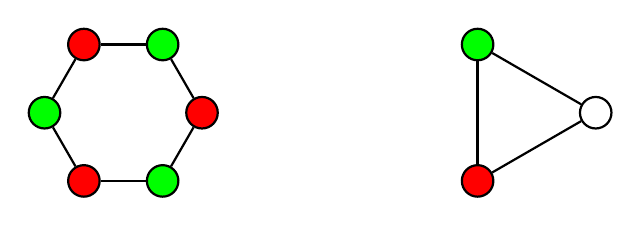
\begin{tikzpicture}[thick,every node/.style={inner sep=0pt,minimum size=4mm}]
\node (a) at (0,0) [circle,draw=black,fill=green] {};
\node (b) at (0.5,0.86603)
[circle,draw=black,fill=red] {};
\node (c) at (0.5,-0.86603)
[circle,draw=black,fill=red] {};
\node (d) at (1.5,0.86603)
[circle,draw=black,fill=green] {};
\node (e) at (1.5,-0.86603)
[circle,draw=black,fill=green] {};
\node (f) at (2,0)
[circle,draw=black,fill=red] {};
\draw[-] (a) -- (b);
\draw[-] (a) -- (c);
\draw[-] (b) -- (d);
\draw[-] (c) -- (e);
\draw[-] (d) -- (f);
\draw[-] (e) -- (f);
\node (g) at (5.5,0.86603) [circle,draw=black,fill=green] {};
\node (h) at (5.5,-0.86603) [circle,draw=black,fill=red] {};
\node (i) at (7,0) [circle,draw=black] {};
\draw[-] (g) -- (h);
\draw[-] (h) -- (i);
\draw[-] (g) -- (i);
\end{tikzpicture}
\end{center}
\end{EXAMPLE}
\end{DEFINITION}
\newpage
Example 3.1.20 suggests the following theorem:\\[5pt]
\begin{THEOREM}
A simple graph is bipartite if and only if it is possible to
assign one of two different colors to each vertex of the graph so that no
two adjacent vertices are assigned the same color.\\[5pt]
\end{THEOREM}
\begin{PROOF}
\begin{itemize}
  \item[($\Rightarrow$)] Assume that the graph $G=(V,E)$ is bipartite. Then $V=V_1\cup V_2$, where every vertex in $V_1$ is adjacent only to an edge in $V_2$ and vice-versa. We assign one color to all vertices in $V_1$ and the other color to all vertices in $V_2$.
  \item[($\Leftarrow$)] Suppose that $G=(V,E)$ and $V=V_1\cup V_2$, where $V_1$ consist of vertices of one color and $V_2$ consists of vertices of the other color and no two vertices of the same color are adjacent. Then every vertex in $V_1$ is adjacent only to a vertex in $V_2$ and vice-versa, so $(V_1,V_2)$ is a bipartition of $G$.
\end{itemize}
\end{PROOF}
\end{spacing}
\end{frame}
\begin{frame}[t]{Complete Bipartite Graphs}
\begin{spacing}{1.05}
Recall from Definition 3.1.11 that a complete graph is a graph where any
two vertices are connected by exactly one edge.\\[6pt]
\begin{DEFINITION}
The \emph{complete bipartite graph} $K_{m,n},\,m,n\in\N\setminus\{0\}$, is a simple graph having a bipartition $(V_1,V_2)$ such that $|V_1|=m,\,|V_2|=n$, and every vertex in $V_1$ is adjacent to every vertex in $V_2$.\\[6pt]
\begin{EXAMPLE}
Below are two ways of drawing the graph $K_{3,3}$:
\begin{center}
 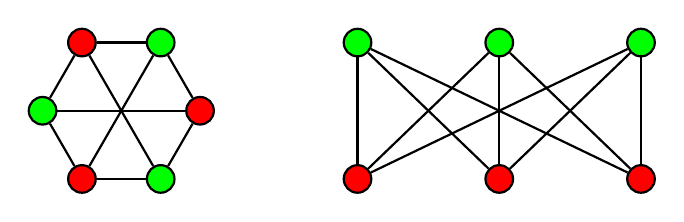
\begin{tikzpicture}[thick,every node/.style={inner sep=0pt,minimum size=3.5mm}]
\node (a) at (0,0) [circle,draw=black,fill=green] {};
\node (b) at (0.5,0.86603)
[circle,draw=black,fill=red] {};
\node (c) at (0.5,-0.86603)
[circle,draw=black,fill=red] {};
\node (d) at (1.5,0.86603)
[circle,draw=black,fill=green] {};
\node (e) at (1.5,-0.86603)
[circle,draw=black,fill=green] {};
\node (f) at (2,0)
[circle,draw=black,fill=red] {};
\draw[-] (a) -- (b);
\draw[-] (a) -- (c);
\draw[-] (b) -- (d);
\draw[-] (c) -- (e);
\draw[-] (d) -- (f);
\draw[-] (e) -- (f);
\draw[-] (a) -- (f);
\draw[-] (b) -- (e);
\draw[-] (c) -- (d);
\node (g) at (4,0.86603) [circle,draw=black,fill=green] {};
\node (h) at (5.8,0.86603) [circle,draw=black,fill=green] {};
\node (i) at (7.6,0.86603) [circle,draw=black,fill=green] {};
\node (j) at (4,-0.86603) [circle,draw=black,fill=red] {};
\node (k) at (5.8,-0.86603) [circle,draw=black,fill=red] {};
\node (l) at (7.6,-0.86603) [circle,draw=black,fill=red] {};
\draw[-] (g) -- (j);
\draw[-] (g) -- (k);
\draw[-] (g) -- (l);
\draw[-] (h) -- (j);
\draw[-] (h) -- (k);
\draw[-] (h) -- (l);
\draw[-] (i) -- (j);
\draw[-] (i) -- (k);
\draw[-] (i) -- (l);
 \end{tikzpicture}
\end{center}
\end{EXAMPLE}
\end{DEFINITION}
\end{spacing}
\end{frame}
\begin{frame}[t,allowdisplaybreaks,allowframebreaks]{Some Applications of Graphs}
\begin{spacing}{1.05}
\begin{EXAMPLE}
Local-Area Networks (LANs) are interconnections of
computers or computing devices (such as printers, routers etc.). There are
three basic ways (topologies) of arranging the network connections,
represented through graphs:\\[7pt]
\begin{columns}[onlytextwidth]
\begin{column}{0.33\textwidth}
\begin{center}
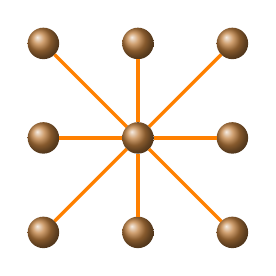
\begin{tikzpicture}
\shade[ball color=brown](0,0) circle (0.2cm);
\shade[ball color=brown](0,1.2) circle (0.2cm);
\shade[ball color=brown](0,2.4) circle (0.2cm);
\shade[ball color=brown](1.2,0) circle (0.2cm);
\shade[ball color=brown](2.4,0) circle (0.2cm);
\shade[ball color=brown](1.2,1.2) circle (0.2cm);
\shade[ball color=brown](1.2,2.4) circle (0.2cm);
\shade[ball color=brown](2.4,1.2) circle (0.2cm);
\shade[ball color=brown](2.4,2.4) circle (0.2cm);
\draw[orange,very thick](1.4,1.2) -- (2.2,1.2);
\draw[orange,very thick](1.2,1.4) -- (1.2,2.2);
\draw[orange,very thick](0.2,1.2) -- (1,1.2);
\draw[orange,very thick](1.2,0.2) -- (1.2,1);
\draw[orange,very thick](0.14142,0.14142) -- (1.05858,1.05858);
\draw[orange,very thick](0.14142,2.25858) -- (1.05858,1.34142);
\draw[orange,very thick](1.34142,1.34142) -- (2.25858,2.25858);
\draw[orange,very thick](1.34142,1.05858) -- (2.25858,0.14142);
\end{tikzpicture}\\
Star Topology\\
(bipartite complete\\
graph $K_{1,n})$
\end{center}
\end{column}
\begin{column}{0.33\textwidth}
\begin{center}
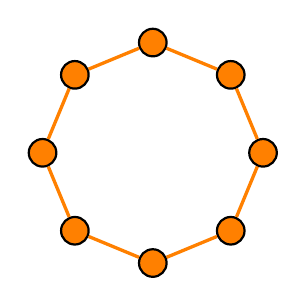
\begin{tikzpicture}[thick,every node/.style={inner sep=0pt,minimum size=3.5mm}]
\node (a) at (1.4,0) [circle,draw=black,fill=orange]{};
\node (b) at (0,1.4) [circle,draw=black,fill=orange]{};
\node (c) at (0,-1.4) [circle,draw=black,fill=orange]{};
\node (d) at (-1.4,0) [circle,draw=black,fill=orange]{};
\node (e) at (0.98995,0.98995) [circle,draw=black,fill=orange]{};
\node (f) at (0.98995,-0.98995) [circle,draw=black,fill=orange]{};
\node (g) at (-0.98995,-0.98995) [circle,draw=black,fill=orange]{};
\node (h) at (-0.98995,0.98995) [circle,draw=black,fill=orange]{};
\draw[-,orange,very thick] (a) -- (e);
\draw[-,orange,very thick] (e) -- (b);
\draw[-,orange,very thick] (b) -- (h);
\draw[-,orange,very thick] (h) -- (d);
\draw[-,orange,very thick] (d) -- (g);
\draw[-,orange,very thick] (g) -- (c);
\draw[-,orange,very thick] (c) -- (f);
\draw[-,orange,very thick] (f) -- (a);
\end{tikzpicture}\\
Ring Topology\\
(ring graph $C_n$)
\end{center}
\end{column}
\begin{column}{0.33\textwidth}
\begin{center}
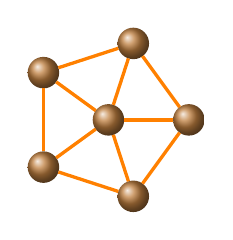
\begin{tikzpicture}
\shade[ball color=brown](10,0.6) circle (0.2cm);
\shade[ball color=brown](10,-0.6) circle (0.2cm);
\shade[ball color=brown](11.14127,0.97082) circle (0.2cm);
\shade[ball color=brown](11.14127,-0.97082) circle (0.2cm);
\shade[ball color=brown](11.8466,0) circle (0.2cm);
\shade[ball color=brown](10.82583,0) circle (0.2cm); % center of the pentagon.
\draw[orange,very thick](10,0.4) -- (10,-0.4);
\draw[orange,very thick](10.19021,0.66180) -- (10.95106,0.90901);
\draw[orange,very thick](10.19021,-0.66180) -- (10.95106,-0.90901);
\draw[orange,very thick](11.25883,0.80902) -- (11.72906,0.16180);
\draw[orange,very thick](11.25883,-0.80902) -- (11.72906,-0.16180);
\draw[orange,very thick](11.02583,0) -- (11.6466,0);
\draw[orange,very thick](10.16180,0.48244) -- (10.66403,0.11756);
\draw[orange,very thick](10.16180,-0.48244) -- (10.66403,-0.11756);
\draw[orange,very thick](10.88763,0.19021) -- (11.07947,0.78061);
\draw[orange,very thick](10.88763,-0.19021) -- (11.07947,-0.78061);
\end{tikzpicture}\\[7pt]
Hybrid Topology\\
(wheel graph $W_n$)
\end{center}
\end{column}
\end{columns}
\end{EXAMPLE}
\end{spacing}
\newpage
\begin{spacing}{1.25}
\begin{EXAMPLE}
In modern computers, calculationally intensive tasks are
not handled by a single processor (\emph{serial processing}) but split into multiple
sub-tasks and handled by several processors concurrently (\emph{parallel
processing}). Since the sub-tasks depend on each other, the processors
need to be connected so that they can communicate with each other. The
processors thus represent a network. The type of connection within the
network will influence the speed of the calculation as well as the type of
parallel software that can be used.\\[6pt]
The simplest possible network would connect any two processors with each
other, forming a complete graph $K_n$ with $\binom{n}{2}$ edges. For 64 processors,
this means there would be 2016 connections and any processor would be
connected to 63 others. This configuration is often not possible in practice
and will always be expensive.
\end{EXAMPLE}
\end{spacing}
\end{frame}
\begin{frame}[c]{Linear Arrays}
\begin{spacing}{1.1}
Another simple arrangement is called a \emph{linear array}, where the $i$th
processor is connected to the ($i-1$)st and the ($i + 1$)st processor, except
that the first is only connected to the second, and the last is only
connected to the penultimate processor. If we label our processors $P_1,\,...\,,P_n$, the linear array is shown below:\\[4pt]
\begin{center}
\tikzset{
my state/.style={circle,draw,thick,inner sep=0pt,minimum size=7mm}}
  \begin{tikzpicture}[node distance=2cm,on grid,
every state/.style={draw=black,fill=white,text=black,very thick}]
\node[my state] (A) at (0,0) {$P_1$};
 \node[my state] (B) at (1.5,0) {$P_2$};
 \node[my state] (C) at (3,0) {$P_3$};
 \node[my state] (D) at (4.5,0) {$P_4$};
 \node[my state] (E) at (7.5,0) {$P_n$};
 \draw[-] (A) -- (B);
 \draw[-] (B) -- (C);
 \draw[-] (C) -- (D);
 \draw[-] (D) -- (E);
\end{tikzpicture}
\end{center}
The disadvantage of the linear array is that communication between two
processors requires sending signals across many intermediate processors,
i.e., requiring many \emph{hops}.
\end{spacing}
\end{frame}
\begin{frame}[t]{Mesh Networks}
\begin{spacing}{1.1}
If there are $n=m^2$ processors, they can be arranged in a \emph{mesh}. The processors are labeled $P_{i,j},0\leq i,j\leq m-1$, and each $P_{i,j}$ is connected to $P_{i\pm 1,j\pm 1}$, i.e., four other processors, as long as they are in the mesh.
\begin{columns}[onlytextwidth]
\begin{column}{0.5\textwidth}
\begin{center}
\tikzset{
my state/.style={circle,draw,thick,inner sep=0pt,minimum size=8mm}}
  \begin{tikzpicture}[node distance=2cm,on grid,
every state/.style={draw=black,fill=white,text=black,very thick}]
\node[my state] (A) at (0,0) {$P_{0,0}$};
 \node[my state] (B) at (1.5,0) {$P_{0,1}$};
 \node[my state] (C) at (3,0) {$P_{0,2}$};
 \node[my state] (D) at (4.5,0) {$P_{0,3}$};
 \node[my state] (E) at (0,1.5) {$P_{1,0}$};
 \node[my state] (F) at (0,3) {$P_{2,0}$};
 \node[my state] (G) at (0,4.5) {$P_{3,0}$};
 \node[my state] (H) at (1.5,1.5) {$P_{1,1}$};
 \node[my state] (I) at (1.5,3) {$P_{2,1}$};
 \node[my state] (J) at (1.5,4.5) {$P_{3,1}$};
 \node[my state] (K) at (3,1.5) {$P_{1,2}$};
 \node[my state] (L) at (3,3) {$P_{2,2}$};
 \node[my state] (M) at (3,4.5) {$P_{3,2}$};
 \node[my state] (N) at (4.5,1.5) {$P_{1,3}$};
 \node[my state] (O) at (4.5,3) {$P_{2,3}$};
 \node[my state] (P) at (4.5,4.5) {$P_{3,3}$};
 \draw[-] (A) -- (B);
 \draw[-] (B) -- (C);
 \draw[-] (C) -- (D);
 \draw[-] (A) -- (E);
 \draw[-] (E) -- (F);
 \draw[-] (F) -- (G);
 \draw[-] (G) -- (J);
 \draw[-] (F) -- (I);
 \draw[-] (E) -- (H);
 \draw[-] (J) -- (I);
 \draw[-] (I) -- (H);
 \draw[-] (H) -- (B);
 \draw[-] (J) -- (M);
 \draw[-] (I) -- (L);
 \draw[-] (H) -- (K);
 \draw[-] (M) -- (L);
 \draw[-] (L) -- (K);
 \draw[-] (K) -- (C);
 \draw[-] (M) -- (P);
 \draw[-] (L) -- (O);
 \draw[-] (K) -- (N);
 \draw[-] (P) -- (O);
 \draw[-] (O) -- (N);
 \draw[-] (N) -- (D);
\end{tikzpicture}
\end{center}
\end{column}
\begin{column}{0.5\textwidth}
Nodes at the edges of the network
are only connected to two or three
other nodes.\\[6pt]
There is a generalization of the
mesh network that ensures that every
node is connected to exactly
four other nodes (see exercises).\\[6pt]
Communication between two arbitrary
nodes requires $O(\sqrt{n})=O(m)$ intermediate links.
\end{column}
\end{columns}
\end{spacing}
\end{frame}
\begin{frame}[c]{Hypercube Networks}
\begin{spacing}{1.15}
Many networks with $n=2^m$ nodes are arranged in hypercubes. The
hypercube configuration balances the number of direct connections of each
processor with the number of intermediate connections required for
communication. A hypercube network for $m=3$ is shown below:\\[10pt]
\begin{center}
\tikzset{
my state/.style={circle,draw,thick,inner sep=0pt,minimum size=7mm}}
\begin{tikzpicture}[node distance=2cm,on grid,
every state/.style={draw=black,fill=white,text=black,very thick}]
\node[my state] (AA) at (-1.5,0) {$P_0$};
\node[my state] (A) at (0,0) {$P_1$};
 \node[my state] (B) at (1.5,0) {$P_2$};
 \node[my state] (C) at (3,0) {$P_3$};
 \node[my state] (D) at (4.5,0) {$P_4$};
 \node[my state] (E) at (6,0) {$P_5$};
 \node[my state] (F) at (7.5,0) {$P_6$};
 \node[my state] (G) at (9,0) {$P_7$};
 \draw[-] (AA) -- (A);
 \draw[-] (B) -- (C);
 \draw[-] (D) -- (E);
 \draw[-] (F) -- (G);
 \draw[-] (AA) to [bend right] (B);
 \draw[-] (A) to [bend right] (C);
 \draw[-] (D) to [bend right] (F);
 \draw[-] (E) to [bend right] (G);
 \draw[-] (AA) to [bend right] (D);
 \draw[-] (A) to [bend right] (E);
 \draw[-] (B) to [bend right] (F);
 \draw[-] (C) to [bend right] (G);
\end{tikzpicture}\\[7pt]
\end{center}
This is another representation of the hypercube in Example 3.1.18.
\end{spacing}
\end{frame}
\begin{frame}[c]{Subgraphs}
\begin{spacing}{1.2}
\begin{DEFINITION}
let $G=(V,E)$ be a graph. Then $H=(W,F)$ is called a \emph{subgraph} of $G$ if $W\subset V$ and $F\subset E$. If $H\neq G$ then $H$ is called a \emph{proper subgraph} of $G$.\\[7pt]
\begin{EXAMPLE}
The cycle $C_6$ is a subgraph of the wheel $W_6$ which is a subgraph of the complete graph $K_7$.
\end{EXAMPLE}
\end{DEFINITION}
\end{spacing}
\end{frame}
\begin{frame}[c]{Union of Graphs}
\begin{spacing}{1.05}
\begin{DEFINITION}
Let $G_1=(V_1,E_1)$ and $G_2=(V_2,E_2)$ be graphs. Then the \emph{union} of $G_1$ and $G_2$, denoted by $G_1\cup G_2$, is the simple graph with vertices $V_1\cup V_2$ and edges $E_1\cup E_2$.\\[6pt]
\begin{EXAMPLE}\\[6pt]
\begin{columns}[onlytextwidth]
\begin{column}{0.3\textwidth}
\begin{center}
\tikzset{
my state/.style={circle,draw,thick,inner sep=0pt,minimum size=6mm}}
\begin{tikzpicture}[node distance=2cm,on grid,
every state/.style={draw=black,fill=white,text=black,very thick}]
\node[my state] (A) at (-1,0) {$A$};
\node[my state] (B) at (0,0) {$B$};
 \node[my state] (C) at (1,0) {$C$};
 \node[my state] (D) at (-1,1) {$D$};
 \node[my state] (E) at (0,1) {$E$};
 \node[my state] (F) at (1,1) {$F$};
 \node[my state] (G) at (-1,2) {$G$};
 \node[my state] (H) at (0,2) {$H$};
 \draw[-] (A) -- (B);
 \draw[-] (C) -- (B);
 \draw[-] (D) -- (A);
 \draw[-] (D) -- (G);
 \draw[-] (G) -- (H);
 \draw[-] (H) -- (E);
 \draw[-] (E) -- (B);
 \draw[-] (E) -- (F);
 \draw[-] (F) -- (C);
 \draw[-] (E) -- (C);
\end{tikzpicture}\\[5pt]
$G_1$
\end{center}
\end{column}
\begin{column}{0.4\textwidth}
\begin{center}
\tikzset{
my state/.style={circle,draw,thick,inner sep=0pt,minimum size=6mm}}
\begin{tikzpicture}[node distance=2cm,on grid,
every state/.style={draw=black,fill=white,text=black,very thick}]
\node[my state] (A) at (-1,0) {$A$};
\node[my state] (B) at (0,0) {$B$};
 \node[my state] (C) at (1,0) {$C$};
 \node[my state] (D) at (-1,1) {$D$};
 \node[my state] (F) at (1,1) {$F$};
 \node[my state] (H) at (0,2) {$H$};
 \node[my state] (I) at (1,2) {$I$};
 \draw[-] (A) -- (B);
 \draw[-] (C) -- (B);
 \draw[-] (D) -- (H);
 \draw[-] (I) -- (H);
 \draw[-] (I) -- (F);
 \draw[-] (F) -- (C);
\end{tikzpicture}\\[5pt]
$G_2$
\end{center}
\end{column}
\begin{column}{0.3\textwidth}
\begin{center}
\tikzset{
my state/.style={circle,draw,thick,inner sep=0pt,minimum size=6mm}}
\begin{tikzpicture}[node distance=2cm,on grid,
every state/.style={draw=black,fill=white,text=black,very thick}]
\node[my state] (A) at (-1,0) {$A$};
\node[my state] (B) at (0,0) {$B$};
 \node[my state] (C) at (1,0) {$C$};
 \node[my state] (D) at (-1,1) {$D$};
 \node[my state] (E) at (0,1) {$E$};
 \node[my state] (F) at (1,1) {$F$};
 \node[my state] (G) at (-1,2) {$G$};
 \node[my state] (H) at (0,2) {$H$};
 \node[my state] (I) at (1,2) {$I$};
 \draw[-] (A) -- (B);
 \draw[-] (C) -- (B);
 \draw[-] (D) -- (A);
 \draw[-] (D) -- (G);
 \draw[-] (G) -- (H);
 \draw[-] (H) -- (E);
 \draw[-] (E) -- (B);
 \draw[-] (E) -- (F);
 \draw[-] (F) -- (C);
 \draw[-] (E) -- (C);
 \draw[-] (D) -- (H);
 \draw[-] (H) -- (I);
 \draw[-] (I) -- (F);
\end{tikzpicture}\\[5pt]
$G_1\cup G_2$
\end{center}
\end{column}
\end{columns}
\end{EXAMPLE}
\end{DEFINITION}
\end{spacing}
\end{frame}
\begin{frame}[t,allowdisplaybreaks,allowframebreaks]{Adjacency Tables}
\begin{spacing}{1.1}
We will now introduce several ways of representing finite graphs. A simple
way to do so is using an \emph{adjacency table}, which lists all the vertices of the
graph and the vertices adjacent to them.\\[6pt]
\begin{EXAMPLE}
The following is a simple graph and its adjacency table:\\[5pt]
\begin{columns}[onlytextwidth]
\begin{column}{0.5\textwidth}
\begin{center}
\tikzset{
my state/.style={circle,draw,thick,inner sep=0pt,minimum size=5.5mm}}
\begin{tikzpicture}[node distance=2cm,on grid,
every state/.style={draw=black,fill=white,text=black,very thick}]
\node[my state] (C) at (0,1.2) {$C$};
\node[my state] (D) at (0,-1.2) {$D$};
 \node[my state] (B) at (2.28254,1.94164) {$B$};
 \node[my state] (E) at (2.28254,-1.94164) {$E$};
 \node[my state] (A) at (3.6932,0) {$A$};
 \draw[-] (A) -- (B);
 \draw[-] (A) -- (C);
 \draw[-] (A) -- (E);
 \draw[-] (C) -- (D);
 \draw[-] (C) -- (E);
 \draw[-] (D) -- (E);
\end{tikzpicture}
\end{center}
\end{column}
\begin{column}{0.5\textwidth}
\begin{tabular}{cc}
  \toprule
  Vertex & Adjacent Vertices \\ \midrule
  A & B,\:C,\:E \\
  B & A \\
  C & A,\:D,\:E \\
  D & C,\:E \\
  E & A,\:C,\:D \\
  \toprule
\end{tabular}
\end{column}
\end{columns}
\end{EXAMPLE}
\newpage
A similar table can be used for directed graphs.\\[6pt]
\begin{EXAMPLE}
The following is a directed graph and its adjacency table:\\[6pt]
\begin{columns}[onlytextwidth]
\begin{column}{0.5\textwidth}
\begin{center}
\tikzset{
my loop/.style={to path={
.. controls +(45:1.5) and +(135:1.5) .. (\tikztotarget) \tikztonodes}},
my state/.style={circle,draw,thick,inner sep=0pt,minimum size=5.5mm}}
\begin{tikzpicture}[->,>=stealth,line width=0.2mm,node distance=2cm,on grid,
every state/.style={draw=black,fill=white,text=black,very thick}]
\node[my state] (C) at (0,1.2) {$C$};
\node[my state] (D) at (0,-1.2) {$D$};
 \node[my state] (B) at (2.28254,1.94164) {$B$};
 \node[my state] (E) at (2.28254,-1.94164) {$E$};
 \node[my state] (A) at (3.6932,0) {$A$};
 \draw (A) to (B);
 \draw (A) to (D);
 \draw (A) to (E);
 \draw (A) [bend right] to (C);
 \draw (B) to (D);
 \draw (C) -- (A);
 \draw (C) [bend right] to (E);
 \draw (E) -- (D);
 \draw (E) -- (C);
 \draw (E) -- (B);
 \draw (B) to [my loop] node[]{}(B);
 \draw (C) to [my loop] node[]{}(C);
\end{tikzpicture}
\end{center}
\end{column}
\begin{column}{0.5\textwidth}
\begin{tabular}{cc}
  \toprule
  Initial Vertex & Terminal Vertices \\ \midrule
  A & B,\:C,\:D,\:E \\
  B & B,\:D \\
  C & A,\:C,\:E \\
  D &   \\
  E & B,\:C,\:D \\
  \toprule
\end{tabular}
\end{column}
\end{columns}
\end{EXAMPLE}
\end{spacing}
\end{frame}
\begin{frame}[t,allowdisplaybreaks,allowframebreaks]{Adjacency Matrices}
\begin{spacing}{1.05}
Instead of tables, matrices can also be used to describe graphs. Assume
that $G=(V,E)$, where $V=(v_1,\,...\,,v_n)$ has been ordered in some way. We then define the \emph{adjacency matrix} $A_G$ by
\[A_G=(a_{ij})_{i,j=1}^n,\qquad\qquad\qquad
a_{ij}=\begin{cases}
         1, & \mbox{if }\{v_i,v_j\}\in E,  \\
         0, & \mbox{otherwise}.
       \end{cases}\]
Note that the adjacency matrix is always symmetric, i.e., $a_{ij}=a_{ji}$.\\[5pt]
\begin{EXAMPLE}
The following is a simple graph and its adjacency matrix:\\[5pt]
\begin{columns}[onlytextwidth]
\begin{column}{0.5\textwidth}
\begin{center}
\tikzset{
my state/.style={circle,draw,thick,inner sep=0pt,minimum size=5.5mm}}
\begin{tikzpicture}[node distance=2cm,on grid,
every state/.style={draw=black,fill=white,text=black,very thick}]
\node[my state] (C) at (0,0.6) {$v_3$};
\node[my state] (D) at (0,-0.6) {$v_4$};
 \node[my state] (B) at (1.14127,0.97082) {$v_2$};
 \node[my state] (E) at (1.14127,-0.97082) {$v_5$};
 \node[my state] (A) at (1.8466,0) {$v_1$};
 \draw[-] (A) -- (B);
 \draw[-] (A) -- (C);
 \draw[-] (A) -- (E);
 \draw[-] (C) -- (D);
 \draw[-] (C) -- (E);
 \draw[-] (D) -- (E);
\end{tikzpicture}
\end{center}
\end{column}
\begin{column}{0.5\textwidth}
$A_G=\bordermatrix{%
& v_1 & v_2 & v_3 & v_4 & v_5 \cr
v_1 & 0 & 1 & 1 & 0 & 1 \cr
v_2 & 1 & 0 & 0 & 0 & 0 \cr
v_3 & 1 & 0 & 0 & 1 & 1 \cr
v_4 & 0 & 0 & 1 & 0 & 1 \cr
v_5 & 1 & 0 & 1 & 1 & 0 \cr
}$
\end{column}
\end{columns}
\end{EXAMPLE}
\newpage
\vspace*{9pt}
In the case of simple graphs, adjacency matrices are zero-one matrices
with vanishing trace. However, they can also be used to describe
multigraphs and pseudographs, in which case the entries $a_{ij}$ are equal to
the multiplicity of the edge $\{v_i,v_j\}$. The adjacency matrix remains
symmetric for any type of undirected graph.\\[7pt]
An adjacency matrix $A_G$ for a directed graph $G=(V,E)$ with $\text{card}\,V=n$ is defined by
\[A_G=(a_{ij})_{i,j=1}^n,\qquad\qquad\qquad
a_{ij}=\begin{cases}
         1, & \mbox{if }(v_i,v_j)\in E, \\
         0, & \mbox{otherwise}.
       \end{cases}\]
Clearly, it does not need to be symmetric.
\newpage
\vspace*{9pt}
For $\text{card}\,V=n$, an adjacency matrix will contain $n^2$ entries, while an adjacency table will have $c\cdot n$ entries, where $c=\max\limits_{1\leq i\leq n}\deg(v_i)$.\\[6pt]
Therefore, if a graph has only few edges, $c\ll n$, (it is \emph{sparse}) it may be
more efficient to use adjacency tables to describe the graph. On the other
hand, in this case most of the entries of the adjacency matrix will be zero
(such a matrix is also called sparse) and there are special techniques to
work with sparse matrices efficiently.\\[6pt]
If the graph is \emph{dense} (contains many edges) it is preferable to use an
adjacency matrix instead of an adjacency table as information is contained
in a more accessible form in the matrix.
\end{spacing}
\end{frame}
\begin{frame}[t]{Incidence Matrices}
\begin{spacing}{1.05}
Graphs can also be represented using \emph{incidence matrices}. If $G=(V,E)$ is an undirected (pseudo-)graph, $V=\{v_1,\,...\,,v_n\}$, and $E=\{e_1,\,...\,,e_m\}$, we define $M_G=(m_{ij})$ by
\[m_{ij}=\begin{cases}
           1, & \mbox{when the edge $e_j$ is incident with the vertex $v_i$} \\
           0, & \mbox{otherwise}.
         \end{cases}\]
\begin{EXAMPLE}
The following is a simple graph and its incidence matrix:\\[5pt]
\begin{columns}[onlytextwidth]
\begin{column}{0.5\textwidth}
\begin{center}
\tikzset{
my state/.style={circle,draw,thick,inner sep=0pt,minimum size=5.5mm},
my state2/.style={circle,inner sep=0pt,minimum size=2.5mm}}
\begin{tikzpicture}[line width=0.2mm,node distance=2cm,on grid,
every state/.style={draw=black,fill=white,text=black,very thick}]
\node[my state] (C) at (4,2) {$v_3$};
\node[my state] (D) at (0,0) {$v_4$};
 \node[my state] (B) at (2,2) {$v_2$};
 \node[my state] (E) at (2,0) {$v_5$};
 \node[my state] (A) at (0,2) {$v_1$};
 \node[my state] (F) at (4,0) {$v_6$};
 \node[my state2] (e1) at (0,1) {$e_1$};
 \node[my state2] (e2) at (1,1) {$e_2$};
 \node[my state2] (e5) at (2,1) {$e_5$};
 \node[my state2] (e4) at (3,1) {$e_4$};
 \node[my state2] (e3) at (3,2) {$e_1$};
 \draw[-] (A) -- (e1);
 \draw[-] (e1) -- (D);
 \draw[-] (D) -- (e2);
 \draw[-] (e2) -- (B);
 \draw[-] (B) -- (e5);
 \draw[-] (e5) -- (E);
 \draw[-] (E) -- (e4);
 \draw[-] (e4) -- (C);
 \draw[-] (B) -- (e3);
 \draw[-] (e3) -- (C);
\end{tikzpicture}
\end{center}
\end{column}
\begin{column}{0.5\textwidth}
$M_G=\bordermatrix{%
& e_1 & e_2 & e_3 & e_4 & e_5 \cr
v_1 & 1 & 0 & 0 & 0 & 0 \cr
v_2 & 0 & 1 & 1 & 0 & 1 \cr
v_3 & 0 & 0 & 1 & 1 & 0 \cr
v_4 & 1 & 1 & 0 & 0 & 0 \cr
v_5 & 0 & 0 & 0 & 1 & 1 \cr
v_6 & 0 & 0 & 0 & 0 & 0 \cr
}$
\end{column}
\end{columns}
\end{EXAMPLE}
\end{spacing}
\end{frame}
\begin{frame}[t,allowdisplaybreaks,allowframebreaks]{Isomorphisms of Graphs}
\begin{spacing}{1.05}
\vspace*{9pt}
Let $G_1=(V_1,E_1)$ and $G_2=(V_2,E_2)$ be simple graphs. Suppose we have a bijective map
\[\varphi\!:V_1\to V_2,\]
i.e., to every vertex in $V_1$ we associate precisely one vertex in $V_2$ and vice-versa. This map induces an injective map
\[\varphi_\ast\!:E_1\to V_2\times V_2,\qquad\qquad\qquad
(a,b)\mapsto(\varphi(a),\varphi(b)).\]
If $\text{ran}\varphi_\ast=E_2$, we can regard the graph $G_2$ as being the image of $G_1$ under $(\varphi,\varphi_\ast)$, where $\varphi$ maps the vertices of $G_1$ into those of $G_2$ and $\varphi_\ast$ does the same for the edges.
\newpage
\begin{DEFINITION}
Let $G_1=(V_1,E_1)$ and $G_2=(V_2,E_2)$ be two simple graphs. Then we say that $G_1$ and $G_2$ are \emph{isomorphic} if there exists a bijective function $\varphi\!:V_1\to V_2$ such that the induced map
\[\varphi_\ast\!:E_1\to E_2,\qquad\qquad\qquad
(a,b)\mapsto(\varphi(a),\varphi(b))\]
is bijective. Such a function $\varphi$ is called a \emph{(graph) isomorphism}.\\[6pt]
\begin{EXAMPLE}
Consider the two graphs $G=(U,E),\,H=(V,F)$ below:\\[6pt]
\begin{center}
\tikzset{
my state/.style={circle,draw,thick,inner sep=0pt,minimum size=5mm}}
\begin{tikzpicture}[node distance=2cm,on grid,
every state/.style={draw=black,fill=white,text=black,very thick}]
\node[my state] (u1) at (0,2.5) {$u_1$};
\node[my state] (u2) at (2.5,2.5) {$u_2$};
 \node[my state] (u3) at (0,0) {$u_3$};
 \node[my state] (u4) at (2.5,0) {$u_4$};
 \node[my state] (v1) at (7,2.5) {$v_1$};
 \node[my state] (v2) at (9.5,2.5) {$v_2$};
 \node[my state] (v3) at (7,0) {$v_3$};
 \node[my state] (v4) at (9.5,0) {$v_4$};
 \draw[-] (u1) -- (u2);
 \draw[-] (u2) -- (u4);
 \draw[-] (u1) -- (u3);
 \draw[-] (u3) -- (u4);
 \draw[-] (v1) -- (v3);
 \draw[-] (v1) -- (v4);
 \draw[-] (v2) -- (v4);
 \draw[-] (v2) -- (v3);
\end{tikzpicture}
\end{center}
\end{EXAMPLE}
\end{DEFINITION}
\newpage
We now show that the graphs $G$ and $H$ are isomorphic: define $\varphi\!:U\to V$ by setting
\[\varphi\!:u_1\mapsto v_1,\qquad\qquad
u_2\mapsto v_4,\qquad\qquad u_3\mapsto v_3,\qquad\qquad u_4\mapsto v_2.\]
Now
\[E=\big\{\{u_1,u_2\},\{u_1,u_3\},\{u_2,u_4\},\{u_3,u_4\}\big\}\]
and
\begin{equation*}
  \begin{split}
     \varphi_\ast E &=\big\{\{\varphi(u_1),\varphi(u_3)\},\{\varphi(u_1),\varphi(u_2)\},\{\varphi(u_3),\varphi(u_4)\},\{\varphi(u_2),\varphi(u_4)\}\big\} \\
       &=\big\{\{v_1,v_3\},\{v_1,v_4\},\{v_2,v_3\},\{v_2,v_4\}\big\} \\
       &=F
  \end{split}
\end{equation*}
Therefore, $\varphi$ is a graph isomorphism and $G$ and $H$ are isomorphic.
\newpage
An equivalent way to see that $\varphi$ is an isomorphism is to compare the adjacency matrix for $(U,E)$ with that of $(\varphi(U),F)$. In the previous example,
\begin{align*}
  U &=(u_1,u_2,u_3,u_4), \\
  \varphi(U) &=(v_1,v_4,v_3,v_2), \\
  E &=\big\{\{u_1,u_2\},\{u_1,u_3\},\{u_2,u_4\},\{u_3,u_4\}\big\}, \\
  F &=\big\{\{v_1,v_3\},\{v_1,v_4\},\{v_2,v_3\},\{v_2,v_4\}\big\}.
\end{align*}
If the matrices are identical, then $\varphi$ is an isomorphism. In our case, we have
\[A_{(U,E)}=\bordermatrix{
 & u_1 & u_2 & u_3 & u_4 \cr
u_1 & 0 & 1 & 1 & 0 \cr
u_2 & 1 & 0 & 0 & 1 \cr
u_3 & 1 & 0 & 0 & 1 \cr
u_4 & 0 & 1 & 1 & 0 \cr}=\bordermatrix{
& v_1 & v_4 & v_3 & v_2 \cr
v_1 & 0 & 1 & 1 & 0 \cr
v_4 & 1 & 0 & 0 & 1 \cr
v_3 & 1 & 0 & 0 & 1 \cr
v_2 & 0 & 1 & 1 & 0 \cr}=A_{(\varphi(U),F)}\]
\end{spacing}
\end{frame}
\begin{frame}[t,allowdisplaybreaks,allowframebreaks]{Graph Invariants}
\begin{spacing}{1.05}
Properties of graphs that are preserved by graph isomorphisms are called
\emph{graph invariants}. Two obvious examples of graph invariants are
\begin{itemize}
  \item The number of edges of a graph.
  \item The total number of vertices in a graph
\end{itemize}
The second invariant can be made more precise:
\begin{itemize}
  \item For any $k\in\N$, the number of vertices of degree $k$ is a graph invariant.
\end{itemize}
\begin{EXAMPLE}
Consider the two graphs $G=(U,E),\,H=(V,F)$ below:
\begin{center}
\tikzset{
my state/.style={circle,draw,thick,inner sep=0pt,minimum size=5mm}}
\begin{tikzpicture}[node distance=2cm,on grid,
every state/.style={draw=black,fill=white,text=black,very thick}]
\node[my state] (u1) at (0,1.5) {$u_1$};
\node[my state] (u2) at (0.75,2.25) {$u_2$};
 \node[my state] (u3) at (1.5,1.5) {$u_3$};
 \node[my state] (u4) at (0,0) {$u_4$};
 \node[my state] (u5) at (1.5,0) {$u_5$};
 \node[my state] (v1) at (6,1.5) {$v_1$};
 \node[my state] (v2) at (6.75,2.25) {$v_2$};
 \node[my state] (v3) at (7.5,1.5) {$v_3$};
 \node[my state] (v4) at (6,0) {$v_4$};
 \node[my state] (v5) at (7.5,0) {$v_5$};
 \draw[-] (u1) -- (u2);
 \draw[-] (u2) -- (u3);
 \draw[-] (u1) -- (u4);
 \draw[-] (u3) -- (u4);
 \draw[-] (u3) -- (u5);
 \draw[-] (u4) -- (u5);
 \draw[-] (v1) -- (v3);
 \draw[-] (v1) -- (v4);
 \draw[-] (v1) -- (v2);
 \draw[-] (v1) -- (v5);
 \draw[-] (v2) -- (v1);
 \draw[-] (v2) -- (v3);
 \draw[-] (v3) -- (v5);
\end{tikzpicture}
\end{center}
\end{EXAMPLE}
\newpage
The two graphs are not isomorphic because $H$ has a vertex of degree 4 $(v_1)$, while $G$ has no such vertex.\\[6pt]
\begin{EXAMPLE}
Consider the two graphs $G=(U,E),\,H=(V,F)$ below:
\begin{center}
\tikzset{
my state/.style={circle,draw,thick,inner sep=0pt,minimum size=5mm}}
\begin{tikzpicture}[node distance=2cm,on grid,
every state/.style={draw=black,fill=white,text=black,very thick}]
\node[my state] (u1) at (0,3) {$u_1$};
\node[my state] (u2) at (3,3) {$u_2$};
 \node[my state] (u3) at (3,0) {$u_3$};
 \node[my state] (u4) at (0,0) {$u_4$};
 \node[my state] (u5) at (1,2) {$u_5$};
 \node[my state] (u6) at (2,2) {$u_6$};
 \node[my state] (u7) at (2,1) {$u_7$};
 \node[my state] (u8) at (1,1) {$u_8$};
 \node[my state] (v1) at (6,3) {$v_1$};
 \node[my state] (v2) at (9,3) {$v_2$};
 \node[my state] (v3) at (9,0) {$v_3$};
 \node[my state] (v4) at (6,0) {$v_4$};
 \node[my state] (v5) at (7,2) {$v_5$};
 \node[my state] (v6) at (8,2) {$v_6$};
 \node[my state] (v7) at (8,1) {$v_7$};
 \node[my state] (v8) at (7,1) {$v_8$};
 \draw[-] (u1) -- (u2);
 \draw[-] (u2) -- (u3);
 \draw[-] (u1) -- (u4);
 \draw[-] (u3) -- (u4);
 \draw[-] (u5) -- (u6);
 \draw[-] (u6) -- (u7);
 \draw[-] (u7) -- (u8);
 \draw[-] (u5) -- (u8);
 \draw[-] (u4) -- (u8);
 \draw[-] (u2) -- (u6);
 \draw[-] (v1) -- (v2);
 \draw[-] (v2) -- (v3);
 \draw[-] (v1) -- (v4);
 \draw[-] (v3) -- (v4);
 \draw[-] (v5) -- (v6);
 \draw[-] (v6) -- (v7);
 \draw[-] (v7) -- (v8);
 \draw[-] (v5) -- (v8);
 \draw[-] (v1) -- (v5);
 \draw[-] (v4) -- (v8);
\end{tikzpicture}
\end{center}
Both graphs have the same number of vertices of degrees 1, 2 and 3, so
they might conceivably be isomorphic. In order to show that they are in
fact not isomorphic, we need a stronger argument.
\end{EXAMPLE}
\end{spacing}
\end{frame}
\begin{frame}[t,allowdisplaybreaks,allowframebreaks]{Isomorphism of Subgraphs}
\begin{spacing}{1.05}
\vspace*{9pt}
Suppose that there exists a graph isomorphism $\varphi\!:U\to V,\varphi_\ast:E\to F$. Let $U'\subset U$ and $G'=(U',E')$ be a subgraph of $(U,E)$. Then $\varphi$ restricted to $U'$, denoted $\varphi\vert_{U'}$, has range contained in $V$ and induces an isomorphism onto a subgraph of $(V,F)$.\\[6pt]
In our example, consider the subgraph $(U',E')$ consisting of all vertices of degree $k\in\N$. Then a graph isomorphism $\varphi$, if one exists, can be restricted to $U'$ and its range must be the subgraph of $V$ consisting of vertices of degree $k$. We hence make the following note:\\[6pt]
\begin{LEMMA}
If two graphs are isomorphic, then all subgraphs consisting of vertices of degree $k\in\N$ must be isomorphic.
\end{LEMMA}
\newpage
\vspace*{9pt}
Returning to Example 3.1.37, the subgraphs consisting of vertices of
degree 3 and their common edges are marked in orange:
\begin{center}
\tikzset{
my state/.style={circle,draw,thick,inner sep=0pt,minimum size=5mm},
my state2/.style={circle,draw,thick,fill=orange,inner sep=0pt,minimum size=5mm}}
\begin{tikzpicture}[node distance=2cm,on grid,
every state/.style={draw=black,fill=white,text=black,very thick}]
\node[my state] (u1) at (0,3) {$u_1$};
\node[my state2] (u2) at (3,3) {$u_2$};
 \node[my state] (u3) at (3,0) {$u_3$};
 \node[my state2] (u4) at (0,0) {$u_4$};
 \node[my state] (u5) at (1,2) {$u_5$};
 \node[my state2] (u6) at (2,2) {$u_6$};
 \node[my state] (u7) at (2,1) {$u_7$};
 \node[my state2] (u8) at (1,1) {$u_8$};
 \node[my state2] (v1) at (6,3) {$v_1$};
 \node[my state] (v2) at (9,3) {$v_2$};
 \node[my state] (v3) at (9,0) {$v_3$};
 \node[my state2] (v4) at (6,0) {$v_4$};
 \node[my state2] (v5) at (7,2) {$v_5$};
 \node[my state] (v6) at (8,2) {$v_6$};
 \node[my state] (v7) at (8,1) {$v_7$};
 \node[my state2] (v8) at (7,1) {$v_8$};
 \draw[-] (u1) -- (u2);
 \draw[-] (u2) -- (u3);
 \draw[-] (u1) -- (u4);
 \draw[-] (u3) -- (u4);
 \draw[-] (u5) -- (u6);
 \draw[-] (u6) -- (u7);
 \draw[-] (u7) -- (u8);
 \draw[-] (u5) -- (u8);
 \draw[-,very thick,orange] (u4) -- (u8);
 \draw[-,very thick,orange] (u2) -- (u6);
 \draw[-] (v1) -- (v2);
 \draw[-] (v2) -- (v3);
 \draw[-,very thick,orange] (v1) -- (v4);
 \draw[-] (v3) -- (v4);
 \draw[-] (v5) -- (v6);
 \draw[-] (v6) -- (v7);
 \draw[-] (v7) -- (v8);
 \draw[-,very thick,orange] (v5) -- (v8);
 \draw[-,very thick,orange] (v1) -- (v5);
 \draw[-,very thick,orange] (v4) -- (v8);
\end{tikzpicture}
\end{center}
It is obvious that the two subgraphs are not isomorphic, so the graphs $G$
and $H$ can not be isomorphic either.
\end{spacing}
\end{frame}
\begin{frame}[t]{A More Difficult Problem of Isomorphism}
\begin{spacing}{1.05}
\begin{EXAMPLE}
Consider the two graphs $G=(U,E),\,H=(V,F)$ below:
\begin{center}
\tikzset{
my state/.style={circle,draw,thick,inner sep=0pt,minimum size=5mm},
my state2/.style={circle,draw,thick,fill=orange,inner sep=0pt,minimum size=5mm}}
\begin{tikzpicture}[node distance=2cm,on grid,
every state/.style={draw=black,fill=white,text=black,very thick}]
\node[my state] (u1) at (-1,3) {$u_1$};
\node[my state] (u2) at (0,4) {$u_2$};
 \node[my state] (u3) at (1,3) {$u_3$};
 \node[my state] (u4) at (1,1) {$u_4$};
 \node[my state] (u5) at (0,0) {$u_5$};
 \node[my state] (u6) at (-1,1) {$u_6$};
 \node[my state] (v1) at (5,3) {$v_1$};
 \node[my state] (v2) at (6,4) {$v_2$};
 \node[my state] (v3) at (7,3) {$v_3$};
 \node[my state] (v4) at (7,1) {$v_4$};
 \node[my state] (v5) at (6,0) {$v_5$};
 \node[my state] (v6) at (5,1) {$v_6$};
 \draw[-] (u1) -- (u2);
 \draw[-] (u2) -- (u3);
 \draw[-] (u1) -- (u4);
 \draw[-] (u3) -- (u4);
 \draw[-] (u5) -- (u6);
 \draw[-] (u4) -- (u5);
 \draw[-] (u1) -- (u6);
 \draw[-] (u3) -- (u6);
 \draw[-] (v1) -- (v2);
 \draw[-] (v2) -- (v3);
 \draw[-] (v1) -- (v6);
 \draw[-] (v3) -- (v4);
 \draw[-] (v5) -- (v6);
 \draw[-] (v4) -- (v5);
 \draw[-] (v1) -- (v3);
 \draw[-] (v4) -- (v6);
\end{tikzpicture}
\end{center}
Here the subgraphs of of vertices of degree 2 and 3 are isomorphic (for the
latter, see Example 3.1.35). However, we may suspect that $G$ and $H$ are
not themselves isomorphic; proving this requires us to introduce the
concept of paths and circuits, which we do in the following section.
\end{EXAMPLE}
\end{spacing}
\end{frame}
\subsection{Paths and Circuits in Graphs}
\begin{frame}[c] \begin{spacing}{2.5}
\tableofcontents[sectionstyle=hide,subsectionstyle=show/shaded/hide] \end{spacing}
\end{frame}
\begin{frame}[t]{Paths}
\begin{spacing}{1.05}
\begin{DEFINITION}
Let $G=(U,E)$ be an undirected graph. Let $u,v\in U$.
\begin{itemize}
  \item A \emph{path of length $n=1$ from u to v} is a set containing the single edge $e\in E$ associated with $\{u,v\}$.
  \item A \emph{path of length $n\geq2$ from u to v} is a tuple of edges $(e_1,e_2,\,...\,,e_n)$ such that
      \begin{itemize}
        \item $e_1$ is associated with $\{u,x_1\}$,
        \item $e_k$ is associated with $\{x_{k-1},x_k\}$ for $k=2,\,...\,,n-1$,
        \item $e_n$ is associated with $\{x_{n-1},v\}$
      \end{itemize}
      where $x_1,\,...\,,x_{n-1}\in U$ and $e_1,\,...\,,e_n\in E$.
  \item A path is said to \emph{pass through} the vertices $u,x_1,\,...\,,x_{n-1},v$ and \emph{traverse} the edges $e_1,\,...\,,e_n$.
  \item If $G$ is a simple graph, we denote the path simply by the tuple of vertices it passes through, i.e., by $(u,x_1,\,...\,,x_{n-1},v)$.
  \item A path with $u=v$ is called a \emph{circuit}.
  \item If the tuple of edges does not contain any edge more than once, the path is said to be \emph{simple}.
\end{itemize}
\end{DEFINITION}
\end{spacing}
\end{frame}
\begin{frame}[t]{The Number of Paths Joining Two Vertices}
\begin{spacing}{1.05}
The number of paths from one vertex to another can be found from the
adjacency matrix:\\[6pt]
\begin{THEOREM}
Let $G$ be a multigraph with adjacency matrix $A_G$ and ordered set of vertices $V=(v_1,\,...\,,v_n)$. Then the number of different paths of length $k\in\N\setminus\{0\}$ between $v_i$ and $v_j$ is equal to the $(i,j)$th coefficient of $A_G^k$.\\[6pt]
\end{THEOREM}
\alert{Proof.}\\
We will prove the theorem by induction. For $k=1$ the statement is obviously true.\\[6pt]
We now assume that the $(i,j)$th entry of $A^k$ gives the number of paths connecting $v_i$ to $v_j$. Since $A^{k+1}=A^k\cdot A$, the $(i,j)$th entry of $A^{k+1}$ is
\setcounter{equation}{0}
\begin{equation}\label{3.2.1}
b_{i1}a_{1j}+b_{i2}a_{2j}+\cdots+b_{in}a_{nj}
\end{equation}
where $A^k=(b_{ij})_{1\leq i,j\leq n}$.
\end{spacing}
\end{frame}
\begin{frame}[t,allowdisplaybreaks,allowframebreaks]{Simple Circuits as Graph Invariants}
\begin{spacing}{1.05}
\begin{PROOF}
A path of length $k+1$ from $v_i$ to $v_j$ consists of a path of length $k$ from $v_i$ to some $v_m$ and a path of length 1 from $v_m$ to $v_j$. Summing over the product of all paths of length 1 from $v_m\in V$ to $v_j$ with the number of all paths of length $k$ from $v_i$ to $v_m$ gives exactly \eqref{3.2.1}.
\end{PROOF}
\vspace*{6pt}
In the assignments, you will prove the following result:\\[5pt]
\begin{THEOREM}
The existence of a simple circuit of length $k\in\Z_+$ is a graph invariant.\\[5pt]
This means that if two graphs are isomorphic, then they must either both
have or both not have a simple path of length $k$ for each $k\in\Z_+$.\\[4pt]
A graph with adjacency matrix $A$ will have a simple circuit of length $k$ if $\text{tr}\,A^k\neq0$.
\end{THEOREM}
\newpage
\begin{EXAMPLE}
Consider again the graphs shown below:
\begin{center}
\tikzset{
my state/.style={circle,draw,thick,inner sep=0pt,minimum size=5mm},
my state2/.style={circle,draw,thick,fill=orange,inner sep=0pt,minimum size=5mm}}
\begin{tikzpicture}[node distance=2cm,on grid,
every state/.style={draw=black,fill=white,text=black,very thick}]
\node[my state] (u1) at (-1,3) {$u_1$};
\node[my state] (u2) at (0,4) {$u_2$};
 \node[my state] (u3) at (1,3) {$u_3$};
 \node[my state] (u4) at (1,1) {$u_4$};
 \node[my state] (u5) at (0,0) {$u_5$};
 \node[my state] (u6) at (-1,1) {$u_6$};
 \node[my state] (v1) at (5,3) {$v_1$};
 \node[my state] (v2) at (6,4) {$v_2$};
 \node[my state] (v3) at (7,3) {$v_3$};
 \node[my state] (v4) at (7,1) {$v_4$};
 \node[my state] (v5) at (6,0) {$v_5$};
 \node[my state] (v6) at (5,1) {$v_6$};
 \draw[-] (u1) -- (u2);
 \draw[-] (u2) -- (u3);
 \draw[-] (u1) -- (u4);
 \draw[-] (u3) -- (u4);
 \draw[-] (u5) -- (u6);
 \draw[-] (u4) -- (u5);
 \draw[-] (u1) -- (u6);
 \draw[-] (u3) -- (u6);
 \draw[-,very thick,orange] (v1) -- (v2);
 \draw[-,very thick,orange] (v2) -- (v3);
 \draw[-] (v1) -- (v6);
 \draw[-] (v3) -- (v4);
 \draw[-] (v5) -- (v6);
 \draw[-] (v4) -- (v5);
 \draw[-,ultra thick,orange] (v1) -- (v3);
 \draw[-] (v4) -- (v6);
\end{tikzpicture}
\end{center}
The graph on the right has a simple circuit of length 3, while the graph on
the left does not appear to have such a circuit. To see that this is the
case, we need to write out the adjacency matrix for the graph on the left.
\end{EXAMPLE}
\newpage
\begin{center}
$A=\bordermatrix{
& u_1 & u_2 & u_3 & u_4 & u_5 & u_6 \cr
u_1 & 0 & 1 & 0 & 1 & 0 & 1 \cr
u_2 & 1 & 0 & 1 & 0 & 0 & 0 \cr
u_3 & 0 & 1 & 0 & 1 & 0 & 1 \cr
u_4 & 1 & 0 & 1 & 0 & 1 & 0 \cr
u_5 & 0 & 0 & 0 & 1 & 0 & 1 \cr
u_6 & 1 & 0 & 1 & 0 & 1 & 0 \cr}$
\end{center}
An easy calculation shows that
\begin{center}
$A^3=\bordermatrix{
& u_1 & u_2 & u_3 & u_4 & u_5 & u_6 \cr
u_1 & 0 & 6 & 0 & 8 & 0 & 8 \cr
u_2 & 6 & 0 & 6 & 0 & 4 & 0 \cr
u_3 & 0 & 6 & 0 & 8 & 0 & 8 \cr
u_4 & 8 & 0 & 8 & 0 & 6 & 0 \cr
u_5 & 0 & 4 & 0 & 6 & 0 & 6 \cr
u_6 & 8 & 0 & 8 & 0 & 6 & 0 \cr}$
\end{center}
\end{spacing}
\end{frame}
\begin{frame}[t]{Connectedness}
\begin{spacing}{1.05}
\begin{DEFINITION}
An undirected graph is called \emph{connected} if there is a path
between any two distinct vertices.\\[5pt]
A \emph{connected component} of a graph is a connected subgraph that is not a
proper subgraph of another connected subgraph.\\[6pt]
\end{DEFINITION}
\begin{EXAMPLE}
Consider the graph $G=(U,E)$ shown below:\\[4pt]
\begin{columns}[onlytextwidth]
\begin{column}{0.25\textwidth}
\begin{center}
\tikzset{
my state/.style={circle,draw,thick,inner sep=0pt,minimum size=5mm},
my state2/.style={circle,draw,thick,fill=orange,inner sep=0pt,minimum size=5mm}}
\begin{tikzpicture}[node distance=2cm,on grid,
every state/.style={draw=black,fill=white,text=black,very thick}]
\node[my state] (u1) at (-0.8,2.4) {$u_1$};
\node[my state] (u2) at (0,3.2) {$u_2$};
 \node[my state] (u3) at (0.8,2.4) {$u_3$};
 \node[my state] (u4) at (0.8,0.8) {$u_4$};
 \node[my state] (u5) at (0,0) {$u_5$};
 \node[my state] (u6) at (-0.8,0.8) {$u_6$};
 \draw[-] (u1) -- (u2);
 \draw[-] (u2) -- (u3);
 \draw[-] (u1) -- (u4);
 \draw[-] (u3) -- (u4);
 \draw[-] (u5) -- (u6);
\end{tikzpicture}
\end{center}
\end{column}
\begin{column}{0.75\textwidth}
The graph is not connected, because there is no path from $u_1$ to $u_5$ that traverses edges in $E$.\\[6pt]
There are two connected components: the subgraph given by $U'=\{u_5,u_6\}$ with edge set $E'=\{\{u_5,u_6\}\}$ and the subgraph $U''=\{u_1,u_2,u_3,u_4\}$ with edge set $E''=\{\{u_1,u_2\},\{u_2,u_3\},\{u_3,u_4\},\{u_1,u_4\}\}$.\\[5pt]
$U'''=\{u_1,u_2,u_3\}$ with $E'''=\{\{u_1,u_2\},\{u_2,u_3\}\}$ is not a connected component, because it is a subgraph of the connected subgraph $(U'',E'')$.
\end{column}
\end{columns}
\end{EXAMPLE}
\end{spacing}
\end{frame}
\begin{frame}[t]{Cut Vertices and Cut Edges}
\begin{spacing}{1.1}
The removal of a vertex $v$ of a graph $G$ together with all incident edges
gives a subgraph of $G$. If this subgraph has more connected components
than $G$, we say that $v$ is a \emph{cut vertex} or an \emph{articulation point}.\\[6pt]
Similarly, an edge whose removal gives a subgraph with more connected
components is called a \emph{cut edge}.\\[6pt]
\begin{EXAMPLE}
In the graph below, the cut edges and cut vertices have
been marked in orange:\\[5pt]
\begin{center}
\tikzset{
my state/.style={circle,draw,thick,inner sep=0pt,minimum size=5mm},
my state2/.style={circle,draw,thick,fill=orange,inner sep=0pt,minimum size=5mm}}
\begin{tikzpicture}[node distance=2cm,on grid,
every state/.style={draw=black,fill=white,text=black,very thick}]
\node[my state] (u1) at (3,-1) {$u_1$};
\node[my state] (u2) at (4,0) {$u_2$};
 \node[my state2] (u3) at (3,1) {$u_3$};
 \node[my state2] (u4) at (1,1) {$u_4$};
 \node[my state] (u5) at (0,0) {$u_5$};
 \node[my state] (u6) at (1,-1) {$u_6$};
 \draw[-] (u1) -- (u2);
 \draw[-] (u2) -- (u3);
 \draw[-] (u1) -- (u3);
 \draw[-,ultra thick,orange] (u3) -- (u4);
 \draw[-] (u4) -- (u5);
 \draw[-] (u5) -- (u6);
 \draw[-] (u4) -- (u6);
\end{tikzpicture}
\end{center}
\end{EXAMPLE}
\end{spacing}
\end{frame}
\begin{frame}[t,allowdisplaybreaks,allowframebreaks]{Euler Paths and Circuits}
\begin{spacing}{1.05}
\begin{DEFINITION}
\begin{enumerate}[1.]
  \item An \emph{Euler circuit} in $G$ is a simple circuit containing every edge of $G$.
  \item An \emph{Euler path} in $G$ is a simple path containing every edge of $G$.
\end{enumerate}
Famously, Leonhard Euler studied the seven bridges of K\"{o}nigsberg in 1735.
An Euler path corresponds to walking across each bridge exactly once:\\[3pt]
\begin{columns}[onlytextwidth]
\begin{column}{0.5\textwidth}
\begin{center}
\begin{spacing}{0.5}
\begin{tiny}
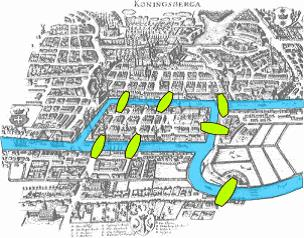
\includegraphics[width=0.8\columnwidth]{bridge.jpg}\\
Image source:\\
\url{http://en.wikipedia.org/wiki/File:Konigsberg_bridges.png}.\\
Used under the license given there
\end{tiny}
\end{spacing}
\end{center}
\end{column}
\begin{column}{0.5\textwidth}
\begin{center}
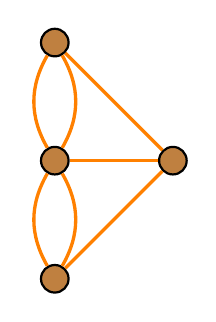
\begin{tikzpicture}[thick,every node/.style={inner sep=0pt,minimum size=3.5mm}]
\node (a) at (0,0) [circle,draw=black,fill=brown]{};
\node (b) at (0,1.5) [circle,draw=black,fill=brown]{};
\node (c) at (0,3) [circle,draw=black,fill=brown]{};
\node (d) at (1.5,1.5) [circle,draw=black,fill=brown]{};
\draw[-,orange,very thick] (c) to [bend left] (b);
\draw[-,orange,very thick] (c) to [bend right] (b);
\draw[-,orange,very thick] (b) to [bend left] (a);
\draw[-,orange,very thick] (b) to [bend right] (a);
\draw[-,orange,very thick] (c) to (d);
\draw[-,orange,very thick] (b) to (d);
\draw[-,orange,very thick] (a) to (d);
\end{tikzpicture}
\end{center}
\end{column}
\end{columns}
\end{DEFINITION}
\end{spacing}
\newpage
\begin{spacing}{1.15}
\begin{THEOREM}
A finite connected multigraph with at least two vertices
has an Euler circuit if and only if each of its vertices has even degree.\\[6pt]
\end{THEOREM}
\begin{PROOF}
\begin{itemize}
  \item[($\Rightarrow$)] Suppose that the multigraph has an Euler circuit starting at some vertex $v_1$. We then ``follow'' the Euler circuit and count 1 degree whenever we ``enter'' a vertex and 1 more degree when we ``leave'' each vertex. We count one degree for v1 as we start by leaving $v_1$. Entering some other vertex, we count 1 as we enter and 1 as we leave. Hence, by traversing the edges of the graph along the circuit, we count two degrees whenever we pass through a vertex. Finally, we ``enter'' the vertex $v_1$ at the final edge of the circuit, counting another degree. Therefore, each vertex of the graph must have an even degree.
\newpage
  \item[($\Leftarrow$)] Suppose the multigraph $G$ is connected and that every vertex has an
even degree. We choose some vertex $v_0$ and arbitrarily choose an
edge $\{v_0, v_1\}$. This is possible, because the graph is connected and
has at least two vertices. We then choose an edge incident to $v_1$,
which is also incident to some vertex $v_2$. We continue to choose
edges in this way until we reach a vertex $v_n$ which has no more edges
incident to it that we have not yet used in our path.\\[6pt]
This will occur because $G$ is assumed to be finite and hence contains
only a finite number of edges.\\[6pt]
We now claim that $v_n = v_0$: The path ``uses'' one degree of each
vertex to enter and one degree to ``leave'' each vertex. Since every
vertex has an even degree, for every edge that is used to ``enter'' the
vertex, there exists exactly one edge to ``leave'' the vertex. Therefore,
if the path arrives at a vertex that can not be ``left'' by an unused
edge, it must be $v_0$.
\newpage
We have now constructed a circuit in the graph $G$. However, it may
not be an Euler circuit, because it might not include every edge in $G$.
Let $H$ be the subgraph of $G$ that contains the edges not already used.
Then we have an Euler circuit of $H\setminus G$. Let $w_0$ be a vertex in $H$ that
is connected to a vertex in $G\setminus H$. Such a vertex exists because $G$ is
connected. Repeat the above procedure to find a circuit in $H$ starting
and ending at $w_0$ and then splice this circuit into the circuit of $H\setminus G$.
We then obtain a new (large) circuit in $G$.\\[6pt]
If there remain unused edges, we repeat the above step until no more
edges remain and our circuit becomes an Euler circuit in $G$. Our
procedure terminates because the graph $G$ is finite.
\end{itemize}
\end{PROOF}
The construction of an Euler circuit can be made into a workable
algorithm. We also note that every circuit is of course a path, so the
existence of an Euler circuit implies the existence of an Euler path.
\newpage
\begin{THEOREM}
A finite connected multigraph has an Euler path but not
an Euler circuit if and only if it has exactly two vertices of odd degree.\\[5pt]
\end{THEOREM}
\begin{PROOF}
\begin{itemize}
  \item[($\Rightarrow$)] Suppose that the multigraph has an Euler path starting at some vertex $v_1$ and ending at some vertex $v_n$. Then the vertex $v_1$ must have odd degree, because it is left once more than it is entered. A similar statement applies to $v_n$. All other vertices are entered and then left an equal number of times. Thus, $v_1$ and $v_n$ have odd degree while all other vertices have even degree.
  \item[($\Leftarrow$)] Suppose that the multigraph $G$ has two vertices, $v_1$ and $v_n$, of odd degree and that all other vertices have even degree. Add an edge $\{v_1, v_n\}$ to $G$. Then every vertex in $G$ has even degree and there exists an Euler circuit starting at $v_1$ and ending at $v_n$. Removing the edge $\{v_1, v_n\}$ from the Euler circuit produces the desired Euler path. (Why exactly?)
\end{itemize}
\end{PROOF}
\end{spacing}
\end{frame}
\begin{frame}[c,allowdisplaybreaks,allowframebreaks]{Hamilton Paths and Circuits}
\begin{spacing}{1.1}
\vspace*{6pt}
\begin{DEFINITION}
Let $G$ be a finite graph.
\begin{itemize}
  \item[1.] A \emph{Hamilton path} in $G$ is a simple path that passes through every vertex of $G$ exactly once.
  \item[2.] A \emph{Hamilton circuit} in $G$ is a simple path that passes through every vertex of $G$ exactly once.
\end{itemize}
There are no known useful necessary and sufficient conditions for the
existence of Hamilton circuits, but there are a few giving sufficient
conditions:\\[5pt]
\stepcounter{zhuo}
\alert{3.2.12. Dirac's Theorem.} Let $G$ be a simple graph with $n\geq 3$ vertices such
that the degree of each vertex is at least $n/2$. Then $G$ has a Hamilton
circuit.\\[5pt]
\alert{3.2.13. Ore's Theorem.} Let $G$ be a simple graph with $n \geq 3$ vertices such that the sum of the degree of any two non-adjacent vertices is at least $n$.
Then $G$ has a Hamilton circuit.
\end{DEFINITION}
\newpage
Clearly, Dirac's Theorem is a Corollary of Ore's Theorem. Ore's Theorem
will be proven in the exercises.\\[6pt]
Hamiltonian circuits appear in many applications. A famous problem that
we will look at later is the \emph{traveling salesman problem}, which asks for the
perfect route a traveling salesman should take to visit a set of cities.
\end{spacing}
\end{frame}
\begin{frame}[t,allowdisplaybreaks,allowframebreaks]{The Icosian Game}
\begin{spacing}{1.05}
William Hamilton studied such paths and circuits and their symmetry
properties. Out of his research he developed a game called the Icosian
game or ``A Voyage Round the World'' which challenges a person to
connect pegs on the edges of a dodecahedron using a string in such a way that all pegs are touched exactly once by the string.\\[3pt]
\begin{columns}[onlytextwidth]
\begin{column}{0.5\textwidth}
\begin{center}
\begin{spacing}{0.5}
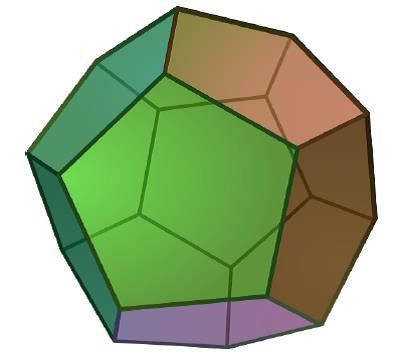
\includegraphics[width=0.7\columnwidth,height=120pt]{pent.jpg}\\
\begin{tiny}
Image source:\\
\url{http://commons.wikimedia.org/wiki/File:}\\
POV-Ray-Dodecahedron.svg\\
Used under the license given there
\end{tiny}
\end{spacing}
\end{center}
\end{column}
\begin{column}{0.5\textwidth}
\begin{center}
\begin{spacing}{0.5}
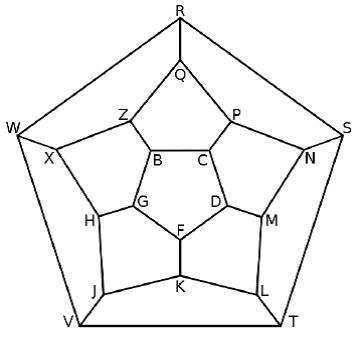
\includegraphics[width=0.7\columnwidth,height=100pt]{pent2.jpg}\\
\begin{tiny}
Image source:\\
\url{http://commons.wikimedia.org/wiki/File:}\\
Icosian\_grid\_small\_with\_labels.svg\\
Used under the license given there
\end{tiny}
\end{spacing}
\end{center}
\end{column}
\end{columns}
\newpage
A solution is shown below:\\
\begin{center}
\begin{spacing}{0.5}
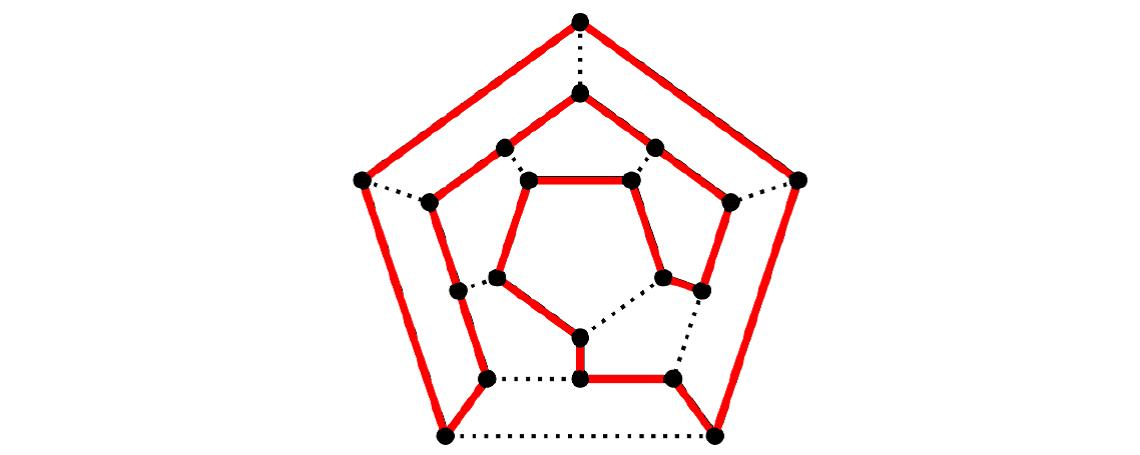
\includegraphics[width=\textwidth,height=110pt]{pent3.jpg}
\begin{tiny}
Image source:\\
\url{http://commons.wikimedia.org/wiki/File:Hamiltonian\_path.svg}\\
Used under the license given there
\end{tiny}
\end{spacing}
\end{center}
A three-dimensional image of the solution can be found at \url{http://mathworld.wolfram.com/IcosianGame.html}
\end{spacing}
\end{frame}
\begin{frame}[t]{Weighted Graphs}
\begin{spacing}{0.95}
\vspace*{-7pt}
A weighted graph is a graph where each edge is assigned a weight. For
example, the image below gives the distances (in miles) between various
cities in the United States:\\
\begin{center}
\begin{spacing}{0.5}
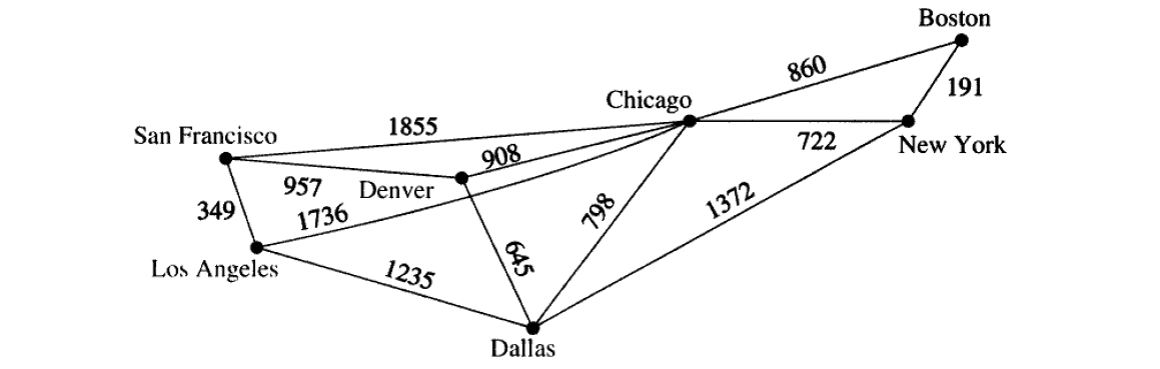
\includegraphics[width=\textwidth,height=110pt]{route}
\begin{tiny}
Image source: Rosen, K.H., \emph{Discrete Mathematics}, 6\textsuperscript{th} Ed., McGraw-Hill International Edition 2007\\
Used under fair use exemption.
\end{tiny}
\end{spacing}
\end{center}
\vspace*{-6pt}
We are interested in paths in weighted graphs. The \emph{length} of a path in a
weighted graph is given by the sum of the weights of the edges comprising
the path. An empty path consisting of no edges is said to have length
infinity.
\end{spacing}
\end{frame}
\begin{frame}[t]{Shortest Paths in Weighted Graphs}
\begin{spacing}{0.9}
Suppose we are given an undirected, connected, simple, weighted path. Given two vertices $a$ and $z$, our goal is to find the shortest path (i.e., the path of least length) that joins $a$ to $z$. We will here present an algorithm due to Dijkstra that finds this shortest path.\\[6pt]
The algorithm proceeds in several iterations. In the $k$th iteration, we will form a distinguished set of vertices, called $S_k$. Furthermore, in each iteration we will assign the labels $L_k(v)$ to the vertex $v$.\\[6pt]
We start with the $k=0$th iteration, setting
\[S_0:=\emptyset,\qquad\qquad\qquad
L_0(v)=\begin{cases}
         0, & v=a, \\
         \infty, & v\neq a.
       \end{cases}\]
We find $S_{k+1}$ from $S_k,\,k\in\N$, by adding a vertex $u$ to $S_k$ with the smallest label. Then, we update the labels of all vertices not in $S_{k+1}$ so that
\begin{equation}\label{3.2.2}
L_{k+1}(v)=\min\big\{L_k(v),L_k(u)+w(u,v)\big\}
\end{equation}
where $w(u,v)$ denotes the weight of the edge $\{u,v\}$.
\end{spacing}
\end{frame}
\begin{frame}[t]{Dijkstra's Algorithm}
\begin{spacing}{0.9}
We claim that
\begin{equation*}
  \begin{split}
     L_k(v)= &\text{length of the shortest path from $a$ to $v$} \\
       &\text{that contains only vertices in $S_k$}.
  \end{split}
\end{equation*}
Once $z$ is added to $S_k$, the length of the shortest path is given by the label of $z$.\\[5pt]
\begin{EXAMPLE}
We will find the shortest path from $a$ to $z$ in the graph given below:\\
\begin{center}
\tikzset{
my state/.style={circle,draw,thick,inner sep=0pt,minimum size=5.5mm},
my state2/.style={circle,inner sep=0pt,minimum size=5mm}}
\begin{tikzpicture}[line width=0.4mm,node distance=2cm,on grid,
every state/.style={draw=black,fill=white,text=black,very thick}]
\node[my state] (a) at (0,0) {$a$};
\node[my state] (b) at (1.5,1.5) {$b$};
 \node[my state] (c) at (1.5,-1.5) {$c$};
 \node[my state] (d) at (4.5,1.5) {$d$};
 \node[my state] (e) at (4.5,-1.5) {$e$};
 \node[my state] (z) at (6,0) {$z$};
 \node[my state2] (4) at (0.75,0.75) {$4$};
 \node[my state2] (2) at (0.75,-0.75) {$2$};
 \node[my state2] (5) at (3,1.5) {$5$};
 \node[my state2] (1) at (1.5,0) {$1$};
 \node[my state2] (3) at (5.25,-0.75) {$3$};
 \node[my state2] (6) at (5.25,0.75) {$6$};
 \node[my state2] (22) at (4.5,0) {$2$};
 \node[my state2] (8) at (3,0) {$8$};
 \node[my state2] (10) at (3,-1.5) {$10$};
 \draw (a) -- (4);
 \draw (4) -- (b);
 \draw (a) -- (2);
 \draw (2) -- (c);
 \draw (b) -- (1);
 \draw (1) -- (c);
 \draw (b) -- (5);
 \draw (5) -- (d);
 \draw (c) -- (8);
 \draw (8) -- (d);
 \draw (c) -- (10);
 \draw (10) -- (e);
 \draw (d) -- (22);
 \draw (22) -- (e);
 \draw (d) -- (6);
 \draw (6) -- (z);
 \draw (e) -- (3);
 \draw (3) -- (z);
\end{tikzpicture}
\end{center}
\end{EXAMPLE}
\end{spacing}
\end{frame}
\begin{frame}[t]{Dijkstra's Algorithm - 0\textsuperscript{th} Iteration}
$S_0=\emptyset$.\\[6pt]
\tikzset{
my state/.style={circle,draw,thick,inner sep=0pt,minimum size=5.5mm},
my state2/.style={circle,inner sep=0pt,minimum size=5mm}}
\begin{tikzpicture}[line width=0.4mm,node distance=2cm,on grid,
every state/.style={draw=black,fill=white,text=black,very thick}]
\node[my state] (a) at (0,0) {$a$};
\node[my state] (b) at (2,2) {$b$};
 \node[my state] (c) at (2,-2) {$c$};
 \node[my state] (d) at (6,2) {$d$};
 \node[my state] (e) at (6,-2) {$e$};
 \node[my state] (z) at (8,0) {$z$};
 \node[my state2] (4) at (1,1) {$4$};
 \node[my state2] (2) at (1,-1) {$2$};
 \node[my state2] (5) at (4,2) {$5$};
 \node[my state2] (1) at (2,0) {$1$};
 \node[my state2] (3) at (7,-1) {$3$};
 \node[my state2] (6) at (7,1) {$6$};
 \node[my state2] (22) at (6,0) {$2$};
 \node[my state2] (8) at (4,0) {$8$};
 \node[my state2] (10) at (4,-2) {$10$};
 \draw (a) -- (4);
 \draw (4) -- (b);
 \draw (a) -- (2);
 \draw (2) -- (c);
 \draw (b) -- (1);
 \draw (1) -- (c);
 \draw (b) -- (5);
 \draw (5) -- (d);
 \draw (c) -- (8);
 \draw (8) -- (d);
 \draw (c) -- (10);
 \draw (10) -- (e);
 \draw (d) -- (22);
 \draw (22) -- (e);
 \draw (d) -- (6);
 \draw (6) -- (z);
 \draw (e) -- (3);
 \draw (3) -- (z);
 \node [left=0.4cm] at (a) {\textcolor[rgb]{1.00,0.30,0.00}{0}};
 \node [above=0.4cm] at (b) {\textcolor[rgb]{1.00,0.30,0.00}{$\infty$}};
 \node [below=0.4cm] at (c) {\textcolor[rgb]{1.00,0.30,0.00}{$\infty$}};
 \node [above=0.4cm] at (d) {\textcolor[rgb]{1.00,0.30,0.00}{$\infty$}};
 \node [below=0.4cm] at (e) {\textcolor[rgb]{1.00,0.30,0.00}{$\infty$}};
 \node [right=0.4cm] at (z) {\textcolor[rgb]{1.00,0.30,0.00}{$\infty$}};
\end{tikzpicture}
\end{frame}
\begin{frame}[t]{Dijkstra's Algorithm - 1\textsuperscript{st} Iteration}
$S_1=\{a\}$.\\[6pt]
\tikzset{
my state/.style={circle,draw,thick,inner sep=0pt,minimum size=5.5mm},
my state2/.style={circle,inner sep=0pt,minimum size=5mm}}
\begin{tikzpicture}[line width=0.4mm,node distance=2cm,on grid,
every state/.style={draw=black,fill=white,text=black,very thick}]
\node[my state,fill=orange] (a) at (0,0) {$a$};
\node[my state] (b) at (2,2) {$b$};
 \node[my state] (c) at (2,-2) {$c$};
 \node[my state] (d) at (6,2) {$d$};
 \node[my state] (e) at (6,-2) {$e$};
 \node[my state] (z) at (8,0) {$z$};
 \node[my state2] (4) at (1,1) {$4$};
 \node[my state2] (2) at (1,-1) {$2$};
 \node[my state2] (5) at (4,2) {$5$};
 \node[my state2] (1) at (2,0) {$1$};
 \node[my state2] (3) at (7,-1) {$3$};
 \node[my state2] (6) at (7,1) {$6$};
 \node[my state2] (22) at (6,0) {$2$};
 \node[my state2] (8) at (4,0) {$8$};
 \node[my state2] (10) at (4,-2) {$10$};
 \draw (a) -- (4);
 \draw (4) -- (b);
 \draw (a) -- (2);
 \draw (2) -- (c);
 \draw (b) -- (1);
 \draw (1) -- (c);
 \draw (b) -- (5);
 \draw (5) -- (d);
 \draw (c) -- (8);
 \draw (8) -- (d);
 \draw (c) -- (10);
 \draw (10) -- (e);
 \draw (d) -- (22);
 \draw (22) -- (e);
 \draw (d) -- (6);
 \draw (6) -- (z);
 \draw (e) -- (3);
 \draw (3) -- (z);
 \node [left=0.4cm] at (a) {\textcolor[rgb]{1.00,0.30,0.00}{0}};
 \node [above=0.4cm] at (b) {\textcolor[rgb]{1.00,0.30,0.00}{$4(a)$}};
 \node [below=0.4cm] at (c) {\textcolor[rgb]{1.00,0.30,0.00}{$2(a)$}};
 \node [above=0.4cm] at (d) {\textcolor[rgb]{1.00,0.30,0.00}{$\infty$}};
 \node [below=0.4cm] at (e) {\textcolor[rgb]{1.00,0.30,0.00}{$\infty$}};
 \node [right=0.4cm] at (z) {\textcolor[rgb]{1.00,0.30,0.00}{$\infty$}};
\end{tikzpicture}
\end{frame}
\begin{frame}[t]{Dijkstra's Algorithm - 2\textsuperscript{nd} Iteration}
$S_2=\{a,c\}$.\\[6pt]
\tikzset{
my state/.style={circle,draw,thick,inner sep=0pt,minimum size=5.5mm},
my state2/.style={circle,inner sep=0pt,minimum size=5mm}}
\begin{tikzpicture}[line width=0.4mm,node distance=2cm,on grid,
every state/.style={draw=black,fill=white,text=black,very thick}]
\node[my state,fill=orange] (a) at (0,0) {$a$};
\node[my state] (b) at (2,2) {$b$};
 \node[my state,fill=orange] (c) at (2,-2) {$c$};
 \node[my state] (d) at (6,2) {$d$};
 \node[my state] (e) at (6,-2) {$e$};
 \node[my state] (z) at (8,0) {$z$};
 \node[my state2] (4) at (1,1) {$4$};
 \node[my state2] (2) at (1,-1) {$2$};
 \node[my state2] (5) at (4,2) {$5$};
 \node[my state2] (1) at (2,0) {$1$};
 \node[my state2] (3) at (7,-1) {$3$};
 \node[my state2] (6) at (7,1) {$6$};
 \node[my state2] (22) at (6,0) {$2$};
 \node[my state2] (8) at (4,0) {$8$};
 \node[my state2] (10) at (4,-2) {$10$};
 \draw (a) -- (4);
 \draw (4) -- (b);
 \draw (a) -- (2);
 \draw (2) -- (c);
 \draw (b) -- (1);
 \draw (1) -- (c);
 \draw (b) -- (5);
 \draw (5) -- (d);
 \draw (c) -- (8);
 \draw (8) -- (d);
 \draw (c) -- (10);
 \draw (10) -- (e);
 \draw (d) -- (22);
 \draw (22) -- (e);
 \draw (d) -- (6);
 \draw (6) -- (z);
 \draw (e) -- (3);
 \draw (3) -- (z);
 \node [left=0.4cm] at (a) {\textcolor[rgb]{1.00,0.30,0.00}{0}};
 \node [above=0.4cm] at (b) {\textcolor[rgb]{1.00,0.30,0.00}{$3(a,c)$}};
 \node [below=0.4cm] at (c) {\textcolor[rgb]{1.00,0.30,0.00}{$2(a)$}};
 \node [above=0.4cm] at (d) {\textcolor[rgb]{1.00,0.30,0.00}{$10(a,c)$}};
 \node [below=0.4cm] at (e) {\textcolor[rgb]{1.00,0.30,0.00}{$12(a,c)$}};
 \node [right=0.4cm] at (z) {\textcolor[rgb]{1.00,0.30,0.00}{$\infty$}};
\end{tikzpicture}
\end{frame}
\begin{frame}[t]{Dijkstra's Algorithm - 3\textsuperscript{rd} Iteration}
$S_3=\{a,b,c\}$.\\[6pt]
\tikzset{
my state/.style={circle,draw,thick,inner sep=0pt,minimum size=5.5mm},
my state2/.style={circle,inner sep=0pt,minimum size=5mm}}
\begin{tikzpicture}[line width=0.4mm,node distance=2cm,on grid,
every state/.style={draw=black,fill=white,text=black,very thick}]
\node[my state,fill=orange] (a) at (0,0) {$a$};
\node[my state,fill=orange] (b) at (2,2) {$b$};
 \node[my state,fill=orange] (c) at (2,-2) {$c$};
 \node[my state] (d) at (6,2) {$d$};
 \node[my state] (e) at (6,-2) {$e$};
 \node[my state] (z) at (8,0) {$z$};
 \node[my state2] (4) at (1,1) {$4$};
 \node[my state2] (2) at (1,-1) {$2$};
 \node[my state2] (5) at (4,2) {$5$};
 \node[my state2] (1) at (2,0) {$1$};
 \node[my state2] (3) at (7,-1) {$3$};
 \node[my state2] (6) at (7,1) {$6$};
 \node[my state2] (22) at (6,0) {$2$};
 \node[my state2] (8) at (4,0) {$8$};
 \node[my state2] (10) at (4,-2) {$10$};
 \draw (a) -- (4);
 \draw (4) -- (b);
 \draw (a) -- (2);
 \draw (2) -- (c);
 \draw (b) -- (1);
 \draw (1) -- (c);
 \draw (b) -- (5);
 \draw (5) -- (d);
 \draw (c) -- (8);
 \draw (8) -- (d);
 \draw (c) -- (10);
 \draw (10) -- (e);
 \draw (d) -- (22);
 \draw (22) -- (e);
 \draw (d) -- (6);
 \draw (6) -- (z);
 \draw (e) -- (3);
 \draw (3) -- (z);
 \node [left=0.4cm] at (a) {\textcolor[rgb]{1.00,0.30,0.00}{0}};
 \node [above=0.4cm] at (b) {\textcolor[rgb]{1.00,0.30,0.00}{$3(a,c)$}};
 \node [below=0.4cm] at (c) {\textcolor[rgb]{1.00,0.30,0.00}{$2(a)$}};
 \node [above=0.4cm] at (d) {\textcolor[rgb]{1.00,0.30,0.00}{$8(a,c,b)$}};
 \node [below=0.4cm] at (e) {\textcolor[rgb]{1.00,0.30,0.00}{$12(a,c)$}};
 \node [right=0.4cm] at (z) {\textcolor[rgb]{1.00,0.30,0.00}{$\infty$}};
\end{tikzpicture}
\end{frame}
\begin{frame}[t]{Dijkstra's Algorithm - 4\textsuperscript{th} Iteration}
$S_4=\{a,b,c,d\}$.\\[6pt]
\tikzset{
my state/.style={circle,draw,thick,inner sep=0pt,minimum size=5.5mm},
my state2/.style={circle,inner sep=0pt,minimum size=5mm}}
\begin{tikzpicture}[line width=0.4mm,node distance=2cm,on grid,
every state/.style={draw=black,fill=white,text=black,very thick}]
\node[my state,fill=orange] (a) at (0,0) {$a$};
\node[my state,fill=orange] (b) at (2,2) {$b$};
 \node[my state,fill=orange] (c) at (2,-2) {$c$};
 \node[my state,fill=orange] (d) at (6,2) {$d$};
 \node[my state] (e) at (6,-2) {$e$};
 \node[my state] (z) at (8,0) {$z$};
 \node[my state2] (4) at (1,1) {$4$};
 \node[my state2] (2) at (1,-1) {$2$};
 \node[my state2] (5) at (4,2) {$5$};
 \node[my state2] (1) at (2,0) {$1$};
 \node[my state2] (3) at (7,-1) {$3$};
 \node[my state2] (6) at (7,1) {$6$};
 \node[my state2] (22) at (6,0) {$2$};
 \node[my state2] (8) at (4,0) {$8$};
 \node[my state2] (10) at (4,-2) {$10$};
 \draw (a) -- (4);
 \draw (4) -- (b);
 \draw (a) -- (2);
 \draw (2) -- (c);
 \draw (b) -- (1);
 \draw (1) -- (c);
 \draw (b) -- (5);
 \draw (5) -- (d);
 \draw (c) -- (8);
 \draw (8) -- (d);
 \draw (c) -- (10);
 \draw (10) -- (e);
 \draw (d) -- (22);
 \draw (22) -- (e);
 \draw (d) -- (6);
 \draw (6) -- (z);
 \draw (e) -- (3);
 \draw (3) -- (z);
 \node [left=0.4cm] at (a) {\textcolor[rgb]{1.00,0.30,0.00}{0}};
 \node [above=0.4cm] at (b) {\textcolor[rgb]{1.00,0.30,0.00}{$3(a,c)$}};
 \node [below=0.4cm] at (c) {\textcolor[rgb]{1.00,0.30,0.00}{$2(a)$}};
 \node [above=0.4cm] at (d) {\textcolor[rgb]{1.00,0.30,0.00}{$8(a,c,b)$}};
 \node [below=0.4cm] at (e) {\textcolor[rgb]{1.00,0.30,0.00}{$10(a,c,b,d)$}};
 \node [right=0.4cm] at (z) {\textcolor[rgb]{1.00,0.30,0.00}{$14(a,c,b,d)$}};
\end{tikzpicture}
\end{frame}
\begin{frame}[t]{Dijkstra's Algorithm - 5\textsuperscript{th} Iteration}
$S_5=\{a,b,c,d,e\}$.\\[6pt]
\tikzset{
my state/.style={circle,draw,thick,inner sep=0pt,minimum size=5.5mm},
my state2/.style={circle,inner sep=0pt,minimum size=5mm}}
\begin{tikzpicture}[line width=0.4mm,node distance=2cm,on grid,
every state/.style={draw=black,fill=white,text=black,very thick}]
\node[my state,fill=orange] (a) at (0,0) {$a$};
\node[my state,fill=orange] (b) at (2,2) {$b$};
 \node[my state,fill=orange] (c) at (2,-2) {$c$};
 \node[my state,fill=orange] (d) at (6,2) {$d$};
 \node[my state,fill=orange] (e) at (6,-2) {$e$};
 \node[my state] (z) at (8,0) {$z$};
 \node[my state2] (4) at (1,1) {$4$};
 \node[my state2] (2) at (1,-1) {$2$};
 \node[my state2] (5) at (4,2) {$5$};
 \node[my state2] (1) at (2,0) {$1$};
 \node[my state2] (3) at (7,-1) {$3$};
 \node[my state2] (6) at (7,1) {$6$};
 \node[my state2] (22) at (6,0) {$2$};
 \node[my state2] (8) at (4,0) {$8$};
 \node[my state2] (10) at (4,-2) {$10$};
 \draw (a) -- (4);
 \draw (4) -- (b);
 \draw (a) -- (2);
 \draw (2) -- (c);
 \draw (b) -- (1);
 \draw (1) -- (c);
 \draw (b) -- (5);
 \draw (5) -- (d);
 \draw (c) -- (8);
 \draw (8) -- (d);
 \draw (c) -- (10);
 \draw (10) -- (e);
 \draw (d) -- (22);
 \draw (22) -- (e);
 \draw (d) -- (6);
 \draw (6) -- (z);
 \draw (e) -- (3);
 \draw (3) -- (z);
 \node [left=0.4cm] at (a) {\textcolor[rgb]{1.00,0.30,0.00}{0}};
 \node [above=0.4cm] at (b) {\textcolor[rgb]{1.00,0.30,0.00}{$3(a,c)$}};
 \node [below=0.4cm] at (c) {\textcolor[rgb]{1.00,0.30,0.00}{$2(a)$}};
 \node [above=0.4cm] at (d) {\textcolor[rgb]{1.00,0.30,0.00}{$8(a,c,b)$}};
 \node [below=0.4cm] at (e) {\textcolor[rgb]{1.00,0.30,0.00}{$10(a,c,b,d)$}};
 \node [right=0.4cm] at (z) {\textcolor[rgb]{1.00,0.30,0.00}{$13(a,c,b,d,e)$}};
\end{tikzpicture}
\end{frame}
\begin{frame}[t]{Dijkstra's Algorithm - 6\textsuperscript{th} Iteration}
$S_6=\{a,b,c,d,e,z\}$.\\[6pt]
\tikzset{
my state/.style={circle,draw,thick,inner sep=0pt,minimum size=5.5mm},
my state2/.style={circle,inner sep=0pt,minimum size=5mm}}
\begin{tikzpicture}[line width=0.4mm,node distance=2cm,on grid,
every state/.style={draw=black,fill=white,text=black,very thick}]
\node[my state,fill=orange] (a) at (0,0) {$a$};
\node[my state,fill=orange] (b) at (2,2) {$b$};
 \node[my state,fill=orange] (c) at (2,-2) {$c$};
 \node[my state,fill=orange] (d) at (6,2) {$d$};
 \node[my state,fill=orange] (e) at (6,-2) {$e$};
 \node[my state,fill=orange] (z) at (8,0) {$z$};
 \node[my state2] (4) at (1,1) {$4$};
 \node[my state2] (2) at (1,-1) {$2$};
 \node[my state2] (5) at (4,2) {$5$};
 \node[my state2] (1) at (2,0) {$1$};
 \node[my state2] (3) at (7,-1) {$3$};
 \node[my state2] (6) at (7,1) {$6$};
 \node[my state2] (22) at (6,0) {$2$};
 \node[my state2] (8) at (4,0) {$8$};
 \node[my state2] (10) at (4,-2) {$10$};
 \draw (a) -- (4);
 \draw (4) -- (b);
 \draw (a) -- (2);
 \draw (2) -- (c);
 \draw (b) -- (1);
 \draw (1) -- (c);
 \draw (b) -- (5);
 \draw (5) -- (d);
 \draw (c) -- (8);
 \draw (8) -- (d);
 \draw (c) -- (10);
 \draw (10) -- (e);
 \draw (d) -- (22);
 \draw (22) -- (e);
 \draw (d) -- (6);
 \draw (6) -- (z);
 \draw (e) -- (3);
 \draw (3) -- (z);
 \node [left=0.4cm] at (a) {\textcolor[rgb]{1.00,0.30,0.00}{0}};
 \node [above=0.4cm] at (b) {\textcolor[rgb]{1.00,0.30,0.00}{$3(a,c)$}};
 \node [below=0.4cm] at (c) {\textcolor[rgb]{1.00,0.30,0.00}{$2(a)$}};
 \node [above=0.4cm] at (d) {\textcolor[rgb]{1.00,0.30,0.00}{$8(a,c,b)$}};
 \node [below=0.4cm] at (e) {\textcolor[rgb]{1.00,0.30,0.00}{$10(a,c,b,d)$}};
 \node [right=0.4cm] at (z) {\textcolor[rgb]{1.00,0.30,0.00}{$13(a,c,b,d,e)$}};
\end{tikzpicture}
\end{frame}
\begin{frame}[t,allowdisplaybreaks,allowframebreaks]{Dijkstra's Algorithm}
\begin{spacing}{1.15}
To establish that Dijkstra's algorithm actually gives shortest path from $a$
to $z$, we will prove the following result:\\[5pt]
\begin{THEOREM}
Let $G$ be an undirected, weighted, connected graph and $a$ a vertex in $G$. At the $k$th iteration of Dijkstra's algorithm,
\begin{itemize}
  \item[(i)] The label $L_k(v)$ of every vertex $v\in S_k$ is the length of a shortest path from $a$ to $v$;
  \item[(ii)] The label $L_k(w)$ of every vertex $w\notin S_k$ is the length of a shortest path from $a$ to $w$ that contains only (besides $w$ itself) vertices in $S_k$.
\end{itemize}
\begin{PROOF}
We prove these statements by induction in $k\in\N$. For $k=0,\,S_0=\emptyset$, so (i) is vacuously true. Furthermore, there is no path from a to a vertex
other than a using vertices in $S_0$, so, by definition, its length is $\infty$. It follows that (i) and (ii) are true for $k=0$.
\newpage
\alert{Proof (continued).}\\
Assume that (i) and (ii) are true for $k\in\N$. The vertices in $S_k$ are hence labeled with the length of the shortest path from $a$. Let $u \in S_{k+1}$ but
$u\notin
S_k$, so $u$ is the vertex added in the $k$th iteration. Thus, $u$ has a
smallest label of all vertices not in $S_k$.\\[6pt]
It is clear (from (ii)) that $u$ is labeled with the length of a shortest path
containing only vertices in $S_k$. We claim that the label of $u$ is actually the length of a shortest path without regard to where the path's vertices lie. We show this by contradiction: Suppose that there exists a path of length less than $L_k (u)$ from $a$ to $u$ containing a vertex not in $S_k$. Let $v$ be the first vertex along this path which is not in $S_k$. Then $L_k(v) < L_k (u)$ so $v$
should have been added to $S_k$ instead of $u$, giving a contradiction. Hence
the label of $u$ is the shortest path from $a$ to $u$. This implies (i) with $k$
replaced by $k + 1$.
\newpage
\alert{Proof (continued).}\\
Let $v\notin S_{k+1}$. A shortest path from $a$ to $v$ containing only elements of
$S_{k+1}$ either contains $u$ or it does not. If it does not contain $u$, then
$L_{k+1}(v) = L_k (v)$ is the length of the shortest path from $a$ to $v$ since we assumed that (ii) is true for $k$. If it does contain $u$, the path is made up of
a shortest path from $a$ to $u$ followed by the edge from $u$ to $v$. (Why?) But
then the length of this path is just given by the right-hand side of \eqref{3.2.2}
which is equal to the label $L_{k+1}(v)$. Thus, (ii) is true with $k$ replaced by $k + 1$.
\end{PROOF}
\vspace*{6pt}
\begin{COROLLARY}
Dijktsra's algorithm finds the length of a shortest path
between two vertices in a connected simple undirected weighted graph.\\[6pt]
\end{COROLLARY}
\begin{THEOREM}
Dijkstra's algorithm uses $O(n^2)$ operations (additions
and comparisons) to find the length of a shortest path between two vertices in a connected simple undirected weighted graph consisting of $n$ vertices.
\end{THEOREM}
\end{THEOREM}
\end{spacing}
\end{frame}
\begin{frame}[t,allowdisplaybreaks,allowframebreaks]{The Traveling Salesman Problem}
\begin{spacing}{1.1}
Consider the following problem: a traveling salesman needs to visit the
cities Detroit, Toledo, Grand Rapids, Saginaw and Kalamazoo, shown in
the graph below with the distances from each other:
\begin{center}
\tikzset{
my state/.style={circle,draw,thick,inner sep=0pt,minimum size=4.5mm,fill=blue},
my state2/.style={circle,draw=white,fill=white,inner sep=0pt,minimum size=5mm}}
\begin{tikzpicture}[node distance=2cm,on grid,
every state/.style={draw=black,fill=white,text=black,very thick},line width=0.3mm]
\node[my state] (C) at (0,1.2) {};
\node[my state] (D) at (0,-1.2) {};
 \node[my state] (B) at (2.28254,1.94164) {};
 \node[my state] (E) at (2.28254,-1.94164) {};
 \node[my state] (A) at (3.69320,0) {};
 \node [right=0.2cm] at (A) {Detroit};
 \node [above left=0.2cm] at (C) {Grand Rapids};
 \node [above right=0.2cm] at (B) {Saginaw};
 \node [below left=0.2cm] at (D) {Kalamazoo};
 \node [below right=0.2cm] at (E) {Toledo};
 \node[my state2] (CB) at (1.14127,1.57082) {113};
 \node[my state2] (CD) at (0,0) {56};
 \node[my state2] (DE) at (1.14127,-1.57082) {133};
 \node[my state2] (AB) at (2.99,0.97) {98};
 \node[my state2] (AE) at (2.99,-0.97) {58};
 \node[my state2] (AC) at (1.8466,0.6) {147};
 \node[my state2] (AD) at (1.8466,-0.6) {135};
 \node[my state2] (BD) at (1.14127,0.37082) {137};
 \node[my state2] (CE) at (1.14127,-0.37082) {167};
 \node[my state2] (BE) at (2.28254,0) {142};
 \draw[-] (C) to (CB);
 \draw[-] (B) to (CB);
 \draw[-] (B) to (AB);
 \draw[-] (A) to (AB);
 \draw[-] (A) to (AE);
 \draw[-] (E) to (AE);
 \draw[-] (D) to (DE);
 \draw[-] (E) to (DE);
 \draw[-] (C) to (CD);
 \draw[-] (D) to (CD);
 \draw[-] (B) to (BD);
 \draw[-] (D) to (BD);
 \draw[-] (B) to (BE);
 \draw[-] (E) to (BE);
 \draw[-] (A) to (AC);
 \draw[-] (C) to (AC);
 \draw[-] (A) to (AD);
 \draw[-] (D) to (AD);
 \draw[-] (C) to (CE);
 \draw[-] (E) to (CE);
\end{tikzpicture}
\end{center}
\newpage
\vspace*{6pt}
The traveling salesman problem asks: in which order should the cities be
visited to minimize the total distance travelled, assuming that he starts
and ends his tour in Detroit? In other words, we are looking for the
shortest Hamilton circuit of the graph starting and ending in Detroit. In
our example, the graph is complete, so we can visit the cities in any order.
By checking each possible route individually, it turns out that the circuit
\[\text{Detroit - Grand Rapids - Toledo - Saginaw - Kalamazoo - Detroit}\]
is longest, taking 728 miles, while
\[\text{Detroit - Toledo - Kalamazoo - Grand Rapids - Saginaw - Detroit}\]
is shortest with a length of 458 miles.
\newpage
\vspace*{9pt}
To solve the traveling salesman problem naively in a graph with $n$ vertices,
one must examine $(n-1)!/2=O(n!)$ different Hamilton circuits – a
prohibitive task for any realistic $n$. Due to the great practical importance
of the problem, more efficient algorithms have been developed. These,
however, are all exponential in time, and in fact, it has been shown that
the problem belongs to the class of NP-complete problems.\\[6pt]
There exist polynomial-time algorithms that do not find the shortest
possible route (of weight $w_{\min}$ but rather a route of weight less than $c\cdot w_{\min}$, for example with $c=3/2$. In practice, there are algorithms that solve the problem in graphs of 1000 vertices within 2\% of the shortest path length in a few minutes of computer time.
\end{spacing}
\end{frame}
\subsection{Planar Graphs}
\begin{frame}[c] \begin{spacing}{2.5}
\tableofcontents[sectionstyle=hide,subsectionstyle=show/shaded/hide] \end{spacing}
\end{frame}
\begin{frame}[t,allowdisplaybreaks,allowframebreaks]{Planar Graphs}
\begin{spacing}{1.05}
\vspace*{6pt}
\begin{DEFINITION}
A graph is said to be \emph{planar} if it can be drawn in the
plane without any edges crossing. Such a drawing is called a \emph{planar
representation} of the graph.\\[6pt]
\end{DEFINITION}
\begin{EXAMPLE}
The complete graph $K_4$ is planar:\\[25pt]
\begin{columns}[onlytextwidth]
\begin{column}{0.3\textwidth}
\begin{center}
\begin{tikzpicture}[thick,every node/.style={inner sep=0pt,minimum size=3.5mm}]
\node (a) at (0,0) [circle,draw=black,fill=brown]{};
\node (b) at (0,2) [circle,draw=black,fill=brown]{};
\node (c) at (2,0) [circle,draw=black,fill=brown]{};
\node (d) at (2,2) [circle,draw=black,fill=brown]{};
\draw[-,orange,very thick] (a) to (b);
\draw[-,orange,very thick] (b) to (d);
\draw[-,orange,very thick] (a) to (d);
\draw[-,orange,very thick] (a) to (c);
\draw[-,orange,very thick] (b) to (c);
\draw[-,orange,very thick] (c) to (d);
\end{tikzpicture}
\end{center}
\end{column}
\begin{column}{0.3\textwidth}
\begin{center}
can be drawn as
\end{center}
\end{column}
\begin{column}{0.3\textwidth}
\begin{tikzpicture}[thick,every node/.style={inner sep=0pt,minimum size=3.5mm}]
\node (a) at (0,0) [circle,draw=black,fill=brown]{};
\node (b) at (1,1) [circle,draw=black,fill=brown]{};
\node (c) at (2,0) [circle,draw=black,fill=brown]{};
\node (d) at (2,2) [circle,draw=black,fill=brown]{};
\draw[-,orange,very thick] (a) to (b);
\draw[-,orange,very thick] (b) to (d);
\draw[-,orange,very thick] (a) [bend left] to (d);
\draw[-,orange,very thick] (a) to (c);
\draw[-,orange,very thick] (b) to (c);
\draw[-,orange,very thick] (c) to (d);
\end{tikzpicture}
\end{column}
\end{columns}
\end{EXAMPLE}
\newpage
\begin{columns}[onlytextwidth]
\begin{column}{0.6\textwidth}
\begin{EXAMPLE}
The complete bipartite graph $K_{3,3}$ (see Example 3.1.23) is shown at right:
\end{EXAMPLE}
\end{column}
\begin{column}{0.4\textwidth}
\begin{center}
\tikzset{
my state/.style={circle,draw,thick,inner sep=0pt,minimum size=7mm}}
\begin{tikzpicture}[node distance=2cm,on grid,
every state/.style={draw=black,fill=white,text=black,very thick}]
\node[my state] (v1) at (0,0) {$v_1$};
 \node[my state] (v2) at (1.5,0) {$v_2$};
 \node[my state] (v3) at (3,0) {$v_3$};
 \node[my state] (v4) at (0,-1.5) {$v_4$};
 \node[my state] (v5) at (1.5,-1.5) {$v_5$};
 \node[my state] (v6) at (3,-1.5) {$v_6$};
 \draw[-] (v1) -- (v4);
 \draw[-] (v1) -- (v5);
 \draw[-] (v1) -- (v6);
 \draw[-] (v2) -- (v4);
 \draw[-] (v2) -- (v5);
 \draw[-] (v2) -- (v6);
 \draw[-] (v3) -- (v4);
 \draw[-] (v3) -- (v5);
 \draw[-] (v3) -- (v6);
\end{tikzpicture}\\[7pt]
\end{center}
\end{column}
\end{columns}
\vspace*{6pt}
We will show that it is non-planar. In any planar representation, the
vertices $v_1$ and $v_2$ are connected to both $v_4$ and $v_5$, splitting the plane into
two regions, $R_1$ and $R_2$:
\begin{center}
\tikzset{
my state/.style={circle,draw,thick,inner sep=0pt,minimum size=6.5mm},
my state2/.style={circle,draw=white, inner sep=0pt,minimum size=5mm}}
\begin{tikzpicture}[node distance=2cm,on grid,
every state/.style={draw=black,fill=white,text=black,very thick}]
\node[my state] (v1) at (0,0) {$v_1$};
 \node[my state] (v2) at (2,-2) {$v_2$};
 \node[my state] (v4) at (0,-2) {$v_4$};
 \node[my state] (v5) at (2,0) {$v_5$};
 \draw[-,very thick] (v1) -- (v4);
 \draw[-,very thick] (v1) -- (v5);
 \draw[-,very thick] (v2) -- (v4);
 \draw[-,very thick] (v2) -- (v5);
 \node[my state2] (R2) at (1,-1) {$R_2$};
 \node[my state2] (R1) at (3,-1) {$R_1$};
\end{tikzpicture}\\[7pt]
\end{center}
\newpage
Now suppose the vertex $v_3$ is in the region $R_2$. The region $R_2$ is then
divided into two subregions, $R_{21}$ and $R_{22}$, as shown below:
\begin{center}
\tikzset{
my state/.style={circle,draw,thick,inner sep=0pt,minimum size=6.5mm},
my state2/.style={circle,draw=white, inner sep=0pt,minimum size=5mm}}
\begin{tikzpicture}[node distance=2cm,on grid,
every state/.style={draw=black,fill=white,text=black,very thick}]
\node[my state] (v1) at (0,0) {$v_1$};
 \node[my state] (v2) at (2.5,-2.5) {$v_2$};
 \node[my state] (v3) at (1.25,-1.25) {$v_3$};
 \node[my state] (v4) at (0,-2.5) {$v_4$};
 \node[my state] (v5) at (2.5,0) {$v_5$};
 \draw[-,very thick] (v1) -- (v4);
 \draw[-,very thick] (v1) -- (v5);
 \draw[-,very thick] (v2) -- (v4);
 \draw[-,very thick] (v2) -- (v5);
 \draw[-,thick] (v3) -- (v4);
 \draw[-,thick] (v3) -- (v5);
 \node[my state2] (R21) at (0.625,-0.625) {$R_{21}$};
 \node[my state2] (R22) at (1.875,-1.875) {$R_{22}$};
 \node[my state2] (R1) at (3.5,-1.25) {$R_1$};
\end{tikzpicture}
\end{center}
\vspace*{5pt}
Now there is no way to place the final vertex $v_6$ without two edges crossing: If $v_6\in R_1$, the edge $\{v_3,v_6\}$ must cross one of the edges of the path $(v_1,v_5,v_2,v_4,v_1)$; if $v_6\in R_{22}$, the edge $\{v_1,v_6\}$ must cross another edge; if $v_6\in R_{21}$, the edge $\{v_2,v_6\}$ must cross another edge. A similar construction applies if $v_3\in R_1$.
\end{spacing}
\end{frame}
\begin{frame}[t,allowdisplaybreaks,allowframebreaks]{Euler's Formula}
\begin{spacing}{1.05}
A planar representation of a finite graph in the plane splits the plane into \emph{regions}: polygons whose edges are the edges of the graph, as well as one
unbounded region.\\[5pt]
\stepcounter{zhuo}
\alert{3.3.4. Euler's Formula.} Let $G$ be a finite connected planar simple graph
with $e$ edges and $v$ vertices. Let $r$ be the number of regions in a planar
representation of $G$. Then
\[r=e-v+2.\]
\begin{PROOF}
Let $G=(V,E)$ be given in a planar representation. We will construct a finite sequence $G_1,G_2,\,...\,,G_e=G$ of subgraphs of $G$ as follows: Let $G_1$ be the subgraph consisting of one edge of $G$ and the two vertices incident to this edge. $G_{k+1}=(V_{k+1},E_{k+1})$ is obtained from $G_k=(V_k,E_k)$ as follows: select any edge in $E\setminus E_k$ incident to a vertex in $V_k$ and add it to $E_k$. If this edge is incident to a vertex not in $V_k$, add the vertex to $V_k$. This construction is possible because $G$ is connected.
\newpage
Let $r_k,e_k$ and $v_k$ denote the number of regions, edges and vertices, respectively, of $G_k$. We will prove by induction that
\setcounter{equation}{0}
\begin{equation}\label{3.3.1}
r_k=e_k-v_k+2
\end{equation}
for all $k\in\Z_+$. For $k=1$ we have one edge and two vertices and a single region, so the formula holds. Now assume that $r_k=e_k-v_k+2$ and that the edge $\{a_{k+1},b_{k+1}\}$ is added to $G_k$. We consider two cases:
\begin{enumerate}[(i)]
  \item \alert{$a_{k+1},b_{k+1}\in V_k$.} Since the graph is planar, the vertices $a_{k+1}$ and $b_{k+1}$ must lie on the boundary of a common region $R$ (otherwise the edge $\{a_{k+1},b_{k+1}\}$ would intersect some other edge). The addition of the edge $\{a_{k+1},b_{k+1}\}$ then splits $R$ into two subregions. Hence,
      \[r_{k+1}=r_k+1,\qquad\quad e_{k+1}=e_k+1,\qquad\quad
      v_{k+1}=v_k\]
      and \eqref{3.3.1} remains true for $k$ replaced with $k+1$.
\end{enumerate}
\newpage
\alert{Proof (continued).}\\[5pt]
\begin{enumerate}[(i)]
\setcounter{enumi}{1}
  \item \alert{$a_{k+1}\in V_k,\,b_{k+1}\notin V_k$.} In this case, $b_{k+1}$ must lie in a region that has $a_{k+1}$ on its boundary. Hence, the edge $\{a_{k+1},b_{k+1}\}$ does not produce a new boundary to a region and
      \[r_{k+1}=r_k,\qquad\quad e_{k+1}=e_k+1,\qquad\quad
      v_{k+1}=v_k+1.\]
      Again, \eqref{3.3.1} remains true for $k$ replaced with $k+1$ and the proof is complete.
\end{enumerate}
\end{PROOF}
\begin{COROLLARY}
If $G$ is a connected planar simple graph with $e$ edges and $v\geq3$ vertices, then $e\leq 3v-6$.\\[5pt]
The proof of Corollary 3.3.5 uses the concept of the \emph{degree} of a region:
this is the number of edges that lie on the boundary of the region, where
an edge that occurs twice on the boundary contributes two to the degree.
\end{COROLLARY}
\newpage
\vspace*{7pt}
\begin{PROOF}
Let $G$ be a connected simple planar graph with at least three vertices.
Then $G$ divides the plane into $r\in \Z_+$ regions, where the degree of each
region is at least three. The sum of the degrees of all regions is twice the
number of edges. It follows that
\[2e=\sum_{R_i}\deg(R_i)\geq 3r.\]
Using Euler's formula,
\[e-v+2=r\leq\frac{2e}{3}\]
from which $e\leq 3v-6$ follows.
\end{PROOF}
\newpage
\begin{COROLLARY}
If $G$ is a connected planar simple graph then $G$ has a
vertex of degree not exceeding five.\\[6pt]
\end{COROLLARY}
\begin{PROOF}
If $G$ has one or two vertices the result is obviously true. If $G$ has three or
more vertices, we can apply Corollary 3.3.5 to give
\[2e\leq 6v-12.\]
If the degree of every vertex were at least six, by the Handshaking
Theorem we would have
\[2e=\sum_{v_i}\deg(v_i)\geq 6v,\]
giving a contradiction.
\end{PROOF}
\newpage
\begin{COROLLARY}
Let $G$ be a connected planar simple graph with $e$ edges
and $v\geq3$ vertices. If $G$ has no circuits of length three, then $e\leq 2v - 4$.\\[5pt]
The proof is left to the reader.\\[5pt]
\end{COROLLARY}
\begin{EXAMPLES}
\begin{enumerate}[(i)]
  \item The complete graph $K_5$ is non-planar, because it has $v=5$ vertices and $e=10$ edges, so $3v-6=9\ngeq10=e$.
  \item From Example 3.3.3 we know that $K_{3,3}$ is non-planar. However, it has $v=6$ vertices and $e=9$ edges and hence satisfies $e\leq 3v-6$, so Corollary 3.3.5 can not be used to show that it is non-planar.
  \item The graph $K_{3,3}$ is bipartite, so it has no circuits of length three (why?). By Corollary 3.3.7 it should satisfy the inequality $e\leq 2v-4$ if it were planar. However, $e=9\ngeq8=2v-4$, so it is non-planar.
\end{enumerate}
\end{EXAMPLES}
\end{spacing}
\end{frame}
\begin{frame}[t,allowdisplaybreaks,allowframebreaks]{Elementary Subdivisions and Homeomorphic Graphs}
\begin{spacing}{0.9}
\begin{DEFINITION}
Let $G=(V,E)$ be a graph, $v_1,v_2\in V$ and $\{v_1,v_2\}\in E$. Then the graph $\widetilde{G}=(\widetilde{V},\widetilde{E})$ given by
\[\widetilde{V}=V\cup\{w\},\qquad\qquad
\widetilde{E}=(E\setminus\{v_1,v_2\})\cup\big\{
\{v_1,w\},\{w,v_2\}\big\}\]
is said to be obtained from $G$ through an \emph{elementary subdivision}. We say
that $G$ is obtained from itself through an \emph{empty elementary subdivision}.\\[6pt]
Two graphs $G_1, G_2$ are said to be \emph{homeomorphic} if there exists a graph $G$
such that $G_1$ and $G_2$ can each be obtained from $G$ through successive
(possibly empty) elementary subdivisions.\\[6pt]
\begin{EXAMPLE}
The following graphs are all homeomorphic:
\begin{center}
\begin{tikzpicture}[thick,every node/.style={inner sep=0pt,minimum size=3.5mm}]
\node (a) at (0,0) [circle,draw=black,fill=brown]{};
\node (b) at (0,1.7) [circle,draw=black,fill=brown]{};
\node (c) at (1.7,0) [circle,draw=black,fill=brown]{};
\node (d) at (1.7,1.7) [circle,draw=black,fill=brown]{};
\draw[-,orange,very thick] (a) -- (b);
\draw[-,orange,very thick] (a) -- (c);
\draw[-,orange,very thick] (a) -- (d);
\draw[-,orange,very thick] (c) -- (b);
\draw[-,orange,very thick] (d) -- (b);
\draw[-,orange,very thick] (c) -- (d);
\node (e) at (3.4,1.7) [circle,draw=black,fill=brown]{};
\node (f) at (3.4,0) [circle,draw=black,fill=brown]{};
\node (g) at (5.1,1.7) [circle,draw=black,fill=brown]{};
\node (h) at (5.1,0) [circle,draw=black,fill=brown]{};
\node (m) at (4.25,1.7) [circle,draw=black,fill=brown]{};
\node (n) at (4.25,0) [circle,draw=black,fill=brown]{};
\draw[-,orange,very thick] (e) -- (f);
\draw[-,orange,very thick] (g) -- (h);
\draw[-,orange,very thick] (e) -- (h);
\draw[-,orange,very thick] (g) -- (f);
\draw[-,orange,very thick] (e) -- (m);
\draw[-,orange,very thick] (g) -- (m);
\draw[-,orange,very thick] (n) -- (f);
\draw[-,orange,very thick] (n) -- (h);
\node (i) at (6.8,1.7) [circle,draw=black,fill=brown]{};
\node (j) at (6.8,0) [circle,draw=black,fill=brown]{};
\node (k) at (8.5,1.7) [circle,draw=black,fill=brown]{};
\node (l) at (8.5,0) [circle,draw=black,fill=brown]{};
\node (o) at (7.65,0) [circle,draw=black,fill=brown]{};
\node (p) at (6.8,0.85) [circle,draw=black,fill=brown]{};
\draw[-,orange,very thick] (j) -- (p);
\draw[-,orange,very thick] (p) -- (i);
\draw[-,orange,very thick] (j) -- (o);
\draw[-,orange,very thick] (l) -- (o);
\draw[-,orange,very thick] (i) -- (l);
\draw[-,orange,very thick] (j) -- (k);
\draw[-,orange,very thick] (i) -- (k);
\draw[-,orange,very thick] (l) -- (k);
\end{tikzpicture}
\end{center}
\end{EXAMPLE}
\end{DEFINITION}
\end{spacing}
\newpage
\begin{spacing}{1.1}
Two graphs that are homeomorphic are either both planar or non-planar:\\[5pt]
\begin{LEMMA}
Let $G_1$ and $G_2$ be homeomorphic graphs. Then $G_1$ is planar if and only if $G_2$ is planar.\\[6pt]
\end{LEMMA}
\begin{PROOF}
It is sufficient to show that if $G_1$ is planar, then $G_2$ is also planar. Let $G$
be the graph from which $G_1$ and $G_2$ were obtained through elementary
subdivisions. Suppose that $G_1$ is planar. Then $G$ must also be planar (it
simply contains fewer vertices through which the edges pass; the geometry
of the edges is the same). For the same reasons the elementary
subdivisions of $G$ that yield $G_2$ do not cause a crossing of edges, so $G_2$ is
also planar.
\end{PROOF}
\vspace*{5pt}
It is clear that a graph $G$ is non-planar if a subgraph of $G$ is non-planar. In
particular, if a subgraph of $G$ is homeomorphic to a non-planar graph,
then $G$ is non-planar. There is a (perhaps surprising) result from
Kuratowski that actually gives a specific criterion along these lines:
\end{spacing}
\end{frame}
\begin{frame}[t,allowdisplaybreaks,allowframebreaks]{Kuratowski's Theorem}
\begin{spacing}{1}
\stepcounter{zhuo}
\alert{3.3.12. Kuratowski's Theorem.} A graph is non-planar if and only if it
contains a subgraph that is homeomorphic to $K_{3,3}$ or $K_5$.\\[5pt]
\begin{EXAMPLE}
Consider the \emph{Petersen graph}, shown below. It has no
circuits of length 3, $v = 10$ vertices and $e = 15$ edges. It satisfies
$e\leq 2v - 4$, so Corollary 3.3.7 does not preclude it from being planar. We
will establish that it is actually non-planar.
\begin{center}
\tikzset{
my state/.style={circle,draw,thick,inner sep=0pt,minimum size=5mm}}
\begin{tikzpicture}[node distance=2cm,on grid,
every state/.style={draw=black,fill=white,text=black,very thick},line width=0.2mm]
\node[my state] (u1) at (1.8,0) {$u_1$};
\node[my state] (u2) at (0.55623,1.71190) {$u_2$};
 \node[my state] (u3) at (-1.45623,1.05801) {$u_3$};
 \node[my state] (u4) at (-1.45623,-1.05801) {$u_4$};
 \node[my state] (u5) at (0.55623,-1.71190) {$u_5$};
 \node[my state] (v1) at (1.08,0) {$v_1$};
 \node[my state] (v2) at (0.33374,1.02714) {$v_2$};
 \node[my state] (v3) at (-0.873738,0.63481) {$v_3$};
 \node[my state] (v4) at (-0.873738,-0.63481) {$v_4$};
 \node[my state] (v5) at (0.33374,-1.02714) {$v_5$};
 \draw[-] (u1) -- (u2);
 \draw[-] (u2) -- (u3);
 \draw[-] (u3) -- (u4);
 \draw[-] (u4) -- (u5);
 \draw[-] (u5) -- (u1);
 \draw[-] (v1) -- (v3);
 \draw[-] (v2) -- (v4);
 \draw[-] (v3) -- (v5);
 \draw[-] (v1) -- (v4);
 \draw[-] (v2) -- (v5);
 \draw[-] (u1) -- (v1);
 \draw[-] (u2) -- (v2);
 \draw[-] (u3) -- (v3);
 \draw[-] (u4) -- (v4);
 \draw[-] (u5) -- (v5);
\end{tikzpicture}
\end{center}
\end{EXAMPLE}
\newpage
Consider the subgraph obtained by removing $u_1$ and the three vertices
adjacent to it (below left):
\begin{center}
\tikzset{
my state/.style={circle,draw,thick,inner sep=0pt,minimum size=5mm}}
\begin{tikzpicture}[node distance=2cm,on grid,
every state/.style={draw=black,fill=white,text=black,very thick},line width=0.2mm]
\node[my state] (u2) at (0.55623,1.71190) {$u_2$};
 \node[my state] (u3) at (-1.45623,1.05801) {$u_3$};
 \node[my state] (u4) at (-1.45623,-1.05801) {$u_4$};
 \node[my state] (u5) at (0.55623,-1.71190) {$u_5$};
 \node[my state] (v1) at (1.08,0) {$v_1$};
 \node[my state] (v2) at (0.33374,1.02714) {$v_2$};
 \node[my state] (v3) at (-0.873738,0.63481) {$v_3$};
 \node[my state] (v4) at (-0.873738,-0.63481) {$v_4$};
 \node[my state] (v5) at (0.33374,-1.02714) {$v_5$};
 \draw[-] (u2) -- (u3);
 \draw[-] (u3) -- (u4);
 \draw[-] (u4) -- (u5);
 \draw[-] (v1) -- (v3);
 \draw[-] (v2) -- (v4);
 \draw[-] (v3) -- (v5);
 \draw[-] (v1) -- (v4);
 \draw[-] (v2) -- (v5);
 \draw[-] (u2) -- (v2);
 \draw[-] (u3) -- (v3);
 \draw[-] (u4) -- (v4);
 \draw[-] (u5) -- (v5);
 \node[my state] (v22) at (4.03374,1.02714) {$v_2$};
 \node[my state] (u33) at (2.24377,1.05801) {$u_3$};
 \node[my state] (u44) at (2.24377,-1.05801) {$u_4$};
 \node[my state] (v33) at (2.826262,0.63481) {$v_3$};
 \node[my state] (v44) at (2.826262,-0.63481) {$v_4$};
 \node[my state] (v55) at (4.03374,-1.02714) {$v_5$};
 \draw[-] (u33) -- (v22);
 \draw[-] (u33) -- (u44);
 \draw[-] (u44) -- (v55);
 \draw[-] (v55) -- (v22);
 \draw[-] (v33) -- (v44);
 \draw[-] (v33) -- (v55);
 \draw[-] (v22) -- (v44);
 \draw[-] (u33) -- (v33);
 \draw[-] (u44) -- (v44);
\end{tikzpicture}
\end{center}
Removing the vertices $u_2, u_5$ and $v_1$ yields a homeomorphic graph. It is
easy to see that this graph is actually (isomorphic to) the complete
bipartite graph $K_{3,3}$ (with bipartition ($\{u_3,v_4,v_5\},\{v_2,v_3,v_4\}$)), so the Petersen graph is non-planar.
\end{spacing}
\end{frame}
\begin{frame}[t]{Coloring of Graphs}
\begin{spacing}{1.05}
Many applications revolve around assigning colors to vertices of a graph.\\[5pt]
\begin{DEFINITION}
A \emph{coloring} of a graph is an assignment of colors to
vertices so that no two adjacent vertices have the same color.\\[5pt]
If a graph admits a coloring using $k$ colors, we say that is is $k$-\emph{colorable}.\\[5pt]
The \emph{chromatic number} $\chi(G)$ of a graph $G$ is the least number of colors needed for a coloring of the graph.\\[6pt]
\end{DEFINITION}
\begin{EXAMPLES}
\begin{enumerate}[1.]
  \item $\chi(K_n)=n$,
  \item $\chi(C_n)=2$ if $n\geq2$ and $n$ is even,
  \item $\chi(C_n)=3$ if $n\geq3$ and $n$ is odd,
  \item $\chi(W_n)=\chi(C_n)+1$,
  \item $\chi(K_{m,n})=2$.
\end{enumerate}
\end{EXAMPLES}
\end{spacing}
\end{frame}
\begin{frame}[t,allowdisplaybreaks,allowframebreaks]{2-Coloring of Graphs}
\begin{spacing}{1.05}
\begin{THEOREM}
A graph is 2-colorable if and only if it has no circuits of odd length.\\[6pt]
\end{THEOREM}
\begin{PROOF}
\begin{itemize}
  \item[($\Rightarrow$)] Suppose a graph is two colorable. Then the vertices along every path
      must have alternating colors: If the first color is indicated by ``color -1'' and the second color by ``color 1'', then the $k$th vertex in a path will have color $(-1)^k$. In a path of length $n$, the final vertex will have the color $(-1)^{n+1}$. In a circuit of length $n$, the final vertex coincides with the first vertex, so $-1=(-1)^{n+1}$, which implies that $n$ is even.
  \item[($\Leftarrow$)] Suppose a graph has no circuits of odd length. We choose an
      arbitrary vertex $a$ and color it white. All adjacent vertices are colored black. These adjacent vertices are not joined by an edge, since that would lead to a triangle (a circuit of length 3). Now all vertices adjacent to the black vertices are colored white. We need to show that there is no edge joining two white vertices.
\end{itemize}
\newpage
\alert{Proof (continued).}\\[3pt]
\begin{itemize}
  \item[($\Leftarrow$)] This is the case, because the new white vertices are not adjacent to
the initial vertex $a$. There is also no edge joining the new white
vertices, since otherwise we would obtain a simple circuit of length 3
or 5.\\[4pt]
We claim that, continuing in this way, we obtain a 2-coloring of the
graph. We see this as follows:\\[4pt]
Suppose the above procedure leads to two adjacent black vertices.
Then each of these is joined to the initial vertex a or to some other
vertex by a path of the same length modulo 2, i.e., either even or odd
length. Since the two vertices are adjacent, we obtain a simple circuit
of length $n_1+n_2+1$ where $n_1$ and $n_2$ are the lengths of the two
paths. Since $n_1$ and $n_2$ are either both even or both odd, the circuit
has odd length, which is a contradiction.
\end{itemize}
\end{PROOF}
\end{spacing}
\end{frame}
\begin{frame}[t,allowdisplaybreaks,allowframebreaks]{$k$-Coloring of Graphs}
\begin{spacing}{1.1}
The following theorem gives an answer to the question of how many colors
are at most needed to give a coloring of a graph:\\
\stepcounter{zhuo}
\alert{3.3.17. Brooks's Theorem.} If every vertex of a finite graph has degree at
most $d$, then the graph can be colored using $d+1$ colors.\\
\begin{PROOF}
We will prove the theorem is true for graphs with $n$ vertices of degree at most $d$ by induction in $n$.
\begin{itemize}
  \item A graph with fewer than $d$ vertices can be trivially colored with at most $d+1$ colors.
  \item Suppose any graph with at most $n-1$ vertices of degree at most $d$ can be colored using $d+1$ colors. Let $G$ be a graph of $n$ vertices of degree at most $d$. Remove an arbitrary vertex $v$ and all incident edges. The resulting graph has $n$ vertices of degree less than or equal to $d$, since the removal of the edges does not increase the degree of any remaining vertex.
\end{itemize}
\newpage
\alert{Proof (continued).}\\
We will prove the theorem is true for graphs with $n$ vertices of degree at
most $d$ by induction in $n$.
\begin{itemize}
  \item The reduced graph can be colored using $d + 1$ colors by our induction hypothesis. Since the degree of the removed vertex was at most $d$, one of these colors must remain unused. We then color $v$ using this color and we have obtained a coloring of our original graph using $d + 1$ colors.
\end{itemize}
By the induction theorem, any graph of $n$ vertices of degree at most $d$ can be colored with at most $d+1$ colors.
\end{PROOF}
\newpage
\vspace*{7pt}
\begin{EXAMPLE}
Both of the graphs below are not 3-colorable. The graph
on the right does not even contain a triangle!
\begin{figure}
  \centering
  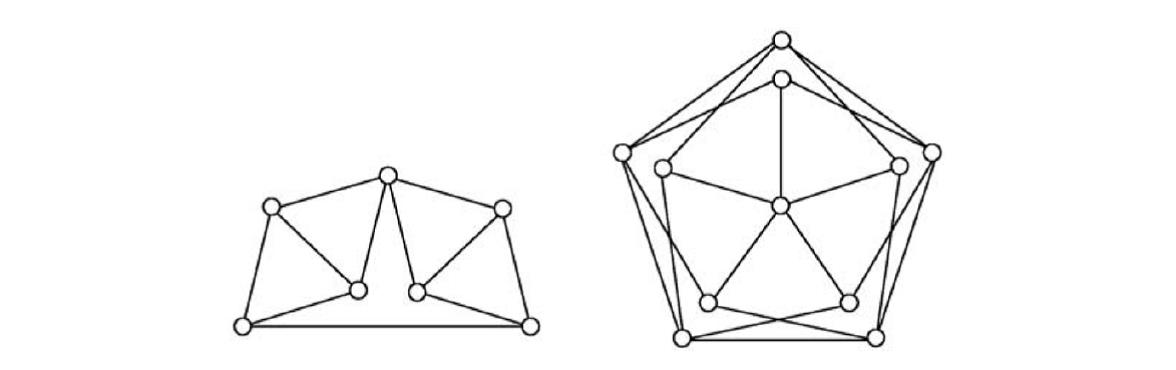
\includegraphics[width=\textwidth]{graph1}
\end{figure}
\end{EXAMPLE}
\end{spacing}
\end{frame}
\begin{frame}[c,allowdisplaybreaks,allowframebreaks]{Maps and Dual Graphs}
\begin{spacing}{1.1}
\vspace*{8pt}
Consider a map of regions, as shown below:
\begin{figure}
  \centering
  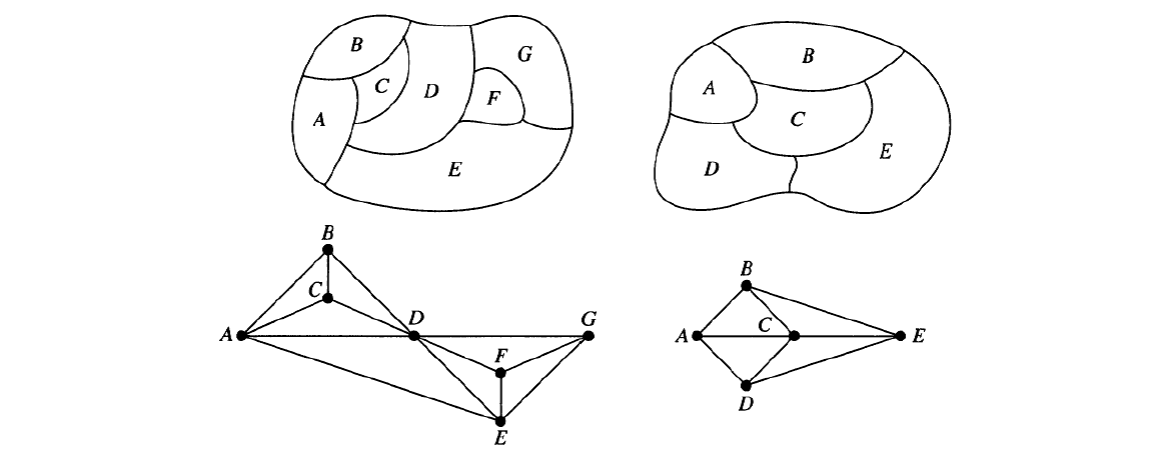
\includegraphics[width=\textwidth]{graph2}
\end{figure}
\begin{center}
\begin{spacing}{0.5}
\begin{tiny}
Image source: Rosen, K.H., \emph{Discrete Mathematics}, 6th Ed., McGraw-Hill International Edition 2007. Used under fair use
exemption.
\end{tiny}
\end{spacing}
\end{center}
\newpage
The \emph{dual graph} is found as follows: choose an arbitrary point in each
region (the dual vertex) and connect the points by drawing a single line
joining them through each distinct border. If a border has two or more
separate components (e.g., the border between Russia and China, which is
interrupted by Mongolia), a single line is sufficient. The system of points
(vertices) and lines (edges) then gives the dual graph, which is always
planar (why?).\\[5pt]
A famous, classic question now is: How many colors are at most necessary
to color a map, or equivalently, it's dual graph?
\end{spacing}
\end{frame}
\begin{frame}[c]{The Four-Color Theorem}
\begin{spacing}{1.2}
The following theorem was first formulated as a conjecture in the 1850s
and was only proven in 1976 with the aid of computers. The (at the time
controversial) proof is the first example of a significant theorem that was
proven in a way that would make it all but impossible for a human being
to verify the result by hand.\\[5pt]
\stepcounter{zhuo}
\alert{3.3.19. Four Color Theorem.} The chromatic number of a planar graph is no greater than four.\\[6pt]
\begin{EXAMPLE}
GSM cell phone networks operate in different frequency
ranges, as adjacent regions need to have different frequencies to prevent
interference. GSM uses only four such ranges, which (by the Four Color
Theorem) is sufficient.
\end{EXAMPLE}
\end{spacing}
\end{frame}
\begin{frame}[c,allowdisplaybreaks,allowframebreaks]{PSLQ, BBP \& More Computer Math}
\begin{spacing}{1.05}
The issues raised by the proof of the Four Color Theorem have become
more apparent in the last few years:
\begin{itemize}
  \item ``Proof algorithms'' have been designed that can automate the proof of theorems in logic. By referring to truth tables and elementary logical rules, in principle it should be possible to automate the process of establishing he truth or falsehood of statements, provided that is possible in the first place.There have been several successes in this approach, which remains an active area of research.
  \item Rather than just proving theorems, computers have also been used to discover theorems. The best-known example is the PSLQ algorithm, that finds relations linking constants to algebraic expressions automatically. In fact, one surprising formula to be discovered in this way is the BBP (Borwein-Bailey-Plouffe) formula in 1996,
      \[\pi=\sum_{k=0}^{\infty}\frac{1}{16^k}\left(\frac{4}{8k+1}-\frac{2}{8k+4}-\frac{1}{8k+5}-\frac{1}{8k+6}\right).\]
\end{itemize}
\newpage
The BBP formula for $\pi$ is remarkable because despite its simple form, it
has escaped detection by humans until it was ``discovered'' by the PSLQ
algorithm. Once discovered, the proof is actually not difficult (see
assignments).\\[5pt]
Furthermore, the formula is also useful, since it can be used to calculate
the $n$th decimal of $\pi$ in hexadecimal expansion without first calculating the
preceding digits. Such formulas are very rare and have recently been
designated ``spigot'' formulas.\\[6pt]
It appears that computers have become an integral part of mathematics,
far beyond performing simple calculations or visualizations.
\end{spacing}
\end{frame}
\subsection{Trees}
\begin{frame}[c] \begin{spacing}{2.5}
\tableofcontents[sectionstyle=hide,subsectionstyle=show/shaded/hide] \end{spacing}
\end{frame}
\begin{frame}[t]{Trees}
\begin{spacing}{1.05}
\begin{DEFINITION}
A \emph{tree} is a connected undirected graph with no simple
circuits. A not necessarily connected graph with no simple circuits is called
a \emph{forest}.\\[6pt]
\end{DEFINITION}
\begin{EXAMPLE}
Of the graphs below, $G_1$ and $G_2$ are trees, while $G_4$ is a forest.
\vspace*{10pt}
\begin{center}
\tikzset{
my state/.style={circle,draw,fill=black,inner sep=0pt,minimum size=1mm}}
  \begin{tikzpicture}[auto,node distance=1.4cm,on grid,every state/.style={fill=black,draw=black},line width=0.25mm]
    \node[my state] (A1) at (0,0){};
    \node[my state] (B1) at (0,1.5){};
    \node[my state] (C1) at (0,3){};
    \node[my state] (D1) at (1.5,0){};
    \node[my state] (E1) at (1.5,1.5){};
    \node[my state] (F1) at (1.5,3){};
    \node[my state] (A2) at (3,0){};
    \node[my state] (B2) at (3,1.5){};
    \node[my state] (C2) at (3,3){};
    \node[my state] (D2) at (4.5,0){};
    \node[my state] (E2) at (4.5,1.5){};
    \node[my state] (F2) at (4.5,3){};
    \node[my state] (A3) at (6,0){};
    \node[my state] (B3) at (6,1.5){};
    \node[my state] (C3) at (6,3){};
    \node[my state] (D3) at (7.5,0){};
    \node[my state] (E3) at (7.5,1.5){};
    \node[my state] (F3) at (7.5,3){};
    \node[my state] (A4) at (9,0){};
    \node[my state] (B4) at (9,1.5){};
    \node[my state] (C4) at (9,3){};
    \node[my state] (D4) at (10.5,0){};
    \node[my state] (E4) at (10.5,1.5){};
    \node[my state] (F4) at (10.5,3){};
    \draw[-] (B1) -- (C1);
    \draw[-] (B1) -- (F1);
    \draw[-] (B1) -- (E1);
    \draw[-] (B1) -- (D1);
    \draw[-] (D1) -- (A1);
    \draw[-] (B2) -- (C2);
    \draw[-] (C2) -- (D2);
    \draw[-] (D2) -- (E2);
    \draw[-] (A2) -- (F2);
    \draw[-] (A2) -- (D2);
    \draw[-] (A3) -- (E3);
    \draw[-] (A3) -- (F3);
    \draw[-] (B3) -- (D3);
    \draw[-] (B3) -- (C3);
    \draw[-] (C3) -- (E3);
    \draw[-] (C3) -- (F3);
    \draw[-] (B4) -- (A4);
    \draw[-] (A4) -- (F4);
    \draw[-] (F4) -- (E4);
    \draw[-] (C4) -- (D4);
    \node[below right=0.6cm] at (A1) {$G_1$};
    \node[below right=0.6cm] at (A2) {$G_2$};
    \node[below right=0.6cm] at (A3) {$G_3$};
    \node[below right=0.6cm] at (A4) {$G_4$};
  \end{tikzpicture}
\end{center}
\end{EXAMPLE}
\end{spacing}
\end{frame}
\begin{frame}[t,allowdisplaybreaks,allowframebreaks]{Trees and Simple Paths}
\begin{spacing}{1.1}
Trees can also be characterized by paths. We first give a theorem on the
existence of simple paths in general undirected graphs.\\[6pt]
\begin{THEOREM}
There is a simple path between every pair of distinct
vertices of a connected undirected graph.\\[6pt]
\end{THEOREM}
\begin{PROOF}
Let $G=(V,E)$ be a connected undirected graph and $u\neq v$ two vertices. Since $G$ is connected, there exists at least one path joining $u$ and $v$. Let $(u,x_1,\,...\,,x_{n-1},v)$ be the tuple of vertices associated to such a path
having least length. We then claim that this path is simple. If it is not
simple, the $x_i=x_j$ for some $i<j$. However, then the tuple of vertices $(x_{i+1},\,...\,,x_j)$ can be eliminated from the path to give a shorter path,
yielding a contradiction.
\end{PROOF}
\newpage
The following theorem gives an equivalent characterization of trees which
is sometimes used as a definition.\\[6pt]
\begin{THEOREM}
An undirected graph is a tree if and only if there is a
unique simple path between any two of its vertices.\\[6pt]
\end{THEOREM}
\begin{PROOF}
\begin{itemize}
  \item[($\Rightarrow$)] Suppose that $T$ is a tree. Then $T$ is a connected graph with no simple circuits. Let $x, y$ be distinct vertices. Then, since $T$ is connected, there exists a simple path joining $x$ and $y$ by Theorem 3.4.3. This path must be unique, for if there were a second such path the two paths could be joined to yield a circuit. This circuit could further be reduced to a simple circuit (see assignments), yielding a contradiction.
\end{itemize}
\newpage
\vspace*{7pt}
\alert{Proof (continued).}
\begin{itemize}
  \item[($\Leftarrow$)] Suppose that $T$ is a graph and that there exists a unique simple path
between any two vertices of $T$. Then $T$ is clearly connected.
Furthermore, $T$ can not have a simple circuit: if there were such a
circuit starting and ending at a vertex $x$ and passing through a vertex
$y$, then there would be two distinct simple paths joining $x$ and $y$. But
this contradicts the assumption that there exists a unique simple path
between $x$ and $y$.
\end{itemize}
\end{PROOF}
\end{spacing}
\end{frame}
\begin{frame}[t,allowdisplaybreaks,allowframebreaks]{Rooted Trees}
\begin{spacing}{1.15}
\vspace*{12pt}
\begin{DEFINITION}
A \emph{rooted tree} is a tree in which one vertex has been
designated as the root and every edge is imbued with a direction in such a
way that the root is the initial vertex of any path joining the root to any
other vertex.\\[7pt]
Definition 3.4.5 suffices to imbue each edge of a tree with a unique direction (why?).
\end{DEFINITION}
\end{spacing}
\newpage
\begin{spacing}{1}
We next introduce some terminology:\\
\begin{DEFINITION}
Let $T$ be a rooted tree with root $r$.
\begin{itemize}
  \item If $v\neq r$ is a vertex in $T$, the \emph{parent} of $v$ is the unique vertex $u$ such that there is a directed edge $(u,v)$ in $T$.
  \item If $u$ is the parent of $v$, the $v$ is a \emph{child} of $u$.
  \item If $v_1,v_2$ have the same parent $u$, they are called \emph{siblings}.
  \item If $v\neq r$, the \emph{ancestors} of $v$ are vertices in the unique directed path joining $r$ to $v$, excluding $v$ and $r$.
  \item The \emph{descendants} of a vertex $u$ are all those vertices which have $u$ as an ancestor.
  \item A vertex with no children is called a \emph{leaf}, otherwise it is called an \emph{internal vertex}.
  \item If $a$ is a vertex in $T$, the rooted subtree with root $a$ is the tree whose vertices comprise $a$ and all its descendants and whose edges comprise all the edges joining $a$ to these descendants.
\end{itemize}
\end{DEFINITION}
\end{spacing}
\end{frame}
\begin{frame}[c]{$m$-ary Trees}
\begin{spacing}{1.1}
\begin{DEFINITION}
A rooted tree is called an \emph{$m$-ary} tree if every internal
vertex has no more than $m$ children. The tree is called a \emph{full $m$-ary tree} if every internal vertex has exactly $m$ children. A (full) $m$-ary tree with $m = 2$ is called a \emph{(full) binary tree}.\\[6pt]
\end{DEFINITION}
\begin{DEFINITION}
An \emph{ordered rooted tree} is a tree where the children of each vertex are ordered.\\[6pt]
\end{DEFINITION}
When drawing a rooted tree in the conventional way, we consider the
children to be ordered from left to right. Unless stated otherwise, all
depicted trees are considered to be ordered in this way.\\[6pt]
For (ordered) binary trees we define the \emph{left child} and the \emph{right child} of a
root in the obvious way. If $u$ is an internal vertex, the (rooted) subtree
with the left/right child of $u$ as its root is called the \emph{left/right subtree of $u$}.
\end{spacing}
\end{frame}
\begin{frame}[t,allowdisplaybreaks,allowframebreaks]{Application to Saturated Hydrocarbons}
\begin{spacing}{1}
\vspace*{-7pt}
A \emph{saturated hydrocarbon}, or \emph{alkane}, has the chemical formula $\text{C}_n\text{H}_{2n+2}$. Examples include
\begin{center}
\tikzset{
my state/.style={circle,draw=white,fill=white,inner sep=0pt,minimum size=4mm}}
\begin{tikzpicture}[node distance=1cm,on grid,
every state/.style={draw=black,fill=white,text=black,very thick},line width=0.3mm]
\node[my state] (A) at (0,0) {C};
\node[my state] (B) at (-0.8,0) {H};
\node[my state] (C) at (0.8,0) {H};
\node[my state] (D) at (0,0.8) {H};
\node[my state] (E) at (0,-0.8) {H};
\node[above=0.2cm] at (D) {Methane (CH\textsubscript{4})};
\draw[-] (A) to (B);
\draw[-] (A) to (D);
\draw[-] (A) to (C);
\draw[-] (A) to (E);
\node[my state] (F) at (3.2,0) {C};
\node[my state] (G) at (4,0) {C};
\node[my state] (H) at (3.2,0.8) {H};
\node[my state] (I) at (4,0.8) {H};
\node[my state] (J) at (3.2,-0.8) {H};
\node[my state] (K) at (4,-0.8) {H};
\node[my state] (L) at (2.4,0) {H};
\node[my state] (M) at (4.8,0) {H};
\draw[-] (F) to (H);
\draw[-] (F) to (J);
\draw[-] (G) to (I);
\draw[-] (G) to (K);
\draw[-] (F) to (L);
\draw[-] (G) to (M);
\draw[-] (F) to (G);
\node[above=0.2cm] at (3.6,0.8) {Ethane (C\textsubscript{2}H\textsubscript{6})};
\node[my state] (N) at (6.6,0) {C};
\node[my state] (O) at (7.4,0) {C};
\node[my state] (P) at (8.2,0) {C};
\node[my state] (Q) at (6.6,0.8) {H};
\node[my state] (R) at (6.6,-0.8) {H};
\node[my state] (S) at (7.4,0.8) {H};
\node[my state] (T) at (7.4,-0.8) {H};
\node[my state] (U) at (8.2,0.8) {H};
\node[my state] (V) at (8.2,-0.8) {H};
\node[my state] (W) at (5.8,0) {H};
\node[my state] (X) at (9,0) {H};
\draw[-] (N) to (Q);
\draw[-] (N) to (R);
\draw[-] (N) to (W);
\draw[-] (N) to (O);
\draw[-] (O) to (S);
\draw[-] (O) to (T);
\draw[-] (O) to (P);
\draw[-] (P) to (U);
\draw[-] (P) to (V);
\draw[-] (P) to (X);
\node[above=0.2cm] at (S) {Propane (C\textsubscript{3}H\textsubscript{8})};
\end{tikzpicture}
\end{center}
\begin{center}
\tikzset{
my state/.style={circle,draw=white,fill=white,inner sep=0pt,minimum size=4mm}}
\begin{tikzpicture}[line width=0.3mm]
\node[my state] (A) at (0,0) {H};
\node[my state] (B) at (0.8,0) {C};
\node[my state] (C) at (0.8,0.8) {H};
\node[my state] (D) at (0.8,-0.8) {H};
\node[my state] (E) at (1.6,0) {C};
\node[my state] (F) at (1.6,0.8) {H};
\node[my state] (G) at (1.6,-0.8) {H};
\node[my state] (H) at (2.4,0) {C};
\node[my state] (I) at (2.4,0.8) {H};
\node[my state] (J) at (2.4,-0.8) {H};
\node[my state] (K) at (3.2,0) {C};
\node[my state] (L) at (3.2,0.8) {H};
\node[my state] (M) at (3.2,-0.8) {H};
\node[my state] (N) at (4,0) {H};
\draw[-] (B) to (A);
\draw[-] (B) to (C);
\draw[-] (B) to (D);
\draw[-] (B) to (E);
\draw[-] (E) to (F);
\draw[-] (E) to (G);
\draw[-] (E) to (H);
\draw[-] (H) to (I);
\draw[-] (H) to (J);
\draw[-] (H) to (K);
\draw[-] (K) to (L);
\draw[-] (K) to (M);
\draw[-] (K) to (N);
\node[above=0.2cm] at (2,0.8) {$n$-Butane (C\textsubscript{4}H\textsubscript{10})};
\tikzset{
my state/.style={circle,draw=white,fill=white,inner sep=0pt,minimum size=3mm}}
\node[my state] (O) at (5.6,0) {H};
\node[my state] (P) at (6.4,0) {C};
\node[my state] (Q) at (6.4,0.8) {H};
\node[my state] (R) at (6.4,-0.8) {H};
\node[my state] (S) at (7.4,0) {C};
\node[my state] (T) at (7.4,0.8) {H};
\node[my state] (U) at (7.4,-0.8) {C};
\node[my state] (V) at (6.9,-0.8) {H};
\node[my state] (W) at (7.9,-0.8) {H};
\node[my state] (X) at (7.4,-1.3) {H};
\node[my state] (Y) at (8.4,0) {C};
\node[my state] (Z) at (8.4,0.8) {H};
\node[my state] (AA) at (8.4,-0.8) {H};
\node[my state] (AB) at (9.2,0) {H};
\draw[-] (O) to (P);
\draw[-] (P) to (Q);
\draw[-] (P) to (R);
\draw[-] (P) to (S);
\draw[-] (S) to (T);
\draw[-] (S) to (U);
\draw[-] (U) to (V);
\draw[-] (U) to (W);
\draw[-] (U) to (X);
\draw[-] (S) to (Y);
\draw[-] (Y) to (Z);
\draw[-] (Y) to (AA);
\draw[-] (Y) to (AB);
\node[above=0.2cm] at (T) {iso-Butane (Methylpropane; C\textsubscript{4}H\textsubscript{10})};
\end{tikzpicture}
\end{center}
\newpage
We can define saturated hydrocarbons inductively as follows:\\
\begin{DEFINITION}
\begin{itemize}
  \item[(i)] The rooted tree consisting of one root and four children is an alkane.
  \item[(ii)] If $T$ is a rooted tree, then the tree obtained by adding three children to a leaf is an alkane.
\end{itemize}
In this definition, the internal vertices will represent carbon atoms, while
the leaves represent hydrogen atoms.\\[5pt]
Definition 3.4.9 will yield alkanes that are different regarded as rooted
trees, but whose underlying undirected graphs are isomorphic. These are
considered to represent the same molecule.\\[5pt]
Alkanes with the same number of internal vertices and the same number
of leaves that are not isomorphic are called \emph{stereoisomers}. Finding the
number of stereoisomers of a given compound is a non-trivial problem
involving graphs and counting. More information on this problem can be
found at \url{http://www.cs.uwaterloo.ca/journals/JIS/cayley.html}
\end{DEFINITION}
\end{spacing}
\end{frame}
\begin{frame}[t,allowdisplaybreaks,allowframebreaks]{Counting the Vertices and Edges of Trees}
\begin{spacing}{1.05}
\vspace*{9pt}
\begin{THEOREM}
A tree with $n$ vertices has $n-1$ edges.\\[7pt]
\end{THEOREM}
\begin{PROOF}
The proof follows easily by induction: for $n = 1$ the tree consists only of a
single vertex and no edges, so the statement is true.\\[7pt]
Suppose the statement is true for any tree with $n$ vertices and let $T$ be a
tree with $n + 1$ vertices. Then $T$ has a leaf, which can be removed along
with the vertex joining it to its parent. The resulting tree has $n$ vertices, and, by the induction hypothesis, $n - 1$ edges. Restoring the eliminated leaf and its edge, we see that $T$ has $n$ edges.
\end{PROOF}
\newpage
\begin{THEOREM}
A full $m$-ary tree with $i$ internal vertices contains $n=mi+1$ vertices.\\[7pt]
\begin{PROOF}
There are two types of vertices in a full $m$-ary tree: the root and vertices
that are children of other vertices. Since there are $i$ internal vertices, there
must be $m\cdot i$ children. Adding the root, we obtain $n=mi+1$.
\end{PROOF}
\begin{THEOREM}
A full $m$-ary tree with
\begin{itemize}
  \item[(i)] $n$ vertices has $i=(n-1)/m$ internal vertices and $I=[(m-1)n+1]/m$ leaves,
  \item[(ii)] $i$ internal vertices has $n=mi+1$ vertices and $I=(m-1)i+1$ leaves,
  \item[(iii)] $I$ leaves has $n=(ml-1)/(m-1)$ vertices and $i=(I-1)/(m-1)$ internal vertices.
\end{itemize}
\begin{PROOF}
The theorem follows from the two equations $n=mi+1$ and $n=i+l$.
\end{PROOF}
\end{THEOREM}
\end{THEOREM}
\newpage
\vspace*{11pt}
\begin{EXAMPLE}
Suppose that someone starts a chain letter. Each person
who receives the letter is asked to send it on to four other people. Some
people do this, but others do not send any letters. How many people have
seen the letter, including the first person, if no one receives more than one
letter and if the chain letter ends after there have been 100 people who
read it but did not send it out? How many people sent out the letter?
\end{EXAMPLE}
\end{spacing}
\end{frame}
\begin{frame}[t,allowdisplaybreaks,allowframebreaks]{Balanced $m$-ary Trees}
\begin{spacing}{1.2}
\begin{DEFINITION}
Let $T$ be a rooted tree with root $r$.
\begin{itemize}
  \item The \emph{level} of a vertex $v\neq r$ is the length of the path joining $r$ to $v$. The level of $r$ is defined to be zero.
  \item The \emph{height} of $T$ is the maximum of all the levels of the vertices of $T$.
  \item A rooted $m$-ary tree of height $h$ is said to be \emph{balanced} if all leaves have levels $h$ or $h-1$.
\end{itemize}
\end{DEFINITION}
\vspace*{5pt}
\begin{THEOREM}
An $m$-ary tree of height $h$ has at most $m^h$ leaves.\\
\end{THEOREM}
\vspace*{5pt}
\begin{PROOF}
We prove the statement by strong induction in $h$. The statement is true
for $h = 0$, because the tree then consists of a single vertex, the root. This is a leaf, so the number of leaves is $m^0=1$.
\newpage
\vspace*{5pt}
\alert{Proof (continued).}\\
Assume $T$ is a tree of height $h$. Removing the root and all edges
originating at the root, one obtains a forest of at most $m$ tress of height at
most $h-1$. Each tree has at most $m^{h-1}$ leaves by the induction
hypothesis. Hence, the total number of leaves is at most $m\cdot m^{h-1}=m^h$.
\end{PROOF}
\vspace*{5pt}
\begin{COROLLARY}
\begin{itemize}
  \item[(i)] If an $m$-ary tree of height $h$ has $l$ leaves, then $h\geq\lceil\log_ml\rceil$.
  \item[(ii)] If the $m$-ary tree is full and balanced, then $h=\lceil\log_ml\rceil$.
\end{itemize}
\end{COROLLARY}
\begin{PROOF}
Statement (i) follows directly from $l\leq m^h\Leftrightarrow h\geq\log_ml$. Statement (ii) will be proven in the assignments.
\end{PROOF}
\end{spacing}
\end{frame}
\begin{frame}[c]{Binary Search Trees}
\begin{spacing}{1.15}
Suppose we have a totally ordered set of objects that we want to enter
into a database for easy lookup. One technique involves the use of binary
trees as follows:
\begin{itemize}
  \item[1.] The first object becomes the root of the search tree.
  \item[2.] The second object becomes a left child if it precedes the root, or a right child if it succeeds it.
  \item[3.] The third and further objects are sorted along the tree, moving left if they precede a vertex or right if they succeed it.
\end{itemize}
\begin{EXAMPLE}
We enter the words mathematics, physics, geography,
zoology, meteorology, geology, psychology, and chemistry (in this order)
into a search tree, using the standard lexicographic ordering of words.
\end{EXAMPLE}
\end{spacing}
\end{frame}
\begin{frame}[t,allowdisplaybreaks,allowframebreaks]{Locating and Adding Items to a Binary Search Tree}
\begin{spacing}{1.05}
\stepcounter{zhuo}
\alert{3.4.18. Algorithm.} \emph{(Locating or adding items to a binary search tree)}
\IncMargin{1em}
\begin{algorithm}[H]
\SetKwInput{Kw}{Input}\SetKwInput{Kt}{Output}
\SetKwIF{If}{ElseIf}{Else}{if}{then}{else if}{else}{end~if}
\SetKwFor{While}{while}{do}{end~while}
\Kw{$T$ a binary search tree and $x$ an item to be found or added}
\Kt{$v$ the position of $x$ in the binary tree}
$v\leftarrow$ root of $T$\;
\lIf{$v=NULL$}{$v\leftarrow x$;}~\Return{$v$}\;
\While{$v.label\neq x.label$}{
\eIf{$x.label<v.label$}{
\lIf{$v.left=NULL$}{$v.left\leftarrow x$}\;
$v\leftarrow v.left$\;}{
\lIf{$v.right=NULL$}{$v.right\leftarrow x$}\;
$v\leftarrow v.right$\;}}
\Return {$v$}
\end{algorithm}\DecMargin{1em}
\end{spacing}
\newpage
\begin{spacing}{0.95}
We now analyze the computational complexity of Algorithm 3.4.18. First,
given a binary tree $T$ with $n$ labeled vertices, we add unlabeled vertices to
it so that every labeled vertex has two children. This gives a full binary
tree, which we denote by $U$. The labeled vertices are the interior vertices
of $U$. The advantage of this procedure is that when locating or adding an
item, we never increase the number of vertices in $U$.\\[6pt]
The most comparisons needed to add an item is the length of the longest
path in $U$ from its root to a leaf, i.e., the height $h$ of $U$. The vertices of $T$
are the interior vertices of $U$, so $U$ has $n$ interior vertices. By Theorem
3.4.12, $U$ then has $n+1$ leaves. Corollary 3.4.16 gives
\[h\geq\lceil\log_2(n+1)\rceil.\]
If $T$ is balanced we actually have equality, so the algorithm requires at most $\lceil\log(n+1)\rceil=O(\log n)$ comparisons. As items are added to a search tree, it may become unbalanced. There are algorithms (discussed in
courses on data structures) that can ``rebalance'' a tree in this case.
\end{spacing}
\end{frame}
\begin{frame}[c]{Decision Trees}
\begin{spacing}{1.2}
A rooted tree in which each internal vertex corresponds to a decision, with
a subtree at these vertices for each possible outcome of the decision, is
called a \emph{decision tree}. The possible solutions of the problem correspond to
the paths to the leaves of this rooted tree. This is illustrated through the
following example:\\[6pt]
\begin{EXAMPLE}
Suppose that among eight nominally identical coins one
is counterfeit and lighter than the others. This coin may be found by
weighing any number of the eight coins on a balance scale. We wish do
determine the minimum number of weighings needed to find the
counterfeit coin.
\end{EXAMPLE}
\end{spacing}
\end{frame}
\begin{frame}[t,allowdisplaybreaks,allowframebreaks]{Finding a Counterfeit Coin}
\begin{spacing}{1.1}
\vspace*{10pt}
Every weighing corresponds to an internal vertex in a decision tree and
every result is a child of this weighing and also corresponds to the next
weighing. Each weighing has three possible outcomes:
\begin{itemize}
  \item ``left side is lighter''
  \item ``right side is lighter''
  \item ``no side is lighter''
\end{itemize}
so the decision tree is a 3-ary tree. The final result after the weighings (``coin no. $n$ is counterfeit'') corresponds to a leaf in the tree. There are 8 possible leaves, so, by Corollary 3.4.16 the height of the tree is at least $\lceil\log_38\rceil=2$. Hence, at least 2 weighings are necessary.
\newpage
\vspace*{10pt}
A naive approach easily shows that the coin can be found in three
weighings. However, it is also possible to do so in just two weighings, as
illustrated below:\\
\includegraphics[width=\textwidth]{weighing}\\
\begin{center}
\begin{spacing}{0.5}
\begin{tiny}
Image source: Rosen, K.H., \emph{Discrete Mathematics}, 6\textsuperscript{th} Ed., McGraw-Hill International Edition 2007. Used under fair use
exemption.
\end{tiny}
\end{spacing}
\end{center}
\end{spacing}
\end{frame}
\begin{frame}[c]{Complexity of Binary Sorting Algorithms}
\begin{spacing}{1.1}
Consider a sorting algorithm based on comparing two configurations of a
given list (usually by comparing two possible positions of a single list
item). Such an algorithm is called a \emph{binary sorting algorithm}, because each
comparison will designate one of two possible list configurations as being
``more sorted''. All of the sorting algorithms we have studied are of this
type.\\[6pt]
We can model any binary sort algorithm using a binary decision tree. For a
list of $n$ distinct elements there are $n!$ different arrangements, one of which
will correspond to the sorted list. Hence, the decision tree has $n!$ leaves and, by Corollary 3.4.16 the height of the tree is at least $\lceil\log_2(n!)\rceil$ and at least that many comparisons are needed.\\[6pt]
We now conduct a brief excursion into calculus to obtain an estimate for $\log_2(n!)$.
\end{spacing}
\end{frame}
\begin{frame}[t,allowdisplaybreaks,allowframebreaks]{Elementary Estimate on the Factorial}
\begin{spacing}{0.4}
We may obtain an elementary estimate as follows: Let
\[S_n=\ln(n!)=\sum_{k=1}^{n}\ln k.\]
Then it is easy to see that
\setcounter{equation}{0}
\begin{equation}\label{3.4.1}
\int_{1}^{n+1}\ln x\,dx>S_n>\int_{2}^{n+1}\ln(x-1)\,dx=\int_{1}^{n}\ln x\,dx.
\end{equation}
\begin{center}
\begin{tikzpicture}[domain=1:7]
\draw[-latex,scale=1] (0,0) -- (8,0) node[right] {$x$};
\draw[-latex,scale=1.1] (0,0) -- (0,2.4) node[above] {$y$};
\draw[color=green,line width=0.25mm] plot (\x,{ln(\x)}) node[above] {};
\foreach \x in {2,...,6}
\draw[fill=blue!10,draw=none](\x,0) rectangle +(1,{ln(\x)});
\draw[color=purple,line width=0.25mm,domain=2:7] plot (\x,{ln(\x-1)}) node[above] {};
\foreach \z in {2,...,6}
\draw[color=blue,line width=0.25mm,domain=\z:{\z+1}] plot (\x,{ln(\z)});
\node at (4,{ln(7)}) {\scriptsize$y=\ln(x)$};
\node at (6,{ln(3)}) {\scriptsize$y=\ln(x-1)$};
\foreach \z in {1,...,7}
\filldraw[black] (\z,0) circle (0.3mm);
\foreach \z in {2,...,7}
\filldraw[black] (0,{ln(\z)}) circle (0.3mm);
\foreach \z in {1,...,7}
\node at (\z,-0.2) {\tiny$\z$};
\foreach \z in {2,...,7}
\node at (-0.3,{ln(\z)}) {\tiny$\ln(\z)$};
\end{tikzpicture}
\end{center}
\end{spacing}
\newpage
\begin{spacing}{1.1}
\vspace*{10pt}
Since $\int\ln(x)\,dx=x\ln(x)-x$, we immediately obtain
\[n\ln(n)-n-e+1<\ln(n!)<(n+1)\ln(n+1)-n-e.\]
This implies that $\log n!=\Theta(n\log n)$. It follows that the worst-case time complexity of any binary sort is $\Omega(n\log n)$. Thus, it is impossible to find a binary search algorithm that has a lower time complexity than $O(n\log n)$. The merge sort (Algorithm 2.1.27) may be considered optimal in this sense.
\end{spacing}
\end{frame}
\begin{frame}[t,allowdisplaybreaks,allowframebreaks]{Prefix Codes}
\begin{spacing}{1.1}
Another type of decision tree occurs when encoding letters as binary digits.
Suppose that we want to encode the letters e, a and t. If we simply set
\[e\mapsto 0,\qquad\qquad\quad a\mapsto 1,\qquad\qquad\quad t\mapsto 01,\]
then the string 0101 could represent either ``eaea'' or ``tt'' or ``eat''. We
would therefore like to find a method that encodes letters as strings
without ambiguity. More precisely, we want to ensure that the bit string
encoding of a letter never occurs as the first part of the encoding for any
other letter. Encodings with this property are called \emph{prefix codes}.\\[6pt]
We can construct prefix codes from binary trees as follows: suppose we
want to encode the letters e, a, t, n and s. Then we assign each letter the
code found by concatenating the labels of the edges of the path joining
the root to the letter in the following tree.
\newpage
\begin{center}
\tikzset{
my state/.style={circle,draw,fill=black,inner sep=0pt,minimum size=1.5mm},
my state2/.style={circle,fill=white,inner sep=0pt,minimum size=4mm}}
\begin{tikzpicture}[auto,node distance=1.4cm,on grid,every state/.style={fill=black,draw=black},line width=0.25mm]
\node[my state] (n) at (0,0) {};
\node[my state] (s) at (2,0) {};
\node[my state] (ns) at (1,1) {};
\node[my state] (t) at (-1,1) {};
\node[my state] (tns) at (0,2) {};
\node[my state] (a) at (-2,2) {};
\node[my state] (atns) at (-1,3) {};
\node[my state] (e) at (-3,3) {};
\node[my state] (eatns) at (-2,4) {};
\node[my state2] (1) at (-2.5,3.5) {0};
\node[my state2] (2) at (-1.5,3.5) {1};
\node[my state2] (3) at (-1.5,2.5) {0};
\node[my state2] (4) at (-0.5,2.5) {1};
\node[my state2] (5) at (-0.5,1.5) {0};
\node[my state2] (6) at (0.5,1.5) {1};
\node[my state2] (7) at (0.5,0.5) {0};
\node[my state2] (8) at (1.5,0.5) {1};
\node[below=0.2cm] at (e) {$e$};
\node[below=0.2cm] at (a) {$a$};
\node[below=0.2cm] at (t) {$t$};
\node[below=0.2cm] at (n) {$n$};
\node[below=0.2cm] at (s) {$s$};
\draw[-] (e) to (1) (1) to (eatns) (eatns) to (2) (2) to (atns) (a) to (3) (3) to (atns) (atns) to (4) (4) to (tns) (t) to (5) (5) to (tns) (tns) to (6) (6) to (ns) (n) to (7) (7) to (ns) (ns) to (8) (8) to (s);
\end{tikzpicture}
\end{center}
Hence we have
\[e\mapsto 0,\qquad a\mapsto 10,\qquad t\mapsto 110,\qquad n\mapsto 1110,\qquad s\mapsto 1111.\]
\end{spacing}
\end{frame}
\begin{frame}[t,allowdisplaybreaks,allowframebreaks]{Huffman Coding}
\begin{spacing}{1.05}
Clearly, a prefix code uses longer bit strings to ensure the non-ambiguity of
the encoding. Given a text that is to be encoded, we would like to
minimize the total number of bits necessary for the encoding. Thus, we
would like to encode common letters using short bit strings and rarely
occurring letters using longer bit strings. One algorithm that implements
this goal is called \emph{Huffman coding}.\\[6pt]
Huffman encoding works as follows: an initial forest of rooted trees
consisting of a single vertex labeled with the letters and their frequencies is
given. In each step, the two trees with the smallest labels are joined to a
new root, which is labeled with the sum of the labels of the roots of the
two trees. This is repeated until a single tree is obtained. The left children
are labeled with zeroes while the right children are labeled with ones.\\[6pt]
Huffman coding is a greedy algorithm and it is optimal in the sense that
no binary prefix code can encode symbols (letters) using fewer bits. This
will be shown in the assignments.
\end{spacing}
\newpage
\begin{spacing}{0.75}
\begin{EXAMPLE}
Suppose it is known that the following letters appear
with the given frequencies:
\[A:0.08,\qquad B:0.10,\qquad C:0.12,\qquad D:0.15,\qquad E:0.20,\qquad F:0.35.\]
We then have the following iterative trees:
\begin{center}
\tikzset{
my state/.style={circle,draw,fill=black,inner sep=0pt,minimum size=1.5mm}}
\vspace*{-6pt}
\begin{tikzpicture}[auto,node distance=1.4cm,on grid,every state/.style={fill=black,draw=black},line width=0.25mm]
\node[my state] (a) at (0,0) {};
\node[my state] (b) at (2,0) {};
\node[my state] (c) at (4,0) {};
\node[my state] (d) at (6,0) {};
\node[my state] (e) at (8,0) {};
\node[my state] (f) at (10,0) {};
\node[below=0.2cm] at (a) {A\:0.08};
\node[below=0.2cm] at (b) {B\:0.10};
\node[below=0.2cm] at (c) {C\:0.12};
\node[below=0.2cm] at (d) {D\:0.15};
\node[below=0.2cm] at (e) {E\:0.20};
\node[below=0.2cm] at (f) {F\:0.35};
\end{tikzpicture}
\tikzset{
my state2/.style={circle,fill=white,inner sep=0pt,minimum size=3mm}}
\vspace*{-6pt}
\begin{tikzpicture}[auto,node distance=1.4cm,on grid,every state/.style={fill=black,draw=black},line width=0.25mm]
\node[my state] (c) at (0.1,0) {};
\node[my state] (d) at (2.2,0) {};
\node[my state] (a) at (4.1,0) {};
\node[my state] (b) at (6,0) {};
\node[my state] (e) at (7.9,0) {};
\node[my state] (f) at (10,0) {};
\node[my state] (ab) at (5.05,0.8) {};
\node[my state2] (1) at (4.575,0.4) {0};
\node[my state2] (2) at (5.525,0.4) {1};
\node[below=0.2cm] at (a) {A};
\node[below=0.2cm] at (b) {B};
\node[below=0.2cm] at (c) {C\:0.12};
\node[below=0.2cm] at (d) {D\:0.15};
\node[below=0.2cm] at (e) {E\:0.20};
\node[below=0.2cm] at (f) {F\:0.35};
\node[above=0.2cm] at (ab) {0.18};
\draw[-] (a) to (1) (1) to (ab) (ab) to (2) (2) to (b);
\end{tikzpicture}
\begin{tikzpicture}[auto,node distance=1.4cm,on grid,every state/.style={fill=black,draw=black},line width=0.25mm]
\node[my state] (a) at (-0.1,0) {};
\node[my state] (b) at (2,0) {};
\node[my state] (e) at (3.8,0) {};
\node[my state] (c) at (5.9,0) {};
\node[my state] (d) at (7.8,0) {};
\node[my state] (f) at (9.9,0) {};
\node[my state] (ab) at (0.95,0.8) {};
\node[my state] (cd) at (6.85,0.8) {};
\node[my state2] (1) at (0.425,0.4) {0};
\node[my state2] (2) at (1.475,0.4) {1};
\node[my state2] (3) at (6.375,0.4) {0};
\node[my state2] (4) at (7.325,0.4) {1};
\node[below=0.2cm] at (a) {A};
\node[below=0.2cm] at (b) {B};
\node[below=0.2cm] at (c) {C};
\node[below=0.2cm] at (d) {D};
\node[below=0.2cm] at (e) {E\:0.20};
\node[below=0.2cm] at (f) {F\:0.35};
\node[above=0.2cm] at (ab) {0.18};
\node[above=0.2cm] at (cd) {0.27};
\draw[-] (c) to (3) (3) to (cd) (cd) to (4) (4) to (d);
\draw[-] (a) to (1) (1) to (ab) (ab) to (2) (2) to (b);
\end{tikzpicture}
\end{center}
\end{EXAMPLE}
\end{spacing}
\newpage
\begin{spacing}{1.05}
\begin{center}
\tikzset{
my state/.style={circle,draw,fill=black,inner sep=0pt,minimum size=1.5mm},
my state2/.style={circle,fill=white,inner sep=0pt,minimum size=3mm}}
\begin{tikzpicture}[auto,node distance=1.4cm,on grid,every state/.style={fill=black,draw=black},line width=0.25mm]
\node[my state] (c) at (0,0) {};
\node[my state] (d) at (1.5,0) {};
\node[my state] (f) at (3,0) {};
\node[my state] (a) at (4.5,0) {};
\node[my state] (b) at (6,0) {};
\node[my state] (e) at (6.75,0.75) {};
\node[my state] (cd) at (0.75,0.75) {};
\node[my state] (ab) at (5.25,0.75) {};
\node[my state] (abe) at (6,1.5) {};
\node[my state2] (1) at (0.375,0.375) {0};
\node[my state2] (2) at (1.125,0.375) {1};
\node[my state2] (3) at (4.875,0.375) {0};
\node[my state2] (4) at (5.625,0.375) {1};
\node[my state2] (5) at (5.625,1.125) {0};
\node[my state2] (6) at (6.375,1.125) {1};
\node[below=0.2cm] at (a) {A};
\node[below=0.2cm] at (b) {B};
\node[below=0.2cm] at (c) {C};
\node[below=0.2cm] at (d) {D};
\node[below=0.2cm] at (e) {E};
\node[below=0.2cm] at (f) {F\:0.35};
\node[above=0.2cm] at (cd) {0.27};
\node[above=0.2cm] at (abe) {0.38};
\draw[-] (c) to (1) (1) to (cd) (cd) to (2) (2) to (d) (a) to (3) (3) to (ab) (ab) to (4) (4) to (b) (ab) to (5) (5) to (abe) (abe) to (6) (6) to (e);
\end{tikzpicture}\\
\vspace*{12pt}
\begin{tikzpicture}[auto,node distance=1.4cm,on grid,every state/.style={fill=black,draw=black},line width=0.25mm]
\node[my state] (a) at (4.5,0) {};
\node[my state] (b) at (6,0) {};
\node[my state] (e) at (6.75,0.75) {};
\node[my state] (ab) at (5.25,0.75) {};
\node[my state] (abe) at (6,1.5) {};
\node[my state2] (3) at (4.875,0.375) {0};
\node[my state2] (4) at (5.625,0.375) {1};
\node[my state2] (5) at (5.625,1.125) {0};
\node[my state2] (6) at (6.375,1.125) {1};
\node[below=0.2cm] at (a) {A};
\node[below=0.2cm] at (b) {B};
\node[below=0.2cm] at (e) {E};
\node[above=0.2cm] at (abe) {0.38};
\draw[-] (a) to (3) (3) to (ab) (ab) to (4) (4) to (b) (ab) to (5) (5) to (abe) (abe) to (6) (6) to (e);
\node[my state] (c) at (9,0) {};
\node[my state] (d) at (10.5,0) {};
\node[my state] (f) at (11.25,0.75) {};
\node[my state] (cd) at (9.75,0.75) {};
\node[my state] (cdf) at (10.5,1.5) {};
\node[my state2] (7) at (9.375,0.375) {0};
\node[my state2] (8) at (10.125,0.375) {1};
\node[my state2] (9) at (10.125,1.125) {0};
\node[my state2] (10) at (10.875,1.125) {1};
\node[below=0.2cm] at (c) {C};
\node[below=0.2cm] at (d) {D};
\node[below=0.2cm] at (f) {F};
\node[above=0.2cm] at (cdf) {0.62};
\draw[-] (c) to (7) (7) to (cd) (cd) to (8) (8) to (d) (cd) to (9) (9) to (cdf) (cdf) to (10) (10) to (f);
\end{tikzpicture}
\end{center}
\newpage
\begin{center}
\tikzset{
my state/.style={circle,draw,fill=black,inner sep=0pt,minimum size=1.5mm},
my state2/.style={circle,fill=white,inner sep=0pt,minimum size=3mm}}
\begin{tikzpicture}[auto,node distance=1.4cm,on grid,every state/.style={fill=black,draw=black},line width=0.25mm]
\node[my state] (a) at (4.5,0) {};
\node[my state] (b) at (6,0) {};
\node[my state] (e) at (6.75,0.75) {};
\node[my state] (ab) at (5.25,0.75) {};
\node[my state] (abe) at (6,1.5) {};
\node[my state2] (3) at (4.875,0.375) {0};
\node[my state2] (4) at (5.625,0.375) {1};
\node[my state2] (5) at (5.625,1.125) {0};
\node[my state2] (6) at (6.375,1.125) {1};
\node[below=0.2cm] at (a) {A};
\node[below=0.2cm] at (b) {B};
\node[below=0.2cm] at (e) {E};
\draw[-] (a) to (3) (3) to (ab) (ab) to (4) (4) to (b) (ab) to (5) (5) to (abe) (abe) to (6) (6) to (e);
\node[my state] (c) at (6.75,0) {};
\node[my state] (d) at (8.25,0) {};
\node[my state] (f) at (9,0.75) {};
\node[my state] (cd) at (7.5,0.75) {};
\node[my state] (cdf) at (8.25,1.5) {};
\node[my state2] (7) at (7.125,0.375) {0};
\node[my state2] (8) at (7.875,0.375) {1};
\node[my state2] (9) at (7.875,1.125) {0};
\node[my state2] (10) at (8.625,1.125) {1};
\node[below=0.2cm] at (c) {C};
\node[below=0.2cm] at (d) {D};
\node[below=0.2cm] at (f) {F};
\node[below=0.2cm] at (a) {A};
\node[below=0.2cm] at (b) {B};
\node[below=0.2cm] at (e) {E};
\draw[-] (c) to (7) (7) to (cd) (cd) to (8) (8) to (d) (cd) to (9) (9) to (cdf) (cdf) to (10) (10) to (f);
\node[my state] (abcdef) at (7.125,2.625) {};
\node[my state2] (12) at (6.5625,2.0625) {0};
\node[my state2] (13) at (7.6875,2.0625) {1};
\draw[-] (abe) to (12) (12) to (abcdef) (abcdef) to (13) (13) to (cdf);
\end{tikzpicture}
\end{center}
Huffman coding thus gives
\[A\mapsto 000,\qquad B\mapsto 001,\qquad C\mapsto 100,\qquad D\mapsto 101,\qquad E\mapsto 01,\qquad F\mapsto 11.\]
Huffman coding leads to the shortest number of bits used for encoding the
text with the given symbol frequencies (see assignments). The scheme has
been refined in various ways, for example to account for initially unknown
symbol frequencies that are continually updated as more text is encoded.
\end{spacing}
\end{frame}
\begin{frame}[c]{Universal Address System}
\begin{spacing}{1.1}
Many types of trees (such as binary search trees) store information, so
handling this data becomes important. The basis is a systematic way of
labeling the vertices of trees.\\[7pt]
\stepcounter{zhuo}
\alert{3.4.21. Universal Address System.}
\begin{itemize}
  \item[(i)] Label the root with the integer 0. Then label its $k$ children (at level 1) from left to right with $1,\,2,\,3,\,...\,,k$.
  \item[(ii)] For each vertex $v$ at level $n$ with label $A$, label its $k_v$ children, as they are drawn from left to right, with $A.1,\,A.2,\,...\,,A.k_v$.
\end{itemize}
\vspace*{5pt}
The Universal Address System gives a total ordering of the vertices in a
tree through the lexicographic ordering of its labels.
\end{spacing}
\end{frame}
\begin{frame}[c]{Tree Traversal (Preorder)}
\begin{spacing}{1.1}
We now consider the problem of \emph{traversing} an entire tree, i.e., listing
(\emph{visiting}) each vertex of a tree. There are three basic algorithms that
achieve this: \emph{preorder traversal, inorder traversal} and \emph{postorder traversal}.
We will give recursive definitions for each of them.\\[6pt]
\begin{DEFINITION}
Let $T$ be an ordered rooted tree with root $r$.
\begin{itemize}
  \item[(i)] If $T$ consists only of $r$, then $r$ is the preorder traversal of $T$.
  \item[(ii)] If $T_1,\,T_2,\,...\,,T_n$ are the subtrees at $r$ from left to right in $T$, the preorder traversal begins by visiting $r$. Then, $T_1,\,T_2,\,...\,,T_n$ are sequentially traversed in preorder.
\end{itemize}
\vspace*{6pt}
\begin{REMARK}
In preorder traversal, the vertices of a tree are visited in
the lexicographic ordering of the Universal Address System.
\end{REMARK}
\end{DEFINITION}
\end{spacing}
\end{frame}
\begin{frame}[c]{Tree Traversal (Inorder)}
\begin{spacing}{1.1}
\begin{DEFINITION}
Let $T$ be an ordered rooted tree with root $r$.
\begin{itemize}
  \item[(i)] If $T$ consists only of $r$, then $r$ is the inorder traversal of $T$.
  \item[(ii)] If $T_1,\,T_2,\,...\,,T_n$ are the subtrees at $r$ from left to right in $T$, the inorder traversal begins by traversing $T_1$ in inorder, then visiting $r$. Then $T_2,\,T_3,\,...\,,T_n$ are sequentially traversed in inorder.
\end{itemize}
\end{DEFINITION}
\end{spacing}
\end{frame}
\begin{frame}[c]{Tree Traversal (Postorder)}
\begin{spacing}{1.1}
\begin{DEFINITION}
Let $T$ be an ordered rooted tree with root $r$.
\begin{itemize}
  \item[(i)] If $T$ consists only of $r$, then $r$ is the postorder traversal of $T$.
  \item[(ii)] If $T_1,\,T_2,\,...\,,T_n$ are the subtrees at $r$ from left to right in $T$, the postorder traversal sequentially traverses $T_1,\,...\,,T_n$ in postorder traversal and then visits $r$.
\end{itemize}
\end{DEFINITION}
\end{spacing}
\end{frame}
\begin{frame}[t,allowdisplaybreaks,allowframebreaks]{An Easy Shortcut for Tree Traversal}
\begin{spacing}{1.1}
To find the different types of traversal of a tree easily, we can use the
following shortcut:
\begin{itemize}
  \item[(i)] Draw a counter-clockwise curve around the ordered rooted tree starting at the root, moving along the edges.
  \item[(ii)] We can list the vertices in preorder by listing each vertex the first time this curve passes it.
  \item[(iii)] We can list the vertices in inorder by listing a leaf the first time the curve passes it and listing each internal vertex the second time the curve passes it.
  \item[(iv)] We can list the vertices in postorder by listing a vertex the last time it is passed on the way back up to its parent.
\end{itemize}
\newpage
\vspace*{9pt}
\begin{EXAMPLE}
Consider the following tree:
\begin{columns}[onlytextwidth]
\begin{column}{0.5\textwidth}
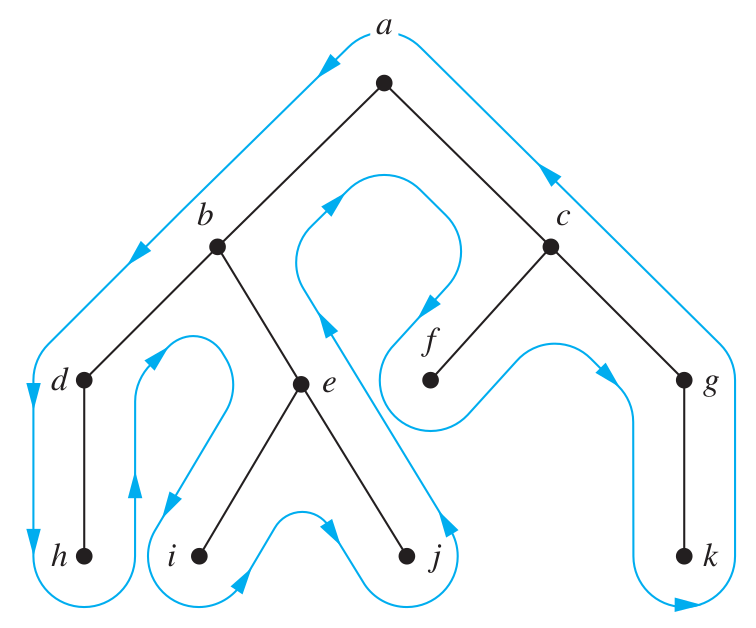
\includegraphics[width=\columnwidth]{route2}
\end{column}
\begin{column}{0.5\textwidth}
\begin{itemize}
  \item Preorder traversal gives
  $a,b,d,h$,\\$e,i,j,c,f,g,k$.
  \item Inorder traversal gives
  $h,d,b,i$,\\$e,j,a,f,c,k,g$.
  \item Postorder traversal gives
  $h,d,i,j$,\\$e,b,f,k,g,c,a$.
\end{itemize}
\end{column}
\end{columns}
\end{EXAMPLE}
\end{spacing}
\end{frame}
\begin{frame}[t,allowdisplaybreaks,allowframebreaks]{Arithmetic Operations as Trees}
\begin{spacing}{1}
\vspace*{-6pt}
Various mathematical expressions, such as compound statements in logic,
unions, intersections and differences in set theory and arithmetic operations
can be represented as ordered trees. As an example, we will discuss the
arithmetic operations $+,-,\cdot,\div,\uparrow$ (the last representing exponentiation).\\
\begin{EXAMPLE}
The expression $(x+y)^2+(x-4)/3$ can be written as $(x+y)\uparrow 2+(x-4)\div 3$. As an ordered tree, the expansion can be represented as follows:
\vspace*{-10pt}
\begin{center}
\tikzset{
my state/.style={circle,draw,fill=black,inner sep=0pt,minimum size=1.5mm}}
\begin{tikzpicture}[auto,node distance=1.4cm,on grid,every state/.style={fill=black,draw=black},line width=0.25mm]
\node[my state] (x) at (0,0) {};
\node[my state] (y) at (2,0) {};
\node[my state] (+) at (1,1) {};
\node[my state] (2) at (3,1) {};
\node[my state] (up) at (2,2) {};
\node[below=0.2cm] at (x) {$x$};
\node[below=0.2cm] at (y) {$y$};
\node[above=0.2cm] at (+) {$+$};
\node[below=0.2cm] at (2) {$2$};
\node[above=0.2cm] at (up) {$\uparrow$};
\node[my state] (xx) at (3,0) {};
\node[my state] (4) at (5,0) {};
\node[my state] (-) at (4,1) {};
\node[my state] (3) at (6,1) {};
\node[my state] (div) at (5,2) {};
\node[below=0.2cm] at (xx) {$x$};
\node[below=0.2cm] at (4) {$4$};
\node[above=0.2cm] at (-) {$-$};
\node[below=0.2cm] at (3) {$3$};
\node[above=0.2cm] at (div) {$\div$};
\node[my state] (++) at (3.5,3) {};
\node[above=0.2cm] at (++) {$+$};
\draw[-] (x) to (+) (+) to (y) (+) to (up) (up) to (2) (up) to (++) (++) to (div) (div) to (-) (-) to (xx) (-) to (4) (div) to (3);
\end{tikzpicture}
\end{center}
\end{EXAMPLE}
\end{spacing}
\end{frame}
\begin{frame}[c]{Infix Notation}
\begin{spacing}{1.1}
It is clear that an ordered binary tree of this type uniquely determines the
arithmetic expression. Note that the internal vertices of the tree
correspond to \emph{operators} while the leaves are \emph{operands}.\\[7pt]
We can list the vertices of the tree according the inorder traversal; this
gives the operators and operands of the original expression in their original
order and is known as \emph{infix notation}. However, the expression itself is not
determined by its infix notation unless parentheses are added:\\[6pt]
\begin{EXAMPLE}
The expression $(x+y)^2+(x-4)/3$ in infix notation is $x~+~y~\uparrow~2~+~x~-~4~\div~3$.
\end{EXAMPLE}
\end{spacing}
\end{frame}
\begin{frame}[t]{Prefix Notation}
\begin{spacing}{1.1}
We can also list the vertices of the tree, for example, in preorder; this is
known as \emph{prefix notation}.\\[6pt]
\begin{EXAMPLE}
The expression $(x+y)^2+(x-4)/3$ in prefix notation is $+~\uparrow~+~x~y~2~\div~-~x~4~3$.\\[5pt]
The prefix notation corresponds to listing in the order of the Universal
Address System and in this system, each binary operator will precede its
operands. thus, one can evaluate a prefix expression from right to left:
\begin{itemize}
  \item Start at the right end of the expression and read the symbols one by one. When an operator is encountered, its operands are the two symbols immediately to the right.
  \item Perform the operation on the operands; the result gives a new operand.
\end{itemize}
It can be shown (see assignments) that the prefix notation uniquely
determines the arithmetic expression without the need for parentheses.
\end{EXAMPLE}
\end{spacing}
\end{frame}
\begin{frame}[t]{Postfix Notation}
\begin{spacing}{1.1}
Finally, listing the vertices in postorder is known as \emph{postfix notation}. As
prefix notation, it does not require parentheses. A postfix expression is
evaluated from left to right:
\begin{itemize}
  \item Start at the left end of the expression and read the symbols one by one. When an operator is encountered, its operands are the two symbols immediately to the left.
  \item Perform the operation on the operands; the result gives a new operand.
\end{itemize}
\vspace*{6pt}
\begin{EXAMPLE}
The expression $(x+y)^2+(x-4)/3$ in postfix notation is $x~y~+~2~\uparrow~x~4~-~3~\div~+$.\\[6pt]
\end{EXAMPLE}
\begin{REMARK}
Postfix notation is also known as \emph{Reverse Polish Notation}.
It is used by many scientific calculators, known as \emph{RPN calculators}.
\end{REMARK}
\end{spacing}
\end{frame}
\begin{frame}[t,allowdisplaybreaks,allowframebreaks]{Spanning Trees}
\begin{spacing}{1.1}
In many applications it is of interest to find a subgraph of a graph that
includes every vertex and is also a tree.\\[6pt]
\begin{DEFINITION}
Let $G$ be a simple graph. A \emph{spanning tree} of $G$ is a
subgraph of $G$ that is a tree containing every vertex of $G$.\\[6pt]
\end{DEFINITION}
\begin{THEOREM}
A simple graph is connected if and only if it has a
spanning tree.\\[8pt]
\end{THEOREM}
\begin{PROOF}
\begin{itemize}
  \item[($\Rightarrow$)] Let $G$ be a connected graph. If $G$ has no simple circuits, then $G$ is a spanning tree of itself. If $G$ has a simple circuit, remove an edge from this circuit. The resulting subtree will remain connected. Continue removing edges until there are no more simple circuits. The result is a subgraph that is a tree and still contains all vertices of $G$. This is a spanning subtree of $G$.
\end{itemize}
\newpage
\vspace*{9pt}
\alert{Proof (continued).}\\
\begin{itemize}
  \item[($\Leftarrow$)] If a graph $G$ has a spanning tree $T$, then any two vertices of $G$ are connected by a path in $T$. Since the edges of $T$ are also edges of $G$, these vertices are connected by a path in $G$, so $G$ is a connected graph.
\end{itemize}
\end{PROOF}
\vspace*{7pt}
The method outlined in the proof of Theorem 3.4.33 (finding simple
circuits and removing edges) is not useful for finding spanning trees in
practice due to the large number of steps required to identify simple
circuits. Instead, two methods are commonly used, called \emph{depth-first
search} and \emph{breadth-first search}.
\end{spacing}
\end{frame}
\begin{frame}[t,allowdisplaybreaks,allowframebreaks]{Depth-First Search}
\begin{spacing}{1.1}
We can build a spanning tree for a connected simple graph using
\emph{depth-first search}. We will form a rooted tree, and the spanning tree will
be the underlying undirected graph of this rooted tree.
\begin{itemize}
  \item[(i)] Arbitrarily choose a vertex of the graph as the root.
  \item[(ii)] Form a path starting at this vertex by successively adding vertices and edges, where each new edge is incident with the last vertex in the path and a vertex not already in the path.
  \item[(iii)] Continue adding vertices and edges to this path as long as possible.
  \item[(iv)] If the path goes through all vertices of the graph, the tree consisting of this path is a spanning tree. If not, move back to the previous vertex in the path and attempt to add another edge as per (ii) and (iii).
\end{itemize}
\newpage
\vspace*{10pt}
Depth-first search is also called \emph{backtracking} (for obvious reasons). The
edges selected by depth-first search of a graph are called tree edges. All
other edges of the graph must connect a vertex to an ancestor or
descendant of this vertex in the tree (see assignments). These edges are
called \emph{back edges}.\\[7pt]
We say that we \emph{explore} from a vertex $v$ when we carry out the steps of
depth-first search beginning when $v$ is added to the tree and ending when
we have backtracked back to $v$ for the last time.\\[7pt]
When we add an edge connecting a vertex $v$ to a vertex $w$, we finish
exploring from $w$ before we return to $v$ to complete exploring from $v$. This
makes it easy to write a recursive algorithm for the depth-first search.
\newpage
Each edge is considered at most twice for inclusion with one of its
endpoints in $T$: once for each vertex to which it is incident. Since a
simple graph with $n$ vertices has at most $n(n-1)/2$ edges, the algorithm requires $O(n^2)$ steps.\\[6pt]
\begin{THEOREM}
The depth-first search yields a spanning tree $T$ of a connected graph $G$.\\[7pt]
\end{THEOREM}
\alert{Sketch of Proof.}\\
Let $T_0$ be the tree consisting of a single vertex of $G$. Then $T_{n+1}$ is found
from $T_n$ by adding an edge connecting a vertex in $T_n$ with a vertex not
already in $T_n$ together with this second vertex to $T_n$ and exploring from
this vertex. For each $n$, $T_n$ contains no simple circuits (prove this by
induction!) and $T_{n+1}$ is connected if $T_n$ is connected, so each $T_n$ is a tree.
Since $G$ is connected, each vertex of G will be contained in some $T_n$
(check this!), so the tree $T$ obtained after the depth-first search
terminates is a spanning tree.\hfill$\square$
\end{spacing}
\end{frame}
\begin{frame}[t]{Breadth-First Search}
\begin{spacing}{1.1}
We can also produce a spanning tree of a simple graph by the use of
\emph{breadth-first search}. Again, a rooted tree will be constructed, and the
underlying undirected graph of this rooted tree forms the spanning tree.
\begin{itemize}
  \item[(i)] Arbitrarily choose a vertex of the graph as the root.
  \item[(ii)] Add all edges incident to this vertex. The new vertices added at this stage become the vertices at level 1 in the spanning tree. Arbitrarily order them.
  \item[(iii)] For each vertex at level 1, visited in order, add each edge incident to this vertex to the tree as long as it does not produce a simple circuit. Arbitrarily order the children of each vertex at level 1. This produces the vertices at level 2 in the tree.
  \item[(iv)] Repeat (iii) until all vertices in the tree have been added.
\end{itemize}
We omit the pseudocode; like the depth-first search, this algorithm
requires $O(n^2)$ steps.
\end{spacing}
\end{frame}
\subsection{Applications of Graph Theory}
\begin{frame}[c] \begin{spacing}{2.5}
\tableofcontents[sectionstyle=hide,subsectionstyle=show/shaded/hide] \end{spacing}
\end{frame}
\begin{frame}[t]{Representing Relations as Digraphs}
\begin{spacing}{1.1}
\vspace*{-6pt}
One application of graphs is the visualization of relations, which were first introduced on Slide 118. For a relation on a set $M$, we can use a directed multigraph where we take the vertex set $V=M$ and the edge set $E=R$.
\vspace*{-6pt}
\begin{columns}[onlytextwidth]
\begin{column}{0.45\textwidth}
\begin{EXAMPLE}
Consider the relation on
\[M=\{1,2,3,4,5\}\]
given by
\[(a,b)\in R\quad\Leftrightarrow\quad
a\mid b.\]
The figure at right shows $R$ as a directed graph with vertices $V=M$ and edges $E=R$.
\end{EXAMPLE}
\end{column}
\begin{column}{0.55\textwidth}
\begin{center}
\tikzset{
my loop/.style={to path={
.. controls +(45:1.5) and +(135:1.5) .. (\tikztotarget) \tikztonodes}},
my state/.style={circle,draw,thick,inner sep=0pt,minimum size=5.5mm},
my loop2/.style={to path={
.. controls +(135:1.5) and +(225:1.5) .. (\tikztotarget) \tikztonodes}},
my loop3/.style={to path={
.. controls +(225:1.5) and +(315:1.5) .. (\tikztotarget) \tikztonodes}},
my loop4/.style={to path={
.. controls +(315:1.5) and +(405:1.5) .. (\tikztotarget) \tikztonodes}},}
\begin{tikzpicture}[->,>=stealth,line width=0.2mm,node distance=2cm,on grid,
every state/.style={draw=black,fill=white,text=black,very thick}]
\node[my state] (3) at (0,1.2) {$3$};
\node[my state] (4) at (0,-1.2) {$4$};
 \node[my state] (2) at (2.28254,1.94164) {$2$};
 \node[my state] (5) at (2.28254,-1.94164) {$5$};
 \node[my state] (1) at (3.6932,0) {$1$};
 \draw (1) to (2);
 \draw (1) to (3);
 \draw (1) to (4);
 \draw (1) to (5);
 \draw (2) to (4);
 \draw (2) to [my loop] node[]{}(2);
 \draw (3) to [my loop2] node[]{}(3);
 \draw (4) to [my loop2] node[]{}(4);
 \draw (5) to [my loop3] node[]{}(5);
 \draw (1) to [my loop4] node[]{}(1);
\end{tikzpicture}
\end{center}
\end{column}
\end{columns}
\end{spacing}
\end{frame}
\begin{frame}[t]{Partial Orderings}
\begin{spacing}{1.1}
We have previously studied equivalence relations in some depth. We now
introduce another important class of relations.\\[5pt]
\begin{DEFINITION}
Let $M$ be a set and $R$ a relation on $M$ that is reflexive,
transitive and antisymmetric (see Definition 1.4.3). Then $R$ is called a
\emph{partial ordering} on $M$ and the pair $(M,R)$ is called a \emph{partially ordered set} or \emph{poset}.\\[14pt]
\end{DEFINITION}
\begin{EXAMPLES}
\begin{enumerate}[(i)]
  \item The relation $\leq$ is a partial ordering on $\Z$. Here ``the relation $\leq$'' is supposed to mean ``the set of all pairs $(a,b)\in\Z^2$ such that $a\leq b$.'' We will use this type of shorthand throughout this section.
  \item Let $M$ be a set. The relation $\subset$ is a partial ordering on the power set $\mathcal{P}(M)$.
  \item The relation $\mid$ is a partial ordering on $\N\setminus\{0\}$.
\end{enumerate}
\end{EXAMPLES}
\end{spacing}
\end{frame}
\begin{frame}[t]{Total Orderings}
\begin{spacing}{1.1}
\vspace*{-6pt}
Given a poset $M$ we will use the general symbol $\preccurlyeq$ to indicate the ordering relation if no specific set/relation (as in the above examples) is provided. Thus, a poset is denoted $(M,\preccurlyeq)$.\\[6pt]
\begin{DEFINITION}
Let $(M,\preccurlyeq)$ be a poset.
\begin{enumerate}[(i)]
  \item Let $a,b\in M$. If $a\preccurlyeq b$ or $b\preccurlyeq a$, then $a$ and $b$ are called \emph{comparable}, otherwise they are called \emph{incomparable}.
  \item If any two elements of $M$ are comparable we say that $(M,\preccurlyeq)$ is a \emph{totally ordered} or \emph{linearly ordered} set and the relation $\preccurlyeq$ is called a \emph{total} or \emph{linear} ordering. A totally ordered set is also called a \emph{chain}.
\end{enumerate}
\end{DEFINITION}
\vspace*{6pt}
\begin{EXAMPLES}
\begin{enumerate}[(i)]
  \item The relation $\leq$ is a total ordering on $\Z$.
  \item Let $M$ be a set. The relation $\subset$ is not a total ordering on the power set $\mathcal{P}(M)$.
  \item The relation $\mid$ is not a total ordering on $\N\setminus\{0\}$.
\end{enumerate}
\end{EXAMPLES}
\end{spacing}
\end{frame}
\begin{frame}[c]{Well-Ordered Sets}
\begin{spacing}{1.1}
\begin{DEFINITION}
Let $(M,\preccurlyeq)$ be a poset. Then $(M,\preccurlyeq)$ is called a \emph{well-ordered set} if $\preccurlyeq$ is a total ordering and every non-empty subset of $M$ has a least element.\\[7pt]
\end{DEFINITION}
\begin{EXAMPLES}
\begin{enumerate}[(i)]
  \item The poset $(\Z,\leq)$ is not well-ordered, because it does not have a least element.
  \item The poset $(\N,\leq)$ is well-ordered.
  \item The poset $(\N^2,\preccurlyeq)$ with
      \[(a_1,a_2)\preccurlyeq(b_1,b_2)\qquad
      \Leftrightarrow\qquad(a_1<b_1)\vee\big((a_1=b_1)\wedge(a_2\leq b_2)\big)\]
      is well-ordered. (This is called the \emph{lexicographic ordering}.)
\end{enumerate}
\end{EXAMPLES}
\end{spacing}
\end{frame}
\begin{frame}[t]{General Lexicographic Ordering}
\begin{spacing}{1}
We can define a lexicographic ordering on the cartesian product of $n$
posets as follows:\\
\begin{DEFINITION}
Let $(A_1,\preccurlyeq_1),\,...\,,(A_n,\preccurlyeq_n)$ be a family of $n$ posets. Then the set $A_1\times\cdots\times A_n$ together with the ordering relation
\setcounter{equation}{0}
\begin{align}\label{3.5.1}
  (a_1,\,...\,,a_n)\preccurlyeq(b_1,\,...\,,b_n)\quad:\Leftrightarrow\quad &\Big(\mathop{\forall}_{1\leq i\leq n}a_1=b_i\Big)\vee\big(a_1\prec_1 b_1)\vee\nonumber \\
   &\Big(\mathop{\exists}_{j\in\{2,\,...\,,n\}}a_j\prec_j b_j\wedge\mathop{\forall}_{i<j}a_i=b_i\Big).
\end{align}
becomes a poset. The ordering relation \eqref{3.5.1} is called the \emph{lexicographic ordering} for the cartesian product $A_1\times\cdots\times A_n$.\\[7pt]
If $A_1=A_2=\cdots=A_n$ and we have the same partial order $\preccurlyeq$ on each $A_k$, we use the same symbol $\preccurlyeq$ for the partial order on the cartesian product $A_1\times\cdots\times A_n$ given by \eqref{3.5.1}.
\end{DEFINITION}
\end{spacing}
\end{frame}
\begin{frame}[c]{Lexicographic Ordering of Strings}
\begin{spacing}{1.1}
\begin{DEFINITION}
Let $\mathcal{A}$ be an alphabet and $\preccurlyeq$ an ordering relation on the alphabet. Let $a=a_1a_2\,...\,a_m$ and $b=b_1b_2\,...\,b_n$ be strings of length $n$ and $m$ from $\mathcal{A}$. Let $t=\min(m,n)$. Then we define
\begin{equation*}
  \begin{split}
     a\prec b\quad:\Leftrightarrow\quad &\big((a_1,\,...\,,a_t)=(b_1,\,...\,,b_t)\wedge
     m<n\big) \\
       &~\vee\big((a_1,\,...\,,a_t)\prec(b_1,\,...\,,b_t)\big).
  \end{split}
\end{equation*}
\vspace*{6pt}
\begin{EXAMPLE}
Let $\mathcal{A}=\{0,1\}$ with the partial ordering $\preccurlyeq$ induced by $0\prec 1$. Consider the bit strings $a=110011,\,b=11001,\,c=1100001,\,d=1110$. Then $c\prec b\prec a\prec d$.
\end{EXAMPLE}
\end{DEFINITION}
\end{spacing}
\end{frame}
\begin{frame}[t,allowdisplaybreaks,allowframebreaks]{Well-Ordered Induction}
\begin{spacing}{1.05}
Recall that the principle of induction on the natural numbers is equivalent
to the well-ordering principle. It seems plausible that a version of induction
should hold on general well-ordered sets, and this is indeed the case.\\[6pt]
If $(M,\preccurlyeq)$ is a poset and $a,b\in M$, we define
\[a\prec b\qquad:\Leftrightarrow\qquad (a\preccurlyeq b)\wedge(a\neq b).\]
 \\[9pt]
\begin{THEOREM}
Suppose that $(M,\preccurlyeq)$ is a well-ordered set. Then the predicate $P(x)$ is true for all $x\in M$ if
\begin{equation}\label{3.5.2}
\mathop{\forall}_{y\in M}~\Big(\mathop{\forall}_{x\prec y}P(x)\Big)\Rightarrow P(y)
\end{equation}
\end{THEOREM}
\newpage
\vspace*{12pt}
\begin{PROOF}
Suppose that \eqref{3.5.2} is true and that there exists some $z\in M$ so that $P(z)$ is false. Then the set $A=\{x\in M:\neg P(x)\}$ is non-empty. Since $(M,\preccurlyeq)$ is well-ordered, there exists a least element $a$ of $A$. Since $a$ is the least element of $A$, it follows that $P(x)$ is true for all $x\prec a$. But then by \eqref{3.5.2} $P(a)$ must be true. This gives a contradiction.
\end{PROOF}
\vspace*{7pt}
\begin{REMARK}
For this type of induction, we do not need a ``basis step'',
i.e., we do not need to show that $P(x)$ is true for some initial element of
$M$. For example, suppose that a is the least element of $M$. Then the statement $\mathop{\forall}\limits_{x\prec a}P(x)$ in \eqref{3.5.2} is vacuously true (there is no element $x\prec a$) so once \eqref{3.5.2} has been established, $P(a)$ is true automatically.
\end{REMARK}
\end{spacing}
\newpage
\begin{spacing}{1}
\begin{EXAMPLE}
Suppose that for $n,m\in\N$ we define
\[a_{m,n}:=\begin{cases}
             0, & \mbox{if } n=m=0, \\
             a_{m-1,n}+1, & \mbox{if } n=0~\text{and}~m>0, \\
             a_{m,n-1}+1, & \mbox{if }n>0.
           \end{cases}\]
We want to prove that
\begin{equation}\label{3.5.3}
a_{m,n}=m+\frac{n(n+1)}{2}\qquad\qquad\qquad
m,n\in\N.
\end{equation}
We can use the lexicographic ordering on $\N^2$ introduced in Example 3.5.7 to apply well-ordered induction. In particular,
\[(m,n)\prec(m_0,n_0)\quad\Leftrightarrow\quad
(m<m_0)\vee\big((m=m_0)\wedge(n<n_0)\big).\]
Take $(m_0,n_0)\in\N^2$ and suppose that \eqref{3.5.3} holds for all $(m,n)\prec(m_0,n_0)$.
\end{EXAMPLE}
\newpage
\begin{enumerate}[1.]
  \item If $(m_0,n_0)=(0,0)$ the statement follows immediately.
  \item Consider the case $n_0=0$ and $m_0>0$. Then $a_{m_0,n_0}=a_{m_0-1,n_0}+1$. Since $(m_0-1,n_0)\prec(m_0,n_0)$, we have
      \[a_{m_0,n_0}=a_{m_0-1,n_0}+1=m_0-1+\frac{n_0(n_0+1)}{2}+1=m_0+\frac{n_0(n_0+1)}{2}\]
      so \eqref{3.5.3} is true for $(m,n)=(m_0,n_0)$ in this case.
  \item Now consider the case $n_0>0$. Then $a_{m_0,n_0}=a_{m_0,n_0-1}+n_0$. Since $(m_0,n_0-1)\prec(m_0,n_0)$, we have
      \[a_{m_0,n_0}=a_{m_0,n_0-1}+n_0=m_0+\frac{n_0(n_0-1)}{2}+n_0=m_0+\frac{n_0(n_0+1)}{2}\]
      so \eqref{3.5.3} is true for $(m,n)=(m_0,n_0)$ in this case also.
\end{enumerate}
This completes the proof by induction.
\end{spacing}
\end{frame}
\begin{frame}[t,allowdisplaybreaks,allowframebreaks]{Hasse Diagrams}
\begin{spacing}{1.1}
Consider the diagraph for the poset $(\{1,2,3,4\},\leq)$:\\
\begin{columns}[onlytextwidth]
\begin{column}{0.4\textwidth}
\begin{center}
\tikzset{
my state/.style={circle,draw,thick,inner sep=0pt,minimum size=7mm},
my loop2/.style={to path={
.. controls +(135:1.5) and +(225:1.5) .. (\tikztotarget) \tikztonodes}}}
\begin{tikzpicture}[->,>=stealth,node distance=2cm,on grid,
every state/.style={draw=black,fill=white,text=black,very thick}]
\node[my state] (A) at (0,0) {$1$};
 \node[my state] (B) at (0,1.5) {$2$};
 \node[my state] (C) at (0,3) {$3$};
 \node[my state] (D) at (0,4.5) {$4$};
 \draw(A) to [my loop2] node[]{}(A);
 \draw(B) to [my loop2] node[]{}(B);
 \draw(C) to [my loop2] node[]{}(C);
 \draw(D) to [my loop2] node[]{}(D);
 \draw[->] (A) -- (B);
 \draw[->] (B) -- (C);
 \draw[->] (C) -- (D);
 \draw[->] (A) to [bend right] (C);
 \draw[->] (B) to [bend right] (D);
 \draw[->] (A) to [bend right] (D);
\end{tikzpicture}\\[7pt]
\end{center}
\end{column}
\begin{column}{0.6\textwidth}
If we know that this is the graph of a partial ordering,
we do not need to show all the edges:
\begin{itemize}
  \item Since $\leq$ is reflexive, we know that loops must be present and we can omit them,
  \item Since $\leq$ is transitive, we can omit the edges that must be present due to transitivity.
  \item If we agree that the arrows always point upwards, we can omit the arrowheads.
\end{itemize}
\end{column}
\end{columns}
\newpage
Applying these principles we end up with the following graph, called a
\emph{Hasse diagram}:
\begin{columns}[onlytextwidth]
\begin{column}{0.35\textwidth}
\begin{center}
\tikzset{
my state/.style={circle,draw,thick,inner sep=0pt,minimum size=7mm},
my loop2/.style={to path={
.. controls +(135:1.5) and +(225:1.5) .. (\tikztotarget) \tikztonodes}}}
\begin{tikzpicture}[->,>=stealth,node distance=2cm,on grid,
every state/.style={draw=black,fill=white,text=black,very thick}]
\node[my state] (A) at (0,0) {$1$};
 \node[my state] (B) at (0,1.5) {$2$};
 \node[my state] (C) at (0,3) {$3$};
 \node[my state] (D) at (0,4.5) {$4$};
 \draw[-,line width=0.25mm] (A) -- (B);
 \draw[-,line width=0.25mm] (B) -- (C);
 \draw[-,line width=0.25mm] (C) -- (D);
\end{tikzpicture}\\[7pt]
\end{center}
\end{column}
\begin{column}{0.65\textwidth}
We can perform this basic procedure with any graph
of an ordering relation. It is easy to see that the
original graph of the partial ordering relation can be
regained from the Hasse diagram, so no information
is lost by simplifying the graph in this way.\\[7pt]
The Hasse diagran can be very useful to identify basic
properties of the relation
\end{column}
\end{columns}
\newpage
\begin{EXAMPLE}
Consider the poset $(\{1,2,3,4,6,8,12\},\mid)$. Then the graph and the Hasse diagram of the relation are
\begin{center}
\begin{columns}[onlytextwidth]
\begin{column}{0.5\textwidth}
\begin{center}
\tikzset{
my state/.style={circle,draw,thick,inner sep=0pt,minimum size=7mm},
my loop2/.style={to path={
.. controls +(135:1.5) and +(225:1.5) .. (\tikztotarget) \tikztonodes}},
my loop/.style={to path={
.. controls +(315:1.5) and +(405:1.5) .. (\tikztotarget) \tikztonodes}}}
\begin{tikzpicture}[->,>=stealth,node distance=2cm,on grid,
every state/.style={draw=black,fill=white,text=black,very thick}]
\node[my state] (A) at (0,0) {$1$};
 \node[my state] (B) at (-1,1.5) {$2$};
 \node[my state] (C) at (1,1.5) {$3$};
 \node[my state] (D) at (-1,3) {$4$};
 \node[my state] (E) at (1,3) {$6$};
 \node[my state] (F) at (-1,4.5) {$8$};
 \node[my state] (G) at (1,4.5) {$12$};
 \draw (A) -- (B);
 \draw (A) -- (C);
 \draw (B) -- (D);
 \draw (D) -- (F);
 \draw (C) to (E) (E) to (G) (D) to (G) (B) to (E) (A) to (D) (A) to (F) (A) to (E) (A) to (G) (B) to (G);
 \draw (B) to [bend right] (F) (C) to [bend left] (G);
 \draw(B) to [my loop2] node[]{}(B);
 \draw(D) to [my loop2] node[]{}(D);
 \draw(F) to [my loop2] node[]{}(F);
 \draw(C) to [my loop] node[]{}(C);
 \draw(E) to [my loop] node[]{}(E);
 \draw(G) to [my loop] node[]{}(G);
\end{tikzpicture}
\end{center}
\end{column}
\begin{column}{0.5\textwidth}
\begin{center}
\tikzset{
my state/.style={circle,draw,thick,inner sep=0pt,minimum size=7mm},
my loop2/.style={to path={
.. controls +(135:1.5) and +(225:1.5) .. (\tikztotarget) \tikztonodes}},
my loop/.style={to path={
.. controls +(315:1.5) and +(405:1.5) .. (\tikztotarget) \tikztonodes}}}
\begin{tikzpicture}[-,line width=0.25mm,node distance=2cm,on grid,
every state/.style={draw=black,fill=white,text=black,very thick}]
\node[my state] (A) at (0,0) {$1$};
 \node[my state] (B) at (-1,1.5) {$2$};
 \node[my state] (C) at (1,1.5) {$3$};
 \node[my state] (D) at (-1,3) {$4$};
 \node[my state] (E) at (1,3) {$6$};
 \node[my state] (F) at (-1,4.5) {$8$};
 \node[my state] (G) at (1,4.5) {$12$};
 \draw (A) -- (B);
 \draw (A) -- (C);
 \draw (B) -- (D);
 \draw (D) -- (F);
 \draw (C) to (E) (E) to (G) (D) to (G) (B) to (E);
\end{tikzpicture}
\end{center}
\end{column}
\end{columns}
\end{center}
\end{EXAMPLE}
\end{spacing}
\end{frame}
\begin{frame}[t]{Maximal and Minimal Elements}
\begin{spacing}{1.05}
\begin{DEFINITION}
Let $(M,\preccurlyeq)$ be a poset and suppose $a\in M$. We say that\\
\begin{enumerate}[(i)]
  \item The element $a$ is \emph{maximal} if there exists no $b\in M$ such that $a\prec b$.
  \item The element $a$ is \emph{minimal} if there exists no $b\in M$ such that $b\prec a$.
  \item The element $a$ is the \emph{greatest element of $M$} if $b\preccurlyeq a$ for all $b\in M$.
  \item The element $a$ is the \emph{least element of $M$} if $a\preccurlyeq b$ for all $b\in M$.
\end{enumerate}
\begin{REMARK}
The greatest and least elements, if they exist, are unique (see exercises).
\end{REMARK}\\[6pt]
\begin{EXAMPLE}
Consider the poset $(\{1,2,3,4,6,8,12\},\mid)$ of Example 3.5.14. There,
\begin{itemize}
  \item The element 1 is minimal;
  \item The elements 8 and 12 are maximal;
  \item The element 1 is the least element;
  \item There is no greatest element.
\end{itemize}
\end{EXAMPLE}
\end{DEFINITION}
\end{spacing}
\end{frame}
\begin{frame}[t,allowdisplaybreaks,allowframebreaks]{Subsets and Bounds}
\begin{spacing}{1.1}
\vspace*{9pt}
\begin{DEFINITION}
Let $(M,\preccurlyeq)$ be a poset and suppose that $A\subset M$.
\begin{enumerate}[(i)]
  \item An element $u\in M$ such that $a\preccurlyeq u$ for all $a\in A$ is called an \emph{upper bound for $A$}.
  \item An element $I\in M$ such that $I\preccurlyeq a$ for all $a\in A$ is called a \emph{lower bound for $A$}.
  \item An upper bound $x$ for $A$ such that $x\preccurlyeq u$ for all upper bounds $u$ of $A$ is called a \emph{least upper bound for $A$}. We then write $x=\sup A$.
  \item A lower bound $x$ for $A$ such that $I\preccurlyeq x$ for all lower bounds $I$ of $A$ is called a \emph{greatest lower bound for $A$}. We then write $x=\inf A$.
\end{enumerate}
\vspace*{8pt}
\begin{REMARK}
The greatest and least upper bounds, if they exist, are
unique (see exercises).
\end{REMARK}
\end{DEFINITION}
\newpage
\begin{EXAMPLE}
Consider the poset $(\{1,2,3,4,6,8,12\},\mid)$ of Example 3.5.14 and let $A=\{1,2,3\}$. Then
\begin{itemize}
  \item The elements 6 and 12 are upper bounds for $A$;
  \item The element 1 is the (only) lower bound for $A$;
  \item $\inf A=1,\,\sup A=6$.
\end{itemize}
\end{EXAMPLE}
\begin{EXAMPLE}
Consider the poset with Hasse diagram as shown below:
\begin{columns}[onlytextwidth]
\begin{column}{0.4\textwidth}
\begin{center}
\tikzset{
my state/.style={circle,draw,thick,inner sep=0pt,minimum size=7mm},
my loop2/.style={to path={
.. controls +(135:1.5) and +(225:1.5) .. (\tikztotarget) \tikztonodes}}}
\begin{tikzpicture}[->,>=stealth,node distance=2cm,on grid,
every state/.style={draw=black,fill=white,text=black,very thick}]
\node[my state] (A) at (0,0) {$a$};
 \node[my state] (B) at (0,1.5) {$b$};
 \node[my state] (C) at (0,3) {$c$};
 \node[my state] (D) at (2,0) {$d$};
 \node[my state] (E) at (2,1.5) {$e$};
 \node[my state] (F) at (2,3) {$f$};
 \draw[-,line width=0.25mm] (A) -- (B);
 \draw[-,line width=0.25mm] (B) -- (C);
 \draw[-,line width=0.25mm] (D) -- (E);
 \draw[-,line width=0.25mm] (E) -- (F);
 \draw[-,line width=0.15mm] (B) to (D) (C) to (E) (B) to (F);
\end{tikzpicture}
\end{center}
\end{column}
\begin{column}{0.6\textwidth}
The subset $A=\{a,b,e\}$ has two upper bounds, $c$ and $f$, but no least upper bound.\\[6pt]
There is no lower bound for $A$.
\end{column}
\end{columns}
\end{EXAMPLE}
\end{spacing}
\end{frame}
\begin{frame}[t]{Lattices}
\begin{spacing}{1.05}
\begin{DEFINITION}
Let $(M,\preccurlyeq)$ be a poset and suppose that every pair of
elements of $M$ has a greatest lower and a least upper bound. Then $M$ is
called a \emph{lattice}.\\[6pt]
\end{DEFINITION}
\begin{EXAMPLE}
The left and right diagrams are lattices, the middle one is
not ($\sup\{b, c\}$ does not exist).
\begin{columns}[onlytextwidth]
\begin{column}{0.3\textwidth}
\begin{center}
\tikzset{
my state/.style={circle,draw,thick,inner sep=0pt,minimum size=7mm}}
\begin{tikzpicture}[-,line width=0.25mm,node distance=2cm,on grid,
every state/.style={draw=black,fill=white,text=black,very thick}]
\node[my state] (A) at (0,0) {$a$};
 \node[my state] (B) at (0,1) {$b$};
 \node[my state] (C) at (-1,2) {$c$};
 \node[my state] (D) at (1,2) {$d$};
 \node[my state] (E) at (0,3) {$e$};
 \node[my state] (F) at (0,4) {$f$};
 \draw[-] (A) to (B) (B) to (C) (B) to (D) (C) to (E) (E) to (D) (E) to (F);
\end{tikzpicture}
\end{center}
\end{column}
\begin{column}{0.4\textwidth}
\begin{center}
\tikzset{
my state/.style={circle,draw,thick,inner sep=0pt,minimum size=7mm}}
\begin{tikzpicture}[-,line width=0.25mm,node distance=2cm,on grid,
every state/.style={draw=black,fill=white,text=black,very thick}]
\node[my state] (A) at (0,0) {$a$};
 \node[my state] (B) at (-1,1.33333) {$b$};
 \node[my state] (C) at (1,1.33333) {$c$};
 \node[my state] (D) at (-1,2.66666) {$d$};
 \node[my state] (E) at (1,2.66666) {$e$};
 \node[my state] (F) at (0,4) {$f$};
 \draw[-] (A) to (B) (A) to (C) (B) to (D) (C) to (E) (E) to (B) (D) to (C) (D) to (F) (F) to (E);
\end{tikzpicture}
\end{center}
\end{column}
\begin{column}{0.3\textwidth}
\begin{center}
\tikzset{
my state/.style={circle,draw,thick,inner sep=0pt,minimum size=7mm},
my state2/.style={circle,draw,thick,inner sep=0pt,minimum size=6.5mm}}
\begin{tikzpicture}[-,line width=0.25mm,node distance=2cm,on grid,
every state/.style={draw=black,fill=white,text=black,very thick}]
\node[my state] (A) at (0,0) {$a$};
 \node[my state] (B) at (-1,1.33333) {$b$};
 \node[my state] (D) at (1,1.33333) {$d$};
 \node[my state] (E) at (-1,2.66666) {$e$};
 \node[my state] (G) at (1,2.66666) {$g$};
 \node[my state] (H) at (0,4) {$h$};
 \node[my state2] (C) at (0,1.33333) {$c$};
 \node[my state2] (F) at (0,2.66666) {$f$};
 \draw[-] (A) to (B) (A) to (D) (B) to (E) (D) to (G) (E) to (H) (H) to (G) (H) to (F) (F) to (C) (C) to (A);
\end{tikzpicture}
\end{center}
\end{column}
\end{columns}
\end{EXAMPLE}
\end{spacing}
\end{frame}
\begin{frame}[t,allowdisplaybreaks,allowframebreaks]{Topological Sorting}
\begin{spacing}{1.05}
Lattices are used in problems involving information flow - we will study
some examples in the exercises.\\[6pt]
We now turn to another problem: Let $(M,\preccurlyeq)$ be a poset which is not totally ordered. A total ordering $\preccurlyeq_t$ such that $a\preccurlyeq_t b$ whenever $a\preccurlyeq b$ is said to be \emph{compatible} with $\preccurlyeq$. The problem is to find a compatible total ordering for a poset $(M,\preccurlyeq)$. This is called \emph{topological sorting} of $(M,\preccurlyeq)$. In our discussion, the following result will be sueful.\\[6pt]
\begin{LEMMA}
Let $(M,\preccurlyeq)$ be a finite, non-empty poset. Then there exists a minimal element of $M$.\\[6pt]
\begin{PROOF}
Choose some $a\in M$. If $a$ is minimal, we are finished. If it is not minimal, there exists some $a_1\prec a$. We repeat this process with $a_1$. Since $M$ is finite we must obtain a minimal element after a finite number of iterations.
\end{PROOF}
\end{LEMMA}
\newpage
We now give a topological sorting algorithm as follows: Let $(M,\preccurlyeq)$ be a finite, non-empty poset.
\begin{enumerate}[1.]
  \item Find a minimal element $a_1$ of $(M,\preccurlyeq)$.
  \item Define $(M',\preccurlyeq')$, where $M'=M\setminus\{a_1\}$ and $\preccurlyeq'$ actually is the restriction of $\preccurlyeq$ from $M$ to $M'$. This is also a poset.
  \item If $M'\neq\emptyset$, repeat Step 1 with $(M,\preccurlyeq)$ replaced by $(M',\preccurlyeq')$, obtaining a least element $a_2$ of $M'$.
\end{enumerate}
The above loop continues until $M=\emptyset$. We obtain a sequence of elements $a_1,\,...\,,a_n,\,n=\text{card}\,M$, and define a total ordering $\preccurlyeq_t$ by
\[a_1\prec_t a_2\prec_t a_3\prec_t\cdots\prec_t a_n.\]
It is easy to see that $\preccurlyeq_t$ is compatible with $\preccurlyeq$: if $a\preccurlyeq b$, then $a$ will have been selected before $b$, so $a\preccurlyeq_t b$.
\newpage
\begin{EXAMPLE}
Consider the poset $(\{1,2,3,4,6,8,12\},\mid)$ of Example 3.5.14. Then a total ordering can be found by successively choosing the least (bottom) elements from the Hasse diagram:
\begin{columns}[onlytextwidth]
\begin{column}{0.45\textwidth}
\begin{center}
\tikzset{
my state/.style={circle,draw,thick,inner sep=0pt,minimum size=7mm},
my loop2/.style={to path={
.. controls +(135:1.5) and +(225:1.5) .. (\tikztotarget) \tikztonodes}},
my loop/.style={to path={
.. controls +(315:1.5) and +(405:1.5) .. (\tikztotarget) \tikztonodes}}}
\begin{tikzpicture}[-,line width=0.25mm,node distance=2cm,on grid,
every state/.style={draw=black,fill=white,text=black,very thick}]
\node[my state] (A) at (0,0) {$1$};
 \node[my state] (B) at (-1,1.5) {$2$};
 \node[my state] (C) at (1,1.5) {$3$};
 \node[my state] (D) at (-1,3) {$4$};
 \node[my state] (E) at (1,3) {$6$};
 \node[my state] (F) at (-1,4.5) {$8$};
 \node[my state] (G) at (1,4.5) {$12$};
 \draw (A) -- (B);
 \draw (A) -- (C);
 \draw (B) -- (D);
 \draw (D) -- (F);
 \draw (C) to (E) (E) to (G) (D) to (G) (B) to (E);
\end{tikzpicture}
\end{center}
\end{column}
\begin{column}{0.55\textwidth}
One possible total ordering is given by
\[1\prec_t 2\prec_t 3\prec_t 4\prec_t 6\prec_t 8\prec_t 12\]
Another possibility is
\[1\prec_t 3\prec_t 2\prec_t 6\prec_t 4\prec_t 12\prec_t 8\]
\end{column}
\end{columns}
\end{EXAMPLE}
\end{spacing}
\end{frame}
\begin{frame}[t,allowdisplaybreaks,allowframebreaks]{A Simple Proof of Fermat's Little Theorem}
\begin{spacing}{1.05}
\vspace*{11pt}
We now compile some more applications of graph theory. Recall the
Fermat's Little Theorem 1.9.2 from the first part of the course:\\[6pt]
\stepcounter{zhuo}
\alert{3.5.26. Fermat's Little Theorem.} Let $p\in\N$ and $a\in\N$. If $p$ is prime, then
\begin{equation}\label{3.5.4}
p\mid(a^p-a).
\end{equation}
We now give a quick and elegant proof using graph theory.
\end{spacing}
\newpage
\begin{spacing}{0.9}
\begin{PROOF}
Let $G=(V,E)$ be the graph with vertex set
\[V=\Big\{(a_1,\,...\,,a_p)\in\N^p\!:\mathop{\forall}_{k=1,\,...\,,p}
1\leq a_k\leq a~\text{and}~\mathop{\exists}_{1\leq i,j\leq p}a_i\neq a_j\Big\}\]
Then
\[\text{card}\,V=a^p-a.\]
For any $u=(u_1,\,...\,,u_p)\in V$ we also have $v=(u_p,u_1,\,...\,,u_{p-1})\in V$ and we let $\{u,v\}\in E$. In particular, $E$ is precisely the set of all such two-element sets of $p$-tuples.\\
Then each vertex of $G$ has degree two and (since $p$ is prime) the
connected components of $G$ are cycles of length $p$. Since the number of
connected components is an integer, we must have
\[p\mid(a^p-a).\]
\end{PROOF}
\end{spacing}
\end{frame}
\begin{frame}[t,allowdisplaybreaks,allowframebreaks]{A Proof of the Cantor-Schr\"{o}der-Bernstein Theorem}
\begin{spacing}{1}
Recall that we defined the size (cardinality) of sets by comparing them
using maps (see Definition 2.4.1):\\[5pt]
\begin{DEFINITION}
Let $A,B$ be arbitrary sets. Then
\begin{align*}
  \text{card}\,A&\leq\text{card}\,B & &:\Leftrightarrow & \exists~\varphi\!:\,A&\to B~\text{injective},  \\
  \text{card}\,A&=\text{card}\,B & &:\Leftrightarrow & \exists~\varphi\!:\,A&\to B~\text{bijective}.
\end{align*}
We would then expect that
\[\text{card}\,A\leq\text{card}\,B\qquad\wedge\qquad
\text{card}\,B\leq\text{card}\,A\qquad\Rightarrow\qquad
\text{card}\,A=\text{card}\,B.\]
or, in words:\\[5pt]
\stepcounter{zhuo}
\alert{3.5.28. Cantor-Schr\"{o}der-Bernstein Theorem.} Let $A, B$ be arbitrary sets. If
there exist injective maps from $A$ to $B$ and from $B$ to $A$, then there exists
a bijective map between $A$ and $B$.
\end{DEFINITION}
\newpage
\vspace*{9pt}
\begin{PROOF}
Suppose that there exist injective maps $\varphi\!:\,A\to B,\psi\!:\,B\to A$. We define
a 2-colored (bipartite) graph $G = (A, B, E)$ as follows: one set of vertices
is colored red and labeled with the elements of $A$, the other set is colored
blue and labeled with the elements of $B$.\\[7pt]
We denote these vertex sets by $A$ and $B$ also, keeping in mind that due to
their colorings they are now disjoint. In fact, we can now assume without
loss of generality that the original sets $A$ and $B$ are disjoint. (If they are
not, we just add the color of each element to distinguish identical
elements.)\\[6pt]
Of course, $G$ may have an infinite (even uncountable) number of vertices.
\newpage
\vspace*{10pt}
\alert{Proof (continued).}\\
Let us define a relation on $A\cup B$ by setting
\[a\sim b\qquad\qquad\qquad:\Leftrightarrow\qquad\qquad\qquad
b=\varphi(a)\qquad\vee\qquad a=\psi(b).\]
The edge set of $G$ is now defined by letting $G$ be the directed graph
representing this relation.\\[7pt]
Every vertex in $G$ is the initial vertex of an edge, since $\varphi$ is defined on all of $A$ and $\psi$ is defined on all of $B$. Furthermore, every vertex is the terminal vertex of at most one edge, since $\varphi$ and $\psi$ are injective. Hence, the degree of each vertex is either 1 or 2.
\newpage
\alert{Proof (continued).}\\
We now examine the connected components of $G$. These can take the
following forms:
\begin{itemize}
  \item A finite, simple circuit of even length,
  \item An infinite path with initial vertex $v_0,\,(v_0,v_1,v_2,\,...)$,
  \item An infinite path with no initial vertex, $(...\,,v_{-2},v_{-1},v_0,v_1,v_2,\,...)$.
\end{itemize}
Since every vertex is the initial vertex of a directed edge, there can be no
finite paths that are not circuits. All circuits must be of even length by
Theorem 3.3.16, so the above list is complete.\\[7pt]
In each connected component we now remove every second directed edge.
The remaining edges then give a one-to-one pairing between vertices of $A$
and of $B$ in each connected component. Hence, the cardinalities of the
vertex sets associated to $A$ and $B$ in each component is the same and so
the cardinalities of $A$ and $B$ are equal overall.
\end{PROOF}
\end{spacing}
\end{frame}
\subsection{Generating Functions}
\begin{frame}[c] \begin{spacing}{2.5}
\tableofcontents[sectionstyle=hide,subsectionstyle=show/shaded/hide] \end{spacing}
\end{frame}
\begin{frame}[t,allowdisplaybreaks,allowframebreaks]{Counting Full Binary Trees}
\begin{spacing}{1.05}
Let us ask a seemingly simple question: how many different full binary
trees with $n\in\N\setminus\{0\}$ internal vertices are there?\\[6pt]
This question is related to the number of ways of sorting a list on elements,
since a binary sorting algorithm can be represented as a binary tree with
leaves corresponding to final arrangements of the list after sorting.
In order to get a grasp on the question, it is useful to introduce an
alternative, recursive definition of full binary trees:\\[5pt]
\begin{DEFINITION}
\begin{enumerate}[(i)]
  \item The tree consisting of a single vertex $r$ is a \emph{full binary tree} with root $r$.
  \item If $T_1$ and $T_2$ are full binary trees, then the rooted tree formed by adding a new vertex $r$ and edges joining r to the roots of $T_1$ and $T_2$ is a full binary tree with root $r$.
\end{enumerate}
The equivalence with Definition 3.4.7 can be shown using structural
induction and strong induction.
\end{DEFINITION}
\newpage
We can now argue as follows: A binary tree with $n$ internal vertices has a
root and two subtrees with a total of $n -1$ vertices. If $C_n$ denotes the
number of full binary trees with $n$ internal vertices, we then have
\setcounter{equation}{0}
\begin{equation}\label{3.6.1}
C_n=\sum_{i+j=n-1}C_iC_j=\sum_{k=0}^{n-1}C_kC_{n-1-k},\qquad\qquad
n\geq2.
\end{equation}
where the sum on the right is found by counting all possible forms of the
two subtrees of the root. We also have
\[C_0=C_1=1\]
so \eqref{3.6.1} defines a (non-linear) recurrence relation for $C_n$. In order to
solve the relation, we need to develop a new and useful tool: generating
functions.
\end{spacing}
\end{frame}
\begin{frame}[t,allowdisplaybreaks,allowframebreaks]{Generating Functions}
\begin{spacing}{1.05}
\vspace*{9pt}
In this section, we introduce a very powerful tool from calculus that can be
used to solve recurrence relations or obtain combinatorial identities: the
generating function of a sequence.\\[6pt]
\begin{DEFINITION}
Let $(a_n)$ be a sequence of real numbers. If the formal power series
\[G(x)=\sum_{n=0}^{\infty}a_nx^n=a_0+a_1x+a_2x^2+\,...\]
has a radius of convergence $\varrho>0$ we say that $G$ is a \emph{generating function} for $(a_n)$.\\[6pt]
If $(a_0,\,...\,,a_k)$ is a finite tuple, we define the generating function in the same way, regarding the tuple as a sequence $(a_n)$ with $a_n=0$ for $n>k$.
\end{DEFINITION}
\newpage
\begin{EXAMPLES}
\begin{itemize}
  \item[(i)] The geometric series formula yields
      \[\sum_{n=0}^{\infty}x^n=\frac{1}{1-x}=:G(x)\qquad\qquad\qquad
      \text{for}\,|x|<1\]
      so $G$ is the generating function for the sequence $(a_n)$ with $a_n=1$ for all $n\in\N$.
  \item[(ii)] Consider the $(1,\,a,\,a^2,\,a^3,\,...)$ for some $a\in\R$. This sequence has generating function
      \[G(x)=\frac{1}{1-ax}=\sum_{n=0}^{\infty}a^nx^n\]
      where the series has radius of convergence $\varrho=1/a$.
\newpage
\vspace*{11pt}
  \item[(iii)] By the binomial theorem,
      \[(1+x)^n=\sum_{k=0}^{n}\binom{n}{k}x^k\]
      so the function $G(x)=(1+x)^n$ is the generating function for the $n+1$-tuple
      \[\binom{n}{0},\binom{n}{1},\,...\,,\binom{n}{n}.\]
\end{itemize}
\end{EXAMPLES}
\end{spacing}
\end{frame}
\begin{frame}[t,allowdisplaybreaks,allowframebreaks]{The Cauchy Product}
\begin{spacing}{1}
Generating functions are power series with non-vanishing radii of
convergence. In order to work with them effectively, we need to recall
some background from calculus. In particular, we have the following result
regarding the product of two power series:\\
\begin{THEOREM}
Let $\sum a_k$ and $\sum b_k$ be series that both converge absolutely. Then the \emph{Cauchy product} $\sum c_k$,
\[c_k:=\sum_{i+j=k}a_ib_j\]
converges absolutely and $\sum c_k=\Big(\sum a_k\Big)\Big(\sum b_k\Big)$. The sequence
\[(a_k)\ast(b_k):=(c_k),\qquad\qquad\qquad c_k:=\sum_{i+j=k}a_ib_j,\]
is called the \emph{convolution} of the sequences $(a_k)$ and $(b_k)$.
\end{THEOREM}
\newpage
\begin{EXAMPLE}
The Cauchy product is often used in calculus to establish
the functional equation for the exponential function. The exponential
function can be defined to be
\[\exp(x)=\sum_{n=0}^{\infty}\frac{x^n}{n!}.\]
Then
\begin{equation*}
  \begin{split}
     (\exp x)(\exp y) &=\Big(\sum_{n=0}^{\infty}\frac{x^n}{n!}\Big)\Big(\sum_{m=0}^{\infty}\frac{y^m}{m!}\Big)
     =\sum_{n=0}^{\infty}\bigg(\Big(\frac{x^k}{k!}\Big)\ast\Big(\frac{y^k}{k!}\Big)\bigg)_n \\
       &=\sum_{n=0}^{\infty}\sum_{l+m=n}\frac{1}{l!m!}x^ly^m=\sum_{n=0}^{\infty}\frac{1}{n!}
       \sum_{l+m=n}\frac{n!}{l!m!}x^ly^m \\
       &=\sum_{n=0}^{\infty}\frac{1}{n!}(x+y)^n \\
       &=\exp(x+y)
  \end{split}
\end{equation*}
\end{EXAMPLE}
\!\!This yields the functional equation
\[(\exp x)(\exp y)=\exp(x+y).\]
We also remark that $\exp x=e^x$ is the generating function for the sequence $(a_n)$ with $a_n=1/n!$.\\[6pt]
\begin{COROLLARY}
Let $\sum a_kx^k$ and $\sum b_kx^k$ be power series that both converge absolutely for $|x|<\varrho$. Then
\[\Big(\sum_{l=0}^{\infty}a_lx^l\Big)\Big(\sum_{m=0}^{\infty}b_mx^m\Big)
=\sum_{n=0}^{\infty}c_nx^n\]
with
\[c_n=\sum_{i+j=n}a_ib_j\]
\end{COROLLARY}
\newpage
\begin{EXAMPLE}
For any $n\in\Z_+$ and $k=0,\,...\,,n$,
\[\binom{n}{0}\binom{n}{k}+\binom{n}{1}\binom{n}{k-1}+\cdots+\binom{n}{k}\binom{n}{0}
=\binom{2n}{k}.\]
We can write this identity as
\begin{equation}\label{3.6.2}
\sum_{i=0}^{k}\binom{n}{i}\binom{n}{k-i}=\sum_{i+j=k}\binom{n}{i}
\binom{n}{j}=\binom{2n}{k}
\end{equation}
To prove \eqref{3.6.2}, we consider the generating function of the finite sequence $\binom{2n}{k},\,k=0,\,...\,,2n$, given by
\begin{equation}\label{3.6.3}
G(x)=(1+x)^{2n}=\sum_{k=0}^{2n}\binom{2n}{k}x^k.
\end{equation}
\end{EXAMPLE}
\end{spacing}
\newpage
\begin{spacing}{0.4}
For $k=0,\,...\,,n$ the right-hand-side of \eqref{3.6.2} is given by the coefficient of $x^k$ in $G(x)$. Now
\begin{equation*}
  \begin{split}
     (1+x)^{2n} &=\big((1+x)^n\big)^2 \\
       &=\Big(\sum_{l=0}^{n}\binom{n}{l}x^l\Big)\Big(\sum_{m=0}^{n}\binom{n}{m}x^m\Big) \\
       &=\sum_{k=0}^{2n}\Big(\sum_{i+j=k}\binom{n}{i}\binom{n}{j}\Big)x^k.
  \end{split}
\end{equation*}
Comparing with \eqref{3.6.3} gives \eqref{3.6.2}. The formula \eqref{3.6.2} was known to the Chinese mathematician Zhu Shijie (朱世杰) who lived around AD 1300. Setting $k=n$ we obtain the special case
\[\sum_{k=0}^{n}\binom{n}{k}^2=\binom{2n}{n},\]
which is known as \emph{Vandermonde's convolution formula}.
\end{spacing}
\end{frame}
\begin{frame}[t,allowdisplaybreaks,allowframebreaks]{The Binomial Series}
\begin{spacing}{1.05}
We will need some more background from basic calculus to employ
generating functions to their full potential. Recall that the generalized
binomial coefficients are defined by
\[\binom{\alpha}{0}:=1,\qquad\quad\binom{\alpha}{j}:=
\frac{\alpha(\alpha-1)\,...\,(\alpha-j+1)}{j!},\qquad\quad
j\in\N,\,\alpha\in\R.\]
The following theorem should be known from calculus:\\[6pt]
\begin{THEOREM}
Let $-1<x<1$ and $\alpha\in\R$. Then
\[(1+x)^\alpha=\sum_{n=0}^{\infty}\binom{\alpha}{n}x^n\]
where the series on the right converges absolutely.
\end{THEOREM}
\end{spacing}
\newpage
\begin{spacing}{0.75}
\begin{EXAMPLE}
For $\alpha=1/2$, we have the binomial series
\[\sqrt{1+x}=\sum_{n=0}^{\infty}\binom{1/2}{n}x^n.\]
The first term, $n=0$, evaluates to
\[\binom{1/2}{0}x^0=1.\]
For $n\geq1$ we have
\begin{equation*}
  \begin{split}
     \binom{1/2}{n} &=\frac{1/2(1/2-1)(1/2-2)\,...\,(1/2-(n-1))}{n!} \\
       &=(-1)^{n-1}\frac{1/2(1-1/2)(2-1/2)\,...\,(n-1-1/2)}{n!} \\
       &=\frac{(-1)^{n-1}}{2^n}\frac{1(2-1)(4-1)\,...\,(2(n-1)-1)}{n!}
  \end{split}
\end{equation*}
\end{EXAMPLE}
\!\!Continuing,
\begin{equation*}
  \begin{split}
     \binom{1/2}{n} &=\frac{(-1)^{n-1}}{2^n}\frac{1(2-1)(4-1)\,...\,(2(n-1)-1)}{n!} \\
       &=\frac{(-1)^{n-1}}{2^n}\frac{1\cdot1\cdot3\cdot5\cdots(2n-3)}{n!} \\
       &=\frac{(-1)^{n-1}}{2^n}\frac{1}{2^{n-1}(n-1)!}\frac{1\cdot2\cdot3\cdot4\cdot5\cdots(2n-2)}{n!} \\
       &=-2\frac{(-1)^n}{4^n}\frac{1}{n}\frac{(2n-2)!}{n(n-1)!(n-1)!}=-2\frac{(-1)^n}{4^n}\frac{1}{n}
       \binom{2n-2}{n-1}.
  \end{split}
\end{equation*}
It follows that
\begin{equation}\label{3.6.4}
\sqrt{1+x}=1-2\sum_{n=1}^{\infty}\frac{(-1)^n}{4^n}
\binom{2n-2}{n-1}\frac{x^n}{n}
\end{equation}
for $|x|<1$.
\end{spacing}
\end{frame}
\begin{frame}[t,allowdisplaybreaks,allowframebreaks]{Counting Full Binary Trees}
\begin{spacing}{0.9}
We will now find a closed formula for the numbers $C_n$. Recall that they
satisfy the recurrence relation \eqref{3.6.1},
\[C_{n+1}=\sum_{k=0}^{n}C_kC_{n-k}=\sum_{j+k=n}C_kC_j,\qquad\qquad\qquad
n\in\N.\]
with $C_0=1$. We define the generating function of the sequence $(C_n)$ to be the formal power series
\[c(x):=\sum_{n=0}^{\infty}C_nx^n.\]
Then
\begin{equation*}
  \begin{split}
     c(x)^2 &=\Big(\sum_{j=0}^{\infty}C_jx^j\Big)\Big(\sum_{k=0}^{\infty}C_kx^k\Big)
     =\sum_{n=0}^{\infty}\Big(\sum_{j+k=n}C_kC_j\Big)x^n \\
       &=\sum_{n=0}^{\infty}C_{n+1}x^n=\frac{1}{x}(c(x)-1)
  \end{split}
\end{equation*}
\newpage
It follows that
\[c(x)=1+xc(x)^2.\]
This implies that
\[c(x)=\frac{1-\sqrt{1-4x}}{2x}=\frac{2}{1+\sqrt{1-4x}}\]
From the last quotient we see that $c(x)$ actually has a power series expansion at $x=0$. Expanding the first quotient using \eqref{3.6.4},
\begin{equation*}
  \begin{split}
     c(x) &=\frac{1}{2x}(1-\sqrt{1-4x})=\frac{1}{2x}\cdot2\sum_{n=1}^{\infty}\frac{(-1)^n}{4^n}
     \binom{2n-2}{n-1}\frac{(-4x)^n}{n} \\
       &=\sum_{n=1}^{\infty}\binom{2n-2}{n-1}\frac{x^{n-1}}{n} \\
       &=\sum_{n=0}^{\infty}\binom{2n}{n}\frac{x^n}{n+1}=\sum_{n=0}^{\infty}C_nx^n.
  \end{split}
\end{equation*}
\end{spacing}
\end{frame}
\begin{frame}[c]{The Catalan Numbers}
\begin{spacing}{1.1}
This shows that the number of full binary trees with $n$ internal vertices is
given by
\[C_n=\frac{1}{n+1}\binom{2n}{n},\qquad\qquad\qquad\quad
n\in\N.\]
These numbers are called the \emph{Catalan numbers}. They appear in many contexts, e.g., as
\begin{itemize}
  \item The number of ways to parenthesize the product of $n + 1$ numbers (cf. Example 8, page 456 of \emph{Rosen}),
  \item The number of non-crossing handshakes of $2n$ people seated across a circular table,
  \item The number of triangulations of a polygon with $n + 2$ sides,
  \item The number of rooted trees with $n$ edges.
\end{itemize}
\end{spacing}
\end{frame}
%%%%%%%%%%%%%%%%%%%%%%%%%%%%%%%%%%%%
%%%%%  This is the end of Ve203.
%%%%%  I spent 2000 lines more than
%%%%%  Vv285, for I applied pgf into
%%%%%  into my text. Altogether 12128
%%%%%  lines. Finished at 2:44:05 2016/3/15  By Wang Yuzhuo.
\end{document} 